\documentclass[twoside]{book}

% Packages required by doxygen
\usepackage{fixltx2e}
\usepackage{calc}
\usepackage{doxygen}
\usepackage[export]{adjustbox} % also loads graphicx
\usepackage{graphicx}
\usepackage[utf8]{inputenc}
\usepackage{makeidx}
\usepackage{multicol}
\usepackage{multirow}
\PassOptionsToPackage{warn}{textcomp}
\usepackage{textcomp}
\usepackage[nointegrals]{wasysym}
\usepackage[table]{xcolor}

% Font selection
\usepackage[T1]{fontenc}
\usepackage[scaled=.90]{helvet}
\usepackage{courier}
\usepackage{amssymb}
\usepackage{sectsty}
\renewcommand{\familydefault}{\sfdefault}
\allsectionsfont{%
  \fontseries{bc}\selectfont%
  \color{darkgray}%
}
\renewcommand{\DoxyLabelFont}{%
  \fontseries{bc}\selectfont%
  \color{darkgray}%
}
\newcommand{\+}{\discretionary{\mbox{\scriptsize$\hookleftarrow$}}{}{}}

% Page & text layout
\usepackage{geometry}
\geometry{%
  a4paper,%
  top=2.5cm,%
  bottom=2.5cm,%
  left=2.5cm,%
  right=2.5cm%
}
\tolerance=750
\hfuzz=15pt
\hbadness=750
\setlength{\emergencystretch}{15pt}
\setlength{\parindent}{0cm}
\setlength{\parskip}{3ex plus 2ex minus 2ex}
\makeatletter
\renewcommand{\paragraph}{%
  \@startsection{paragraph}{4}{0ex}{-1.0ex}{1.0ex}{%
    \normalfont\normalsize\bfseries\SS@parafont%
  }%
}
\renewcommand{\subparagraph}{%
  \@startsection{subparagraph}{5}{0ex}{-1.0ex}{1.0ex}{%
    \normalfont\normalsize\bfseries\SS@subparafont%
  }%
}
\makeatother

% Headers & footers
\usepackage{fancyhdr}
\pagestyle{fancyplain}
\fancyhead[LE]{\fancyplain{}{\bfseries\thepage}}
\fancyhead[CE]{\fancyplain{}{}}
\fancyhead[RE]{\fancyplain{}{\bfseries\leftmark}}
\fancyhead[LO]{\fancyplain{}{\bfseries\rightmark}}
\fancyhead[CO]{\fancyplain{}{}}
\fancyhead[RO]{\fancyplain{}{\bfseries\thepage}}
\fancyfoot[LE]{\fancyplain{}{}}
\fancyfoot[CE]{\fancyplain{}{}}
\fancyfoot[RE]{\fancyplain{}{\bfseries\scriptsize Generated by Doxygen }}
\fancyfoot[LO]{\fancyplain{}{\bfseries\scriptsize Generated by Doxygen }}
\fancyfoot[CO]{\fancyplain{}{}}
\fancyfoot[RO]{\fancyplain{}{}}
\renewcommand{\footrulewidth}{0.4pt}
\renewcommand{\chaptermark}[1]{%
  \markboth{#1}{}%
}
\renewcommand{\sectionmark}[1]{%
  \markright{\thesection\ #1}%
}

% Indices & bibliography
\usepackage{natbib}
\usepackage[titles]{tocloft}
\setcounter{tocdepth}{3}
\setcounter{secnumdepth}{5}
\makeindex

% Hyperlinks (required, but should be loaded last)
\usepackage{ifpdf}
\ifpdf
  \usepackage[pdftex,pagebackref=true]{hyperref}
\else
  \usepackage[ps2pdf,pagebackref=true]{hyperref}
\fi
\hypersetup{%
  colorlinks=true,%
  linkcolor=blue,%
  citecolor=blue,%
  unicode%
}

% Custom commands
\newcommand{\clearemptydoublepage}{%
  \newpage{\pagestyle{empty}\cleardoublepage}%
}

\usepackage{caption}
\captionsetup{labelsep=space,justification=centering,font={bf},singlelinecheck=off,skip=4pt,position=top}

%===== C O N T E N T S =====

\begin{document}

% Titlepage & ToC
\hypersetup{pageanchor=false,
             bookmarksnumbered=true,
             pdfencoding=unicode
            }
\pagenumbering{alph}
\begin{titlepage}
\vspace*{7cm}
\begin{center}%
{\Large A\+WS IoT Device Client }\\
\vspace*{1cm}
{\large Generated by Doxygen 1.8.13}\\
\end{center}
\end{titlepage}
\clearemptydoublepage
\pagenumbering{roman}
\tableofcontents
\clearemptydoublepage
\pagenumbering{arabic}
\hypersetup{pageanchor=true}

%--- Begin generated contents ---
\chapter{Hierarchical Index}
\doxysection{Class Hierarchy}
This inheritance list is sorted roughly, but not completely, alphabetically\+:\begin{DoxyCompactList}
\item \contentsline{section}{Aws\+::Iot\+::Device\+Client\+::Client\+Base\+Notifier}{\pageref{class_aws_1_1_iot_1_1_device_client_1_1_client_base_notifier}}{}
\begin{DoxyCompactList}
\item \contentsline{section}{Aws\+::Iot\+::Device\+Client\+::Default\+Client\+Base\+Notifier}{\pageref{class_aws_1_1_iot_1_1_device_client_1_1_default_client_base_notifier}}{}
\end{DoxyCompactList}
\item \contentsline{section}{Aws\+::Iot\+::Device\+Client\+::Config}{\pageref{class_aws_1_1_iot_1_1_device_client_1_1_config}}{}
\item \contentsline{section}{Aws\+::Iot\+::Device\+Client\+::Util\+::Retry\+::Exponential\+Retry\+Config}{\pageref{struct_aws_1_1_iot_1_1_device_client_1_1_util_1_1_retry_1_1_exponential_retry_config}}{}
\item \contentsline{section}{Aws\+::Iot\+::Device\+Client\+::Feature}{\pageref{class_aws_1_1_iot_1_1_device_client_1_1_feature}}{}
\begin{DoxyCompactList}
\item \contentsline{section}{Aws\+::Iot\+::Device\+Client\+::Device\+Defender\+::Device\+Defender\+Feature}{\pageref{class_aws_1_1_iot_1_1_device_client_1_1_device_defender_1_1_device_defender_feature}}{}
\item \contentsline{section}{Aws\+::Iot\+::Device\+Client\+::Jobs\+::Jobs\+Feature}{\pageref{class_aws_1_1_iot_1_1_device_client_1_1_jobs_1_1_jobs_feature}}{}
\item \contentsline{section}{Aws\+::Iot\+::Device\+Client\+::Secure\+Tunneling\+::Secure\+Tunneling\+Feature}{\pageref{class_aws_1_1_iot_1_1_device_client_1_1_secure_tunneling_1_1_secure_tunneling_feature}}{}
\end{DoxyCompactList}
\item \contentsline{section}{Aws\+::Iot\+::Device\+Client\+::Util\+::File\+Utils}{\pageref{class_aws_1_1_iot_1_1_device_client_1_1_util_1_1_file_utils}}{}
\item \contentsline{section}{Aws\+::Iot\+::Device\+Client\+::Fleet\+Provisioning\+NS\+::Fleet\+Provisioning}{\pageref{class_aws_1_1_iot_1_1_device_client_1_1_fleet_provisioning_n_s_1_1_fleet_provisioning}}{}
\item \contentsline{section}{Aws\+::Iot\+::Device\+Client\+::Jobs\+::Job\+Engine}{\pageref{class_aws_1_1_iot_1_1_device_client_1_1_jobs_1_1_job_engine}}{}
\item \contentsline{section}{Aws\+::Iot\+::Device\+Client\+::Jobs\+::Jobs\+Feature\+::Job\+Execution\+Status\+Info}{\pageref{struct_aws_1_1_iot_1_1_device_client_1_1_jobs_1_1_jobs_feature_1_1_job_execution_status_info}}{}
\item \contentsline{section}{Aws\+::Iot\+::Device\+Client\+::Jobs\+::Limited\+Stream\+Buffer}{\pageref{class_aws_1_1_iot_1_1_device_client_1_1_jobs_1_1_limited_stream_buffer}}{}
\item \contentsline{section}{Aws\+::Iot\+::Device\+Client\+::Loadable\+From\+Json\+And\+Cli\+And\+Environment}{\pageref{class_aws_1_1_iot_1_1_device_client_1_1_loadable_from_json_and_cli_and_environment}}{}
\begin{DoxyCompactList}
\item \contentsline{section}{Aws\+::Iot\+::Device\+Client\+::Plain\+Config}{\pageref{struct_aws_1_1_iot_1_1_device_client_1_1_plain_config}}{}
\item \contentsline{section}{Aws\+::Iot\+::Device\+Client\+::Plain\+Config\+::Device\+Defender}{\pageref{struct_aws_1_1_iot_1_1_device_client_1_1_plain_config_1_1_device_defender}}{}
\item \contentsline{section}{Aws\+::Iot\+::Device\+Client\+::Plain\+Config\+::Fleet\+Provisioning}{\pageref{struct_aws_1_1_iot_1_1_device_client_1_1_plain_config_1_1_fleet_provisioning}}{}
\item \contentsline{section}{Aws\+::Iot\+::Device\+Client\+::Plain\+Config\+::Fleet\+Provisioning\+Runtime\+Config}{\pageref{struct_aws_1_1_iot_1_1_device_client_1_1_plain_config_1_1_fleet_provisioning_runtime_config}}{}
\item \contentsline{section}{Aws\+::Iot\+::Device\+Client\+::Plain\+Config\+::Jobs}{\pageref{struct_aws_1_1_iot_1_1_device_client_1_1_plain_config_1_1_jobs}}{}
\item \contentsline{section}{Aws\+::Iot\+::Device\+Client\+::Plain\+Config\+::Log\+Config}{\pageref{struct_aws_1_1_iot_1_1_device_client_1_1_plain_config_1_1_log_config}}{}
\item \contentsline{section}{Aws\+::Iot\+::Device\+Client\+::Plain\+Config\+::Tunneling}{\pageref{struct_aws_1_1_iot_1_1_device_client_1_1_plain_config_1_1_tunneling}}{}
\end{DoxyCompactList}
\item \contentsline{section}{Aws\+::Iot\+::Device\+Client\+::Logging\+::Logger}{\pageref{class_aws_1_1_iot_1_1_device_client_1_1_logging_1_1_logger}}{}
\begin{DoxyCompactList}
\item \contentsline{section}{Aws\+::Iot\+::Device\+Client\+::Logging\+::File\+Logger}{\pageref{class_aws_1_1_iot_1_1_device_client_1_1_logging_1_1_file_logger}}{}
\item \contentsline{section}{Aws\+::Iot\+::Device\+Client\+::Logging\+::Std\+Out\+Logger}{\pageref{class_aws_1_1_iot_1_1_device_client_1_1_logging_1_1_std_out_logger}}{}
\end{DoxyCompactList}
\item \contentsline{section}{Aws\+::Iot\+::Device\+Client\+::Logging\+::Logger\+Factory}{\pageref{class_aws_1_1_iot_1_1_device_client_1_1_logging_1_1_logger_factory}}{}
\item \contentsline{section}{Aws\+::Iot\+::Device\+Client\+::Logging\+::Log\+Message}{\pageref{class_aws_1_1_iot_1_1_device_client_1_1_logging_1_1_log_message}}{}
\item \contentsline{section}{Aws\+::Iot\+::Device\+Client\+::Logging\+::Log\+Queue}{\pageref{class_aws_1_1_iot_1_1_device_client_1_1_logging_1_1_log_queue}}{}
\item \contentsline{section}{Aws\+::Iot\+::Device\+Client\+::Permissions}{\pageref{struct_aws_1_1_iot_1_1_device_client_1_1_permissions}}{}
\item promise\begin{DoxyCompactList}
\item \contentsline{section}{Aws\+::Iot\+::Device\+Client\+::Jobs\+::Ephemeral\+Promise$<$ T $>$}{\pageref{class_aws_1_1_iot_1_1_device_client_1_1_jobs_1_1_ephemeral_promise}}{}
\end{DoxyCompactList}
\item \contentsline{section}{Aws\+::Iot\+::Device\+Client\+::Util\+::Retry}{\pageref{class_aws_1_1_iot_1_1_device_client_1_1_util_1_1_retry}}{}
\item \contentsline{section}{Aws\+::Iot\+::Device\+Client\+::Secure\+Tunneling\+::Secure\+Tunneling\+Context}{\pageref{class_aws_1_1_iot_1_1_device_client_1_1_secure_tunneling_1_1_secure_tunneling_context}}{}
\item \contentsline{section}{Aws\+::Iot\+::Device\+Client\+::Shared\+Crt\+Resource\+Manager}{\pageref{class_aws_1_1_iot_1_1_device_client_1_1_shared_crt_resource_manager}}{}
\item \contentsline{section}{Aws\+::Iot\+::Device\+Client\+::Secure\+Tunneling\+::Tcp\+Forward}{\pageref{class_aws_1_1_iot_1_1_device_client_1_1_secure_tunneling_1_1_tcp_forward}}{}
\item \contentsline{section}{Aws\+::Iot\+::Device\+Client\+::Util\+::Unique\+String}{\pageref{class_aws_1_1_iot_1_1_device_client_1_1_util_1_1_unique_string}}{}
\end{DoxyCompactList}

\chapter{Class Index}
\section{Class List}
Here are the classes, structs, unions and interfaces with brief descriptions\+:\begin{DoxyCompactList}
\item\contentsline{section}{\hyperlink{class_aws_1_1_iot_1_1_device_client_1_1_client_base_notifier}{Aws\+::\+Iot\+::\+Device\+Client\+::\+Client\+Base\+Notifier} \\*Interface the provides event-\/based messaging between features and the client base (Main.\+cpp) }{\pageref{class_aws_1_1_iot_1_1_device_client_1_1_client_base_notifier}}{}
\item\contentsline{section}{\hyperlink{class_aws_1_1_iot_1_1_device_client_1_1_config}{Aws\+::\+Iot\+::\+Device\+Client\+::\+Config} }{\pageref{class_aws_1_1_iot_1_1_device_client_1_1_config}}{}
\item\contentsline{section}{\hyperlink{class_aws_1_1_iot_1_1_device_client_1_1_default_client_base_notifier}{Aws\+::\+Iot\+::\+Device\+Client\+::\+Default\+Client\+Base\+Notifier} \\*Represents the default set of behavior we expect to exhibit when receiving events from a feature }{\pageref{class_aws_1_1_iot_1_1_device_client_1_1_default_client_base_notifier}}{}
\item\contentsline{section}{\hyperlink{struct_aws_1_1_iot_1_1_device_client_1_1_plain_config_1_1_device_defender}{Aws\+::\+Iot\+::\+Device\+Client\+::\+Plain\+Config\+::\+Device\+Defender} }{\pageref{struct_aws_1_1_iot_1_1_device_client_1_1_plain_config_1_1_device_defender}}{}
\item\contentsline{section}{\hyperlink{class_aws_1_1_iot_1_1_device_client_1_1_device_defender_1_1_device_defender_feature}{Aws\+::\+Iot\+::\+Device\+Client\+::\+Device\+Defender\+::\+Device\+Defender\+Feature} \\*Provides IoT Device Defender related functionality within the Device Client }{\pageref{class_aws_1_1_iot_1_1_device_client_1_1_device_defender_1_1_device_defender_feature}}{}
\item\contentsline{section}{\hyperlink{class_aws_1_1_iot_1_1_device_client_1_1_jobs_1_1_ephemeral_promise}{Aws\+::\+Iot\+::\+Device\+Client\+::\+Jobs\+::\+Ephemeral\+Promise$<$ T $>$} \\*Provides the ability to specify a point of expiration for a promise }{\pageref{class_aws_1_1_iot_1_1_device_client_1_1_jobs_1_1_ephemeral_promise}}{}
\item\contentsline{section}{\hyperlink{struct_aws_1_1_iot_1_1_device_client_1_1_util_1_1_retry_1_1_exponential_retry_config}{Aws\+::\+Iot\+::\+Device\+Client\+::\+Util\+::\+Retry\+::\+Exponential\+Retry\+Config} \\*Used for passing an exponential retry configuration to the exponential\+Backoff function }{\pageref{struct_aws_1_1_iot_1_1_device_client_1_1_util_1_1_retry_1_1_exponential_retry_config}}{}
\item\contentsline{section}{\hyperlink{class_aws_1_1_iot_1_1_device_client_1_1_feature}{Aws\+::\+Iot\+::\+Device\+Client\+::\+Feature} \\*Common interface for orchestration of Device Client features }{\pageref{class_aws_1_1_iot_1_1_device_client_1_1_feature}}{}
\item\contentsline{section}{\hyperlink{class_aws_1_1_iot_1_1_device_client_1_1_logging_1_1_file_logger}{Aws\+::\+Iot\+::\+Device\+Client\+::\+Logging\+::\+File\+Logger} \\*File-\/based logging implementation for writing log messages to a file on the device }{\pageref{class_aws_1_1_iot_1_1_device_client_1_1_logging_1_1_file_logger}}{}
\item\contentsline{section}{\hyperlink{class_aws_1_1_iot_1_1_device_client_1_1_util_1_1_file_utils}{Aws\+::\+Iot\+::\+Device\+Client\+::\+Util\+::\+File\+Utils} \\*Utility functions for operations related to files }{\pageref{class_aws_1_1_iot_1_1_device_client_1_1_util_1_1_file_utils}}{}
\item\contentsline{section}{\hyperlink{struct_aws_1_1_iot_1_1_device_client_1_1_plain_config_1_1_fleet_provisioning}{Aws\+::\+Iot\+::\+Device\+Client\+::\+Plain\+Config\+::\+Fleet\+Provisioning} }{\pageref{struct_aws_1_1_iot_1_1_device_client_1_1_plain_config_1_1_fleet_provisioning}}{}
\item\contentsline{section}{\hyperlink{class_aws_1_1_iot_1_1_device_client_1_1_fleet_provisioning}{Aws\+::\+Iot\+::\+Device\+Client\+::\+Fleet\+Provisioning} \\*Provides IoT Fleet Provisioning related functionality within the Device Client }{\pageref{class_aws_1_1_iot_1_1_device_client_1_1_fleet_provisioning}}{}
\item\contentsline{section}{\hyperlink{struct_aws_1_1_iot_1_1_device_client_1_1_plain_config_1_1_fleet_provisioning_runtime_config}{Aws\+::\+Iot\+::\+Device\+Client\+::\+Plain\+Config\+::\+Fleet\+Provisioning\+Runtime\+Config} }{\pageref{struct_aws_1_1_iot_1_1_device_client_1_1_plain_config_1_1_fleet_provisioning_runtime_config}}{}
\item\contentsline{section}{\hyperlink{class_aws_1_1_iot_1_1_device_client_1_1_jobs_1_1_job_engine}{Aws\+::\+Iot\+::\+Device\+Client\+::\+Jobs\+::\+Job\+Engine} \\*Manages the execution of a Job }{\pageref{class_aws_1_1_iot_1_1_device_client_1_1_jobs_1_1_job_engine}}{}
\item\contentsline{section}{\hyperlink{struct_aws_1_1_iot_1_1_device_client_1_1_jobs_1_1_jobs_feature_1_1_job_execution_status_info}{Aws\+::\+Iot\+::\+Device\+Client\+::\+Jobs\+::\+Jobs\+Feature\+::\+Job\+Execution\+Status\+Info} \\*Wrapper struct to aggregate \hyperlink{class_aws_1_1_iot_1_1_device_client_1_1_jobs_1_1_job_engine}{Job\+Engine} output for updating a job execution status }{\pageref{struct_aws_1_1_iot_1_1_device_client_1_1_jobs_1_1_jobs_feature_1_1_job_execution_status_info}}{}
\item\contentsline{section}{\hyperlink{struct_aws_1_1_iot_1_1_device_client_1_1_plain_config_1_1_jobs}{Aws\+::\+Iot\+::\+Device\+Client\+::\+Plain\+Config\+::\+Jobs} }{\pageref{struct_aws_1_1_iot_1_1_device_client_1_1_plain_config_1_1_jobs}}{}
\item\contentsline{section}{\hyperlink{class_aws_1_1_iot_1_1_device_client_1_1_jobs_1_1_jobs_feature}{Aws\+::\+Iot\+::\+Device\+Client\+::\+Jobs\+::\+Jobs\+Feature} \\*Provides IoT Jobs related functionality within the Device Client }{\pageref{class_aws_1_1_iot_1_1_device_client_1_1_jobs_1_1_jobs_feature}}{}
\item\contentsline{section}{\hyperlink{class_aws_1_1_iot_1_1_device_client_1_1_jobs_1_1_limited_stream_buffer}{Aws\+::\+Iot\+::\+Device\+Client\+::\+Jobs\+::\+Limited\+Stream\+Buffer} \\*Used to buffer output from S\+T\+D\+O\+UT or S\+T\+D\+E\+RR of the child process for placement in the status details when updating a job execution }{\pageref{class_aws_1_1_iot_1_1_device_client_1_1_jobs_1_1_limited_stream_buffer}}{}
\item\contentsline{section}{\hyperlink{class_aws_1_1_iot_1_1_device_client_1_1_loadable_from_json_and_cli_and_environment}{Aws\+::\+Iot\+::\+Device\+Client\+::\+Loadable\+From\+Json\+And\+Cli\+And\+Environment} }{\pageref{class_aws_1_1_iot_1_1_device_client_1_1_loadable_from_json_and_cli_and_environment}}{}
\item\contentsline{section}{\hyperlink{struct_aws_1_1_iot_1_1_device_client_1_1_plain_config_1_1_log_config}{Aws\+::\+Iot\+::\+Device\+Client\+::\+Plain\+Config\+::\+Log\+Config} }{\pageref{struct_aws_1_1_iot_1_1_device_client_1_1_plain_config_1_1_log_config}}{}
\item\contentsline{section}{\hyperlink{class_aws_1_1_iot_1_1_device_client_1_1_logging_1_1_logger}{Aws\+::\+Iot\+::\+Device\+Client\+::\+Logging\+::\+Logger} \\*Interface representing essential methods that must provided by any underlying Log generating implementation }{\pageref{class_aws_1_1_iot_1_1_device_client_1_1_logging_1_1_logger}}{}
\item\contentsline{section}{\hyperlink{class_aws_1_1_iot_1_1_device_client_1_1_logging_1_1_logger_factory}{Aws\+::\+Iot\+::\+Device\+Client\+::\+Logging\+::\+Logger\+Factory} \\*Factory-\/style class used for instantiation of the logger implementation and access to logging features }{\pageref{class_aws_1_1_iot_1_1_device_client_1_1_logging_1_1_logger_factory}}{}
\item\contentsline{section}{\hyperlink{class_aws_1_1_iot_1_1_device_client_1_1_logging_1_1_log_message}{Aws\+::\+Iot\+::\+Device\+Client\+::\+Logging\+::\+Log\+Message} \\*Represents all data that a \hyperlink{class_aws_1_1_iot_1_1_device_client_1_1_logging_1_1_logger}{Logger} implementation requires to log data, including a Log\+Level, a tag indicating the source of the log message, a time when the message was generated, and the associated message }{\pageref{class_aws_1_1_iot_1_1_device_client_1_1_logging_1_1_log_message}}{}
\item\contentsline{section}{\hyperlink{class_aws_1_1_iot_1_1_device_client_1_1_logging_1_1_log_queue}{Aws\+::\+Iot\+::\+Device\+Client\+::\+Logging\+::\+Log\+Queue} \\*A thread-\/safe queue used by our \hyperlink{class_aws_1_1_iot_1_1_device_client_1_1_logging_1_1_logger}{Logger} implementations to queue incoming messages from multiple threads and process them in order }{\pageref{class_aws_1_1_iot_1_1_device_client_1_1_logging_1_1_log_queue}}{}
\item\contentsline{section}{\hyperlink{struct_aws_1_1_iot_1_1_device_client_1_1_device_defender_1_1passable_user_data}{Aws\+::\+Iot\+::\+Device\+Client\+::\+Device\+Defender\+::passable\+User\+Data} }{\pageref{struct_aws_1_1_iot_1_1_device_client_1_1_device_defender_1_1passable_user_data}}{}
\item\contentsline{section}{\hyperlink{struct_aws_1_1_iot_1_1_device_client_1_1_permissions}{Aws\+::\+Iot\+::\+Device\+Client\+::\+Permissions} \\*Default permission values }{\pageref{struct_aws_1_1_iot_1_1_device_client_1_1_permissions}}{}
\item\contentsline{section}{\hyperlink{struct_aws_1_1_iot_1_1_device_client_1_1_plain_config}{Aws\+::\+Iot\+::\+Device\+Client\+::\+Plain\+Config} }{\pageref{struct_aws_1_1_iot_1_1_device_client_1_1_plain_config}}{}
\item\contentsline{section}{\hyperlink{class_aws_1_1_iot_1_1_device_client_1_1_util_1_1_retry}{Aws\+::\+Iot\+::\+Device\+Client\+::\+Util\+::\+Retry} \\*Provides utility methods for retrying a function }{\pageref{class_aws_1_1_iot_1_1_device_client_1_1_util_1_1_retry}}{}
\item\contentsline{section}{\hyperlink{class_aws_1_1_iot_1_1_device_client_1_1_secure_tunneling_1_1_secure_tunneling_context}{Aws\+::\+Iot\+::\+Device\+Client\+::\+Secure\+Tunneling\+::\+Secure\+Tunneling\+Context} \\*A class that represents a secure tunnel and local T\+CP port forward pair. The class also implements all the callbacks required for secure tunneling and local T\+CP port forward }{\pageref{class_aws_1_1_iot_1_1_device_client_1_1_secure_tunneling_1_1_secure_tunneling_context}}{}
\item\contentsline{section}{\hyperlink{class_aws_1_1_iot_1_1_device_client_1_1_secure_tunneling_1_1_secure_tunneling_feature}{Aws\+::\+Iot\+::\+Device\+Client\+::\+Secure\+Tunneling\+::\+Secure\+Tunneling\+Feature} \\*Provides IoT Secure Tunneling related functionality within the Device Client }{\pageref{class_aws_1_1_iot_1_1_device_client_1_1_secure_tunneling_1_1_secure_tunneling_feature}}{}
\item\contentsline{section}{\hyperlink{class_aws_1_1_iot_1_1_device_client_1_1_shared_crt_resource_manager}{Aws\+::\+Iot\+::\+Device\+Client\+::\+Shared\+Crt\+Resource\+Manager} \\*Utility class for managing the C\+RT S\+DK Resources }{\pageref{class_aws_1_1_iot_1_1_device_client_1_1_shared_crt_resource_manager}}{}
\item\contentsline{section}{\hyperlink{class_aws_1_1_iot_1_1_device_client_1_1_logging_1_1_std_out_logger}{Aws\+::\+Iot\+::\+Device\+Client\+::\+Logging\+::\+Std\+Out\+Logger} \\*Logging implementation that writes log messages directly to S\+T\+D\+O\+UT }{\pageref{class_aws_1_1_iot_1_1_device_client_1_1_logging_1_1_std_out_logger}}{}
\item\contentsline{section}{\hyperlink{class_aws_1_1_iot_1_1_device_client_1_1_secure_tunneling_1_1_tcp_forward}{Aws\+::\+Iot\+::\+Device\+Client\+::\+Secure\+Tunneling\+::\+Tcp\+Forward} \\*A class that represents a local T\+CP socket. It implements all callbacks required by using aws\+\_\+socket }{\pageref{class_aws_1_1_iot_1_1_device_client_1_1_secure_tunneling_1_1_tcp_forward}}{}
\item\contentsline{section}{\hyperlink{struct_aws_1_1_iot_1_1_device_client_1_1_plain_config_1_1_tunneling}{Aws\+::\+Iot\+::\+Device\+Client\+::\+Plain\+Config\+::\+Tunneling} }{\pageref{struct_aws_1_1_iot_1_1_device_client_1_1_plain_config_1_1_tunneling}}{}
\item\contentsline{section}{\hyperlink{class_aws_1_1_iot_1_1_device_client_1_1_util_1_1_unique_string}{Aws\+::\+Iot\+::\+Device\+Client\+::\+Util\+::\+Unique\+String} \\*Utility class intended to provide a somewhat \textquotesingle{}unique\textquotesingle{} token }{\pageref{class_aws_1_1_iot_1_1_device_client_1_1_util_1_1_unique_string}}{}
\end{DoxyCompactList}

\chapter{Class Documentation}
\hypertarget{class_aws_1_1_iot_1_1_device_client_1_1_client_base_notifier}{}\section{Aws\+:\+:Iot\+:\+:Device\+Client\+:\+:Client\+Base\+Notifier Class Reference}
\label{class_aws_1_1_iot_1_1_device_client_1_1_client_base_notifier}\index{Aws\+::\+Iot\+::\+Device\+Client\+::\+Client\+Base\+Notifier@{Aws\+::\+Iot\+::\+Device\+Client\+::\+Client\+Base\+Notifier}}


Interface the provides event-\/based messaging between features and the client base (Main.\+cpp)  




{\ttfamily \#include $<$Client\+Base\+Notifier.\+h$>$}

Inheritance diagram for Aws\+:\+:Iot\+:\+:Device\+Client\+:\+:Client\+Base\+Notifier\+:\begin{figure}[H]
\begin{center}
\leavevmode
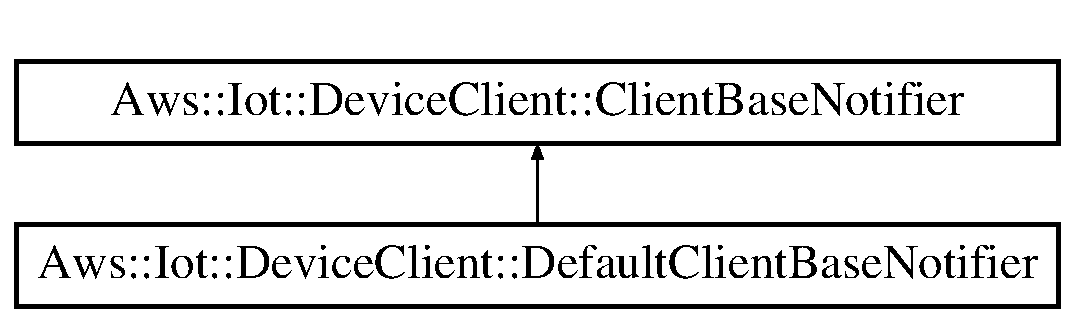
\includegraphics[height=2.000000cm]{class_aws_1_1_iot_1_1_device_client_1_1_client_base_notifier}
\end{center}
\end{figure}
\subsection*{Public Member Functions}
\begin{DoxyCompactItemize}
\item 
virtual void \hyperlink{class_aws_1_1_iot_1_1_device_client_1_1_client_base_notifier_ae892fac9b0a778d8882bf56cb88ec26d}{on\+Event} (\hyperlink{class_aws_1_1_iot_1_1_device_client_1_1_feature}{Aws\+::\+Iot\+::\+Device\+Client\+::\+Feature} $\ast$feature, Aws\+::\+Iot\+::\+Device\+Client\+::\+Client\+Base\+Event\+Notification notification)=0
\begin{DoxyCompactList}\small\item\em Indicates an event has occurred within a feature. \end{DoxyCompactList}\item 
virtual void \hyperlink{class_aws_1_1_iot_1_1_device_client_1_1_client_base_notifier_a4b1f9d16f18965cccb96de1518a53abe}{on\+Error} (\hyperlink{class_aws_1_1_iot_1_1_device_client_1_1_feature}{Aws\+::\+Iot\+::\+Device\+Client\+::\+Feature} $\ast$feature, Aws\+::\+Iot\+::\+Device\+Client\+::\+Client\+Base\+Error\+Notification notification, std\+::string message)=0
\begin{DoxyCompactList}\small\item\em Indicates an error event has occurred within a feature. \end{DoxyCompactList}\end{DoxyCompactItemize}


\subsection{Detailed Description}
Interface the provides event-\/based messaging between features and the client base (Main.\+cpp) 

This class is used to allow features to notify the client base (Main.\+cpp) of changes or events that have happened and require attention. The interface methods are implemented at the client base level, and are called upon within the feature. 

\subsection{Member Function Documentation}
\mbox{\Hypertarget{class_aws_1_1_iot_1_1_device_client_1_1_client_base_notifier_a4b1f9d16f18965cccb96de1518a53abe}\label{class_aws_1_1_iot_1_1_device_client_1_1_client_base_notifier_a4b1f9d16f18965cccb96de1518a53abe}} 
\index{Aws\+::\+Iot\+::\+Device\+Client\+::\+Client\+Base\+Notifier@{Aws\+::\+Iot\+::\+Device\+Client\+::\+Client\+Base\+Notifier}!on\+Error@{on\+Error}}
\index{on\+Error@{on\+Error}!Aws\+::\+Iot\+::\+Device\+Client\+::\+Client\+Base\+Notifier@{Aws\+::\+Iot\+::\+Device\+Client\+::\+Client\+Base\+Notifier}}
\subsubsection{\texorpdfstring{on\+Error()}{onError()}}
{\footnotesize\ttfamily virtual void Aws\+::\+Iot\+::\+Device\+Client\+::\+Client\+Base\+Notifier\+::on\+Error (\begin{DoxyParamCaption}\item[{\hyperlink{class_aws_1_1_iot_1_1_device_client_1_1_feature}{Aws\+::\+Iot\+::\+Device\+Client\+::\+Feature} $\ast$}]{feature,  }\item[{Aws\+::\+Iot\+::\+Device\+Client\+::\+Client\+Base\+Error\+Notification}]{notification,  }\item[{std\+::string}]{message }\end{DoxyParamCaption})\hspace{0.3cm}{\ttfamily [pure virtual]}}



Indicates an error event has occurred within a feature. 


\begin{DoxyParams}{Parameters}
{\em feature} & a feature should pass reference to itself to aid the client base in taking action \\
\hline
{\em notification} & the error code representing the error that has occurred \\
\hline
{\em message} & an optional message that may be passed regarding the error to provide additional context \\
\hline
\end{DoxyParams}
\mbox{\Hypertarget{class_aws_1_1_iot_1_1_device_client_1_1_client_base_notifier_ae892fac9b0a778d8882bf56cb88ec26d}\label{class_aws_1_1_iot_1_1_device_client_1_1_client_base_notifier_ae892fac9b0a778d8882bf56cb88ec26d}} 
\index{Aws\+::\+Iot\+::\+Device\+Client\+::\+Client\+Base\+Notifier@{Aws\+::\+Iot\+::\+Device\+Client\+::\+Client\+Base\+Notifier}!on\+Event@{on\+Event}}
\index{on\+Event@{on\+Event}!Aws\+::\+Iot\+::\+Device\+Client\+::\+Client\+Base\+Notifier@{Aws\+::\+Iot\+::\+Device\+Client\+::\+Client\+Base\+Notifier}}
\subsubsection{\texorpdfstring{on\+Event()}{onEvent()}}
{\footnotesize\ttfamily virtual void Aws\+::\+Iot\+::\+Device\+Client\+::\+Client\+Base\+Notifier\+::on\+Event (\begin{DoxyParamCaption}\item[{\hyperlink{class_aws_1_1_iot_1_1_device_client_1_1_feature}{Aws\+::\+Iot\+::\+Device\+Client\+::\+Feature} $\ast$}]{feature,  }\item[{Aws\+::\+Iot\+::\+Device\+Client\+::\+Client\+Base\+Event\+Notification}]{notification }\end{DoxyParamCaption})\hspace{0.3cm}{\ttfamily [pure virtual]}}



Indicates an event has occurred within a feature. 


\begin{DoxyParams}{Parameters}
{\em feature} & a feature should pass reference to itself to aid the agent base in taking action \\
\hline
{\em notification} & the event code representing the event that has occurred \\
\hline
\end{DoxyParams}


Implemented in \hyperlink{class_aws_1_1_iot_1_1_device_client_1_1_default_client_base_notifier_a78ef5a78282bedbfce408e34ebb6a542}{Aws\+::\+Iot\+::\+Device\+Client\+::\+Default\+Client\+Base\+Notifier}.



The documentation for this class was generated from the following file\+:\begin{DoxyCompactItemize}
\item 
/home/\+A\+N\+T.\+A\+M\+A\+Z\+O\+N.\+C\+O\+M/lwwilkov/\+Workspace/aws-\/iot-\/device-\/client/source/Client\+Base\+Notifier.\+h\end{DoxyCompactItemize}

\hypertarget{class_aws_1_1_iot_1_1_device_client_1_1_config}{}\doxysection{Aws\+::Iot\+::Device\+Client\+::Config Class Reference}
\label{class_aws_1_1_iot_1_1_device_client_1_1_config}\index{Aws::Iot::DeviceClient::Config@{Aws::Iot::DeviceClient::Config}}
\doxysubsection*{Public Member Functions}
\begin{DoxyCompactItemize}
\item 
\mbox{\Hypertarget{class_aws_1_1_iot_1_1_device_client_1_1_config_a04650d1df3804ca66090372c000361cd}\label{class_aws_1_1_iot_1_1_device_client_1_1_config_a04650d1df3804ca66090372c000361cd}} 
bool {\bfseries Validate\+And\+Store\+Runtime\+Config} ()
\item 
\mbox{\Hypertarget{class_aws_1_1_iot_1_1_device_client_1_1_config_aa98504ecb47adcb2b314b80c8f1126cf}\label{class_aws_1_1_iot_1_1_device_client_1_1_config_aa98504ecb47adcb2b314b80c8f1126cf}} 
bool {\bfseries Parse\+Config\+File} (const std\+::string \&file, bool is\+Runtime\+Config)
\item 
\mbox{\Hypertarget{class_aws_1_1_iot_1_1_device_client_1_1_config_a9cc6f1feb804069d5fc388064385834b}\label{class_aws_1_1_iot_1_1_device_client_1_1_config_a9cc6f1feb804069d5fc388064385834b}} 
bool {\bfseries init} (const Cli\+Args \&cli\+Args)
\end{DoxyCompactItemize}
\doxysubsection*{Static Public Member Functions}
\begin{DoxyCompactItemize}
\item 
\mbox{\Hypertarget{class_aws_1_1_iot_1_1_device_client_1_1_config_a79d6a0fcb2e082a507db7f0c610193eb}\label{class_aws_1_1_iot_1_1_device_client_1_1_config_a79d6a0fcb2e082a507db7f0c610193eb}} 
static bool {\bfseries Parse\+Cli\+Args} (int argc, char $\ast$argv\mbox{[}$\,$\mbox{]}, Cli\+Args \&cli\+Args)
\end{DoxyCompactItemize}
\doxysubsection*{Public Attributes}
\begin{DoxyCompactItemize}
\item 
\mbox{\Hypertarget{class_aws_1_1_iot_1_1_device_client_1_1_config_a6eb01a26b458b7fcc4515f8a9c721516}\label{class_aws_1_1_iot_1_1_device_client_1_1_config_a6eb01a26b458b7fcc4515f8a9c721516}} 
\mbox{\hyperlink{struct_aws_1_1_iot_1_1_device_client_1_1_plain_config}{Plain\+Config}} {\bfseries config}
\end{DoxyCompactItemize}
\doxysubsection*{Static Public Attributes}
\begin{DoxyCompactItemize}
\item 
\mbox{\Hypertarget{class_aws_1_1_iot_1_1_device_client_1_1_config_a031e68a89ae130b0e057a1bb002c88e1}\label{class_aws_1_1_iot_1_1_device_client_1_1_config_a031e68a89ae130b0e057a1bb002c88e1}} 
static constexpr char {\bfseries T\+AG} \mbox{[}$\,$\mbox{]} = \char`\"{}Config.\+cpp\char`\"{}
\item 
\mbox{\Hypertarget{class_aws_1_1_iot_1_1_device_client_1_1_config_ab371eb8d56601c1e89139b3923c8a510}\label{class_aws_1_1_iot_1_1_device_client_1_1_config_ab371eb8d56601c1e89139b3923c8a510}} 
static constexpr char {\bfseries D\+E\+F\+A\+U\+L\+T\+\_\+\+C\+O\+N\+F\+I\+G\+\_\+\+D\+IR} \mbox{[}$\,$\mbox{]} = \char`\"{}$\sim$/.aws-\/iot-\/device-\/client/\char`\"{}
\item 
\mbox{\Hypertarget{class_aws_1_1_iot_1_1_device_client_1_1_config_a26fc5b345eaf56c9ef757569b3d512d0}\label{class_aws_1_1_iot_1_1_device_client_1_1_config_a26fc5b345eaf56c9ef757569b3d512d0}} 
static constexpr char {\bfseries D\+E\+F\+A\+U\+L\+T\+\_\+\+K\+E\+Y\+\_\+\+D\+IR} \mbox{[}$\,$\mbox{]} = \char`\"{}$\sim$/.aws-\/iot-\/device-\/client/keys/\char`\"{}
\item 
\mbox{\Hypertarget{class_aws_1_1_iot_1_1_device_client_1_1_config_aff1fd25389283318f0a37563b5796448}\label{class_aws_1_1_iot_1_1_device_client_1_1_config_aff1fd25389283318f0a37563b5796448}} 
static constexpr char {\bfseries D\+E\+F\+A\+U\+L\+T\+\_\+\+C\+O\+N\+F\+I\+G\+\_\+\+F\+I\+LE} \mbox{[}$\,$\mbox{]} = \char`\"{}$\sim$/.aws-\/iot-\/device-\/client/aws-\/iot-\/device-\/client.\+conf\char`\"{}
\item 
static constexpr char {\bfseries D\+E\+F\+A\+U\+L\+T\+\_\+\+F\+L\+E\+E\+T\+\_\+\+P\+R\+O\+V\+I\+S\+I\+O\+N\+I\+N\+G\+\_\+\+R\+U\+N\+T\+I\+M\+E\+\_\+\+C\+O\+N\+F\+I\+G\+\_\+\+F\+I\+LE} \mbox{[}$\,$\mbox{]}
\item 
\mbox{\Hypertarget{class_aws_1_1_iot_1_1_device_client_1_1_config_abfeb64c428bb7ceccb5a7ed41053a736}\label{class_aws_1_1_iot_1_1_device_client_1_1_config_abfeb64c428bb7ceccb5a7ed41053a736}} 
static constexpr char {\bfseries C\+L\+I\+\_\+\+H\+E\+LP} \mbox{[}$\,$\mbox{]} = \char`\"{}-\/-\/help\char`\"{}
\item 
\mbox{\Hypertarget{class_aws_1_1_iot_1_1_device_client_1_1_config_aa68ce541f883e9f7d4777b68f2edb073}\label{class_aws_1_1_iot_1_1_device_client_1_1_config_aa68ce541f883e9f7d4777b68f2edb073}} 
static constexpr char {\bfseries C\+L\+I\+\_\+\+E\+X\+P\+O\+R\+T\+\_\+\+D\+E\+F\+A\+U\+L\+T\+\_\+\+S\+E\+T\+T\+I\+N\+GS} \mbox{[}$\,$\mbox{]} = \char`\"{}-\/-\/export-\/default-\/settings\char`\"{}
\item 
\mbox{\Hypertarget{class_aws_1_1_iot_1_1_device_client_1_1_config_a5d750b00b78159cc0d053db72498e7c7}\label{class_aws_1_1_iot_1_1_device_client_1_1_config_a5d750b00b78159cc0d053db72498e7c7}} 
static constexpr char {\bfseries C\+L\+I\+\_\+\+C\+O\+N\+F\+I\+G\+\_\+\+F\+I\+LE} \mbox{[}$\,$\mbox{]} = \char`\"{}-\/-\/config-\/file\char`\"{}
\end{DoxyCompactItemize}
\doxysubsection*{Static Private Member Functions}
\begin{DoxyCompactItemize}
\item 
\mbox{\Hypertarget{class_aws_1_1_iot_1_1_device_client_1_1_config_afd3f26a6bd9666087b85f09de007c38e}\label{class_aws_1_1_iot_1_1_device_client_1_1_config_afd3f26a6bd9666087b85f09de007c38e}} 
static void {\bfseries Print\+Help\+Message} ()
\item 
\mbox{\Hypertarget{class_aws_1_1_iot_1_1_device_client_1_1_config_a121dabe3897256fd1aece128f8f54bc7}\label{class_aws_1_1_iot_1_1_device_client_1_1_config_a121dabe3897256fd1aece128f8f54bc7}} 
static bool {\bfseries Export\+Default\+Setting} (const std\+::string \&file)
\end{DoxyCompactItemize}


\doxysubsection{Member Data Documentation}
\mbox{\Hypertarget{class_aws_1_1_iot_1_1_device_client_1_1_config_a53502fe325290f50fe2b0dd02ade46e7}\label{class_aws_1_1_iot_1_1_device_client_1_1_config_a53502fe325290f50fe2b0dd02ade46e7}} 
\index{Aws::Iot::DeviceClient::Config@{Aws::Iot::DeviceClient::Config}!DEFAULT\_FLEET\_PROVISIONING\_RUNTIME\_CONFIG\_FILE@{DEFAULT\_FLEET\_PROVISIONING\_RUNTIME\_CONFIG\_FILE}}
\index{DEFAULT\_FLEET\_PROVISIONING\_RUNTIME\_CONFIG\_FILE@{DEFAULT\_FLEET\_PROVISIONING\_RUNTIME\_CONFIG\_FILE}!Aws::Iot::DeviceClient::Config@{Aws::Iot::DeviceClient::Config}}
\doxysubsubsection{\texorpdfstring{DEFAULT\_FLEET\_PROVISIONING\_RUNTIME\_CONFIG\_FILE}{DEFAULT\_FLEET\_PROVISIONING\_RUNTIME\_CONFIG\_FILE}}
{\footnotesize\ttfamily constexpr char Config\+::\+D\+E\+F\+A\+U\+L\+T\+\_\+\+F\+L\+E\+E\+T\+\_\+\+P\+R\+O\+V\+I\+S\+I\+O\+N\+I\+N\+G\+\_\+\+R\+U\+N\+T\+I\+M\+E\+\_\+\+C\+O\+N\+F\+I\+G\+\_\+\+F\+I\+LE\hspace{0.3cm}{\ttfamily [static]}, {\ttfamily [constexpr]}}

{\bfseries Initial value\+:}
\begin{DoxyCode}{0}
\DoxyCodeLine{=}
\DoxyCodeLine{                    \textcolor{stringliteral}{"\string~/.aws-\/iot-\/device-\/client/aws-\/iot-\/device-\/client-\/runtime.conf"}}

\end{DoxyCode}


The documentation for this class was generated from the following files\+:\begin{DoxyCompactItemize}
\item 
/home/runner/work/aws-\/iot-\/device-\/client/aws-\/iot-\/device-\/client/source/config/Config.\+h\item 
/home/runner/work/aws-\/iot-\/device-\/client/aws-\/iot-\/device-\/client/source/config/Config.\+cpp\end{DoxyCompactItemize}

\hypertarget{class_aws_1_1_iot_1_1_device_client_1_1_default_client_base_notifier}{}\doxysection{Aws\+::Iot\+::Device\+Client\+::Default\+Client\+Base\+Notifier Class Reference}
\label{class_aws_1_1_iot_1_1_device_client_1_1_default_client_base_notifier}\index{Aws::Iot::DeviceClient::DefaultClientBaseNotifier@{Aws::Iot::DeviceClient::DefaultClientBaseNotifier}}


Represents the default set of behavior we expect to exhibit when receiving events from a feature.  


Inheritance diagram for Aws\+::Iot\+::Device\+Client\+::Default\+Client\+Base\+Notifier\+:\begin{figure}[H]
\begin{center}
\leavevmode
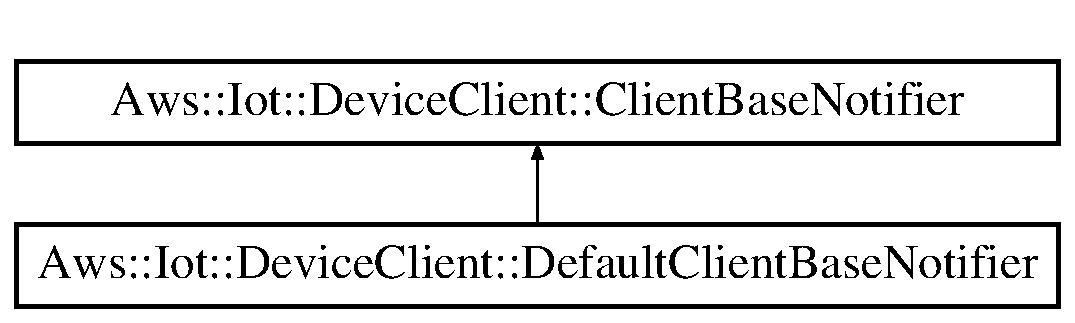
\includegraphics[height=2.000000cm]{class_aws_1_1_iot_1_1_device_client_1_1_default_client_base_notifier}
\end{center}
\end{figure}
\doxysubsection*{Private Member Functions}
\begin{DoxyCompactItemize}
\item 
void \mbox{\hyperlink{class_aws_1_1_iot_1_1_device_client_1_1_default_client_base_notifier_a78ef5a78282bedbfce408e34ebb6a542}{on\+Event}} (\mbox{\hyperlink{class_aws_1_1_iot_1_1_device_client_1_1_feature}{Feature}} $\ast$feature, Client\+Base\+Event\+Notification notification)
\begin{DoxyCompactList}\small\item\em Indicates an event has occurred within a feature. \end{DoxyCompactList}\item 
\mbox{\Hypertarget{class_aws_1_1_iot_1_1_device_client_1_1_default_client_base_notifier_aaff465fc5084f8fe6de4c7362a8e49fb}\label{class_aws_1_1_iot_1_1_device_client_1_1_default_client_base_notifier_aaff465fc5084f8fe6de4c7362a8e49fb}} 
void {\bfseries on\+Error} (\mbox{\hyperlink{class_aws_1_1_iot_1_1_device_client_1_1_feature}{Feature}} $\ast$feature, Client\+Base\+Error\+Notification error, string msg)
\end{DoxyCompactItemize}
\doxysubsection*{Additional Inherited Members}


\doxysubsection{Detailed Description}
Represents the default set of behavior we expect to exhibit when receiving events from a feature. 

\doxysubsection{Member Function Documentation}
\mbox{\Hypertarget{class_aws_1_1_iot_1_1_device_client_1_1_default_client_base_notifier_a78ef5a78282bedbfce408e34ebb6a542}\label{class_aws_1_1_iot_1_1_device_client_1_1_default_client_base_notifier_a78ef5a78282bedbfce408e34ebb6a542}} 
\index{Aws::Iot::DeviceClient::DefaultClientBaseNotifier@{Aws::Iot::DeviceClient::DefaultClientBaseNotifier}!onEvent@{onEvent}}
\index{onEvent@{onEvent}!Aws::Iot::DeviceClient::DefaultClientBaseNotifier@{Aws::Iot::DeviceClient::DefaultClientBaseNotifier}}
\doxysubsubsection{\texorpdfstring{onEvent()}{onEvent()}}
{\footnotesize\ttfamily void Aws\+::\+Iot\+::\+Device\+Client\+::\+Default\+Client\+Base\+Notifier\+::on\+Event (\begin{DoxyParamCaption}\item[{\mbox{\hyperlink{class_aws_1_1_iot_1_1_device_client_1_1_feature}{Feature}} $\ast$}]{feature,  }\item[{Client\+Base\+Event\+Notification}]{notification }\end{DoxyParamCaption})\hspace{0.3cm}{\ttfamily [inline]}, {\ttfamily [private]}, {\ttfamily [virtual]}}



Indicates an event has occurred within a feature. 


\begin{DoxyParams}{Parameters}
{\em feature} & a feature should pass reference to itself to aid the agent base in taking action \\
\hline
{\em notification} & the event code representing the event that has occurred \\
\hline
\end{DoxyParams}


Implements \mbox{\hyperlink{class_aws_1_1_iot_1_1_device_client_1_1_client_base_notifier_ae892fac9b0a778d8882bf56cb88ec26d}{Aws\+::\+Iot\+::\+Device\+Client\+::\+Client\+Base\+Notifier}}.



The documentation for this class was generated from the following file\+:\begin{DoxyCompactItemize}
\item 
/home/runner/work/aws-\/iot-\/device-\/client/aws-\/iot-\/device-\/client/source/main.\+cpp\end{DoxyCompactItemize}

\hypertarget{struct_aws_1_1_iot_1_1_device_client_1_1_plain_config_1_1_device_defender}{}\section{Aws\+:\+:Iot\+:\+:Device\+Client\+:\+:Plain\+Config\+:\+:Device\+Defender Struct Reference}
\label{struct_aws_1_1_iot_1_1_device_client_1_1_plain_config_1_1_device_defender}\index{Aws\+::\+Iot\+::\+Device\+Client\+::\+Plain\+Config\+::\+Device\+Defender@{Aws\+::\+Iot\+::\+Device\+Client\+::\+Plain\+Config\+::\+Device\+Defender}}
Inheritance diagram for Aws\+:\+:Iot\+:\+:Device\+Client\+:\+:Plain\+Config\+:\+:Device\+Defender\+:\begin{figure}[H]
\begin{center}
\leavevmode
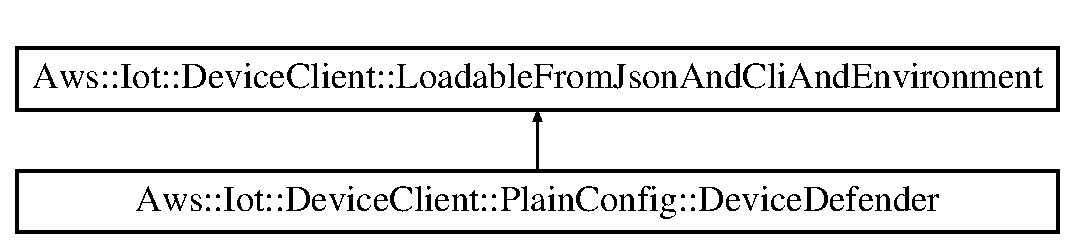
\includegraphics[height=2.000000cm]{struct_aws_1_1_iot_1_1_device_client_1_1_plain_config_1_1_device_defender}
\end{center}
\end{figure}
\subsection*{Public Member Functions}
\begin{DoxyCompactItemize}
\item 
\mbox{\Hypertarget{struct_aws_1_1_iot_1_1_device_client_1_1_plain_config_1_1_device_defender_a03e9f5cb08c3e3dd87629488df9a15c2}\label{struct_aws_1_1_iot_1_1_device_client_1_1_plain_config_1_1_device_defender_a03e9f5cb08c3e3dd87629488df9a15c2}} 
bool {\bfseries Load\+From\+Json} (const Crt\+::\+Json\+View \&json) override
\item 
\mbox{\Hypertarget{struct_aws_1_1_iot_1_1_device_client_1_1_plain_config_1_1_device_defender_a26abac0d7ba9adbbe28ed43252b68268}\label{struct_aws_1_1_iot_1_1_device_client_1_1_plain_config_1_1_device_defender_a26abac0d7ba9adbbe28ed43252b68268}} 
bool {\bfseries Load\+From\+Cli\+Args} (const Cli\+Args \&cli\+Args) override
\item 
\mbox{\Hypertarget{struct_aws_1_1_iot_1_1_device_client_1_1_plain_config_1_1_device_defender_a0f48a02304ceb73f818b9386211d1244}\label{struct_aws_1_1_iot_1_1_device_client_1_1_plain_config_1_1_device_defender_a0f48a02304ceb73f818b9386211d1244}} 
bool {\bfseries Load\+From\+Environment} () override
\item 
\mbox{\Hypertarget{struct_aws_1_1_iot_1_1_device_client_1_1_plain_config_1_1_device_defender_ad157a10deb0fef6762d9a4283c3f00e3}\label{struct_aws_1_1_iot_1_1_device_client_1_1_plain_config_1_1_device_defender_ad157a10deb0fef6762d9a4283c3f00e3}} 
bool {\bfseries Validate} () const override
\end{DoxyCompactItemize}
\subsection*{Public Attributes}
\begin{DoxyCompactItemize}
\item 
\mbox{\Hypertarget{struct_aws_1_1_iot_1_1_device_client_1_1_plain_config_1_1_device_defender_ad1be4257e9cabc30f3d328fd5a968099}\label{struct_aws_1_1_iot_1_1_device_client_1_1_plain_config_1_1_device_defender_ad1be4257e9cabc30f3d328fd5a968099}} 
bool {\bfseries enabled} \{true\}
\item 
\mbox{\Hypertarget{struct_aws_1_1_iot_1_1_device_client_1_1_plain_config_1_1_device_defender_a1407a25d4b3bacbd0578339eb0847db0}\label{struct_aws_1_1_iot_1_1_device_client_1_1_plain_config_1_1_device_defender_a1407a25d4b3bacbd0578339eb0847db0}} 
int {\bfseries interval} \{300\}
\end{DoxyCompactItemize}
\subsection*{Static Public Attributes}
\begin{DoxyCompactItemize}
\item 
\mbox{\Hypertarget{struct_aws_1_1_iot_1_1_device_client_1_1_plain_config_1_1_device_defender_a61696ee467defb358e58621a16eb7b07}\label{struct_aws_1_1_iot_1_1_device_client_1_1_plain_config_1_1_device_defender_a61696ee467defb358e58621a16eb7b07}} 
static constexpr char {\bfseries C\+L\+I\+\_\+\+E\+N\+A\+B\+L\+E\+\_\+\+D\+E\+V\+I\+C\+E\+\_\+\+D\+E\+F\+E\+N\+D\+ER} \mbox{[}$\,$\mbox{]} = \char`\"{}-\/-\/enable-\/device-\/defender\char`\"{}
\item 
\mbox{\Hypertarget{struct_aws_1_1_iot_1_1_device_client_1_1_plain_config_1_1_device_defender_a4e7ed3859ac73100a22e4d89bf540f8d}\label{struct_aws_1_1_iot_1_1_device_client_1_1_plain_config_1_1_device_defender_a4e7ed3859ac73100a22e4d89bf540f8d}} 
static constexpr char {\bfseries C\+L\+I\+\_\+\+D\+E\+V\+I\+C\+E\+\_\+\+D\+E\+F\+E\+N\+D\+E\+R\+\_\+\+I\+N\+T\+E\+R\+V\+AL} \mbox{[}$\,$\mbox{]} = \char`\"{}-\/-\/device-\/defender-\/interval\char`\"{}
\item 
\mbox{\Hypertarget{struct_aws_1_1_iot_1_1_device_client_1_1_plain_config_1_1_device_defender_af35ebcc9d16004b8aaadf5405b0213a4}\label{struct_aws_1_1_iot_1_1_device_client_1_1_plain_config_1_1_device_defender_af35ebcc9d16004b8aaadf5405b0213a4}} 
static constexpr char {\bfseries J\+S\+O\+N\+\_\+\+K\+E\+Y\+\_\+\+E\+N\+A\+B\+L\+ED} \mbox{[}$\,$\mbox{]} = \char`\"{}enabled\char`\"{}
\item 
\mbox{\Hypertarget{struct_aws_1_1_iot_1_1_device_client_1_1_plain_config_1_1_device_defender_a19b3d056cf398072d11484499ba36f59}\label{struct_aws_1_1_iot_1_1_device_client_1_1_plain_config_1_1_device_defender_a19b3d056cf398072d11484499ba36f59}} 
static constexpr char {\bfseries J\+S\+O\+N\+\_\+\+K\+E\+Y\+\_\+\+I\+N\+T\+E\+R\+V\+AL} \mbox{[}$\,$\mbox{]} = \char`\"{}interval-\/in-\/seconds\char`\"{}
\end{DoxyCompactItemize}


The documentation for this struct was generated from the following files\+:\begin{DoxyCompactItemize}
\item 
/home/\+A\+N\+T.\+A\+M\+A\+Z\+O\+N.\+C\+O\+M/lwwilkov/\+Workspace/aws-\/iot-\/device-\/client/source/config/Config.\+h\item 
/home/\+A\+N\+T.\+A\+M\+A\+Z\+O\+N.\+C\+O\+M/lwwilkov/\+Workspace/aws-\/iot-\/device-\/client/source/config/Config.\+cpp\end{DoxyCompactItemize}

\hypertarget{class_aws_1_1_iot_1_1_device_client_1_1_device_defender_1_1_device_defender_feature}{}\section{Aws\+:\+:Iot\+:\+:Device\+Client\+:\+:Device\+Defender\+:\+:Device\+Defender\+Feature Class Reference}
\label{class_aws_1_1_iot_1_1_device_client_1_1_device_defender_1_1_device_defender_feature}\index{Aws\+::\+Iot\+::\+Device\+Client\+::\+Device\+Defender\+::\+Device\+Defender\+Feature@{Aws\+::\+Iot\+::\+Device\+Client\+::\+Device\+Defender\+::\+Device\+Defender\+Feature}}


Provides IoT Device Defender related functionality within the Device Client.  




{\ttfamily \#include $<$Device\+Defender\+Feature.\+h$>$}

Inheritance diagram for Aws\+:\+:Iot\+:\+:Device\+Client\+:\+:Device\+Defender\+:\+:Device\+Defender\+Feature\+:\begin{figure}[H]
\begin{center}
\leavevmode
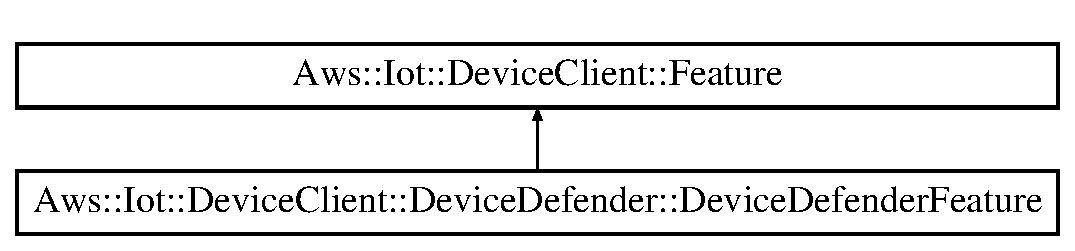
\includegraphics[height=2.000000cm]{class_aws_1_1_iot_1_1_device_client_1_1_device_defender_1_1_device_defender_feature}
\end{center}
\end{figure}
\subsection*{Public Member Functions}
\begin{DoxyCompactItemize}
\item 
int \hyperlink{class_aws_1_1_iot_1_1_device_client_1_1_device_defender_1_1_device_defender_feature_a7fe61ca792baf877da7bbbd00e81629b}{init} (std\+::shared\+\_\+ptr$<$ \hyperlink{class_aws_1_1_iot_1_1_device_client_1_1_shared_crt_resource_manager}{Shared\+Crt\+Resource\+Manager} $>$ manager, std\+::shared\+\_\+ptr$<$ \hyperlink{class_aws_1_1_iot_1_1_device_client_1_1_client_base_notifier}{Client\+Base\+Notifier} $>$ notifier, const \hyperlink{struct_aws_1_1_iot_1_1_device_client_1_1_plain_config}{Plain\+Config} \&config)
\begin{DoxyCompactList}\small\item\em Initializes the Device Defender feature with all the required setup information, event handlers, and the shared Mqtt\+Connection. \end{DoxyCompactList}\item 
\mbox{\Hypertarget{class_aws_1_1_iot_1_1_device_client_1_1_device_defender_1_1_device_defender_feature_a9756456b46159446a17e93d65028963b}\label{class_aws_1_1_iot_1_1_device_client_1_1_device_defender_1_1_device_defender_feature_a9756456b46159446a17e93d65028963b}} 
void {\bfseries Load\+From\+Config} (const \hyperlink{struct_aws_1_1_iot_1_1_device_client_1_1_plain_config}{Plain\+Config} \&config)
\item 
std\+::string \hyperlink{class_aws_1_1_iot_1_1_device_client_1_1_device_defender_1_1_device_defender_feature_a5d1c425fb35d74caff528e7b59026211}{get\+Name} () override
\begin{DoxyCompactList}\small\item\em For a given feature, returns its name. \end{DoxyCompactList}\item 
int \hyperlink{class_aws_1_1_iot_1_1_device_client_1_1_device_defender_1_1_device_defender_feature_aeede868840f237a50d394c779a8a9026}{start} () override
\begin{DoxyCompactList}\small\item\em Start the feature. \end{DoxyCompactList}\item 
int \hyperlink{class_aws_1_1_iot_1_1_device_client_1_1_device_defender_1_1_device_defender_feature_a93b78c0fe8518baabdff3d38544b9d00}{stop} () override
\begin{DoxyCompactList}\small\item\em Stop the feature. \end{DoxyCompactList}\end{DoxyCompactItemize}
\subsection*{Private Member Functions}
\begin{DoxyCompactItemize}
\item 
\mbox{\Hypertarget{class_aws_1_1_iot_1_1_device_client_1_1_device_defender_1_1_device_defender_feature_a0d3be7affd06c7e2527f382a18a41faf}\label{class_aws_1_1_iot_1_1_device_client_1_1_device_defender_1_1_device_defender_feature_a0d3be7affd06c7e2527f382a18a41faf}} 
void \hyperlink{class_aws_1_1_iot_1_1_device_client_1_1_device_defender_1_1_device_defender_feature_a0d3be7affd06c7e2527f382a18a41faf}{start\+Device\+Defender} ()
\begin{DoxyCompactList}\small\item\em Called by feature start, this will build the task, add it to the event\+Loop\+Group in the \hyperlink{class_aws_1_1_iot_1_1_device_client_1_1_shared_crt_resource_manager}{Shared\+Crt\+Resource\+Manager}, \& will start the task. This function will also subscribe to the accepted/rejected Device Defender M\+Q\+TT topics. \end{DoxyCompactList}\item 
\mbox{\Hypertarget{class_aws_1_1_iot_1_1_device_client_1_1_device_defender_1_1_device_defender_feature_ad6b99bdbb2c41252cdfb9c8ae6315bb7}\label{class_aws_1_1_iot_1_1_device_client_1_1_device_defender_1_1_device_defender_feature_ad6b99bdbb2c41252cdfb9c8ae6315bb7}} 
void \hyperlink{class_aws_1_1_iot_1_1_device_client_1_1_device_defender_1_1_device_defender_feature_ad6b99bdbb2c41252cdfb9c8ae6315bb7}{stop\+Device\+Defender} ()
\begin{DoxyCompactList}\small\item\em Called when Iot Device Defender S\+DK task stops, this function will stop the Iot Device Defender S\+DK task, \& unsubscribe from the accepted/rejected Device Defender M\+Q\+TT topics. \end{DoxyCompactList}\end{DoxyCompactItemize}
\subsection*{Private Attributes}
\begin{DoxyCompactItemize}
\item 
\mbox{\Hypertarget{class_aws_1_1_iot_1_1_device_client_1_1_device_defender_1_1_device_defender_feature_ac3e35348cde1d5d6a9f0d94d401c5be8}\label{class_aws_1_1_iot_1_1_device_client_1_1_device_defender_1_1_device_defender_feature_ac3e35348cde1d5d6a9f0d94d401c5be8}} 
int \hyperlink{class_aws_1_1_iot_1_1_device_client_1_1_device_defender_1_1_device_defender_feature_ac3e35348cde1d5d6a9f0d94d401c5be8}{interval}
\begin{DoxyCompactList}\small\item\em An interval in seconds used to determine how often to publish reports. \end{DoxyCompactList}\item 
\mbox{\Hypertarget{class_aws_1_1_iot_1_1_device_client_1_1_device_defender_1_1_device_defender_feature_a94c232fb069b691c86f50e071be52980}\label{class_aws_1_1_iot_1_1_device_client_1_1_device_defender_1_1_device_defender_feature_a94c232fb069b691c86f50e071be52980}} 
std\+::string \hyperlink{class_aws_1_1_iot_1_1_device_client_1_1_device_defender_1_1_device_defender_feature_a94c232fb069b691c86f50e071be52980}{thing\+Name}
\begin{DoxyCompactList}\small\item\em the Thing\+Name to use \end{DoxyCompactList}\item 
\mbox{\Hypertarget{class_aws_1_1_iot_1_1_device_client_1_1_device_defender_1_1_device_defender_feature_abe2e798db9d8c78b478441cb95f0ca15}\label{class_aws_1_1_iot_1_1_device_client_1_1_device_defender_1_1_device_defender_feature_abe2e798db9d8c78b478441cb95f0ca15}} 
std\+::shared\+\_\+ptr$<$ \hyperlink{class_aws_1_1_iot_1_1_device_client_1_1_shared_crt_resource_manager}{Shared\+Crt\+Resource\+Manager} $>$ \hyperlink{class_aws_1_1_iot_1_1_device_client_1_1_device_defender_1_1_device_defender_feature_abe2e798db9d8c78b478441cb95f0ca15}{resource\+Manager}
\begin{DoxyCompactList}\small\item\em The resource manager used to manage C\+RT resources. \end{DoxyCompactList}\item 
\mbox{\Hypertarget{class_aws_1_1_iot_1_1_device_client_1_1_device_defender_1_1_device_defender_feature_aa2f55fc2a35b656301cf0039f09bc408}\label{class_aws_1_1_iot_1_1_device_client_1_1_device_defender_1_1_device_defender_feature_aa2f55fc2a35b656301cf0039f09bc408}} 
std\+::shared\+\_\+ptr$<$ \hyperlink{class_aws_1_1_iot_1_1_device_client_1_1_client_base_notifier}{Client\+Base\+Notifier} $>$ \hyperlink{class_aws_1_1_iot_1_1_device_client_1_1_device_defender_1_1_device_defender_feature_aa2f55fc2a35b656301cf0039f09bc408}{base\+Notifier}
\begin{DoxyCompactList}\small\item\em An interface used to notify the Client base if there is an event that requires its attention. \end{DoxyCompactList}\item 
\mbox{\Hypertarget{class_aws_1_1_iot_1_1_device_client_1_1_device_defender_1_1_device_defender_feature_a76a601d0e3709a5984e7922721a30619}\label{class_aws_1_1_iot_1_1_device_client_1_1_device_defender_1_1_device_defender_feature_a76a601d0e3709a5984e7922721a30619}} 
std\+::unique\+\_\+ptr$<$ Aws\+::\+Iotdevicedefenderv1\+::\+Report\+Task $>$ \hyperlink{class_aws_1_1_iot_1_1_device_client_1_1_device_defender_1_1_device_defender_feature_a76a601d0e3709a5984e7922721a30619}{task}
\begin{DoxyCompactList}\small\item\em The Iot Device Defender S\+DK task responsible for publishing the reports. \end{DoxyCompactList}\end{DoxyCompactItemize}
\subsection*{Static Private Attributes}
\begin{DoxyCompactItemize}
\item 
\mbox{\Hypertarget{class_aws_1_1_iot_1_1_device_client_1_1_device_defender_1_1_device_defender_feature_a418d69418549311e3026386766ca6638}\label{class_aws_1_1_iot_1_1_device_client_1_1_device_defender_1_1_device_defender_feature_a418d69418549311e3026386766ca6638}} 
static constexpr char \hyperlink{class_aws_1_1_iot_1_1_device_client_1_1_device_defender_1_1_device_defender_feature_a418d69418549311e3026386766ca6638}{T\+AG} \mbox{[}$\,$\mbox{]} = \char`\"{}Device\+Defender.\+cpp\char`\"{}
\begin{DoxyCompactList}\small\item\em Used by the logger to specify that log messages are coming from the Device Defender feature. \end{DoxyCompactList}\item 
\mbox{\Hypertarget{class_aws_1_1_iot_1_1_device_client_1_1_device_defender_1_1_device_defender_feature_a184874a29b7c367e898ec386fff1a83f}\label{class_aws_1_1_iot_1_1_device_client_1_1_device_defender_1_1_device_defender_feature_a184874a29b7c367e898ec386fff1a83f}} 
static constexpr char \hyperlink{class_aws_1_1_iot_1_1_device_client_1_1_device_defender_1_1_device_defender_feature_a184874a29b7c367e898ec386fff1a83f}{T\+O\+P\+I\+C\+\_\+\+P\+RE} \mbox{[}$\,$\mbox{]} = \char`\"{}\$aws/things/\char`\"{}
\begin{DoxyCompactList}\small\item\em The first part of the M\+Q\+TT topic that is built around the thing\+Name, \$aws/things/$<$thing\+Name$>$/defender/metrics/json. \end{DoxyCompactList}\item 
\mbox{\Hypertarget{class_aws_1_1_iot_1_1_device_client_1_1_device_defender_1_1_device_defender_feature_ab6407a1677ee82a399fa6ab04fdcaeac}\label{class_aws_1_1_iot_1_1_device_client_1_1_device_defender_1_1_device_defender_feature_ab6407a1677ee82a399fa6ab04fdcaeac}} 
static constexpr char \hyperlink{class_aws_1_1_iot_1_1_device_client_1_1_device_defender_1_1_device_defender_feature_ab6407a1677ee82a399fa6ab04fdcaeac}{T\+O\+P\+I\+C\+\_\+\+P\+O\+ST} \mbox{[}$\,$\mbox{]} = \char`\"{}/defender/metrics/json\char`\"{}
\begin{DoxyCompactList}\small\item\em The second part of the M\+Q\+TT topic that is built around the thing\+Name, \$aws/things/$<$thing\+Name$>$/defender/metrics/json. \end{DoxyCompactList}\item 
\mbox{\Hypertarget{class_aws_1_1_iot_1_1_device_client_1_1_device_defender_1_1_device_defender_feature_a126efcfab79ced5cf92f19075cc783c8}\label{class_aws_1_1_iot_1_1_device_client_1_1_device_defender_1_1_device_defender_feature_a126efcfab79ced5cf92f19075cc783c8}} 
static constexpr char \hyperlink{class_aws_1_1_iot_1_1_device_client_1_1_device_defender_1_1_device_defender_feature_a126efcfab79ced5cf92f19075cc783c8}{T\+O\+P\+I\+C\+\_\+\+A\+C\+C\+E\+P\+T\+ED} \mbox{[}$\,$\mbox{]} = \char`\"{}/accepted\char`\"{}
\begin{DoxyCompactList}\small\item\em The third part of the M\+Q\+TT topic that is built around the thing\+Name published to by the service when reports are accepted. \$aws/things/$<$thing\+Name$>$/defender/metrics/json/accepted. \end{DoxyCompactList}\item 
\mbox{\Hypertarget{class_aws_1_1_iot_1_1_device_client_1_1_device_defender_1_1_device_defender_feature_aed0c10562d74c6232c5450a8fa608ea5}\label{class_aws_1_1_iot_1_1_device_client_1_1_device_defender_1_1_device_defender_feature_aed0c10562d74c6232c5450a8fa608ea5}} 
static constexpr char \hyperlink{class_aws_1_1_iot_1_1_device_client_1_1_device_defender_1_1_device_defender_feature_aed0c10562d74c6232c5450a8fa608ea5}{T\+O\+P\+I\+C\+\_\+\+R\+E\+J\+E\+C\+T\+ED} \mbox{[}$\,$\mbox{]} = \char`\"{}/rejected\char`\"{}
\begin{DoxyCompactList}\small\item\em The third part of the M\+Q\+TT topic that is built around the thing\+Name published to by the service when reports are rejected \$aws/things/$<$thing\+Name$>$/defender/metrics/json/rejected. \end{DoxyCompactList}\end{DoxyCompactItemize}


\subsection{Detailed Description}
Provides IoT Device Defender related functionality within the Device Client. 

\subsection{Member Function Documentation}
\mbox{\Hypertarget{class_aws_1_1_iot_1_1_device_client_1_1_device_defender_1_1_device_defender_feature_a5d1c425fb35d74caff528e7b59026211}\label{class_aws_1_1_iot_1_1_device_client_1_1_device_defender_1_1_device_defender_feature_a5d1c425fb35d74caff528e7b59026211}} 
\index{Aws\+::\+Iot\+::\+Device\+Client\+::\+Device\+Defender\+::\+Device\+Defender\+Feature@{Aws\+::\+Iot\+::\+Device\+Client\+::\+Device\+Defender\+::\+Device\+Defender\+Feature}!get\+Name@{get\+Name}}
\index{get\+Name@{get\+Name}!Aws\+::\+Iot\+::\+Device\+Client\+::\+Device\+Defender\+::\+Device\+Defender\+Feature@{Aws\+::\+Iot\+::\+Device\+Client\+::\+Device\+Defender\+::\+Device\+Defender\+Feature}}
\subsubsection{\texorpdfstring{get\+Name()}{getName()}}
{\footnotesize\ttfamily string Aws\+::\+Iot\+::\+Device\+Client\+::\+Device\+Defender\+::\+Device\+Defender\+Feature\+::get\+Name (\begin{DoxyParamCaption}{ }\end{DoxyParamCaption})\hspace{0.3cm}{\ttfamily [override]}, {\ttfamily [virtual]}}



For a given feature, returns its name. 

\begin{DoxyReturn}{Returns}
a string value representing the feature\textquotesingle{}s name 
\end{DoxyReturn}


Implements \hyperlink{class_aws_1_1_iot_1_1_device_client_1_1_feature_a7f56b81457898d67ddc1942e57e3c0d5}{Aws\+::\+Iot\+::\+Device\+Client\+::\+Feature}.

\mbox{\Hypertarget{class_aws_1_1_iot_1_1_device_client_1_1_device_defender_1_1_device_defender_feature_a7fe61ca792baf877da7bbbd00e81629b}\label{class_aws_1_1_iot_1_1_device_client_1_1_device_defender_1_1_device_defender_feature_a7fe61ca792baf877da7bbbd00e81629b}} 
\index{Aws\+::\+Iot\+::\+Device\+Client\+::\+Device\+Defender\+::\+Device\+Defender\+Feature@{Aws\+::\+Iot\+::\+Device\+Client\+::\+Device\+Defender\+::\+Device\+Defender\+Feature}!init@{init}}
\index{init@{init}!Aws\+::\+Iot\+::\+Device\+Client\+::\+Device\+Defender\+::\+Device\+Defender\+Feature@{Aws\+::\+Iot\+::\+Device\+Client\+::\+Device\+Defender\+::\+Device\+Defender\+Feature}}
\subsubsection{\texorpdfstring{init()}{init()}}
{\footnotesize\ttfamily int Aws\+::\+Iot\+::\+Device\+Client\+::\+Device\+Defender\+::\+Device\+Defender\+Feature\+::init (\begin{DoxyParamCaption}\item[{std\+::shared\+\_\+ptr$<$ \hyperlink{class_aws_1_1_iot_1_1_device_client_1_1_shared_crt_resource_manager}{Shared\+Crt\+Resource\+Manager} $>$}]{manager,  }\item[{std\+::shared\+\_\+ptr$<$ \hyperlink{class_aws_1_1_iot_1_1_device_client_1_1_client_base_notifier}{Client\+Base\+Notifier} $>$}]{notifier,  }\item[{const \hyperlink{struct_aws_1_1_iot_1_1_device_client_1_1_plain_config}{Plain\+Config} \&}]{config }\end{DoxyParamCaption})}



Initializes the Device Defender feature with all the required setup information, event handlers, and the shared Mqtt\+Connection. 


\begin{DoxyParams}{Parameters}
{\em manager} & the shared Mqtt\+Connection\+Manager \\
\hline
{\em notifier} & an \hyperlink{class_aws_1_1_iot_1_1_device_client_1_1_client_base_notifier}{Client\+Base\+Notifier} used for notifying the client base of events or errors \\
\hline
{\em config} & configuration information passed in by the user via either the command line or configuration file \\
\hline
\end{DoxyParams}
\begin{DoxyReturn}{Returns}
a non-\/zero return code indicates a problem. The logs can be checked for more info 
\end{DoxyReturn}
\mbox{\Hypertarget{class_aws_1_1_iot_1_1_device_client_1_1_device_defender_1_1_device_defender_feature_aeede868840f237a50d394c779a8a9026}\label{class_aws_1_1_iot_1_1_device_client_1_1_device_defender_1_1_device_defender_feature_aeede868840f237a50d394c779a8a9026}} 
\index{Aws\+::\+Iot\+::\+Device\+Client\+::\+Device\+Defender\+::\+Device\+Defender\+Feature@{Aws\+::\+Iot\+::\+Device\+Client\+::\+Device\+Defender\+::\+Device\+Defender\+Feature}!start@{start}}
\index{start@{start}!Aws\+::\+Iot\+::\+Device\+Client\+::\+Device\+Defender\+::\+Device\+Defender\+Feature@{Aws\+::\+Iot\+::\+Device\+Client\+::\+Device\+Defender\+::\+Device\+Defender\+Feature}}
\subsubsection{\texorpdfstring{start()}{start()}}
{\footnotesize\ttfamily int Aws\+::\+Iot\+::\+Device\+Client\+::\+Device\+Defender\+::\+Device\+Defender\+Feature\+::start (\begin{DoxyParamCaption}{ }\end{DoxyParamCaption})\hspace{0.3cm}{\ttfamily [override]}, {\ttfamily [virtual]}}



Start the feature. 

\begin{DoxyReturn}{Returns}
an integer representing the S\+U\+C\+C\+E\+SS or F\+A\+I\+L\+U\+RE of the \hyperlink{class_aws_1_1_iot_1_1_device_client_1_1_device_defender_1_1_device_defender_feature_aeede868840f237a50d394c779a8a9026}{start()} operation on the feature 
\end{DoxyReturn}


Implements \hyperlink{class_aws_1_1_iot_1_1_device_client_1_1_feature_ac9a936ebd88f7e35914a6aac99badf7d}{Aws\+::\+Iot\+::\+Device\+Client\+::\+Feature}.

\mbox{\Hypertarget{class_aws_1_1_iot_1_1_device_client_1_1_device_defender_1_1_device_defender_feature_a93b78c0fe8518baabdff3d38544b9d00}\label{class_aws_1_1_iot_1_1_device_client_1_1_device_defender_1_1_device_defender_feature_a93b78c0fe8518baabdff3d38544b9d00}} 
\index{Aws\+::\+Iot\+::\+Device\+Client\+::\+Device\+Defender\+::\+Device\+Defender\+Feature@{Aws\+::\+Iot\+::\+Device\+Client\+::\+Device\+Defender\+::\+Device\+Defender\+Feature}!stop@{stop}}
\index{stop@{stop}!Aws\+::\+Iot\+::\+Device\+Client\+::\+Device\+Defender\+::\+Device\+Defender\+Feature@{Aws\+::\+Iot\+::\+Device\+Client\+::\+Device\+Defender\+::\+Device\+Defender\+Feature}}
\subsubsection{\texorpdfstring{stop()}{stop()}}
{\footnotesize\ttfamily int Aws\+::\+Iot\+::\+Device\+Client\+::\+Device\+Defender\+::\+Device\+Defender\+Feature\+::stop (\begin{DoxyParamCaption}{ }\end{DoxyParamCaption})\hspace{0.3cm}{\ttfamily [override]}, {\ttfamily [virtual]}}



Stop the feature. 

\begin{DoxyReturn}{Returns}
an integer representing the S\+U\+C\+C\+E\+SS or F\+A\+I\+L\+U\+RE of the \hyperlink{class_aws_1_1_iot_1_1_device_client_1_1_device_defender_1_1_device_defender_feature_a93b78c0fe8518baabdff3d38544b9d00}{stop()} operation on the feature 
\end{DoxyReturn}


Implements \hyperlink{class_aws_1_1_iot_1_1_device_client_1_1_feature_a5b672f7b1403512cad9104ba923fc73d}{Aws\+::\+Iot\+::\+Device\+Client\+::\+Feature}.



The documentation for this class was generated from the following files\+:\begin{DoxyCompactItemize}
\item 
/home/\+A\+N\+T.\+A\+M\+A\+Z\+O\+N.\+C\+O\+M/lwwilkov/\+Workspace/aws-\/iot-\/device-\/client/source/devicedefender/Device\+Defender\+Feature.\+h\item 
/home/\+A\+N\+T.\+A\+M\+A\+Z\+O\+N.\+C\+O\+M/lwwilkov/\+Workspace/aws-\/iot-\/device-\/client/source/devicedefender/Device\+Defender\+Feature.\+cpp\end{DoxyCompactItemize}

\hypertarget{class_aws_1_1_iot_1_1_device_client_1_1_jobs_1_1_ephemeral_promise}{}\section{Aws\+:\+:Iot\+:\+:Device\+Client\+:\+:Jobs\+:\+:Ephemeral\+Promise$<$ T $>$ Class Template Reference}
\label{class_aws_1_1_iot_1_1_device_client_1_1_jobs_1_1_ephemeral_promise}\index{Aws\+::\+Iot\+::\+Device\+Client\+::\+Jobs\+::\+Ephemeral\+Promise$<$ T $>$@{Aws\+::\+Iot\+::\+Device\+Client\+::\+Jobs\+::\+Ephemeral\+Promise$<$ T $>$}}


Provides the ability to specify a point of expiration for a promise.  




{\ttfamily \#include $<$Ephemeral\+Promise.\+h$>$}

Inheritance diagram for Aws\+:\+:Iot\+:\+:Device\+Client\+:\+:Jobs\+:\+:Ephemeral\+Promise$<$ T $>$\+:\begin{figure}[H]
\begin{center}
\leavevmode
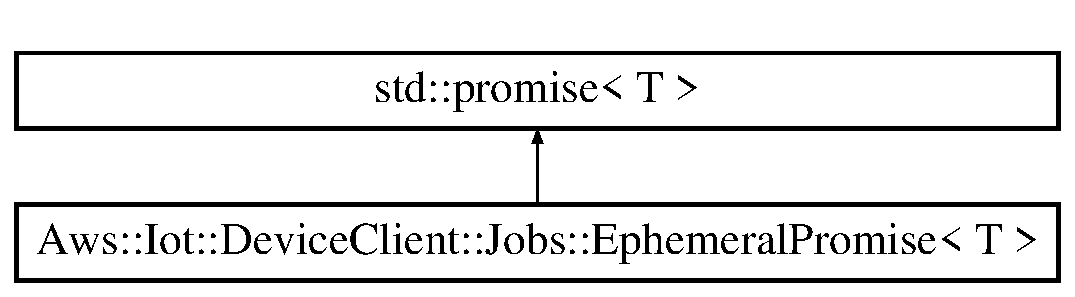
\includegraphics[height=2.000000cm]{class_aws_1_1_iot_1_1_device_client_1_1_jobs_1_1_ephemeral_promise}
\end{center}
\end{figure}
\subsection*{Public Member Functions}
\begin{DoxyCompactItemize}
\item 
\mbox{\Hypertarget{class_aws_1_1_iot_1_1_device_client_1_1_jobs_1_1_ephemeral_promise_a8dedc29ad89c996bafb0a7ea52941967}\label{class_aws_1_1_iot_1_1_device_client_1_1_jobs_1_1_ephemeral_promise_a8dedc29ad89c996bafb0a7ea52941967}} 
{\bfseries Ephemeral\+Promise} (std\+::chrono\+::milliseconds \hyperlink{class_aws_1_1_iot_1_1_device_client_1_1_jobs_1_1_ephemeral_promise_a3cd168edb7d7de52f978aa6b431ae8c0}{ttl\+Millis})
\item 
bool \hyperlink{class_aws_1_1_iot_1_1_device_client_1_1_jobs_1_1_ephemeral_promise_a4cdc9ca2aaf0aac6a397a1e2a9214c90}{is\+Expired} () const
\begin{DoxyCompactList}\small\item\em Whether the \hyperlink{class_aws_1_1_iot_1_1_device_client_1_1_jobs_1_1_ephemeral_promise}{Ephemeral\+Promise} is expired or not. \end{DoxyCompactList}\end{DoxyCompactItemize}
\subsection*{Private Member Functions}
\begin{DoxyCompactItemize}
\item 
\mbox{\Hypertarget{class_aws_1_1_iot_1_1_device_client_1_1_jobs_1_1_ephemeral_promise_aed6485529175850ccbd949dd6e9f2afe}\label{class_aws_1_1_iot_1_1_device_client_1_1_jobs_1_1_ephemeral_promise_aed6485529175850ccbd949dd6e9f2afe}} 
\hyperlink{class_aws_1_1_iot_1_1_device_client_1_1_jobs_1_1_ephemeral_promise_aed6485529175850ccbd949dd6e9f2afe}{Ephemeral\+Promise} ()
\begin{DoxyCompactList}\small\item\em The default constructor is hidden as private since it shouldn\textquotesingle{}t be used. \end{DoxyCompactList}\end{DoxyCompactItemize}
\subsection*{Private Attributes}
\begin{DoxyCompactItemize}
\item 
\mbox{\Hypertarget{class_aws_1_1_iot_1_1_device_client_1_1_jobs_1_1_ephemeral_promise_a3cd168edb7d7de52f978aa6b431ae8c0}\label{class_aws_1_1_iot_1_1_device_client_1_1_jobs_1_1_ephemeral_promise_a3cd168edb7d7de52f978aa6b431ae8c0}} 
std\+::chrono\+::milliseconds \hyperlink{class_aws_1_1_iot_1_1_device_client_1_1_jobs_1_1_ephemeral_promise_a3cd168edb7d7de52f978aa6b431ae8c0}{ttl\+Millis}
\begin{DoxyCompactList}\small\item\em The time to live for this promise in milliseconds. \end{DoxyCompactList}\item 
\mbox{\Hypertarget{class_aws_1_1_iot_1_1_device_client_1_1_jobs_1_1_ephemeral_promise_a7c1a4893c3cae960fa8ed42279d93b73}\label{class_aws_1_1_iot_1_1_device_client_1_1_jobs_1_1_ephemeral_promise_a7c1a4893c3cae960fa8ed42279d93b73}} 
std\+::chrono\+::time\+\_\+point$<$ std\+::chrono\+::system\+\_\+clock $>$ \hyperlink{class_aws_1_1_iot_1_1_device_client_1_1_jobs_1_1_ephemeral_promise_a7c1a4893c3cae960fa8ed42279d93b73}{creation\+Time}
\begin{DoxyCompactList}\small\item\em The time this promise was created. \end{DoxyCompactList}\end{DoxyCompactItemize}


\subsection{Detailed Description}
\subsubsection*{template$<$typename T$>$\newline
class Aws\+::\+Iot\+::\+Device\+Client\+::\+Jobs\+::\+Ephemeral\+Promise$<$ T $>$}

Provides the ability to specify a point of expiration for a promise. 

This class allows you to specify a point of expiration for a promise indicating that the promise\textquotesingle{}s time of usefulness is expired. This is used in our std\+::map of Update\+Job\+Execution promises, in case we fail to erase a promise due to an exception or interruption of some kind. This way, we don\textquotesingle{}t leak the promises. 
\begin{DoxyTemplParams}{Template Parameters}
{\em T} & \\
\hline
\end{DoxyTemplParams}


\subsection{Member Function Documentation}
\mbox{\Hypertarget{class_aws_1_1_iot_1_1_device_client_1_1_jobs_1_1_ephemeral_promise_a4cdc9ca2aaf0aac6a397a1e2a9214c90}\label{class_aws_1_1_iot_1_1_device_client_1_1_jobs_1_1_ephemeral_promise_a4cdc9ca2aaf0aac6a397a1e2a9214c90}} 
\index{Aws\+::\+Iot\+::\+Device\+Client\+::\+Jobs\+::\+Ephemeral\+Promise@{Aws\+::\+Iot\+::\+Device\+Client\+::\+Jobs\+::\+Ephemeral\+Promise}!is\+Expired@{is\+Expired}}
\index{is\+Expired@{is\+Expired}!Aws\+::\+Iot\+::\+Device\+Client\+::\+Jobs\+::\+Ephemeral\+Promise@{Aws\+::\+Iot\+::\+Device\+Client\+::\+Jobs\+::\+Ephemeral\+Promise}}
\subsubsection{\texorpdfstring{is\+Expired()}{isExpired()}}
{\footnotesize\ttfamily template$<$typename T $>$ \\
bool \hyperlink{class_aws_1_1_iot_1_1_device_client_1_1_jobs_1_1_ephemeral_promise}{Aws\+::\+Iot\+::\+Device\+Client\+::\+Jobs\+::\+Ephemeral\+Promise}$<$ T $>$\+::is\+Expired (\begin{DoxyParamCaption}{ }\end{DoxyParamCaption}) const\hspace{0.3cm}{\ttfamily [inline]}}



Whether the \hyperlink{class_aws_1_1_iot_1_1_device_client_1_1_jobs_1_1_ephemeral_promise}{Ephemeral\+Promise} is expired or not. 

\begin{DoxyReturn}{Returns}
true if expired, false otherwise 
\end{DoxyReturn}


The documentation for this class was generated from the following file\+:\begin{DoxyCompactItemize}
\item 
/home/\+A\+N\+T.\+A\+M\+A\+Z\+O\+N.\+C\+O\+M/lwwilkov/\+Workspace/aws-\/iot-\/device-\/client/source/jobs/Ephemeral\+Promise.\+h\end{DoxyCompactItemize}

\hypertarget{struct_aws_1_1_iot_1_1_device_client_1_1_util_1_1_retry_1_1_exponential_retry_config}{}\doxysection{Aws\+::Iot\+::Device\+Client\+::Util\+::Retry\+::Exponential\+Retry\+Config Struct Reference}
\label{struct_aws_1_1_iot_1_1_device_client_1_1_util_1_1_retry_1_1_exponential_retry_config}\index{Aws::Iot::DeviceClient::Util::Retry::ExponentialRetryConfig@{Aws::Iot::DeviceClient::Util::Retry::ExponentialRetryConfig}}


Used for passing an exponential retry configuration to the exponential\+Backoff function.  




{\ttfamily \#include $<$Retry.\+h$>$}

\doxysubsection*{Public Attributes}
\begin{DoxyCompactItemize}
\item 
\mbox{\Hypertarget{struct_aws_1_1_iot_1_1_device_client_1_1_util_1_1_retry_1_1_exponential_retry_config_a81e7f18bc16233d1c44567928fe1fdee}\label{struct_aws_1_1_iot_1_1_device_client_1_1_util_1_1_retry_1_1_exponential_retry_config_a81e7f18bc16233d1c44567928fe1fdee}} 
long \mbox{\hyperlink{struct_aws_1_1_iot_1_1_device_client_1_1_util_1_1_retry_1_1_exponential_retry_config_a81e7f18bc16233d1c44567928fe1fdee}{starting\+Backoff\+Millis}}
\begin{DoxyCompactList}\small\item\em The initial amount of time between retries in milliseconds. \end{DoxyCompactList}\item 
\mbox{\Hypertarget{struct_aws_1_1_iot_1_1_device_client_1_1_util_1_1_retry_1_1_exponential_retry_config_abe087a52a62ebf3286ac5141cbb240cc}\label{struct_aws_1_1_iot_1_1_device_client_1_1_util_1_1_retry_1_1_exponential_retry_config_abe087a52a62ebf3286ac5141cbb240cc}} 
long \mbox{\hyperlink{struct_aws_1_1_iot_1_1_device_client_1_1_util_1_1_retry_1_1_exponential_retry_config_abe087a52a62ebf3286ac5141cbb240cc}{max\+Backoff\+Millis}}
\begin{DoxyCompactList}\small\item\em The maximum amount of time between retries in milliseconds. \end{DoxyCompactList}\item 
\mbox{\Hypertarget{struct_aws_1_1_iot_1_1_device_client_1_1_util_1_1_retry_1_1_exponential_retry_config_a4b4cb1e28c66a294d31926b66e17a3a1}\label{struct_aws_1_1_iot_1_1_device_client_1_1_util_1_1_retry_1_1_exponential_retry_config_a4b4cb1e28c66a294d31926b66e17a3a1}} 
long \mbox{\hyperlink{struct_aws_1_1_iot_1_1_device_client_1_1_util_1_1_retry_1_1_exponential_retry_config_a4b4cb1e28c66a294d31926b66e17a3a1}{max\+Retries}}
\begin{DoxyCompactList}\small\item\em The maximum number of retries to perform. {\itshape N\+O\+TE} if the specified number is negative, the exponential\+Backoff function will retry the provided function an infinite number of times until it returns successfully or is shut down. \end{DoxyCompactList}\item 
\mbox{\Hypertarget{struct_aws_1_1_iot_1_1_device_client_1_1_util_1_1_retry_1_1_exponential_retry_config_aacafcbe39d7a5b5efda96e670aae954e}\label{struct_aws_1_1_iot_1_1_device_client_1_1_util_1_1_retry_1_1_exponential_retry_config_aacafcbe39d7a5b5efda96e670aae954e}} 
std\+::mutex \& \mbox{\hyperlink{struct_aws_1_1_iot_1_1_device_client_1_1_util_1_1_retry_1_1_exponential_retry_config_aacafcbe39d7a5b5efda96e670aae954e}{stop\+Mutex}}
\begin{DoxyCompactList}\small\item\em Whether the retry attempt must be terminated so that the application and/or other threads can be safely shut down. \end{DoxyCompactList}\item 
\mbox{\Hypertarget{struct_aws_1_1_iot_1_1_device_client_1_1_util_1_1_retry_1_1_exponential_retry_config_a9fb6351157e724b7e95bbafa0fb3e3ad}\label{struct_aws_1_1_iot_1_1_device_client_1_1_util_1_1_retry_1_1_exponential_retry_config_a9fb6351157e724b7e95bbafa0fb3e3ad}} 
bool \& {\bfseries need\+Stop\+Flag}
\end{DoxyCompactItemize}


\doxysubsection{Detailed Description}
Used for passing an exponential retry configuration to the exponential\+Backoff function. 

The documentation for this struct was generated from the following file\+:\begin{DoxyCompactItemize}
\item 
/home/runner/work/aws-\/iot-\/device-\/client/aws-\/iot-\/device-\/client/source/util/Retry.\+h\end{DoxyCompactItemize}

\hypertarget{class_aws_1_1_iot_1_1_device_client_1_1_feature}{}\section{Aws\+:\+:Iot\+:\+:Device\+Client\+:\+:Feature Class Reference}
\label{class_aws_1_1_iot_1_1_device_client_1_1_feature}\index{Aws\+::\+Iot\+::\+Device\+Client\+::\+Feature@{Aws\+::\+Iot\+::\+Device\+Client\+::\+Feature}}


Common interface for orchestration of Device Client features.  




{\ttfamily \#include $<$Feature.\+h$>$}

Inheritance diagram for Aws\+:\+:Iot\+:\+:Device\+Client\+:\+:Feature\+:\begin{figure}[H]
\begin{center}
\leavevmode
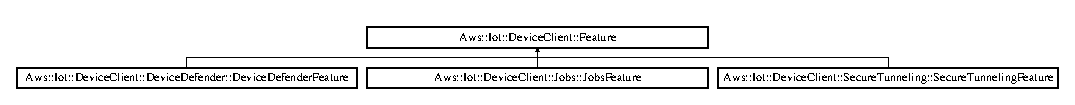
\includegraphics[height=0.959726cm]{class_aws_1_1_iot_1_1_device_client_1_1_feature}
\end{center}
\end{figure}
\subsection*{Public Member Functions}
\begin{DoxyCompactItemize}
\item 
virtual int \hyperlink{class_aws_1_1_iot_1_1_device_client_1_1_feature_ac9a936ebd88f7e35914a6aac99badf7d}{start} ()=0
\begin{DoxyCompactList}\small\item\em Start the feature. \end{DoxyCompactList}\item 
virtual int \hyperlink{class_aws_1_1_iot_1_1_device_client_1_1_feature_a5b672f7b1403512cad9104ba923fc73d}{stop} ()=0
\begin{DoxyCompactList}\small\item\em Stop the feature. \end{DoxyCompactList}\item 
virtual std\+::string \hyperlink{class_aws_1_1_iot_1_1_device_client_1_1_feature_a7f56b81457898d67ddc1942e57e3c0d5}{get\+Name} ()=0
\begin{DoxyCompactList}\small\item\em For a given feature, returns its name. \end{DoxyCompactList}\end{DoxyCompactItemize}


\subsection{Detailed Description}
Common interface for orchestration of Device Client features. 

The \hyperlink{class_aws_1_1_iot_1_1_device_client_1_1_feature}{Feature} interface provides some basic methods for orchestrating the individual features running as part of the Device Client (DC). The \hyperlink{class_aws_1_1_iot_1_1_device_client_1_1_feature_ac9a936ebd88f7e35914a6aac99badf7d}{start()} and \hyperlink{class_aws_1_1_iot_1_1_device_client_1_1_feature_a5b672f7b1403512cad9104ba923fc73d}{stop()} methods allow the agent base (main.\+cpp) to either start operation of the feature after performing initialization or to stop a feature in the event that it receives a signal indicating that the program must shut down as soon as possible. 

\subsection{Member Function Documentation}
\mbox{\Hypertarget{class_aws_1_1_iot_1_1_device_client_1_1_feature_a7f56b81457898d67ddc1942e57e3c0d5}\label{class_aws_1_1_iot_1_1_device_client_1_1_feature_a7f56b81457898d67ddc1942e57e3c0d5}} 
\index{Aws\+::\+Iot\+::\+Device\+Client\+::\+Feature@{Aws\+::\+Iot\+::\+Device\+Client\+::\+Feature}!get\+Name@{get\+Name}}
\index{get\+Name@{get\+Name}!Aws\+::\+Iot\+::\+Device\+Client\+::\+Feature@{Aws\+::\+Iot\+::\+Device\+Client\+::\+Feature}}
\subsubsection{\texorpdfstring{get\+Name()}{getName()}}
{\footnotesize\ttfamily virtual std\+::string Aws\+::\+Iot\+::\+Device\+Client\+::\+Feature\+::get\+Name (\begin{DoxyParamCaption}{ }\end{DoxyParamCaption})\hspace{0.3cm}{\ttfamily [pure virtual]}}



For a given feature, returns its name. 

\begin{DoxyReturn}{Returns}
a string value representing the feature\textquotesingle{}s name 
\end{DoxyReturn}


Implemented in \hyperlink{class_aws_1_1_iot_1_1_device_client_1_1_jobs_1_1_jobs_feature_a88bff915e713b132ce5a49a3d60ba294}{Aws\+::\+Iot\+::\+Device\+Client\+::\+Jobs\+::\+Jobs\+Feature}, \hyperlink{class_aws_1_1_iot_1_1_device_client_1_1_secure_tunneling_1_1_secure_tunneling_feature_accc93db855be85847c3472754439594f}{Aws\+::\+Iot\+::\+Device\+Client\+::\+Secure\+Tunneling\+::\+Secure\+Tunneling\+Feature}, and \hyperlink{class_aws_1_1_iot_1_1_device_client_1_1_device_defender_1_1_device_defender_feature_a5d1c425fb35d74caff528e7b59026211}{Aws\+::\+Iot\+::\+Device\+Client\+::\+Device\+Defender\+::\+Device\+Defender\+Feature}.

\mbox{\Hypertarget{class_aws_1_1_iot_1_1_device_client_1_1_feature_ac9a936ebd88f7e35914a6aac99badf7d}\label{class_aws_1_1_iot_1_1_device_client_1_1_feature_ac9a936ebd88f7e35914a6aac99badf7d}} 
\index{Aws\+::\+Iot\+::\+Device\+Client\+::\+Feature@{Aws\+::\+Iot\+::\+Device\+Client\+::\+Feature}!start@{start}}
\index{start@{start}!Aws\+::\+Iot\+::\+Device\+Client\+::\+Feature@{Aws\+::\+Iot\+::\+Device\+Client\+::\+Feature}}
\subsubsection{\texorpdfstring{start()}{start()}}
{\footnotesize\ttfamily virtual int Aws\+::\+Iot\+::\+Device\+Client\+::\+Feature\+::start (\begin{DoxyParamCaption}{ }\end{DoxyParamCaption})\hspace{0.3cm}{\ttfamily [pure virtual]}}



Start the feature. 

\begin{DoxyReturn}{Returns}
an integer representing the S\+U\+C\+C\+E\+SS or F\+A\+I\+L\+U\+RE of the \hyperlink{class_aws_1_1_iot_1_1_device_client_1_1_feature_ac9a936ebd88f7e35914a6aac99badf7d}{start()} operation on the feature 
\end{DoxyReturn}


Implemented in \hyperlink{class_aws_1_1_iot_1_1_device_client_1_1_jobs_1_1_jobs_feature_a6369b1914ce964ca98c9474a38e3214f}{Aws\+::\+Iot\+::\+Device\+Client\+::\+Jobs\+::\+Jobs\+Feature}, \hyperlink{class_aws_1_1_iot_1_1_device_client_1_1_secure_tunneling_1_1_secure_tunneling_feature_a9e33fc786883e519e587f7d89f2a9086}{Aws\+::\+Iot\+::\+Device\+Client\+::\+Secure\+Tunneling\+::\+Secure\+Tunneling\+Feature}, and \hyperlink{class_aws_1_1_iot_1_1_device_client_1_1_device_defender_1_1_device_defender_feature_aeede868840f237a50d394c779a8a9026}{Aws\+::\+Iot\+::\+Device\+Client\+::\+Device\+Defender\+::\+Device\+Defender\+Feature}.

\mbox{\Hypertarget{class_aws_1_1_iot_1_1_device_client_1_1_feature_a5b672f7b1403512cad9104ba923fc73d}\label{class_aws_1_1_iot_1_1_device_client_1_1_feature_a5b672f7b1403512cad9104ba923fc73d}} 
\index{Aws\+::\+Iot\+::\+Device\+Client\+::\+Feature@{Aws\+::\+Iot\+::\+Device\+Client\+::\+Feature}!stop@{stop}}
\index{stop@{stop}!Aws\+::\+Iot\+::\+Device\+Client\+::\+Feature@{Aws\+::\+Iot\+::\+Device\+Client\+::\+Feature}}
\subsubsection{\texorpdfstring{stop()}{stop()}}
{\footnotesize\ttfamily virtual int Aws\+::\+Iot\+::\+Device\+Client\+::\+Feature\+::stop (\begin{DoxyParamCaption}{ }\end{DoxyParamCaption})\hspace{0.3cm}{\ttfamily [pure virtual]}}



Stop the feature. 

\begin{DoxyReturn}{Returns}
an integer representing the S\+U\+C\+C\+E\+SS or F\+A\+I\+L\+U\+RE of the \hyperlink{class_aws_1_1_iot_1_1_device_client_1_1_feature_a5b672f7b1403512cad9104ba923fc73d}{stop()} operation on the feature 
\end{DoxyReturn}


Implemented in \hyperlink{class_aws_1_1_iot_1_1_device_client_1_1_jobs_1_1_jobs_feature_aeec6332d60872b2a4471f6494f93b1c4}{Aws\+::\+Iot\+::\+Device\+Client\+::\+Jobs\+::\+Jobs\+Feature}, \hyperlink{class_aws_1_1_iot_1_1_device_client_1_1_secure_tunneling_1_1_secure_tunneling_feature_a9cd3840b50bd1f62537df3354c7d2fbf}{Aws\+::\+Iot\+::\+Device\+Client\+::\+Secure\+Tunneling\+::\+Secure\+Tunneling\+Feature}, and \hyperlink{class_aws_1_1_iot_1_1_device_client_1_1_device_defender_1_1_device_defender_feature_a93b78c0fe8518baabdff3d38544b9d00}{Aws\+::\+Iot\+::\+Device\+Client\+::\+Device\+Defender\+::\+Device\+Defender\+Feature}.



The documentation for this class was generated from the following file\+:\begin{DoxyCompactItemize}
\item 
/home/\+A\+N\+T.\+A\+M\+A\+Z\+O\+N.\+C\+O\+M/lwwilkov/\+Workspace/aws-\/iot-\/device-\/client/source/Feature.\+h\end{DoxyCompactItemize}

\hypertarget{class_aws_1_1_iot_1_1_device_client_1_1_logging_1_1_file_logger}{}\doxysection{Aws\+::Iot\+::Device\+Client\+::Logging\+::File\+Logger Class Reference}
\label{class_aws_1_1_iot_1_1_device_client_1_1_logging_1_1_file_logger}\index{Aws::Iot::DeviceClient::Logging::FileLogger@{Aws::Iot::DeviceClient::Logging::FileLogger}}


File-\/based logging implementation for writing log messages to a file on the device.  




{\ttfamily \#include $<$File\+Logger.\+h$>$}

Inheritance diagram for Aws\+::Iot\+::Device\+Client\+::Logging\+::File\+Logger\+:\begin{figure}[H]
\begin{center}
\leavevmode
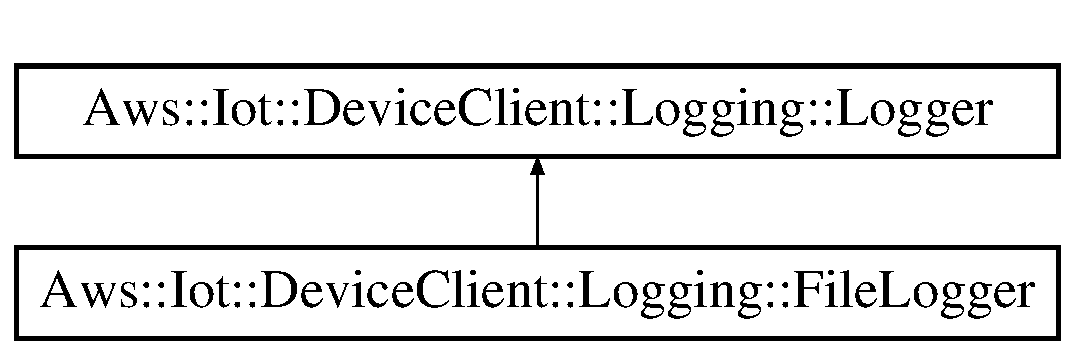
\includegraphics[height=2.000000cm]{class_aws_1_1_iot_1_1_device_client_1_1_logging_1_1_file_logger}
\end{center}
\end{figure}
\doxysubsection*{Public Member Functions}
\begin{DoxyCompactItemize}
\item 
virtual bool \mbox{\hyperlink{class_aws_1_1_iot_1_1_device_client_1_1_logging_1_1_file_logger_ac9373269d6d5c7a5ee1ba896182c97ff}{start}} (const \mbox{\hyperlink{struct_aws_1_1_iot_1_1_device_client_1_1_plain_config}{Plain\+Config}} \&config) override
\begin{DoxyCompactList}\small\item\em Starts the underlying logger implementation\textquotesingle{}s logging behavior. \end{DoxyCompactList}\item 
\mbox{\Hypertarget{class_aws_1_1_iot_1_1_device_client_1_1_logging_1_1_file_logger_a31cbe6ad19051138966eae72ff233702}\label{class_aws_1_1_iot_1_1_device_client_1_1_logging_1_1_file_logger_a31cbe6ad19051138966eae72ff233702}} 
virtual void \mbox{\hyperlink{class_aws_1_1_iot_1_1_device_client_1_1_logging_1_1_file_logger_a31cbe6ad19051138966eae72ff233702}{stop}} () override
\begin{DoxyCompactList}\small\item\em Attempts to stop the \mbox{\hyperlink{class_aws_1_1_iot_1_1_device_client_1_1_logging_1_1_logger}{Logger}} implementation from writing any additional log messages, likely to switch to a different logger implementation. \end{DoxyCompactList}\item 
\mbox{\Hypertarget{class_aws_1_1_iot_1_1_device_client_1_1_logging_1_1_file_logger_a7cbd7f8942bc9da32a9ff385128d5519}\label{class_aws_1_1_iot_1_1_device_client_1_1_logging_1_1_file_logger_a7cbd7f8942bc9da32a9ff385128d5519}} 
virtual void \mbox{\hyperlink{class_aws_1_1_iot_1_1_device_client_1_1_logging_1_1_file_logger_a7cbd7f8942bc9da32a9ff385128d5519}{shutdown}} () override
\begin{DoxyCompactList}\small\item\em Notifies the \mbox{\hyperlink{class_aws_1_1_iot_1_1_device_client_1_1_logging_1_1_logger}{Logger}} implementation that any queued logs should be dumped to output and the logger should shut itself down. \end{DoxyCompactList}\item 
virtual std\+::unique\+\_\+ptr$<$ \mbox{\hyperlink{class_aws_1_1_iot_1_1_device_client_1_1_logging_1_1_log_queue}{Log\+Queue}} $>$ \mbox{\hyperlink{class_aws_1_1_iot_1_1_device_client_1_1_logging_1_1_file_logger_a5c55467d8f46332d6ef2acde379df2f7}{take\+Log\+Queue}} () override
\begin{DoxyCompactList}\small\item\em Removes the \mbox{\hyperlink{class_aws_1_1_iot_1_1_device_client_1_1_logging_1_1_log_queue}{Log\+Queue}} from the logger implementation so it can be passed to another logger implementation for processing. \end{DoxyCompactList}\item 
virtual void \mbox{\hyperlink{class_aws_1_1_iot_1_1_device_client_1_1_logging_1_1_file_logger_a42b047d2f2379638add126414690d65d}{set\+Log\+Queue}} (std\+::unique\+\_\+ptr$<$ \mbox{\hyperlink{class_aws_1_1_iot_1_1_device_client_1_1_logging_1_1_log_queue}{Log\+Queue}} $>$ \mbox{\hyperlink{class_aws_1_1_iot_1_1_device_client_1_1_logging_1_1_file_logger_a9d9cf4cb8c016d0f364bbf182e41c1fe}{log\+Queue}}) override
\begin{DoxyCompactList}\small\item\em Passes a \mbox{\hyperlink{class_aws_1_1_iot_1_1_device_client_1_1_logging_1_1_log_queue}{Log\+Queue}} to the logger implementation. Typically used if the logger implementation is being changed. \end{DoxyCompactList}\item 
virtual void \mbox{\hyperlink{class_aws_1_1_iot_1_1_device_client_1_1_logging_1_1_file_logger_a507513cb4aca226a5ed6da292bfd915a}{flush}} () override
\begin{DoxyCompactList}\small\item\em Flush the log output from the queue synchronously. \end{DoxyCompactList}\end{DoxyCompactItemize}
\doxysubsection*{Private Member Functions}
\begin{DoxyCompactItemize}
\item 
void \mbox{\hyperlink{class_aws_1_1_iot_1_1_device_client_1_1_logging_1_1_file_logger_aea84d831a8e014a164b85504dd755466}{write\+Log\+Message}} (std\+::unique\+\_\+ptr$<$ \mbox{\hyperlink{class_aws_1_1_iot_1_1_device_client_1_1_logging_1_1_log_message}{Log\+Message}} $>$ message)
\begin{DoxyCompactList}\small\item\em Write the log message to the log file. \end{DoxyCompactList}\item 
void \mbox{\hyperlink{class_aws_1_1_iot_1_1_device_client_1_1_logging_1_1_file_logger_adb5a5536099975ee80b04b1635112d52}{create\+Log\+Directories}} ()
\begin{DoxyCompactList}\small\item\em Creates the directories required as part of the full path to the desired log file. \end{DoxyCompactList}\item 
void \mbox{\hyperlink{class_aws_1_1_iot_1_1_device_client_1_1_logging_1_1_file_logger_a3c6b08640df02c4065c358523dc6a37d}{run}} ()
\begin{DoxyCompactList}\small\item\em Begins processing of log messages in the \mbox{\hyperlink{class_aws_1_1_iot_1_1_device_client_1_1_logging_1_1_log_queue}{Log\+Queue}}. \end{DoxyCompactList}\item 
virtual void \mbox{\hyperlink{class_aws_1_1_iot_1_1_device_client_1_1_logging_1_1_file_logger_a549cf9783ce070e514c0f68340ae5d1c}{queue\+Log}} (Log\+Level level, const char $\ast$tag, std\+::chrono\+::time\+\_\+point$<$ std\+::chrono\+::system\+\_\+clock $>$ t, std\+::string message) override
\begin{DoxyCompactList}\small\item\em Implemented by the underlying logger implementation to pass responsibility for managing the log message from the \mbox{\hyperlink{class_aws_1_1_iot_1_1_device_client_1_1_logging_1_1_logger}{Logger}} interface to the logger implementation. \end{DoxyCompactList}\end{DoxyCompactItemize}
\doxysubsection*{Private Attributes}
\begin{DoxyCompactItemize}
\item 
std\+::string \mbox{\hyperlink{class_aws_1_1_iot_1_1_device_client_1_1_logging_1_1_file_logger_a771b31b2f05b4f8fa29de755f15eb35c}{D\+E\+F\+A\+U\+L\+T\+\_\+\+L\+O\+G\+\_\+\+F\+I\+LE}} = \char`\"{}/var/log/aws-\/iot-\/device-\/client/aws-\/iot-\/device-\/client.\+log\char`\"{}
\begin{DoxyCompactList}\small\item\em The full path to the default log file for the Device Client. \end{DoxyCompactList}\item 
\mbox{\Hypertarget{class_aws_1_1_iot_1_1_device_client_1_1_logging_1_1_file_logger_abb78588623916c835dbca8751995f8cd}\label{class_aws_1_1_iot_1_1_device_client_1_1_logging_1_1_file_logger_abb78588623916c835dbca8751995f8cd}} 
std\+::string \mbox{\hyperlink{class_aws_1_1_iot_1_1_device_client_1_1_logging_1_1_file_logger_abb78588623916c835dbca8751995f8cd}{log\+File}} = \mbox{\hyperlink{class_aws_1_1_iot_1_1_device_client_1_1_logging_1_1_file_logger_a771b31b2f05b4f8fa29de755f15eb35c}{D\+E\+F\+A\+U\+L\+T\+\_\+\+L\+O\+G\+\_\+\+F\+I\+LE}}
\begin{DoxyCompactList}\small\item\em Runtime configuration for which log file to log to. \end{DoxyCompactList}\item 
\mbox{\Hypertarget{class_aws_1_1_iot_1_1_device_client_1_1_logging_1_1_file_logger_a0e7a54d7e865f03ba082821248e4beef}\label{class_aws_1_1_iot_1_1_device_client_1_1_logging_1_1_file_logger_a0e7a54d7e865f03ba082821248e4beef}} 
bool \mbox{\hyperlink{class_aws_1_1_iot_1_1_device_client_1_1_logging_1_1_file_logger_a0e7a54d7e865f03ba082821248e4beef}{needs\+Shutdown}} = false
\begin{DoxyCompactList}\small\item\em Flag used to notify underlying threads that they should discontinue any processing so that the application can safely shutdown. \end{DoxyCompactList}\item 
\mbox{\Hypertarget{class_aws_1_1_iot_1_1_device_client_1_1_logging_1_1_file_logger_aae7badd8eb227b7207210e817c111188}\label{class_aws_1_1_iot_1_1_device_client_1_1_logging_1_1_file_logger_aae7badd8eb227b7207210e817c111188}} 
std\+::mutex {\bfseries is\+Running\+Lock}
\item 
\mbox{\Hypertarget{class_aws_1_1_iot_1_1_device_client_1_1_logging_1_1_file_logger_a7c85906ad319df437506fa462dc7947a}\label{class_aws_1_1_iot_1_1_device_client_1_1_logging_1_1_file_logger_a7c85906ad319df437506fa462dc7947a}} 
bool {\bfseries is\+Running} = false
\item 
\mbox{\Hypertarget{class_aws_1_1_iot_1_1_device_client_1_1_logging_1_1_file_logger_a9d9cf4cb8c016d0f364bbf182e41c1fe}\label{class_aws_1_1_iot_1_1_device_client_1_1_logging_1_1_file_logger_a9d9cf4cb8c016d0f364bbf182e41c1fe}} 
std\+::unique\+\_\+ptr$<$ \mbox{\hyperlink{class_aws_1_1_iot_1_1_device_client_1_1_logging_1_1_log_queue}{Log\+Queue}} $>$ \mbox{\hyperlink{class_aws_1_1_iot_1_1_device_client_1_1_logging_1_1_file_logger_a9d9cf4cb8c016d0f364bbf182e41c1fe}{log\+Queue}} = std\+::unique\+\_\+ptr$<$\mbox{\hyperlink{class_aws_1_1_iot_1_1_device_client_1_1_logging_1_1_log_queue}{Log\+Queue}}$>$(new \mbox{\hyperlink{class_aws_1_1_iot_1_1_device_client_1_1_logging_1_1_log_queue}{Log\+Queue}})
\begin{DoxyCompactList}\small\item\em a \mbox{\hyperlink{class_aws_1_1_iot_1_1_device_client_1_1_logging_1_1_log_queue}{Log\+Queue}} instance used to queue incoming log messages for processing \end{DoxyCompactList}\item 
\mbox{\Hypertarget{class_aws_1_1_iot_1_1_device_client_1_1_logging_1_1_file_logger_a32c72325d8fdf1aa7b65911c50f6be30}\label{class_aws_1_1_iot_1_1_device_client_1_1_logging_1_1_file_logger_a32c72325d8fdf1aa7b65911c50f6be30}} 
std\+::unique\+\_\+ptr$<$ std\+::ofstream $>$ \mbox{\hyperlink{class_aws_1_1_iot_1_1_device_client_1_1_logging_1_1_file_logger_a32c72325d8fdf1aa7b65911c50f6be30}{output\+Stream}}
\begin{DoxyCompactList}\small\item\em an std\+::ofstream representing an underlying file that is used to write log output to disk \end{DoxyCompactList}\end{DoxyCompactItemize}
\doxysubsection*{Additional Inherited Members}


\doxysubsection{Detailed Description}
File-\/based logging implementation for writing log messages to a file on the device. 

\doxysubsection{Member Function Documentation}
\mbox{\Hypertarget{class_aws_1_1_iot_1_1_device_client_1_1_logging_1_1_file_logger_adb5a5536099975ee80b04b1635112d52}\label{class_aws_1_1_iot_1_1_device_client_1_1_logging_1_1_file_logger_adb5a5536099975ee80b04b1635112d52}} 
\index{Aws::Iot::DeviceClient::Logging::FileLogger@{Aws::Iot::DeviceClient::Logging::FileLogger}!createLogDirectories@{createLogDirectories}}
\index{createLogDirectories@{createLogDirectories}!Aws::Iot::DeviceClient::Logging::FileLogger@{Aws::Iot::DeviceClient::Logging::FileLogger}}
\doxysubsubsection{\texorpdfstring{createLogDirectories()}{createLogDirectories()}}
{\footnotesize\ttfamily void Aws\+::\+Iot\+::\+Device\+Client\+::\+Logging\+::\+File\+Logger\+::create\+Log\+Directories (\begin{DoxyParamCaption}{ }\end{DoxyParamCaption})\hspace{0.3cm}{\ttfamily [private]}}



Creates the directories required as part of the full path to the desired log file. 

This method is run as part of the initialization process of the \mbox{\hyperlink{class_aws_1_1_iot_1_1_device_client_1_1_logging_1_1_file_logger}{File\+Logger}} implementation to create any directories required as part of the full path to the desired log file \mbox{\Hypertarget{class_aws_1_1_iot_1_1_device_client_1_1_logging_1_1_file_logger_a507513cb4aca226a5ed6da292bfd915a}\label{class_aws_1_1_iot_1_1_device_client_1_1_logging_1_1_file_logger_a507513cb4aca226a5ed6da292bfd915a}} 
\index{Aws::Iot::DeviceClient::Logging::FileLogger@{Aws::Iot::DeviceClient::Logging::FileLogger}!flush@{flush}}
\index{flush@{flush}!Aws::Iot::DeviceClient::Logging::FileLogger@{Aws::Iot::DeviceClient::Logging::FileLogger}}
\doxysubsubsection{\texorpdfstring{flush()}{flush()}}
{\footnotesize\ttfamily void File\+Logger\+::flush (\begin{DoxyParamCaption}{ }\end{DoxyParamCaption})\hspace{0.3cm}{\ttfamily [override]}, {\ttfamily [virtual]}}



Flush the log output from the queue synchronously. 

This is helpful for scenarios where you need to ensure that the logs are written to disk before any other activity takes place. Note that this will not block other threads, only the thread that this is called from 

Implements \mbox{\hyperlink{class_aws_1_1_iot_1_1_device_client_1_1_logging_1_1_logger_a4743383e9c69bec10ba970dc4394781e}{Aws\+::\+Iot\+::\+Device\+Client\+::\+Logging\+::\+Logger}}.

\mbox{\Hypertarget{class_aws_1_1_iot_1_1_device_client_1_1_logging_1_1_file_logger_a549cf9783ce070e514c0f68340ae5d1c}\label{class_aws_1_1_iot_1_1_device_client_1_1_logging_1_1_file_logger_a549cf9783ce070e514c0f68340ae5d1c}} 
\index{Aws::Iot::DeviceClient::Logging::FileLogger@{Aws::Iot::DeviceClient::Logging::FileLogger}!queueLog@{queueLog}}
\index{queueLog@{queueLog}!Aws::Iot::DeviceClient::Logging::FileLogger@{Aws::Iot::DeviceClient::Logging::FileLogger}}
\doxysubsubsection{\texorpdfstring{queueLog()}{queueLog()}}
{\footnotesize\ttfamily void File\+Logger\+::queue\+Log (\begin{DoxyParamCaption}\item[{Log\+Level}]{level,  }\item[{const char $\ast$}]{tag,  }\item[{std\+::chrono\+::time\+\_\+point$<$ std\+::chrono\+::system\+\_\+clock $>$}]{t,  }\item[{std\+::string}]{message }\end{DoxyParamCaption})\hspace{0.3cm}{\ttfamily [override]}, {\ttfamily [private]}, {\ttfamily [virtual]}}



Implemented by the underlying logger implementation to pass responsibility for managing the log message from the \mbox{\hyperlink{class_aws_1_1_iot_1_1_device_client_1_1_logging_1_1_logger}{Logger}} interface to the logger implementation. 

This virtual method should be implemented by the underlying logger implementation to actually accept and eventually process the incoming log message. To reduce complications induced by multithreading, the underlying logger implementation should queue the message for processing by another thread if possible. 
\begin{DoxyParams}{Parameters}
{\em level} & the log level \\
\hline
{\em tag} & a tag that indicates where the log message is coming from \\
\hline
{\em t} & a timestamp representing the time the message was created \\
\hline
{\em message} & the message to log \\
\hline
\end{DoxyParams}


Implements \mbox{\hyperlink{class_aws_1_1_iot_1_1_device_client_1_1_logging_1_1_logger_a75acdae576e13ddd84bccb70d8fb1fef}{Aws\+::\+Iot\+::\+Device\+Client\+::\+Logging\+::\+Logger}}.

\mbox{\Hypertarget{class_aws_1_1_iot_1_1_device_client_1_1_logging_1_1_file_logger_a3c6b08640df02c4065c358523dc6a37d}\label{class_aws_1_1_iot_1_1_device_client_1_1_logging_1_1_file_logger_a3c6b08640df02c4065c358523dc6a37d}} 
\index{Aws::Iot::DeviceClient::Logging::FileLogger@{Aws::Iot::DeviceClient::Logging::FileLogger}!run@{run}}
\index{run@{run}!Aws::Iot::DeviceClient::Logging::FileLogger@{Aws::Iot::DeviceClient::Logging::FileLogger}}
\doxysubsubsection{\texorpdfstring{run()}{run()}}
{\footnotesize\ttfamily void File\+Logger\+::run (\begin{DoxyParamCaption}{ }\end{DoxyParamCaption})\hspace{0.3cm}{\ttfamily [private]}}



Begins processing of log messages in the \mbox{\hyperlink{class_aws_1_1_iot_1_1_device_client_1_1_logging_1_1_log_queue}{Log\+Queue}}. 

This method will begin processing of log messages in the \mbox{\hyperlink{class_aws_1_1_iot_1_1_device_client_1_1_logging_1_1_log_queue}{Log\+Queue}}. The thread will process until all of the messages are removed from the queue, and then will wait until new messages arrive in the queue. This method will check to make sure the \mbox{\hyperlink{class_aws_1_1_iot_1_1_device_client_1_1_logging_1_1_file_logger_a7cbd7f8942bc9da32a9ff385128d5519}{shutdown()}} method has not been called before processing any additional messages in the queue. \mbox{\Hypertarget{class_aws_1_1_iot_1_1_device_client_1_1_logging_1_1_file_logger_a42b047d2f2379638add126414690d65d}\label{class_aws_1_1_iot_1_1_device_client_1_1_logging_1_1_file_logger_a42b047d2f2379638add126414690d65d}} 
\index{Aws::Iot::DeviceClient::Logging::FileLogger@{Aws::Iot::DeviceClient::Logging::FileLogger}!setLogQueue@{setLogQueue}}
\index{setLogQueue@{setLogQueue}!Aws::Iot::DeviceClient::Logging::FileLogger@{Aws::Iot::DeviceClient::Logging::FileLogger}}
\doxysubsubsection{\texorpdfstring{setLogQueue()}{setLogQueue()}}
{\footnotesize\ttfamily void File\+Logger\+::set\+Log\+Queue (\begin{DoxyParamCaption}\item[{std\+::unique\+\_\+ptr$<$ \mbox{\hyperlink{class_aws_1_1_iot_1_1_device_client_1_1_logging_1_1_log_queue}{Log\+Queue}} $>$}]{log\+Queue }\end{DoxyParamCaption})\hspace{0.3cm}{\ttfamily [override]}, {\ttfamily [virtual]}}



Passes a \mbox{\hyperlink{class_aws_1_1_iot_1_1_device_client_1_1_logging_1_1_log_queue}{Log\+Queue}} to the logger implementation. Typically used if the logger implementation is being changed. 


\begin{DoxyParams}{Parameters}
{\em log\+Queue} & \\
\hline
\end{DoxyParams}


Implements \mbox{\hyperlink{class_aws_1_1_iot_1_1_device_client_1_1_logging_1_1_logger_a6b80ca4200fbc58bb2994ef4319ea822}{Aws\+::\+Iot\+::\+Device\+Client\+::\+Logging\+::\+Logger}}.

\mbox{\Hypertarget{class_aws_1_1_iot_1_1_device_client_1_1_logging_1_1_file_logger_ac9373269d6d5c7a5ee1ba896182c97ff}\label{class_aws_1_1_iot_1_1_device_client_1_1_logging_1_1_file_logger_ac9373269d6d5c7a5ee1ba896182c97ff}} 
\index{Aws::Iot::DeviceClient::Logging::FileLogger@{Aws::Iot::DeviceClient::Logging::FileLogger}!start@{start}}
\index{start@{start}!Aws::Iot::DeviceClient::Logging::FileLogger@{Aws::Iot::DeviceClient::Logging::FileLogger}}
\doxysubsubsection{\texorpdfstring{start()}{start()}}
{\footnotesize\ttfamily bool File\+Logger\+::start (\begin{DoxyParamCaption}\item[{const \mbox{\hyperlink{struct_aws_1_1_iot_1_1_device_client_1_1_plain_config}{Plain\+Config}} \&}]{config }\end{DoxyParamCaption})\hspace{0.3cm}{\ttfamily [override]}, {\ttfamily [virtual]}}



Starts the underlying logger implementation\textquotesingle{}s logging behavior. 


\begin{DoxyParams}{Parameters}
{\em config} & the config data passed in from the C\+LI and J\+S\+ON \\
\hline
\end{DoxyParams}
\begin{DoxyReturn}{Returns}
true if it is able to start successfully, false otherwise 
\end{DoxyReturn}


Implements \mbox{\hyperlink{class_aws_1_1_iot_1_1_device_client_1_1_logging_1_1_logger_ad42e38afcd7402f5dc1213b2f0b96961}{Aws\+::\+Iot\+::\+Device\+Client\+::\+Logging\+::\+Logger}}.

\mbox{\Hypertarget{class_aws_1_1_iot_1_1_device_client_1_1_logging_1_1_file_logger_a5c55467d8f46332d6ef2acde379df2f7}\label{class_aws_1_1_iot_1_1_device_client_1_1_logging_1_1_file_logger_a5c55467d8f46332d6ef2acde379df2f7}} 
\index{Aws::Iot::DeviceClient::Logging::FileLogger@{Aws::Iot::DeviceClient::Logging::FileLogger}!takeLogQueue@{takeLogQueue}}
\index{takeLogQueue@{takeLogQueue}!Aws::Iot::DeviceClient::Logging::FileLogger@{Aws::Iot::DeviceClient::Logging::FileLogger}}
\doxysubsubsection{\texorpdfstring{takeLogQueue()}{takeLogQueue()}}
{\footnotesize\ttfamily unique\+\_\+ptr$<$ \mbox{\hyperlink{class_aws_1_1_iot_1_1_device_client_1_1_logging_1_1_log_queue}{Log\+Queue}} $>$ File\+Logger\+::take\+Log\+Queue (\begin{DoxyParamCaption}{ }\end{DoxyParamCaption})\hspace{0.3cm}{\ttfamily [override]}, {\ttfamily [virtual]}}



Removes the \mbox{\hyperlink{class_aws_1_1_iot_1_1_device_client_1_1_logging_1_1_log_queue}{Log\+Queue}} from the logger implementation so it can be passed to another logger implementation for processing. 

\begin{DoxyReturn}{Returns}
a unique\+\_\+ptr$<$\+Log\+Queue$>$ 
\end{DoxyReturn}


Implements \mbox{\hyperlink{class_aws_1_1_iot_1_1_device_client_1_1_logging_1_1_logger_a39f3326be17f9ed4b1385f057134774d}{Aws\+::\+Iot\+::\+Device\+Client\+::\+Logging\+::\+Logger}}.

\mbox{\Hypertarget{class_aws_1_1_iot_1_1_device_client_1_1_logging_1_1_file_logger_aea84d831a8e014a164b85504dd755466}\label{class_aws_1_1_iot_1_1_device_client_1_1_logging_1_1_file_logger_aea84d831a8e014a164b85504dd755466}} 
\index{Aws::Iot::DeviceClient::Logging::FileLogger@{Aws::Iot::DeviceClient::Logging::FileLogger}!writeLogMessage@{writeLogMessage}}
\index{writeLogMessage@{writeLogMessage}!Aws::Iot::DeviceClient::Logging::FileLogger@{Aws::Iot::DeviceClient::Logging::FileLogger}}
\doxysubsubsection{\texorpdfstring{writeLogMessage()}{writeLogMessage()}}
{\footnotesize\ttfamily void File\+Logger\+::write\+Log\+Message (\begin{DoxyParamCaption}\item[{std\+::unique\+\_\+ptr$<$ \mbox{\hyperlink{class_aws_1_1_iot_1_1_device_client_1_1_logging_1_1_log_message}{Log\+Message}} $>$}]{message }\end{DoxyParamCaption})\hspace{0.3cm}{\ttfamily [private]}}



Write the log message to the log file. 

This method will write the log message to the file specified for logging 
\begin{DoxyParams}{Parameters}
{\em message} & the message to log \\
\hline
\end{DoxyParams}


\doxysubsection{Member Data Documentation}
\mbox{\Hypertarget{class_aws_1_1_iot_1_1_device_client_1_1_logging_1_1_file_logger_a771b31b2f05b4f8fa29de755f15eb35c}\label{class_aws_1_1_iot_1_1_device_client_1_1_logging_1_1_file_logger_a771b31b2f05b4f8fa29de755f15eb35c}} 
\index{Aws::Iot::DeviceClient::Logging::FileLogger@{Aws::Iot::DeviceClient::Logging::FileLogger}!DEFAULT\_LOG\_FILE@{DEFAULT\_LOG\_FILE}}
\index{DEFAULT\_LOG\_FILE@{DEFAULT\_LOG\_FILE}!Aws::Iot::DeviceClient::Logging::FileLogger@{Aws::Iot::DeviceClient::Logging::FileLogger}}
\doxysubsubsection{\texorpdfstring{DEFAULT\_LOG\_FILE}{DEFAULT\_LOG\_FILE}}
{\footnotesize\ttfamily std\+::string Aws\+::\+Iot\+::\+Device\+Client\+::\+Logging\+::\+File\+Logger\+::\+D\+E\+F\+A\+U\+L\+T\+\_\+\+L\+O\+G\+\_\+\+F\+I\+LE = \char`\"{}/var/log/aws-\/iot-\/device-\/client/aws-\/iot-\/device-\/client.\+log\char`\"{}\hspace{0.3cm}{\ttfamily [private]}}



The full path to the default log file for the Device Client. 

If the user does not specify a desired log location in either the command line arguments or the Json configuration file, this is the default log that will be used 

The documentation for this class was generated from the following files\+:\begin{DoxyCompactItemize}
\item 
/home/runner/work/aws-\/iot-\/device-\/client/aws-\/iot-\/device-\/client/source/logging/File\+Logger.\+h\item 
/home/runner/work/aws-\/iot-\/device-\/client/aws-\/iot-\/device-\/client/source/logging/File\+Logger.\+cpp\end{DoxyCompactItemize}

\hypertarget{class_aws_1_1_iot_1_1_device_client_1_1_util_1_1_file_utils}{}\doxysection{Aws\+::Iot\+::Device\+Client\+::Util\+::File\+Utils Class Reference}
\label{class_aws_1_1_iot_1_1_device_client_1_1_util_1_1_file_utils}\index{Aws::Iot::DeviceClient::Util::FileUtils@{Aws::Iot::DeviceClient::Util::FileUtils}}


Utility functions for operations related to files.  




{\ttfamily \#include $<$File\+Utils.\+h$>$}

\doxysubsection*{Static Public Member Functions}
\begin{DoxyCompactItemize}
\item 
static int \mbox{\hyperlink{class_aws_1_1_iot_1_1_device_client_1_1_util_1_1_file_utils_acec1cd53ec38fcb34606141443dec4fe}{Mkdirs}} (const std\+::string \&path)
\begin{DoxyCompactList}\small\item\em Creates each of the directories in the provided path if they do not exist. \end{DoxyCompactList}\item 
static std\+::string \mbox{\hyperlink{class_aws_1_1_iot_1_1_device_client_1_1_util_1_1_file_utils_a137435480bde485798fe38cb63ae6b0d}{Extract\+Parent\+Directory}} (const std\+::string \&file\+Path)
\begin{DoxyCompactList}\small\item\em Given a path to a file, attempts to extract the parent directory. \end{DoxyCompactList}\item 
static std\+::string \mbox{\hyperlink{class_aws_1_1_iot_1_1_device_client_1_1_util_1_1_file_utils_ae1e32f8a3f157e2753c5eba96e7e3cd4}{Extract\+Expanded\+Path}} (const std\+::string \&file\+Path)
\begin{DoxyCompactList}\small\item\em Given a path to a file, attempts to extract the absolute path. \end{DoxyCompactList}\item 
static bool \mbox{\hyperlink{class_aws_1_1_iot_1_1_device_client_1_1_util_1_1_file_utils_a61556e62cd69ac493b7515d454927818}{Store\+Value\+In\+File}} (std\+::string value, std\+::string file\+Path)
\begin{DoxyCompactList}\small\item\em Stores string value in given file. \end{DoxyCompactList}\item 
static int \mbox{\hyperlink{class_aws_1_1_iot_1_1_device_client_1_1_util_1_1_file_utils_a19750e263a09c001b4d403ebcfee3472}{Get\+File\+Permissions}} (const std\+::string \&path)
\begin{DoxyCompactList}\small\item\em Returns an integer representing the permissions of the specified file. \end{DoxyCompactList}\item 
static bool \mbox{\hyperlink{class_aws_1_1_iot_1_1_device_client_1_1_util_1_1_file_utils_ab96cf791fb6c6093216c111d7d095ee9}{Validate\+File\+Ownership\+Permissions}} (const std\+::string \&path)
\begin{DoxyCompactList}\small\item\em Validates ownership permissions on the given file/dir. \end{DoxyCompactList}\item 
static bool \mbox{\hyperlink{class_aws_1_1_iot_1_1_device_client_1_1_util_1_1_file_utils_a9ea83b4248bea73525919cca6bb8c39d}{Validate\+File\+Permissions}} (const std\+::string \&path, const int file\+Permissions, bool fatal\+Error=true)
\begin{DoxyCompactList}\small\item\em Returns true if permissions set for given file/dir are correct. \end{DoxyCompactList}\item 
static int \mbox{\hyperlink{class_aws_1_1_iot_1_1_device_client_1_1_util_1_1_file_utils_af165bb643fa6c8aa0d6beace43275dcd}{Permissions\+Mask\+To\+Int}} (mode\+\_\+t mask)
\item 
static size\+\_\+t \mbox{\hyperlink{class_aws_1_1_iot_1_1_device_client_1_1_util_1_1_file_utils_a8f59952c80127b314abba046876830c0}{Get\+File\+Size}} (const std\+::string \&file\+Path)
\begin{DoxyCompactList}\small\item\em Returns the size of the file in bytes. \end{DoxyCompactList}\item 
static bool \mbox{\hyperlink{class_aws_1_1_iot_1_1_device_client_1_1_util_1_1_file_utils_a28fa5c453d546e54b07de465370b2b2e}{Create\+Directory\+With\+Permissions}} (const char $\ast$dir\+Path, mode\+\_\+t permissions)
\item 
static bool \mbox{\hyperlink{class_aws_1_1_iot_1_1_device_client_1_1_util_1_1_file_utils_af8008713194f85f0d601f41f1d59194d}{File\+Exists}} (const std\+::string \&filename)
\begin{DoxyCompactList}\small\item\em Check if the given filename exists. \end{DoxyCompactList}\end{DoxyCompactItemize}
\doxysubsection*{Static Private Attributes}
\begin{DoxyCompactItemize}
\item 
\mbox{\Hypertarget{class_aws_1_1_iot_1_1_device_client_1_1_util_1_1_file_utils_acea40b3e18d2999c94926e029eff0959}\label{class_aws_1_1_iot_1_1_device_client_1_1_util_1_1_file_utils_acea40b3e18d2999c94926e029eff0959}} 
static constexpr char {\bfseries T\+AG} \mbox{[}$\,$\mbox{]} = \char`\"{}File\+Utils.\+cpp\char`\"{}
\end{DoxyCompactItemize}


\doxysubsection{Detailed Description}
Utility functions for operations related to files. 

\doxysubsection{Member Function Documentation}
\mbox{\Hypertarget{class_aws_1_1_iot_1_1_device_client_1_1_util_1_1_file_utils_a28fa5c453d546e54b07de465370b2b2e}\label{class_aws_1_1_iot_1_1_device_client_1_1_util_1_1_file_utils_a28fa5c453d546e54b07de465370b2b2e}} 
\index{Aws::Iot::DeviceClient::Util::FileUtils@{Aws::Iot::DeviceClient::Util::FileUtils}!CreateDirectoryWithPermissions@{CreateDirectoryWithPermissions}}
\index{CreateDirectoryWithPermissions@{CreateDirectoryWithPermissions}!Aws::Iot::DeviceClient::Util::FileUtils@{Aws::Iot::DeviceClient::Util::FileUtils}}
\doxysubsubsection{\texorpdfstring{CreateDirectoryWithPermissions()}{CreateDirectoryWithPermissions()}}
{\footnotesize\ttfamily bool File\+Utils\+::\+Create\+Directory\+With\+Permissions (\begin{DoxyParamCaption}\item[{const char $\ast$}]{dir\+Path,  }\item[{mode\+\_\+t}]{permissions }\end{DoxyParamCaption})\hspace{0.3cm}{\ttfamily [static]}}

Attempts to create the provided directory with the given permissions 
\begin{DoxyParams}{Parameters}
{\em dir\+Path} & the path to the directory \\
\hline
{\em permissions} & the permission mask that should be applied to the directory \\
\hline
\end{DoxyParams}
\begin{DoxyReturn}{Returns}
true if the directory was successfully created with the given permissions, false otherwise 
\end{DoxyReturn}
\mbox{\Hypertarget{class_aws_1_1_iot_1_1_device_client_1_1_util_1_1_file_utils_ae1e32f8a3f157e2753c5eba96e7e3cd4}\label{class_aws_1_1_iot_1_1_device_client_1_1_util_1_1_file_utils_ae1e32f8a3f157e2753c5eba96e7e3cd4}} 
\index{Aws::Iot::DeviceClient::Util::FileUtils@{Aws::Iot::DeviceClient::Util::FileUtils}!ExtractExpandedPath@{ExtractExpandedPath}}
\index{ExtractExpandedPath@{ExtractExpandedPath}!Aws::Iot::DeviceClient::Util::FileUtils@{Aws::Iot::DeviceClient::Util::FileUtils}}
\doxysubsubsection{\texorpdfstring{ExtractExpandedPath()}{ExtractExpandedPath()}}
{\footnotesize\ttfamily string File\+Utils\+::\+Extract\+Expanded\+Path (\begin{DoxyParamCaption}\item[{const std\+::string \&}]{file\+Path }\end{DoxyParamCaption})\hspace{0.3cm}{\ttfamily [static]}}



Given a path to a file, attempts to extract the absolute path. 


\begin{DoxyParams}{Parameters}
{\em file\+Path} & a path to a file \\
\hline
\end{DoxyParams}
\begin{DoxyReturn}{Returns}
the expanded path of the file 
\end{DoxyReturn}
\mbox{\Hypertarget{class_aws_1_1_iot_1_1_device_client_1_1_util_1_1_file_utils_a137435480bde485798fe38cb63ae6b0d}\label{class_aws_1_1_iot_1_1_device_client_1_1_util_1_1_file_utils_a137435480bde485798fe38cb63ae6b0d}} 
\index{Aws::Iot::DeviceClient::Util::FileUtils@{Aws::Iot::DeviceClient::Util::FileUtils}!ExtractParentDirectory@{ExtractParentDirectory}}
\index{ExtractParentDirectory@{ExtractParentDirectory}!Aws::Iot::DeviceClient::Util::FileUtils@{Aws::Iot::DeviceClient::Util::FileUtils}}
\doxysubsubsection{\texorpdfstring{ExtractParentDirectory()}{ExtractParentDirectory()}}
{\footnotesize\ttfamily string File\+Utils\+::\+Extract\+Parent\+Directory (\begin{DoxyParamCaption}\item[{const std\+::string \&}]{file\+Path }\end{DoxyParamCaption})\hspace{0.3cm}{\ttfamily [static]}}



Given a path to a file, attempts to extract the parent directory. 


\begin{DoxyParams}{Parameters}
{\em file\+Path} & a path to a file \\
\hline
\end{DoxyParams}
\begin{DoxyReturn}{Returns}
the parent directory of the file 
\end{DoxyReturn}
\mbox{\Hypertarget{class_aws_1_1_iot_1_1_device_client_1_1_util_1_1_file_utils_af8008713194f85f0d601f41f1d59194d}\label{class_aws_1_1_iot_1_1_device_client_1_1_util_1_1_file_utils_af8008713194f85f0d601f41f1d59194d}} 
\index{Aws::Iot::DeviceClient::Util::FileUtils@{Aws::Iot::DeviceClient::Util::FileUtils}!FileExists@{FileExists}}
\index{FileExists@{FileExists}!Aws::Iot::DeviceClient::Util::FileUtils@{Aws::Iot::DeviceClient::Util::FileUtils}}
\doxysubsubsection{\texorpdfstring{FileExists()}{FileExists()}}
{\footnotesize\ttfamily bool File\+Utils\+::\+File\+Exists (\begin{DoxyParamCaption}\item[{const std\+::string \&}]{filename }\end{DoxyParamCaption})\hspace{0.3cm}{\ttfamily [static]}}



Check if the given filename exists. 


\begin{DoxyParams}{Parameters}
{\em filename} & Filename to check \\
\hline
\end{DoxyParams}
\begin{DoxyReturn}{Returns}
True if the file exists. False otherwise. 
\end{DoxyReturn}
\mbox{\Hypertarget{class_aws_1_1_iot_1_1_device_client_1_1_util_1_1_file_utils_a19750e263a09c001b4d403ebcfee3472}\label{class_aws_1_1_iot_1_1_device_client_1_1_util_1_1_file_utils_a19750e263a09c001b4d403ebcfee3472}} 
\index{Aws::Iot::DeviceClient::Util::FileUtils@{Aws::Iot::DeviceClient::Util::FileUtils}!GetFilePermissions@{GetFilePermissions}}
\index{GetFilePermissions@{GetFilePermissions}!Aws::Iot::DeviceClient::Util::FileUtils@{Aws::Iot::DeviceClient::Util::FileUtils}}
\doxysubsubsection{\texorpdfstring{GetFilePermissions()}{GetFilePermissions()}}
{\footnotesize\ttfamily int File\+Utils\+::\+Get\+File\+Permissions (\begin{DoxyParamCaption}\item[{const std\+::string \&}]{path }\end{DoxyParamCaption})\hspace{0.3cm}{\ttfamily [static]}}



Returns an integer representing the permissions of the specified file. 


\begin{DoxyParams}{Parameters}
{\em file\+Path} & a path to a file \\
\hline
\end{DoxyParams}
\begin{DoxyReturn}{Returns}
an integer representing the file permissions. 
\end{DoxyReturn}
\mbox{\Hypertarget{class_aws_1_1_iot_1_1_device_client_1_1_util_1_1_file_utils_a8f59952c80127b314abba046876830c0}\label{class_aws_1_1_iot_1_1_device_client_1_1_util_1_1_file_utils_a8f59952c80127b314abba046876830c0}} 
\index{Aws::Iot::DeviceClient::Util::FileUtils@{Aws::Iot::DeviceClient::Util::FileUtils}!GetFileSize@{GetFileSize}}
\index{GetFileSize@{GetFileSize}!Aws::Iot::DeviceClient::Util::FileUtils@{Aws::Iot::DeviceClient::Util::FileUtils}}
\doxysubsubsection{\texorpdfstring{GetFileSize()}{GetFileSize()}}
{\footnotesize\ttfamily size\+\_\+t File\+Utils\+::\+Get\+File\+Size (\begin{DoxyParamCaption}\item[{const std\+::string \&}]{file\+Path }\end{DoxyParamCaption})\hspace{0.3cm}{\ttfamily [static]}}



Returns the size of the file in bytes. 


\begin{DoxyParams}{Parameters}
{\em file\+Path} & the path to the file \\
\hline
\end{DoxyParams}
\begin{DoxyReturn}{Returns}
the size of the file in bytes 
\end{DoxyReturn}
\mbox{\Hypertarget{class_aws_1_1_iot_1_1_device_client_1_1_util_1_1_file_utils_acec1cd53ec38fcb34606141443dec4fe}\label{class_aws_1_1_iot_1_1_device_client_1_1_util_1_1_file_utils_acec1cd53ec38fcb34606141443dec4fe}} 
\index{Aws::Iot::DeviceClient::Util::FileUtils@{Aws::Iot::DeviceClient::Util::FileUtils}!Mkdirs@{Mkdirs}}
\index{Mkdirs@{Mkdirs}!Aws::Iot::DeviceClient::Util::FileUtils@{Aws::Iot::DeviceClient::Util::FileUtils}}
\doxysubsubsection{\texorpdfstring{Mkdirs()}{Mkdirs()}}
{\footnotesize\ttfamily int File\+Utils\+::\+Mkdirs (\begin{DoxyParamCaption}\item[{const std\+::string \&}]{path }\end{DoxyParamCaption})\hspace{0.3cm}{\ttfamily [static]}}



Creates each of the directories in the provided path if they do not exist. 


\begin{DoxyParams}{Parameters}
{\em path} & the full path to assess \\
\hline
\end{DoxyParams}
\begin{DoxyReturn}{Returns}
0 upon success, some other number indicating an error otherwise 
\end{DoxyReturn}
\mbox{\Hypertarget{class_aws_1_1_iot_1_1_device_client_1_1_util_1_1_file_utils_af165bb643fa6c8aa0d6beace43275dcd}\label{class_aws_1_1_iot_1_1_device_client_1_1_util_1_1_file_utils_af165bb643fa6c8aa0d6beace43275dcd}} 
\index{Aws::Iot::DeviceClient::Util::FileUtils@{Aws::Iot::DeviceClient::Util::FileUtils}!PermissionsMaskToInt@{PermissionsMaskToInt}}
\index{PermissionsMaskToInt@{PermissionsMaskToInt}!Aws::Iot::DeviceClient::Util::FileUtils@{Aws::Iot::DeviceClient::Util::FileUtils}}
\doxysubsubsection{\texorpdfstring{PermissionsMaskToInt()}{PermissionsMaskToInt()}}
{\footnotesize\ttfamily int File\+Utils\+::\+Permissions\+Mask\+To\+Int (\begin{DoxyParamCaption}\item[{mode\+\_\+t}]{mask }\end{DoxyParamCaption})\hspace{0.3cm}{\ttfamily [static]}}

Converts a file permissions mask into a human readable format\+:

This function will return a 3-\/digit integer representing the permissions set by the mask. Each digit in the returned value will range from 0-\/7. The first digit is user, the second digit is group, and the third digit is world (everyone). The digit is determined by adding the permissions found from the following categories\+:

4 -\/ has read privileges 2 -\/ has write privileges 1 -\/ has execute privileges


\begin{DoxyParams}{Parameters}
{\em mask} & the permissions mask \\
\hline
\end{DoxyParams}
\begin{DoxyReturn}{Returns}
an integer representing a human readable format of the permissions mask 
\end{DoxyReturn}
\mbox{\Hypertarget{class_aws_1_1_iot_1_1_device_client_1_1_util_1_1_file_utils_a61556e62cd69ac493b7515d454927818}\label{class_aws_1_1_iot_1_1_device_client_1_1_util_1_1_file_utils_a61556e62cd69ac493b7515d454927818}} 
\index{Aws::Iot::DeviceClient::Util::FileUtils@{Aws::Iot::DeviceClient::Util::FileUtils}!StoreValueInFile@{StoreValueInFile}}
\index{StoreValueInFile@{StoreValueInFile}!Aws::Iot::DeviceClient::Util::FileUtils@{Aws::Iot::DeviceClient::Util::FileUtils}}
\doxysubsubsection{\texorpdfstring{StoreValueInFile()}{StoreValueInFile()}}
{\footnotesize\ttfamily bool File\+Utils\+::\+Store\+Value\+In\+File (\begin{DoxyParamCaption}\item[{std\+::string}]{value,  }\item[{std\+::string}]{file\+Path }\end{DoxyParamCaption})\hspace{0.3cm}{\ttfamily [static]}}



Stores string value in given file. 


\begin{DoxyParams}{Parameters}
{\em value} & string value to be stored in given file \\
\hline
{\em file\+Path} & a path to a file \\
\hline
\end{DoxyParams}
\begin{DoxyReturn}{Returns}
true on success 
\end{DoxyReturn}
\mbox{\Hypertarget{class_aws_1_1_iot_1_1_device_client_1_1_util_1_1_file_utils_ab96cf791fb6c6093216c111d7d095ee9}\label{class_aws_1_1_iot_1_1_device_client_1_1_util_1_1_file_utils_ab96cf791fb6c6093216c111d7d095ee9}} 
\index{Aws::Iot::DeviceClient::Util::FileUtils@{Aws::Iot::DeviceClient::Util::FileUtils}!ValidateFileOwnershipPermissions@{ValidateFileOwnershipPermissions}}
\index{ValidateFileOwnershipPermissions@{ValidateFileOwnershipPermissions}!Aws::Iot::DeviceClient::Util::FileUtils@{Aws::Iot::DeviceClient::Util::FileUtils}}
\doxysubsubsection{\texorpdfstring{ValidateFileOwnershipPermissions()}{ValidateFileOwnershipPermissions()}}
{\footnotesize\ttfamily bool File\+Utils\+::\+Validate\+File\+Ownership\+Permissions (\begin{DoxyParamCaption}\item[{const std\+::string \&}]{path }\end{DoxyParamCaption})\hspace{0.3cm}{\ttfamily [static]}}



Validates ownership permissions on the given file/dir. 


\begin{DoxyParams}{Parameters}
{\em path} & a path to a file/dir \\
\hline
\end{DoxyParams}
\begin{DoxyReturn}{Returns}
returns true if user have the ownership permissions to access given file/dir 
\end{DoxyReturn}
\mbox{\Hypertarget{class_aws_1_1_iot_1_1_device_client_1_1_util_1_1_file_utils_a9ea83b4248bea73525919cca6bb8c39d}\label{class_aws_1_1_iot_1_1_device_client_1_1_util_1_1_file_utils_a9ea83b4248bea73525919cca6bb8c39d}} 
\index{Aws::Iot::DeviceClient::Util::FileUtils@{Aws::Iot::DeviceClient::Util::FileUtils}!ValidateFilePermissions@{ValidateFilePermissions}}
\index{ValidateFilePermissions@{ValidateFilePermissions}!Aws::Iot::DeviceClient::Util::FileUtils@{Aws::Iot::DeviceClient::Util::FileUtils}}
\doxysubsubsection{\texorpdfstring{ValidateFilePermissions()}{ValidateFilePermissions()}}
{\footnotesize\ttfamily bool File\+Utils\+::\+Validate\+File\+Permissions (\begin{DoxyParamCaption}\item[{const std\+::string \&}]{path,  }\item[{const int}]{file\+Permissions,  }\item[{bool}]{fatal\+Error = {\ttfamily true} }\end{DoxyParamCaption})\hspace{0.3cm}{\ttfamily [static]}}



Returns true if permissions set for given file/dir are correct. 


\begin{DoxyParams}{Parameters}
{\em path} & a path to a file/dir \\
\hline
{\em file\+Permissions} & correct permission for a given file \\
\hline
{\em fatal\+Error} & a boolean parameter to decide to log error message or warning message . Default value is true \\
\hline
\end{DoxyParams}
\begin{DoxyReturn}{Returns}
an boolean value representing if permissions set on given file/dir are correct or not 
\end{DoxyReturn}


The documentation for this class was generated from the following files\+:\begin{DoxyCompactItemize}
\item 
/home/runner/work/aws-\/iot-\/device-\/client/aws-\/iot-\/device-\/client/source/util/File\+Utils.\+h\item 
/home/runner/work/aws-\/iot-\/device-\/client/aws-\/iot-\/device-\/client/source/util/File\+Utils.\+cpp\end{DoxyCompactItemize}

\hypertarget{struct_aws_1_1_iot_1_1_device_client_1_1_plain_config_1_1_fleet_provisioning}{}\doxysection{Aws\+::Iot\+::Device\+Client\+::Plain\+Config\+::Fleet\+Provisioning Struct Reference}
\label{struct_aws_1_1_iot_1_1_device_client_1_1_plain_config_1_1_fleet_provisioning}\index{Aws::Iot::DeviceClient::PlainConfig::FleetProvisioning@{Aws::Iot::DeviceClient::PlainConfig::FleetProvisioning}}
Inheritance diagram for Aws\+::Iot\+::Device\+Client\+::Plain\+Config\+::Fleet\+Provisioning\+:\begin{figure}[H]
\begin{center}
\leavevmode
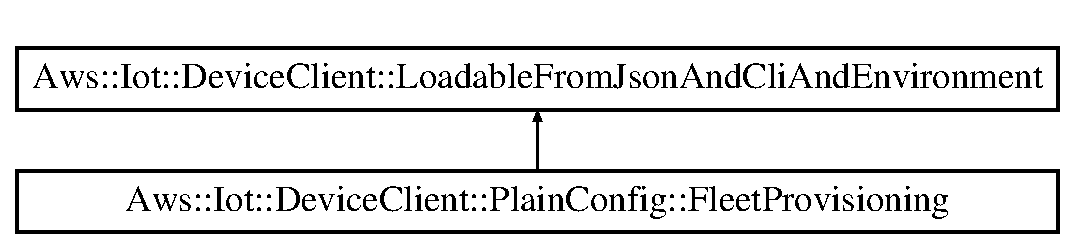
\includegraphics[height=2.000000cm]{struct_aws_1_1_iot_1_1_device_client_1_1_plain_config_1_1_fleet_provisioning}
\end{center}
\end{figure}
\doxysubsection*{Public Member Functions}
\begin{DoxyCompactItemize}
\item 
\mbox{\Hypertarget{struct_aws_1_1_iot_1_1_device_client_1_1_plain_config_1_1_fleet_provisioning_a08d5b24b9b9e6360e221b0578ca38d38}\label{struct_aws_1_1_iot_1_1_device_client_1_1_plain_config_1_1_fleet_provisioning_a08d5b24b9b9e6360e221b0578ca38d38}} 
bool {\bfseries Load\+From\+Json} (const Crt\+::\+Json\+View \&json) override
\item 
\mbox{\Hypertarget{struct_aws_1_1_iot_1_1_device_client_1_1_plain_config_1_1_fleet_provisioning_a173b6166bce025a4a7b04f0172545313}\label{struct_aws_1_1_iot_1_1_device_client_1_1_plain_config_1_1_fleet_provisioning_a173b6166bce025a4a7b04f0172545313}} 
bool {\bfseries Load\+From\+Cli\+Args} (const Cli\+Args \&cli\+Args) override
\item 
\mbox{\Hypertarget{struct_aws_1_1_iot_1_1_device_client_1_1_plain_config_1_1_fleet_provisioning_a577c310f58658f6c3f43e5239aef7d17}\label{struct_aws_1_1_iot_1_1_device_client_1_1_plain_config_1_1_fleet_provisioning_a577c310f58658f6c3f43e5239aef7d17}} 
bool {\bfseries Load\+From\+Environment} () override
\item 
\mbox{\Hypertarget{struct_aws_1_1_iot_1_1_device_client_1_1_plain_config_1_1_fleet_provisioning_a0e79dc00cd1ceb208736240a650d5004}\label{struct_aws_1_1_iot_1_1_device_client_1_1_plain_config_1_1_fleet_provisioning_a0e79dc00cd1ceb208736240a650d5004}} 
bool {\bfseries Validate} () const override
\end{DoxyCompactItemize}
\doxysubsection*{Public Attributes}
\begin{DoxyCompactItemize}
\item 
\mbox{\Hypertarget{struct_aws_1_1_iot_1_1_device_client_1_1_plain_config_1_1_fleet_provisioning_a6a563991ab2cdc06cd8cdbbfe50907f4}\label{struct_aws_1_1_iot_1_1_device_client_1_1_plain_config_1_1_fleet_provisioning_a6a563991ab2cdc06cd8cdbbfe50907f4}} 
bool {\bfseries enabled} \{false\}
\item 
\mbox{\Hypertarget{struct_aws_1_1_iot_1_1_device_client_1_1_plain_config_1_1_fleet_provisioning_a6bd9e1c7526845dba6cd792162d6a4d1}\label{struct_aws_1_1_iot_1_1_device_client_1_1_plain_config_1_1_fleet_provisioning_a6bd9e1c7526845dba6cd792162d6a4d1}} 
Aws\+::\+Crt\+::\+Optional$<$ std\+::string $>$ {\bfseries template\+Name}
\item 
\mbox{\Hypertarget{struct_aws_1_1_iot_1_1_device_client_1_1_plain_config_1_1_fleet_provisioning_a1d2fd33cc8eb1fa67f1ddccf3d1f9d6a}\label{struct_aws_1_1_iot_1_1_device_client_1_1_plain_config_1_1_fleet_provisioning_a1d2fd33cc8eb1fa67f1ddccf3d1f9d6a}} 
Aws\+::\+Crt\+::\+Optional$<$ std\+::string $>$ {\bfseries csr\+File}
\end{DoxyCompactItemize}
\doxysubsection*{Static Public Attributes}
\begin{DoxyCompactItemize}
\item 
\mbox{\Hypertarget{struct_aws_1_1_iot_1_1_device_client_1_1_plain_config_1_1_fleet_provisioning_ace3f843577e0601b349e6d764d627cc3}\label{struct_aws_1_1_iot_1_1_device_client_1_1_plain_config_1_1_fleet_provisioning_ace3f843577e0601b349e6d764d627cc3}} 
static constexpr char {\bfseries C\+L\+I\+\_\+\+E\+N\+A\+B\+L\+E\+\_\+\+F\+L\+E\+E\+T\+\_\+\+P\+R\+O\+V\+I\+S\+I\+O\+N\+I\+NG} \mbox{[}$\,$\mbox{]} = \char`\"{}-\/-\/enable-\/fleet-\/provisioning\char`\"{}
\item 
\mbox{\Hypertarget{struct_aws_1_1_iot_1_1_device_client_1_1_plain_config_1_1_fleet_provisioning_a27307f285cc3492fa57a386e9a0e0dc0}\label{struct_aws_1_1_iot_1_1_device_client_1_1_plain_config_1_1_fleet_provisioning_a27307f285cc3492fa57a386e9a0e0dc0}} 
static constexpr char {\bfseries C\+L\+I\+\_\+\+F\+L\+E\+E\+T\+\_\+\+P\+R\+O\+V\+I\+S\+I\+O\+N\+I\+N\+G\+\_\+\+T\+E\+M\+P\+L\+A\+T\+E\+\_\+\+N\+A\+ME} \mbox{[}$\,$\mbox{]} = \char`\"{}-\/-\/fleet-\/provisioning-\/template-\/name\char`\"{}
\item 
\mbox{\Hypertarget{struct_aws_1_1_iot_1_1_device_client_1_1_plain_config_1_1_fleet_provisioning_ad726b82b71fe54991fc504950e037382}\label{struct_aws_1_1_iot_1_1_device_client_1_1_plain_config_1_1_fleet_provisioning_ad726b82b71fe54991fc504950e037382}} 
static constexpr char {\bfseries C\+L\+I\+\_\+\+F\+L\+E\+E\+T\+\_\+\+P\+R\+O\+V\+I\+S\+I\+O\+N\+I\+N\+G\+\_\+\+C\+S\+R\+\_\+\+F\+I\+LE} \mbox{[}$\,$\mbox{]} = \char`\"{}-\/-\/csr-\/file\char`\"{}
\item 
\mbox{\Hypertarget{struct_aws_1_1_iot_1_1_device_client_1_1_plain_config_1_1_fleet_provisioning_a83741cd0f81dabd25027bed41f9259dc}\label{struct_aws_1_1_iot_1_1_device_client_1_1_plain_config_1_1_fleet_provisioning_a83741cd0f81dabd25027bed41f9259dc}} 
static constexpr char {\bfseries J\+S\+O\+N\+\_\+\+K\+E\+Y\+\_\+\+E\+N\+A\+B\+L\+ED} \mbox{[}$\,$\mbox{]} = \char`\"{}enabled\char`\"{}
\item 
\mbox{\Hypertarget{struct_aws_1_1_iot_1_1_device_client_1_1_plain_config_1_1_fleet_provisioning_a209b4a1c48271137b0f32ba13e5355b5}\label{struct_aws_1_1_iot_1_1_device_client_1_1_plain_config_1_1_fleet_provisioning_a209b4a1c48271137b0f32ba13e5355b5}} 
static constexpr char {\bfseries J\+S\+O\+N\+\_\+\+K\+E\+Y\+\_\+\+T\+E\+M\+P\+L\+A\+T\+E\+\_\+\+N\+A\+ME} \mbox{[}$\,$\mbox{]} = \char`\"{}template-\/name\char`\"{}
\item 
\mbox{\Hypertarget{struct_aws_1_1_iot_1_1_device_client_1_1_plain_config_1_1_fleet_provisioning_a62f3cf93a81adfe4ac579c979c0f465b}\label{struct_aws_1_1_iot_1_1_device_client_1_1_plain_config_1_1_fleet_provisioning_a62f3cf93a81adfe4ac579c979c0f465b}} 
static constexpr char {\bfseries J\+S\+O\+N\+\_\+\+K\+E\+Y\+\_\+\+C\+S\+R\+\_\+\+F\+I\+LE} \mbox{[}$\,$\mbox{]} = \char`\"{}csr-\/file\char`\"{}
\end{DoxyCompactItemize}


The documentation for this struct was generated from the following files\+:\begin{DoxyCompactItemize}
\item 
/home/runner/work/aws-\/iot-\/device-\/client/aws-\/iot-\/device-\/client/source/config/Config.\+h\item 
/home/runner/work/aws-\/iot-\/device-\/client/aws-\/iot-\/device-\/client/source/config/Config.\+cpp\end{DoxyCompactItemize}

\hypertarget{class_aws_1_1_iot_1_1_device_client_1_1_fleet_provisioning}{}\section{Aws\+:\+:Iot\+:\+:Device\+Client\+:\+:Fleet\+Provisioning Class Reference}
\label{class_aws_1_1_iot_1_1_device_client_1_1_fleet_provisioning}\index{Aws\+::\+Iot\+::\+Device\+Client\+::\+Fleet\+Provisioning@{Aws\+::\+Iot\+::\+Device\+Client\+::\+Fleet\+Provisioning}}


Provides IoT Fleet Provisioning related functionality within the Device Client.  




{\ttfamily \#include $<$Fleet\+Provisioning.\+h$>$}

\subsection*{Public Member Functions}
\begin{DoxyCompactItemize}
\item 
bool \hyperlink{class_aws_1_1_iot_1_1_device_client_1_1_fleet_provisioning_a502dc44bd8de73a21d7d42945e9b7f7b}{Provision\+Device} (std\+::shared\+\_\+ptr$<$ \hyperlink{class_aws_1_1_iot_1_1_device_client_1_1_shared_crt_resource_manager}{Shared\+Crt\+Resource\+Manager} $>$ fp\+Connection, \hyperlink{struct_aws_1_1_iot_1_1_device_client_1_1_plain_config}{Plain\+Config} \&config)
\begin{DoxyCompactList}\small\item\em Provisions device by creating and storing required resources. \end{DoxyCompactList}\end{DoxyCompactItemize}
\subsection*{Private Member Functions}
\begin{DoxyCompactItemize}
\item 
bool \hyperlink{class_aws_1_1_iot_1_1_device_client_1_1_fleet_provisioning_a9be44fae9cf49f534763243561c66586}{Create\+Certificate\+And\+Key} (Iotidentity\+::\+Iot\+Identity\+Client identity\+Client)
\begin{DoxyCompactList}\small\item\em creates a new certificate and private key using the A\+WS certificate authority \end{DoxyCompactList}\item 
bool \hyperlink{class_aws_1_1_iot_1_1_device_client_1_1_fleet_provisioning_a2044a0b21798463dff066fabbb9ad869}{Create\+Certificate\+Using\+C\+SR} (Iotidentity\+::\+Iot\+Identity\+Client identity\+Client)
\begin{DoxyCompactList}\small\item\em generate a certificate from a certificate signing request (C\+SR) that keeps user private key secure \end{DoxyCompactList}\item 
bool \hyperlink{class_aws_1_1_iot_1_1_device_client_1_1_fleet_provisioning_a2221768ad4f91ac5c593485de33c5c80}{Register\+Thing} (Iotidentity\+::\+Iot\+Identity\+Client identity\+Client)
\begin{DoxyCompactList}\small\item\em registers the device with A\+WS IoT and create cloud resources \end{DoxyCompactList}\item 
bool \hyperlink{class_aws_1_1_iot_1_1_device_client_1_1_fleet_provisioning_a6f4e107e4d2858f51603eec2f390aa96}{Export\+Runtime\+Config} (const std\+::string \&file, const std\+::string \&runtime\+Cert\+Path, const std\+::string \&runtime\+Key\+Path, const std\+::string \&runtime\+Thing\+Name)
\begin{DoxyCompactList}\small\item\em exports config of newly created resources to runtime config file \end{DoxyCompactList}\item 
bool \hyperlink{class_aws_1_1_iot_1_1_device_client_1_1_fleet_provisioning_ae209de046ed351b4c8d3ef7e1d9f00bc}{Get\+Csr\+File\+Content} (const std\+::string file\+Path)
\begin{DoxyCompactList}\small\item\em gets C\+SR file content \end{DoxyCompactList}\end{DoxyCompactItemize}
\subsection*{Private Attributes}
\begin{DoxyCompactItemize}
\item 
\mbox{\Hypertarget{class_aws_1_1_iot_1_1_device_client_1_1_fleet_provisioning_a71e0b3d04ea8e5bfcf4c1045eef3b4c1}\label{class_aws_1_1_iot_1_1_device_client_1_1_fleet_provisioning_a71e0b3d04ea8e5bfcf4c1045eef3b4c1}} 
std\+::promise$<$ bool $>$ \hyperlink{class_aws_1_1_iot_1_1_device_client_1_1_fleet_provisioning_a71e0b3d04ea8e5bfcf4c1045eef3b4c1}{keys\+Publish\+Completed\+Promise}
\begin{DoxyCompactList}\small\item\em a promise variable to check if publish request for Create\+Keys\+And\+Certificate was received \end{DoxyCompactList}\item 
\mbox{\Hypertarget{class_aws_1_1_iot_1_1_device_client_1_1_fleet_provisioning_a5c341917c25fdbf6c9401cbdd488e729}\label{class_aws_1_1_iot_1_1_device_client_1_1_fleet_provisioning_a5c341917c25fdbf6c9401cbdd488e729}} 
std\+::promise$<$ bool $>$ \hyperlink{class_aws_1_1_iot_1_1_device_client_1_1_fleet_provisioning_a5c341917c25fdbf6c9401cbdd488e729}{keys\+Accepted\+Completed\+Promise}
\begin{DoxyCompactList}\small\item\em a promise variable to check if subscription request to Create\+Keys\+And\+Certificate Accept topic was executed \end{DoxyCompactList}\item 
\mbox{\Hypertarget{class_aws_1_1_iot_1_1_device_client_1_1_fleet_provisioning_a6c49fdb1af059ea88bf99821757e6a96}\label{class_aws_1_1_iot_1_1_device_client_1_1_fleet_provisioning_a6c49fdb1af059ea88bf99821757e6a96}} 
std\+::promise$<$ bool $>$ \hyperlink{class_aws_1_1_iot_1_1_device_client_1_1_fleet_provisioning_a6c49fdb1af059ea88bf99821757e6a96}{keys\+Rejected\+Completed\+Promise}
\begin{DoxyCompactList}\small\item\em a promise variable to check if subscription to Create\+Keys\+And\+Certificate Reject topic was executed \end{DoxyCompactList}\item 
\mbox{\Hypertarget{class_aws_1_1_iot_1_1_device_client_1_1_fleet_provisioning_aafc3ae225f3d888c1439011db5393b95}\label{class_aws_1_1_iot_1_1_device_client_1_1_fleet_provisioning_aafc3ae225f3d888c1439011db5393b95}} 
std\+::promise$<$ bool $>$ \hyperlink{class_aws_1_1_iot_1_1_device_client_1_1_fleet_provisioning_aafc3ae225f3d888c1439011db5393b95}{keys\+Creation\+Completed\+Promise}
\begin{DoxyCompactList}\small\item\em a promise variable to check if publish request for Create\+Keys\+And\+Certificate was executed \end{DoxyCompactList}\item 
\mbox{\Hypertarget{class_aws_1_1_iot_1_1_device_client_1_1_fleet_provisioning_a65d4080ed16a11894450e63ec3f9ef69}\label{class_aws_1_1_iot_1_1_device_client_1_1_fleet_provisioning_a65d4080ed16a11894450e63ec3f9ef69}} 
std\+::promise$<$ bool $>$ \hyperlink{class_aws_1_1_iot_1_1_device_client_1_1_fleet_provisioning_a65d4080ed16a11894450e63ec3f9ef69}{csr\+Publish\+Completed\+Promise}
\begin{DoxyCompactList}\small\item\em a promise variable to check if publish request for Register\+Thing was received \end{DoxyCompactList}\item 
\mbox{\Hypertarget{class_aws_1_1_iot_1_1_device_client_1_1_fleet_provisioning_ad8245e3c483d250e671e5db6daf2172d}\label{class_aws_1_1_iot_1_1_device_client_1_1_fleet_provisioning_ad8245e3c483d250e671e5db6daf2172d}} 
std\+::promise$<$ bool $>$ \hyperlink{class_aws_1_1_iot_1_1_device_client_1_1_fleet_provisioning_ad8245e3c483d250e671e5db6daf2172d}{csr\+Accepted\+Completed\+Promise}
\begin{DoxyCompactList}\small\item\em a promise variable to check if subscription request to Create\+Certificate\+From\+Csr Accept topic was executed \end{DoxyCompactList}\item 
\mbox{\Hypertarget{class_aws_1_1_iot_1_1_device_client_1_1_fleet_provisioning_af12cc3b90aeaf3520c94c813fb6fc216}\label{class_aws_1_1_iot_1_1_device_client_1_1_fleet_provisioning_af12cc3b90aeaf3520c94c813fb6fc216}} 
std\+::promise$<$ bool $>$ \hyperlink{class_aws_1_1_iot_1_1_device_client_1_1_fleet_provisioning_af12cc3b90aeaf3520c94c813fb6fc216}{csr\+Rejected\+Completed\+Promise}
\begin{DoxyCompactList}\small\item\em a promise variable to check if subscription to Create\+Certificate\+From\+Csr Reject topic was executed \end{DoxyCompactList}\item 
\mbox{\Hypertarget{class_aws_1_1_iot_1_1_device_client_1_1_fleet_provisioning_ac18cad5f3af2baa69431ba0a3f8ae753}\label{class_aws_1_1_iot_1_1_device_client_1_1_fleet_provisioning_ac18cad5f3af2baa69431ba0a3f8ae753}} 
std\+::promise$<$ bool $>$ \hyperlink{class_aws_1_1_iot_1_1_device_client_1_1_fleet_provisioning_ac18cad5f3af2baa69431ba0a3f8ae753}{csr\+Creation\+Completed\+Promise}
\begin{DoxyCompactList}\small\item\em a promise variable to check if publish request for Create\+Certificate\+From\+Csr was executed \end{DoxyCompactList}\item 
\mbox{\Hypertarget{class_aws_1_1_iot_1_1_device_client_1_1_fleet_provisioning_a5f7f726a72c70311d695d859824c07d5}\label{class_aws_1_1_iot_1_1_device_client_1_1_fleet_provisioning_a5f7f726a72c70311d695d859824c07d5}} 
std\+::promise$<$ bool $>$ \hyperlink{class_aws_1_1_iot_1_1_device_client_1_1_fleet_provisioning_a5f7f726a72c70311d695d859824c07d5}{register\+Publish\+Completed\+Promise}
\begin{DoxyCompactList}\small\item\em a promise variable to check if publish request for Register\+Thing was received \end{DoxyCompactList}\item 
\mbox{\Hypertarget{class_aws_1_1_iot_1_1_device_client_1_1_fleet_provisioning_a02c6207e7109e3b3ab9a65cfb819fac4}\label{class_aws_1_1_iot_1_1_device_client_1_1_fleet_provisioning_a02c6207e7109e3b3ab9a65cfb819fac4}} 
std\+::promise$<$ bool $>$ \hyperlink{class_aws_1_1_iot_1_1_device_client_1_1_fleet_provisioning_a02c6207e7109e3b3ab9a65cfb819fac4}{register\+Accepted\+Completed\+Promise}
\begin{DoxyCompactList}\small\item\em a promise variable to check if subscription to Register\+Thing Accept topic was executed \end{DoxyCompactList}\item 
\mbox{\Hypertarget{class_aws_1_1_iot_1_1_device_client_1_1_fleet_provisioning_ac7e4a4690c0393c21ef3e9d1c83e8d15}\label{class_aws_1_1_iot_1_1_device_client_1_1_fleet_provisioning_ac7e4a4690c0393c21ef3e9d1c83e8d15}} 
std\+::promise$<$ bool $>$ \hyperlink{class_aws_1_1_iot_1_1_device_client_1_1_fleet_provisioning_ac7e4a4690c0393c21ef3e9d1c83e8d15}{register\+Rejected\+Completed\+Promise}
\begin{DoxyCompactList}\small\item\em a promise variable to check if subscription to Register\+Thing Reject topic was executed \end{DoxyCompactList}\item 
\mbox{\Hypertarget{class_aws_1_1_iot_1_1_device_client_1_1_fleet_provisioning_a1259c4a7d011bca3a473748dafc737c0}\label{class_aws_1_1_iot_1_1_device_client_1_1_fleet_provisioning_a1259c4a7d011bca3a473748dafc737c0}} 
std\+::promise$<$ bool $>$ \hyperlink{class_aws_1_1_iot_1_1_device_client_1_1_fleet_provisioning_a1259c4a7d011bca3a473748dafc737c0}{register\+Thing\+Completed\+Promise}
\begin{DoxyCompactList}\small\item\em a promise variable to check if publish request for Register\+Thing was executed \end{DoxyCompactList}\item 
\mbox{\Hypertarget{class_aws_1_1_iot_1_1_device_client_1_1_fleet_provisioning_ae0b788ac815eba2ee89dc1ace2189aba}\label{class_aws_1_1_iot_1_1_device_client_1_1_fleet_provisioning_ae0b788ac815eba2ee89dc1ace2189aba}} 
Aws\+::\+Crt\+::\+String \hyperlink{class_aws_1_1_iot_1_1_device_client_1_1_fleet_provisioning_ae0b788ac815eba2ee89dc1ace2189aba}{certificate\+Ownership\+Token}
\begin{DoxyCompactList}\small\item\em stores certificate Ownership Token \end{DoxyCompactList}\item 
\mbox{\Hypertarget{class_aws_1_1_iot_1_1_device_client_1_1_fleet_provisioning_a03535dae9cd461c763134f6bef30448d}\label{class_aws_1_1_iot_1_1_device_client_1_1_fleet_provisioning_a03535dae9cd461c763134f6bef30448d}} 
Aws\+::\+Crt\+::\+String \hyperlink{class_aws_1_1_iot_1_1_device_client_1_1_fleet_provisioning_a03535dae9cd461c763134f6bef30448d}{cert\+Path}
\begin{DoxyCompactList}\small\item\em stores certificate file path of newly created certificate \end{DoxyCompactList}\item 
\mbox{\Hypertarget{class_aws_1_1_iot_1_1_device_client_1_1_fleet_provisioning_a1ab0c65a121383574f39b48edbf06b38}\label{class_aws_1_1_iot_1_1_device_client_1_1_fleet_provisioning_a1ab0c65a121383574f39b48edbf06b38}} 
Aws\+::\+Crt\+::\+String \hyperlink{class_aws_1_1_iot_1_1_device_client_1_1_fleet_provisioning_a1ab0c65a121383574f39b48edbf06b38}{key\+Path}
\begin{DoxyCompactList}\small\item\em stores private key file path of newly created private key \end{DoxyCompactList}\item 
\mbox{\Hypertarget{class_aws_1_1_iot_1_1_device_client_1_1_fleet_provisioning_a567f7f58db121f2b5b0278321da45086}\label{class_aws_1_1_iot_1_1_device_client_1_1_fleet_provisioning_a567f7f58db121f2b5b0278321da45086}} 
std\+::string \hyperlink{class_aws_1_1_iot_1_1_device_client_1_1_fleet_provisioning_a567f7f58db121f2b5b0278321da45086}{key\+Dir} = Config\+::\+D\+E\+F\+A\+U\+L\+T\+\_\+\+K\+E\+Y\+\_\+\+D\+IR
\begin{DoxyCompactList}\small\item\em the location where keys generated by Fleet Provisioning will be stored \end{DoxyCompactList}\item 
\mbox{\Hypertarget{class_aws_1_1_iot_1_1_device_client_1_1_fleet_provisioning_a02d85e03d940ee61003b91af0a6cddf7}\label{class_aws_1_1_iot_1_1_device_client_1_1_fleet_provisioning_a02d85e03d940ee61003b91af0a6cddf7}} 
Aws\+::\+Crt\+::\+String \hyperlink{class_aws_1_1_iot_1_1_device_client_1_1_fleet_provisioning_a02d85e03d940ee61003b91af0a6cddf7}{thing\+Name}
\begin{DoxyCompactList}\small\item\em stores thing name of newly provisioned device \end{DoxyCompactList}\item 
\mbox{\Hypertarget{class_aws_1_1_iot_1_1_device_client_1_1_fleet_provisioning_a815d738dd64327e5d671119592ef7ada}\label{class_aws_1_1_iot_1_1_device_client_1_1_fleet_provisioning_a815d738dd64327e5d671119592ef7ada}} 
Aws\+::\+Crt\+::\+String \hyperlink{class_aws_1_1_iot_1_1_device_client_1_1_fleet_provisioning_a815d738dd64327e5d671119592ef7ada}{template\+Name}
\begin{DoxyCompactList}\small\item\em stores Fleet Provisioning template name \end{DoxyCompactList}\item 
\mbox{\Hypertarget{class_aws_1_1_iot_1_1_device_client_1_1_fleet_provisioning_a02873b53e68e1a63cd1087a07d795dcf}\label{class_aws_1_1_iot_1_1_device_client_1_1_fleet_provisioning_a02873b53e68e1a63cd1087a07d795dcf}} 
std\+::string \hyperlink{class_aws_1_1_iot_1_1_device_client_1_1_fleet_provisioning_a02873b53e68e1a63cd1087a07d795dcf}{csr\+File}
\begin{DoxyCompactList}\small\item\em stores C\+SR file content \end{DoxyCompactList}\end{DoxyCompactItemize}
\subsection*{Static Private Attributes}
\begin{DoxyCompactItemize}
\item 
\mbox{\Hypertarget{class_aws_1_1_iot_1_1_device_client_1_1_fleet_provisioning_adfa918ea7ce640a53fb08cd13740cfb3}\label{class_aws_1_1_iot_1_1_device_client_1_1_fleet_provisioning_adfa918ea7ce640a53fb08cd13740cfb3}} 
static constexpr char \hyperlink{class_aws_1_1_iot_1_1_device_client_1_1_fleet_provisioning_adfa918ea7ce640a53fb08cd13740cfb3}{T\+AG} \mbox{[}$\,$\mbox{]} = \char`\"{}Fleet\+Provisioning.\+cpp\char`\"{}
\begin{DoxyCompactList}\small\item\em Used by the logger to specify that log messages are coming from the Fleet Provisioning feature. \end{DoxyCompactList}\item 
\mbox{\Hypertarget{class_aws_1_1_iot_1_1_device_client_1_1_fleet_provisioning_aced71437e7c96da26a13e53288ca1247}\label{class_aws_1_1_iot_1_1_device_client_1_1_fleet_provisioning_aced71437e7c96da26a13e53288ca1247}} 
static constexpr int \hyperlink{class_aws_1_1_iot_1_1_device_client_1_1_fleet_provisioning_aced71437e7c96da26a13e53288ca1247}{D\+E\+F\+A\+U\+L\+T\+\_\+\+W\+A\+I\+T\+\_\+\+T\+I\+M\+E\+\_\+\+S\+E\+C\+O\+N\+DS} = 10
\begin{DoxyCompactList}\small\item\em The default value in seconds for which Device client will wait for promise variables to be initialized. These promise variables will be initialized in respective callback methods. \end{DoxyCompactList}\end{DoxyCompactItemize}


\subsection{Detailed Description}
Provides IoT Fleet Provisioning related functionality within the Device Client. 

\subsection{Member Function Documentation}
\mbox{\Hypertarget{class_aws_1_1_iot_1_1_device_client_1_1_fleet_provisioning_a9be44fae9cf49f534763243561c66586}\label{class_aws_1_1_iot_1_1_device_client_1_1_fleet_provisioning_a9be44fae9cf49f534763243561c66586}} 
\index{Aws\+::\+Iot\+::\+Device\+Client\+::\+Fleet\+Provisioning@{Aws\+::\+Iot\+::\+Device\+Client\+::\+Fleet\+Provisioning}!Create\+Certificate\+And\+Key@{Create\+Certificate\+And\+Key}}
\index{Create\+Certificate\+And\+Key@{Create\+Certificate\+And\+Key}!Aws\+::\+Iot\+::\+Device\+Client\+::\+Fleet\+Provisioning@{Aws\+::\+Iot\+::\+Device\+Client\+::\+Fleet\+Provisioning}}
\subsubsection{\texorpdfstring{Create\+Certificate\+And\+Key()}{CreateCertificateAndKey()}}
{\footnotesize\ttfamily bool Fleet\+Provisioning\+::\+Create\+Certificate\+And\+Key (\begin{DoxyParamCaption}\item[{Iotidentity\+::\+Iot\+Identity\+Client}]{identity\+Client }\end{DoxyParamCaption})\hspace{0.3cm}{\ttfamily [private]}}



creates a new certificate and private key using the A\+WS certificate authority 


\begin{DoxyParams}{Parameters}
{\em identity\+Client} & used for subscribing and publishing request for creating resources \\
\hline
\end{DoxyParams}
\begin{DoxyReturn}{Returns}
returns true if resources are created successfully 
\end{DoxyReturn}
\mbox{\Hypertarget{class_aws_1_1_iot_1_1_device_client_1_1_fleet_provisioning_a2044a0b21798463dff066fabbb9ad869}\label{class_aws_1_1_iot_1_1_device_client_1_1_fleet_provisioning_a2044a0b21798463dff066fabbb9ad869}} 
\index{Aws\+::\+Iot\+::\+Device\+Client\+::\+Fleet\+Provisioning@{Aws\+::\+Iot\+::\+Device\+Client\+::\+Fleet\+Provisioning}!Create\+Certificate\+Using\+C\+SR@{Create\+Certificate\+Using\+C\+SR}}
\index{Create\+Certificate\+Using\+C\+SR@{Create\+Certificate\+Using\+C\+SR}!Aws\+::\+Iot\+::\+Device\+Client\+::\+Fleet\+Provisioning@{Aws\+::\+Iot\+::\+Device\+Client\+::\+Fleet\+Provisioning}}
\subsubsection{\texorpdfstring{Create\+Certificate\+Using\+C\+S\+R()}{CreateCertificateUsingCSR()}}
{\footnotesize\ttfamily bool Fleet\+Provisioning\+::\+Create\+Certificate\+Using\+C\+SR (\begin{DoxyParamCaption}\item[{Iotidentity\+::\+Iot\+Identity\+Client}]{identity\+Client }\end{DoxyParamCaption})\hspace{0.3cm}{\ttfamily [private]}}



generate a certificate from a certificate signing request (C\+SR) that keeps user private key secure 


\begin{DoxyParams}{Parameters}
{\em identity\+Client} & used for subscribing and publishing request for creating resources \\
\hline
\end{DoxyParams}
\begin{DoxyReturn}{Returns}
returns true if resources are created successfully 
\end{DoxyReturn}
\mbox{\Hypertarget{class_aws_1_1_iot_1_1_device_client_1_1_fleet_provisioning_a6f4e107e4d2858f51603eec2f390aa96}\label{class_aws_1_1_iot_1_1_device_client_1_1_fleet_provisioning_a6f4e107e4d2858f51603eec2f390aa96}} 
\index{Aws\+::\+Iot\+::\+Device\+Client\+::\+Fleet\+Provisioning@{Aws\+::\+Iot\+::\+Device\+Client\+::\+Fleet\+Provisioning}!Export\+Runtime\+Config@{Export\+Runtime\+Config}}
\index{Export\+Runtime\+Config@{Export\+Runtime\+Config}!Aws\+::\+Iot\+::\+Device\+Client\+::\+Fleet\+Provisioning@{Aws\+::\+Iot\+::\+Device\+Client\+::\+Fleet\+Provisioning}}
\subsubsection{\texorpdfstring{Export\+Runtime\+Config()}{ExportRuntimeConfig()}}
{\footnotesize\ttfamily bool Fleet\+Provisioning\+::\+Export\+Runtime\+Config (\begin{DoxyParamCaption}\item[{const std\+::string \&}]{file,  }\item[{const std\+::string \&}]{runtime\+Cert\+Path,  }\item[{const std\+::string \&}]{runtime\+Key\+Path,  }\item[{const std\+::string \&}]{runtime\+Thing\+Name }\end{DoxyParamCaption})\hspace{0.3cm}{\ttfamily [private]}}



exports config of newly created resources to runtime config file 


\begin{DoxyParams}{Parameters}
{\em file} & runtime config file path \\
\hline
{\em runtime\+Cert\+Path} & newly created certificate file path \\
\hline
{\em runtime\+Key\+Path} & newly created private key file path \\
\hline
{\em runtime\+Thing\+Name} & thing name of newly provisioned device \\
\hline
\end{DoxyParams}
\begin{DoxyReturn}{Returns}
returns true if resources are registered and created successfully 
\end{DoxyReturn}
\mbox{\Hypertarget{class_aws_1_1_iot_1_1_device_client_1_1_fleet_provisioning_ae209de046ed351b4c8d3ef7e1d9f00bc}\label{class_aws_1_1_iot_1_1_device_client_1_1_fleet_provisioning_ae209de046ed351b4c8d3ef7e1d9f00bc}} 
\index{Aws\+::\+Iot\+::\+Device\+Client\+::\+Fleet\+Provisioning@{Aws\+::\+Iot\+::\+Device\+Client\+::\+Fleet\+Provisioning}!Get\+Csr\+File\+Content@{Get\+Csr\+File\+Content}}
\index{Get\+Csr\+File\+Content@{Get\+Csr\+File\+Content}!Aws\+::\+Iot\+::\+Device\+Client\+::\+Fleet\+Provisioning@{Aws\+::\+Iot\+::\+Device\+Client\+::\+Fleet\+Provisioning}}
\subsubsection{\texorpdfstring{Get\+Csr\+File\+Content()}{GetCsrFileContent()}}
{\footnotesize\ttfamily bool Fleet\+Provisioning\+::\+Get\+Csr\+File\+Content (\begin{DoxyParamCaption}\item[{const std\+::string}]{file\+Path }\end{DoxyParamCaption})\hspace{0.3cm}{\ttfamily [private]}}



gets C\+SR file content 


\begin{DoxyParams}{Parameters}
{\em file\+Path} & C\+SR file location \\
\hline
\end{DoxyParams}
\begin{DoxyReturn}{Returns}
returns false if client is not able to open the file or if file is empty 
\end{DoxyReturn}
\mbox{\Hypertarget{class_aws_1_1_iot_1_1_device_client_1_1_fleet_provisioning_a502dc44bd8de73a21d7d42945e9b7f7b}\label{class_aws_1_1_iot_1_1_device_client_1_1_fleet_provisioning_a502dc44bd8de73a21d7d42945e9b7f7b}} 
\index{Aws\+::\+Iot\+::\+Device\+Client\+::\+Fleet\+Provisioning@{Aws\+::\+Iot\+::\+Device\+Client\+::\+Fleet\+Provisioning}!Provision\+Device@{Provision\+Device}}
\index{Provision\+Device@{Provision\+Device}!Aws\+::\+Iot\+::\+Device\+Client\+::\+Fleet\+Provisioning@{Aws\+::\+Iot\+::\+Device\+Client\+::\+Fleet\+Provisioning}}
\subsubsection{\texorpdfstring{Provision\+Device()}{ProvisionDevice()}}
{\footnotesize\ttfamily bool Fleet\+Provisioning\+::\+Provision\+Device (\begin{DoxyParamCaption}\item[{std\+::shared\+\_\+ptr$<$ \hyperlink{class_aws_1_1_iot_1_1_device_client_1_1_shared_crt_resource_manager}{Shared\+Crt\+Resource\+Manager} $>$}]{fp\+Connection,  }\item[{\hyperlink{struct_aws_1_1_iot_1_1_device_client_1_1_plain_config}{Plain\+Config} \&}]{config }\end{DoxyParamCaption})}



Provisions device by creating and storing required resources. 


\begin{DoxyParams}{Parameters}
{\em fp\+Connection} & the Mqtt\+Connection\+Manager \\
\hline
{\em config} & configuration information passed in by the user via either the command line or configuration file \\
\hline
\end{DoxyParams}
\begin{DoxyReturn}{Returns}
returns true if device is provisioned successfully 
\end{DoxyReturn}
\mbox{\Hypertarget{class_aws_1_1_iot_1_1_device_client_1_1_fleet_provisioning_a2221768ad4f91ac5c593485de33c5c80}\label{class_aws_1_1_iot_1_1_device_client_1_1_fleet_provisioning_a2221768ad4f91ac5c593485de33c5c80}} 
\index{Aws\+::\+Iot\+::\+Device\+Client\+::\+Fleet\+Provisioning@{Aws\+::\+Iot\+::\+Device\+Client\+::\+Fleet\+Provisioning}!Register\+Thing@{Register\+Thing}}
\index{Register\+Thing@{Register\+Thing}!Aws\+::\+Iot\+::\+Device\+Client\+::\+Fleet\+Provisioning@{Aws\+::\+Iot\+::\+Device\+Client\+::\+Fleet\+Provisioning}}
\subsubsection{\texorpdfstring{Register\+Thing()}{RegisterThing()}}
{\footnotesize\ttfamily bool Fleet\+Provisioning\+::\+Register\+Thing (\begin{DoxyParamCaption}\item[{Iotidentity\+::\+Iot\+Identity\+Client}]{identity\+Client }\end{DoxyParamCaption})\hspace{0.3cm}{\ttfamily [private]}}



registers the device with A\+WS IoT and create cloud resources 


\begin{DoxyParams}{Parameters}
{\em identity\+Client} & used for subscribing and publishing request for registering and creating resources \\
\hline
\end{DoxyParams}
\begin{DoxyReturn}{Returns}
returns true if resources are registered and created successfully 
\end{DoxyReturn}


The documentation for this class was generated from the following files\+:\begin{DoxyCompactItemize}
\item 
/home/\+A\+N\+T.\+A\+M\+A\+Z\+O\+N.\+C\+O\+M/lwwilkov/\+Workspace/aws-\/iot-\/device-\/client/source/fleetprovisioning/Fleet\+Provisioning.\+h\item 
/home/\+A\+N\+T.\+A\+M\+A\+Z\+O\+N.\+C\+O\+M/lwwilkov/\+Workspace/aws-\/iot-\/device-\/client/source/fleetprovisioning/Fleet\+Provisioning.\+cpp\end{DoxyCompactItemize}

\hypertarget{struct_aws_1_1_iot_1_1_device_client_1_1_plain_config_1_1_fleet_provisioning_runtime_config}{}\doxysection{Aws\+::Iot\+::Device\+Client\+::Plain\+Config\+::Fleet\+Provisioning\+Runtime\+Config Struct Reference}
\label{struct_aws_1_1_iot_1_1_device_client_1_1_plain_config_1_1_fleet_provisioning_runtime_config}\index{Aws::Iot::DeviceClient::PlainConfig::FleetProvisioningRuntimeConfig@{Aws::Iot::DeviceClient::PlainConfig::FleetProvisioningRuntimeConfig}}
Inheritance diagram for Aws\+::Iot\+::Device\+Client\+::Plain\+Config\+::Fleet\+Provisioning\+Runtime\+Config\+:\begin{figure}[H]
\begin{center}
\leavevmode
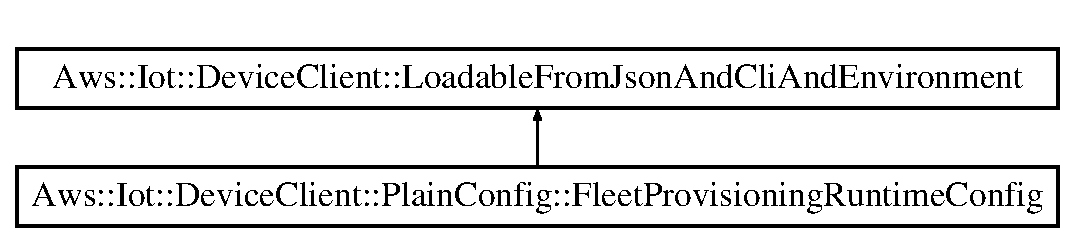
\includegraphics[height=2.000000cm]{struct_aws_1_1_iot_1_1_device_client_1_1_plain_config_1_1_fleet_provisioning_runtime_config}
\end{center}
\end{figure}
\doxysubsection*{Public Member Functions}
\begin{DoxyCompactItemize}
\item 
\mbox{\Hypertarget{struct_aws_1_1_iot_1_1_device_client_1_1_plain_config_1_1_fleet_provisioning_runtime_config_a12642dac957ddf8cc299248af3fffaf7}\label{struct_aws_1_1_iot_1_1_device_client_1_1_plain_config_1_1_fleet_provisioning_runtime_config_a12642dac957ddf8cc299248af3fffaf7}} 
bool {\bfseries Load\+From\+Json} (const Crt\+::\+Json\+View \&json) override
\item 
\mbox{\Hypertarget{struct_aws_1_1_iot_1_1_device_client_1_1_plain_config_1_1_fleet_provisioning_runtime_config_a17ed50833febbd764efbc961f21ae95a}\label{struct_aws_1_1_iot_1_1_device_client_1_1_plain_config_1_1_fleet_provisioning_runtime_config_a17ed50833febbd764efbc961f21ae95a}} 
bool {\bfseries Load\+From\+Cli\+Args} (const Cli\+Args \&cli\+Args) override
\item 
\mbox{\Hypertarget{struct_aws_1_1_iot_1_1_device_client_1_1_plain_config_1_1_fleet_provisioning_runtime_config_a59e7de2571c11de4b0d34eed2fa41658}\label{struct_aws_1_1_iot_1_1_device_client_1_1_plain_config_1_1_fleet_provisioning_runtime_config_a59e7de2571c11de4b0d34eed2fa41658}} 
bool {\bfseries Load\+From\+Environment} () override
\item 
\mbox{\Hypertarget{struct_aws_1_1_iot_1_1_device_client_1_1_plain_config_1_1_fleet_provisioning_runtime_config_a052642641fb1331492d918b9f715252d}\label{struct_aws_1_1_iot_1_1_device_client_1_1_plain_config_1_1_fleet_provisioning_runtime_config_a052642641fb1331492d918b9f715252d}} 
bool {\bfseries Validate} () const override
\end{DoxyCompactItemize}
\doxysubsection*{Public Attributes}
\begin{DoxyCompactItemize}
\item 
\mbox{\Hypertarget{struct_aws_1_1_iot_1_1_device_client_1_1_plain_config_1_1_fleet_provisioning_runtime_config_a1c516ec9ce10ed2fc6541a5d7440444c}\label{struct_aws_1_1_iot_1_1_device_client_1_1_plain_config_1_1_fleet_provisioning_runtime_config_a1c516ec9ce10ed2fc6541a5d7440444c}} 
bool {\bfseries completed\+Fleet\+Provisioning} \{false\}
\item 
\mbox{\Hypertarget{struct_aws_1_1_iot_1_1_device_client_1_1_plain_config_1_1_fleet_provisioning_runtime_config_a6b663b7927345ac5b9fec57db39f03d2}\label{struct_aws_1_1_iot_1_1_device_client_1_1_plain_config_1_1_fleet_provisioning_runtime_config_a6b663b7927345ac5b9fec57db39f03d2}} 
Aws\+::\+Crt\+::\+Optional$<$ std\+::string $>$ {\bfseries cert}
\item 
\mbox{\Hypertarget{struct_aws_1_1_iot_1_1_device_client_1_1_plain_config_1_1_fleet_provisioning_runtime_config_a46e3ed0a0cac505917eeaec31a3a23ce}\label{struct_aws_1_1_iot_1_1_device_client_1_1_plain_config_1_1_fleet_provisioning_runtime_config_a46e3ed0a0cac505917eeaec31a3a23ce}} 
Aws\+::\+Crt\+::\+Optional$<$ std\+::string $>$ {\bfseries key}
\item 
\mbox{\Hypertarget{struct_aws_1_1_iot_1_1_device_client_1_1_plain_config_1_1_fleet_provisioning_runtime_config_a75cc939343591f3017ce08f6b3a97209}\label{struct_aws_1_1_iot_1_1_device_client_1_1_plain_config_1_1_fleet_provisioning_runtime_config_a75cc939343591f3017ce08f6b3a97209}} 
Aws\+::\+Crt\+::\+Optional$<$ std\+::string $>$ {\bfseries thing\+Name}
\end{DoxyCompactItemize}
\doxysubsection*{Static Public Attributes}
\begin{DoxyCompactItemize}
\item 
\mbox{\Hypertarget{struct_aws_1_1_iot_1_1_device_client_1_1_plain_config_1_1_fleet_provisioning_runtime_config_ac0349fbd3e9674b200f2ad12b72b99c9}\label{struct_aws_1_1_iot_1_1_device_client_1_1_plain_config_1_1_fleet_provisioning_runtime_config_ac0349fbd3e9674b200f2ad12b72b99c9}} 
static constexpr char {\bfseries J\+S\+O\+N\+\_\+\+K\+E\+Y\+\_\+\+C\+O\+M\+P\+L\+E\+T\+E\+D\+\_\+\+F\+L\+E\+E\+T\+\_\+\+P\+R\+O\+V\+I\+S\+I\+O\+N\+I\+NG} \mbox{[}$\,$\mbox{]} = \char`\"{}completed-\/fp\char`\"{}
\item 
\mbox{\Hypertarget{struct_aws_1_1_iot_1_1_device_client_1_1_plain_config_1_1_fleet_provisioning_runtime_config_a75abbf312bb769b69e9d921e7f018027}\label{struct_aws_1_1_iot_1_1_device_client_1_1_plain_config_1_1_fleet_provisioning_runtime_config_a75abbf312bb769b69e9d921e7f018027}} 
static constexpr char {\bfseries J\+S\+O\+N\+\_\+\+K\+E\+Y\+\_\+\+C\+E\+RT} \mbox{[}$\,$\mbox{]} = \char`\"{}cert\char`\"{}
\item 
\mbox{\Hypertarget{struct_aws_1_1_iot_1_1_device_client_1_1_plain_config_1_1_fleet_provisioning_runtime_config_a9936969e5d2ad49ee0c7950cf765abcb}\label{struct_aws_1_1_iot_1_1_device_client_1_1_plain_config_1_1_fleet_provisioning_runtime_config_a9936969e5d2ad49ee0c7950cf765abcb}} 
static constexpr char {\bfseries J\+S\+O\+N\+\_\+\+K\+E\+Y\+\_\+\+K\+EY} \mbox{[}$\,$\mbox{]} = \char`\"{}key\char`\"{}
\item 
\mbox{\Hypertarget{struct_aws_1_1_iot_1_1_device_client_1_1_plain_config_1_1_fleet_provisioning_runtime_config_a0f9b8beba633c2ce59f50f043bbe71c6}\label{struct_aws_1_1_iot_1_1_device_client_1_1_plain_config_1_1_fleet_provisioning_runtime_config_a0f9b8beba633c2ce59f50f043bbe71c6}} 
static constexpr char {\bfseries J\+S\+O\+N\+\_\+\+K\+E\+Y\+\_\+\+T\+H\+I\+N\+G\+\_\+\+N\+A\+ME} \mbox{[}$\,$\mbox{]} = \char`\"{}thing-\/name\char`\"{}
\end{DoxyCompactItemize}


The documentation for this struct was generated from the following files\+:\begin{DoxyCompactItemize}
\item 
/home/runner/work/aws-\/iot-\/device-\/client/aws-\/iot-\/device-\/client/source/config/Config.\+h\item 
/home/runner/work/aws-\/iot-\/device-\/client/aws-\/iot-\/device-\/client/source/config/Config.\+cpp\end{DoxyCompactItemize}

\hypertarget{class_aws_1_1_iot_1_1_device_client_1_1_jobs_1_1_job_engine}{}\section{Aws\+:\+:Iot\+:\+:Device\+Client\+:\+:Jobs\+:\+:Job\+Engine Class Reference}
\label{class_aws_1_1_iot_1_1_device_client_1_1_jobs_1_1_job_engine}\index{Aws\+::\+Iot\+::\+Device\+Client\+::\+Jobs\+::\+Job\+Engine@{Aws\+::\+Iot\+::\+Device\+Client\+::\+Jobs\+::\+Job\+Engine}}


Manages the execution of a Job.  




{\ttfamily \#include $<$Job\+Engine.\+h$>$}

\subsection*{Public Member Functions}
\begin{DoxyCompactItemize}
\item 
void \hyperlink{class_aws_1_1_iot_1_1_device_client_1_1_jobs_1_1_job_engine_aab65000d16ffe1c250c9af0c51d9abe6}{process\+Cmd\+Output} (int fd, bool is\+Std\+Err, int child\+P\+ID)
\begin{DoxyCompactList}\small\item\em Used by output processing threads to assess output from the child process. \end{DoxyCompactList}\item 
int \hyperlink{class_aws_1_1_iot_1_1_device_client_1_1_jobs_1_1_job_engine_a51fcb47a9ed2d8c32109d47cc4cfff6d}{exec\+\_\+cmd} (std\+::string action, std\+::vector$<$ std\+::string $>$ args)
\begin{DoxyCompactList}\small\item\em Executes the given command (action) and passes the provided vector of arguments to that command. \end{DoxyCompactList}\item 
int \hyperlink{class_aws_1_1_iot_1_1_device_client_1_1_jobs_1_1_job_engine_abcc11a86226e74648e3a5395ae180171}{has\+Errors} ()
\begin{DoxyCompactList}\small\item\em Begin the execution of a command with the specified arguments. \end{DoxyCompactList}\item 
std\+::string \hyperlink{class_aws_1_1_iot_1_1_device_client_1_1_jobs_1_1_job_engine_affcb240c8fd6c1fe197997131929c20e}{get\+Std\+Out} ()
\begin{DoxyCompactList}\small\item\em Take the S\+T\+D\+O\+UT received from the child process. \end{DoxyCompactList}\item 
std\+::string \hyperlink{class_aws_1_1_iot_1_1_device_client_1_1_jobs_1_1_job_engine_a2f3764967a7d06f30fe7e3df583b5040}{get\+Std\+Err} ()
\begin{DoxyCompactList}\small\item\em Take the S\+T\+D\+E\+RR received from the child process. \end{DoxyCompactList}\end{DoxyCompactItemize}
\subsection*{Private Attributes}
\begin{DoxyCompactItemize}
\item 
\mbox{\Hypertarget{class_aws_1_1_iot_1_1_device_client_1_1_jobs_1_1_job_engine_a3e391a699bb7c903498eead712a20288}\label{class_aws_1_1_iot_1_1_device_client_1_1_jobs_1_1_job_engine_a3e391a699bb7c903498eead712a20288}} 
const char $\ast$ {\bfseries T\+AG} = \char`\"{}Job\+Engine.\+cpp\char`\"{}
\item 
std\+::atomic\+\_\+int \hyperlink{class_aws_1_1_iot_1_1_device_client_1_1_jobs_1_1_job_engine_a1cac8361d8365feb7b0e5807abc07e33}{errors} \{0\}
\begin{DoxyCompactList}\small\item\em The number of lines received on S\+T\+D\+E\+RR from the child process. \end{DoxyCompactList}\item 
\mbox{\Hypertarget{class_aws_1_1_iot_1_1_device_client_1_1_jobs_1_1_job_engine_ac90bc5fc6289d89cb012f0d6322b520c}\label{class_aws_1_1_iot_1_1_device_client_1_1_jobs_1_1_job_engine_ac90bc5fc6289d89cb012f0d6322b520c}} 
\hyperlink{class_aws_1_1_iot_1_1_device_client_1_1_jobs_1_1_limited_stream_buffer}{Aws\+::\+Iot\+::\+Device\+Client\+::\+Jobs\+::\+Limited\+Stream\+Buffer} \hyperlink{class_aws_1_1_iot_1_1_device_client_1_1_jobs_1_1_job_engine_ac90bc5fc6289d89cb012f0d6322b520c}{stdoutstream}
\begin{DoxyCompactList}\small\item\em Partial output from S\+T\+D\+O\+UT of the child process to be used in Update\+Job\+Execution. \end{DoxyCompactList}\item 
\mbox{\Hypertarget{class_aws_1_1_iot_1_1_device_client_1_1_jobs_1_1_job_engine_aefc97336f6335fb64a11ee690c22d834}\label{class_aws_1_1_iot_1_1_device_client_1_1_jobs_1_1_job_engine_aefc97336f6335fb64a11ee690c22d834}} 
\hyperlink{class_aws_1_1_iot_1_1_device_client_1_1_jobs_1_1_limited_stream_buffer}{Aws\+::\+Iot\+::\+Device\+Client\+::\+Jobs\+::\+Limited\+Stream\+Buffer} \hyperlink{class_aws_1_1_iot_1_1_device_client_1_1_jobs_1_1_job_engine_aefc97336f6335fb64a11ee690c22d834}{stderrstream}
\begin{DoxyCompactList}\small\item\em Partial output from S\+T\+D\+E\+RR of the child process to be used in Update\+Job\+Execution. \end{DoxyCompactList}\end{DoxyCompactItemize}
\subsection*{Static Private Attributes}
\begin{DoxyCompactItemize}
\item 
\mbox{\Hypertarget{class_aws_1_1_iot_1_1_device_client_1_1_jobs_1_1_job_engine_a333eb4a7c9d0ec7143e2b954ee5a1be3}\label{class_aws_1_1_iot_1_1_device_client_1_1_jobs_1_1_job_engine_a333eb4a7c9d0ec7143e2b954ee5a1be3}} 
static constexpr size\+\_\+t \hyperlink{class_aws_1_1_iot_1_1_device_client_1_1_jobs_1_1_job_engine_a333eb4a7c9d0ec7143e2b954ee5a1be3}{M\+A\+X\+\_\+\+L\+O\+G\+\_\+\+L\+I\+N\+ES} = 1000
\begin{DoxyCompactList}\small\item\em The maximum number of lines that we\textquotesingle{}ll read from S\+T\+D\+O\+UT or S\+T\+D\+E\+RR of the child process before stopping. This prevents against log corruption in the event that the specified job generates a large volume of output. \end{DoxyCompactList}\end{DoxyCompactItemize}


\subsection{Detailed Description}
Manages the execution of a Job. 

The \hyperlink{class_aws_1_1_iot_1_1_device_client_1_1_jobs_1_1_job_engine}{Job\+Engine} is fully responsible for executing a given command and its arguments, which may point to handlers provided as part of the Device Client or to other executables available to the device. The \hyperlink{class_aws_1_1_iot_1_1_device_client_1_1_jobs_1_1_job_engine}{Job\+Engine} manages all of the setup required to redirect output from the child process so that it can be analyzed by the Jobs feature and used to determine job success. 

\subsection{Member Function Documentation}
\mbox{\Hypertarget{class_aws_1_1_iot_1_1_device_client_1_1_jobs_1_1_job_engine_a51fcb47a9ed2d8c32109d47cc4cfff6d}\label{class_aws_1_1_iot_1_1_device_client_1_1_jobs_1_1_job_engine_a51fcb47a9ed2d8c32109d47cc4cfff6d}} 
\index{Aws\+::\+Iot\+::\+Device\+Client\+::\+Jobs\+::\+Job\+Engine@{Aws\+::\+Iot\+::\+Device\+Client\+::\+Jobs\+::\+Job\+Engine}!exec\+\_\+cmd@{exec\+\_\+cmd}}
\index{exec\+\_\+cmd@{exec\+\_\+cmd}!Aws\+::\+Iot\+::\+Device\+Client\+::\+Jobs\+::\+Job\+Engine@{Aws\+::\+Iot\+::\+Device\+Client\+::\+Jobs\+::\+Job\+Engine}}
\subsubsection{\texorpdfstring{exec\+\_\+cmd()}{exec\_cmd()}}
{\footnotesize\ttfamily int Job\+Engine\+::exec\+\_\+cmd (\begin{DoxyParamCaption}\item[{std\+::string}]{action,  }\item[{std\+::vector$<$ std\+::string $>$}]{args }\end{DoxyParamCaption})}



Executes the given command (action) and passes the provided vector of arguments to that command. 


\begin{DoxyParams}{Parameters}
{\em action} & the command to execute \\
\hline
{\em args} & the arguments to pass to that command \\
\hline
\end{DoxyParams}
\begin{DoxyReturn}{Returns}
an integer representing the return code of the executed process 
\end{DoxyReturn}
\mbox{\Hypertarget{class_aws_1_1_iot_1_1_device_client_1_1_jobs_1_1_job_engine_a2f3764967a7d06f30fe7e3df583b5040}\label{class_aws_1_1_iot_1_1_device_client_1_1_jobs_1_1_job_engine_a2f3764967a7d06f30fe7e3df583b5040}} 
\index{Aws\+::\+Iot\+::\+Device\+Client\+::\+Jobs\+::\+Job\+Engine@{Aws\+::\+Iot\+::\+Device\+Client\+::\+Jobs\+::\+Job\+Engine}!get\+Std\+Err@{get\+Std\+Err}}
\index{get\+Std\+Err@{get\+Std\+Err}!Aws\+::\+Iot\+::\+Device\+Client\+::\+Jobs\+::\+Job\+Engine@{Aws\+::\+Iot\+::\+Device\+Client\+::\+Jobs\+::\+Job\+Engine}}
\subsubsection{\texorpdfstring{get\+Std\+Err()}{getStdErr()}}
{\footnotesize\ttfamily std\+::string Aws\+::\+Iot\+::\+Device\+Client\+::\+Jobs\+::\+Job\+Engine\+::get\+Std\+Err (\begin{DoxyParamCaption}{ }\end{DoxyParamCaption})\hspace{0.3cm}{\ttfamily [inline]}}



Take the S\+T\+D\+E\+RR received from the child process. 

\begin{DoxyReturn}{Returns}
a \hyperlink{class_aws_1_1_iot_1_1_device_client_1_1_jobs_1_1_limited_stream_buffer}{Limited\+Stream\+Buffer} taken from the \hyperlink{class_aws_1_1_iot_1_1_device_client_1_1_jobs_1_1_job_engine}{Job\+Engine} 
\end{DoxyReturn}
\mbox{\Hypertarget{class_aws_1_1_iot_1_1_device_client_1_1_jobs_1_1_job_engine_affcb240c8fd6c1fe197997131929c20e}\label{class_aws_1_1_iot_1_1_device_client_1_1_jobs_1_1_job_engine_affcb240c8fd6c1fe197997131929c20e}} 
\index{Aws\+::\+Iot\+::\+Device\+Client\+::\+Jobs\+::\+Job\+Engine@{Aws\+::\+Iot\+::\+Device\+Client\+::\+Jobs\+::\+Job\+Engine}!get\+Std\+Out@{get\+Std\+Out}}
\index{get\+Std\+Out@{get\+Std\+Out}!Aws\+::\+Iot\+::\+Device\+Client\+::\+Jobs\+::\+Job\+Engine@{Aws\+::\+Iot\+::\+Device\+Client\+::\+Jobs\+::\+Job\+Engine}}
\subsubsection{\texorpdfstring{get\+Std\+Out()}{getStdOut()}}
{\footnotesize\ttfamily std\+::string Aws\+::\+Iot\+::\+Device\+Client\+::\+Jobs\+::\+Job\+Engine\+::get\+Std\+Out (\begin{DoxyParamCaption}{ }\end{DoxyParamCaption})\hspace{0.3cm}{\ttfamily [inline]}}



Take the S\+T\+D\+O\+UT received from the child process. 

\begin{DoxyReturn}{Returns}
a \hyperlink{class_aws_1_1_iot_1_1_device_client_1_1_jobs_1_1_limited_stream_buffer}{Limited\+Stream\+Buffer} taken from the \hyperlink{class_aws_1_1_iot_1_1_device_client_1_1_jobs_1_1_job_engine}{Job\+Engine} 
\end{DoxyReturn}
\mbox{\Hypertarget{class_aws_1_1_iot_1_1_device_client_1_1_jobs_1_1_job_engine_abcc11a86226e74648e3a5395ae180171}\label{class_aws_1_1_iot_1_1_device_client_1_1_jobs_1_1_job_engine_abcc11a86226e74648e3a5395ae180171}} 
\index{Aws\+::\+Iot\+::\+Device\+Client\+::\+Jobs\+::\+Job\+Engine@{Aws\+::\+Iot\+::\+Device\+Client\+::\+Jobs\+::\+Job\+Engine}!has\+Errors@{has\+Errors}}
\index{has\+Errors@{has\+Errors}!Aws\+::\+Iot\+::\+Device\+Client\+::\+Jobs\+::\+Job\+Engine@{Aws\+::\+Iot\+::\+Device\+Client\+::\+Jobs\+::\+Job\+Engine}}
\subsubsection{\texorpdfstring{has\+Errors()}{hasErrors()}}
{\footnotesize\ttfamily int Aws\+::\+Iot\+::\+Device\+Client\+::\+Jobs\+::\+Job\+Engine\+::has\+Errors (\begin{DoxyParamCaption}{ }\end{DoxyParamCaption})\hspace{0.3cm}{\ttfamily [inline]}}



Begin the execution of a command with the specified arguments. 


\begin{DoxyParams}{Parameters}
{\em operation} & the operation to perform, likely the path to an executable \\
\hline
{\em args} & the arguments to pass to the executable \\
\hline
\end{DoxyParams}
\begin{DoxyReturn}{Returns}
the return code of the child process, or an error code if it cannot be executed Whether the \hyperlink{class_aws_1_1_iot_1_1_device_client_1_1_jobs_1_1_job_engine}{Job\+Engine} is reporting errors received from the child process

an integer representing the number of lines received on S\+T\+D\+E\+RR 
\end{DoxyReturn}
\mbox{\Hypertarget{class_aws_1_1_iot_1_1_device_client_1_1_jobs_1_1_job_engine_aab65000d16ffe1c250c9af0c51d9abe6}\label{class_aws_1_1_iot_1_1_device_client_1_1_jobs_1_1_job_engine_aab65000d16ffe1c250c9af0c51d9abe6}} 
\index{Aws\+::\+Iot\+::\+Device\+Client\+::\+Jobs\+::\+Job\+Engine@{Aws\+::\+Iot\+::\+Device\+Client\+::\+Jobs\+::\+Job\+Engine}!process\+Cmd\+Output@{process\+Cmd\+Output}}
\index{process\+Cmd\+Output@{process\+Cmd\+Output}!Aws\+::\+Iot\+::\+Device\+Client\+::\+Jobs\+::\+Job\+Engine@{Aws\+::\+Iot\+::\+Device\+Client\+::\+Jobs\+::\+Job\+Engine}}
\subsubsection{\texorpdfstring{process\+Cmd\+Output()}{processCmdOutput()}}
{\footnotesize\ttfamily void Job\+Engine\+::process\+Cmd\+Output (\begin{DoxyParamCaption}\item[{int}]{fd,  }\item[{bool}]{is\+Std\+Err,  }\item[{int}]{child\+P\+ID }\end{DoxyParamCaption})}



Used by output processing threads to assess output from the child process. 


\begin{DoxyParams}{Parameters}
{\em fd} & the file descriptor of the output to process \\
\hline
{\em is\+Std\+Err} & whether the output being processed is from S\+T\+D\+E\+RR \\
\hline
{\em child\+P\+ID} & the process ID of the child process \\
\hline
\end{DoxyParams}


\subsection{Member Data Documentation}
\mbox{\Hypertarget{class_aws_1_1_iot_1_1_device_client_1_1_jobs_1_1_job_engine_a1cac8361d8365feb7b0e5807abc07e33}\label{class_aws_1_1_iot_1_1_device_client_1_1_jobs_1_1_job_engine_a1cac8361d8365feb7b0e5807abc07e33}} 
\index{Aws\+::\+Iot\+::\+Device\+Client\+::\+Jobs\+::\+Job\+Engine@{Aws\+::\+Iot\+::\+Device\+Client\+::\+Jobs\+::\+Job\+Engine}!errors@{errors}}
\index{errors@{errors}!Aws\+::\+Iot\+::\+Device\+Client\+::\+Jobs\+::\+Job\+Engine@{Aws\+::\+Iot\+::\+Device\+Client\+::\+Jobs\+::\+Job\+Engine}}
\subsubsection{\texorpdfstring{errors}{errors}}
{\footnotesize\ttfamily std\+::atomic\+\_\+int Aws\+::\+Iot\+::\+Device\+Client\+::\+Jobs\+::\+Job\+Engine\+::errors \{0\}\hspace{0.3cm}{\ttfamily [private]}}



The number of lines received on S\+T\+D\+E\+RR from the child process. 

Used to determine whether the job was successful or not, since a script with multiple commands will return the return code of the final command and may not be indicative of whether all actions were successful. The incoming job document may include a property that specifies an acceptable number of S\+T\+D\+E\+RR lines to allow in case some errors are expected. 

The documentation for this class was generated from the following files\+:\begin{DoxyCompactItemize}
\item 
/home/\+A\+N\+T.\+A\+M\+A\+Z\+O\+N.\+C\+O\+M/lwwilkov/\+Workspace/aws-\/iot-\/device-\/client/source/jobs/Job\+Engine.\+h\item 
/home/\+A\+N\+T.\+A\+M\+A\+Z\+O\+N.\+C\+O\+M/lwwilkov/\+Workspace/aws-\/iot-\/device-\/client/source/jobs/Job\+Engine.\+cpp\end{DoxyCompactItemize}

\hypertarget{struct_aws_1_1_iot_1_1_device_client_1_1_jobs_1_1_jobs_feature_1_1_job_execution_status_info}{}\doxysection{Aws\+::Iot\+::Device\+Client\+::Jobs\+::Jobs\+Feature\+::Job\+Execution\+Status\+Info Struct Reference}
\label{struct_aws_1_1_iot_1_1_device_client_1_1_jobs_1_1_jobs_feature_1_1_job_execution_status_info}\index{Aws::Iot::DeviceClient::Jobs::JobsFeature::JobExecutionStatusInfo@{Aws::Iot::DeviceClient::Jobs::JobsFeature::JobExecutionStatusInfo}}


Wrapper struct to aggregate \mbox{\hyperlink{class_aws_1_1_iot_1_1_device_client_1_1_jobs_1_1_job_engine}{Job\+Engine}} output for updating a job execution status.  


\doxysubsection*{Public Attributes}
\begin{DoxyCompactItemize}
\item 
\mbox{\Hypertarget{struct_aws_1_1_iot_1_1_device_client_1_1_jobs_1_1_jobs_feature_1_1_job_execution_status_info_aae5af48be2dc11c257070b17b81ca123}\label{struct_aws_1_1_iot_1_1_device_client_1_1_jobs_1_1_jobs_feature_1_1_job_execution_status_info_aae5af48be2dc11c257070b17b81ca123}} 
Aws\+::\+Iotjobs\+::\+Job\+Status {\bfseries status}
\item 
\mbox{\Hypertarget{struct_aws_1_1_iot_1_1_device_client_1_1_jobs_1_1_jobs_feature_1_1_job_execution_status_info_aaad8e97a7c1adf33e3037e7ff9594c99}\label{struct_aws_1_1_iot_1_1_device_client_1_1_jobs_1_1_jobs_feature_1_1_job_execution_status_info_aaad8e97a7c1adf33e3037e7ff9594c99}} 
std\+::string {\bfseries reason}
\item 
\mbox{\Hypertarget{struct_aws_1_1_iot_1_1_device_client_1_1_jobs_1_1_jobs_feature_1_1_job_execution_status_info_aa1ada87fdda714692b2e6de1ab6417a5}\label{struct_aws_1_1_iot_1_1_device_client_1_1_jobs_1_1_jobs_feature_1_1_job_execution_status_info_aa1ada87fdda714692b2e6de1ab6417a5}} 
std\+::string {\bfseries stdoutput}
\item 
\mbox{\Hypertarget{struct_aws_1_1_iot_1_1_device_client_1_1_jobs_1_1_jobs_feature_1_1_job_execution_status_info_a83681cf08133b927d3ae489f26343a66}\label{struct_aws_1_1_iot_1_1_device_client_1_1_jobs_1_1_jobs_feature_1_1_job_execution_status_info_a83681cf08133b927d3ae489f26343a66}} 
std\+::string {\bfseries stderror}
\end{DoxyCompactItemize}


\doxysubsection{Detailed Description}
Wrapper struct to aggregate \mbox{\hyperlink{class_aws_1_1_iot_1_1_device_client_1_1_jobs_1_1_job_engine}{Job\+Engine}} output for updating a job execution status. 

The documentation for this struct was generated from the following file\+:\begin{DoxyCompactItemize}
\item 
/home/runner/work/aws-\/iot-\/device-\/client/aws-\/iot-\/device-\/client/source/jobs/Jobs\+Feature.\+h\end{DoxyCompactItemize}

\hypertarget{struct_aws_1_1_iot_1_1_device_client_1_1_plain_config_1_1_jobs}{}\section{Aws\+:\+:Iot\+:\+:Device\+Client\+:\+:Plain\+Config\+:\+:Jobs Struct Reference}
\label{struct_aws_1_1_iot_1_1_device_client_1_1_plain_config_1_1_jobs}\index{Aws\+::\+Iot\+::\+Device\+Client\+::\+Plain\+Config\+::\+Jobs@{Aws\+::\+Iot\+::\+Device\+Client\+::\+Plain\+Config\+::\+Jobs}}
Inheritance diagram for Aws\+:\+:Iot\+:\+:Device\+Client\+:\+:Plain\+Config\+:\+:Jobs\+:\begin{figure}[H]
\begin{center}
\leavevmode
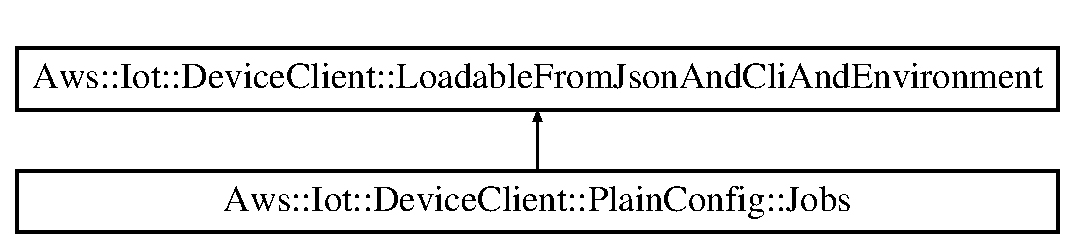
\includegraphics[height=2.000000cm]{struct_aws_1_1_iot_1_1_device_client_1_1_plain_config_1_1_jobs}
\end{center}
\end{figure}
\subsection*{Public Member Functions}
\begin{DoxyCompactItemize}
\item 
\mbox{\Hypertarget{struct_aws_1_1_iot_1_1_device_client_1_1_plain_config_1_1_jobs_a48bc41a7e9a40e5bfc6f26d2e296aea5}\label{struct_aws_1_1_iot_1_1_device_client_1_1_plain_config_1_1_jobs_a48bc41a7e9a40e5bfc6f26d2e296aea5}} 
bool {\bfseries Load\+From\+Json} (const Crt\+::\+Json\+View \&json) override
\item 
\mbox{\Hypertarget{struct_aws_1_1_iot_1_1_device_client_1_1_plain_config_1_1_jobs_ad7f8ad9755adde6553b2dbbe9872a21c}\label{struct_aws_1_1_iot_1_1_device_client_1_1_plain_config_1_1_jobs_ad7f8ad9755adde6553b2dbbe9872a21c}} 
bool {\bfseries Load\+From\+Cli\+Args} (const Cli\+Args \&cli\+Args) override
\item 
\mbox{\Hypertarget{struct_aws_1_1_iot_1_1_device_client_1_1_plain_config_1_1_jobs_a48cbc72d07852fef775a1a552b1d8164}\label{struct_aws_1_1_iot_1_1_device_client_1_1_plain_config_1_1_jobs_a48cbc72d07852fef775a1a552b1d8164}} 
bool {\bfseries Load\+From\+Environment} () override
\item 
\mbox{\Hypertarget{struct_aws_1_1_iot_1_1_device_client_1_1_plain_config_1_1_jobs_a518137da5e34ae78547eabdc533fa0ef}\label{struct_aws_1_1_iot_1_1_device_client_1_1_plain_config_1_1_jobs_a518137da5e34ae78547eabdc533fa0ef}} 
bool {\bfseries Validate} () const override
\end{DoxyCompactItemize}
\subsection*{Public Attributes}
\begin{DoxyCompactItemize}
\item 
\mbox{\Hypertarget{struct_aws_1_1_iot_1_1_device_client_1_1_plain_config_1_1_jobs_a6b3f4a5e7c6959f734cd22c6e0fee48d}\label{struct_aws_1_1_iot_1_1_device_client_1_1_plain_config_1_1_jobs_a6b3f4a5e7c6959f734cd22c6e0fee48d}} 
bool {\bfseries enabled} \{true\}
\item 
\mbox{\Hypertarget{struct_aws_1_1_iot_1_1_device_client_1_1_plain_config_1_1_jobs_a18a901f3ef6a45e5763158abe633fb24}\label{struct_aws_1_1_iot_1_1_device_client_1_1_plain_config_1_1_jobs_a18a901f3ef6a45e5763158abe633fb24}} 
std\+::string {\bfseries handler\+Dir}
\end{DoxyCompactItemize}
\subsection*{Static Public Attributes}
\begin{DoxyCompactItemize}
\item 
\mbox{\Hypertarget{struct_aws_1_1_iot_1_1_device_client_1_1_plain_config_1_1_jobs_a587de02d23036378f93573f484cffb6a}\label{struct_aws_1_1_iot_1_1_device_client_1_1_plain_config_1_1_jobs_a587de02d23036378f93573f484cffb6a}} 
static constexpr char {\bfseries C\+L\+I\+\_\+\+E\+N\+A\+B\+L\+E\+\_\+\+J\+O\+BS} \mbox{[}$\,$\mbox{]} = \char`\"{}-\/-\/enable-\/jobs\char`\"{}
\item 
\mbox{\Hypertarget{struct_aws_1_1_iot_1_1_device_client_1_1_plain_config_1_1_jobs_a041fa0eff8dc923927935903a0253312}\label{struct_aws_1_1_iot_1_1_device_client_1_1_plain_config_1_1_jobs_a041fa0eff8dc923927935903a0253312}} 
static constexpr char {\bfseries C\+L\+I\+\_\+\+H\+A\+N\+D\+L\+E\+R\+\_\+\+D\+IR} \mbox{[}$\,$\mbox{]} = \char`\"{}-\/-\/jobs-\/handler-\/dir\char`\"{}
\item 
\mbox{\Hypertarget{struct_aws_1_1_iot_1_1_device_client_1_1_plain_config_1_1_jobs_a21b9a9dd9b657cb345dad8d172734dcd}\label{struct_aws_1_1_iot_1_1_device_client_1_1_plain_config_1_1_jobs_a21b9a9dd9b657cb345dad8d172734dcd}} 
static constexpr char {\bfseries J\+S\+O\+N\+\_\+\+K\+E\+Y\+\_\+\+E\+N\+A\+B\+L\+ED} \mbox{[}$\,$\mbox{]} = \char`\"{}enabled\char`\"{}
\item 
\mbox{\Hypertarget{struct_aws_1_1_iot_1_1_device_client_1_1_plain_config_1_1_jobs_a4e489998542e51a6b27b31216c37776d}\label{struct_aws_1_1_iot_1_1_device_client_1_1_plain_config_1_1_jobs_a4e489998542e51a6b27b31216c37776d}} 
static constexpr char {\bfseries J\+S\+O\+N\+\_\+\+K\+E\+Y\+\_\+\+H\+A\+N\+D\+L\+E\+R\+\_\+\+D\+IR} \mbox{[}$\,$\mbox{]} = \char`\"{}handler-\/directory\char`\"{}
\end{DoxyCompactItemize}


The documentation for this struct was generated from the following files\+:\begin{DoxyCompactItemize}
\item 
/home/\+A\+N\+T.\+A\+M\+A\+Z\+O\+N.\+C\+O\+M/lwwilkov/\+Workspace/aws-\/iot-\/device-\/client/source/config/Config.\+h\item 
/home/\+A\+N\+T.\+A\+M\+A\+Z\+O\+N.\+C\+O\+M/lwwilkov/\+Workspace/aws-\/iot-\/device-\/client/source/config/Config.\+cpp\end{DoxyCompactItemize}

\hypertarget{class_aws_1_1_iot_1_1_device_client_1_1_jobs_1_1_jobs_feature}{}\doxysection{Aws\+::Iot\+::Device\+Client\+::Jobs\+::Jobs\+Feature Class Reference}
\label{class_aws_1_1_iot_1_1_device_client_1_1_jobs_1_1_jobs_feature}\index{Aws::Iot::DeviceClient::Jobs::JobsFeature@{Aws::Iot::DeviceClient::Jobs::JobsFeature}}


Provides IoT Jobs related functionality within the Device Client.  




{\ttfamily \#include $<$Jobs\+Feature.\+h$>$}

Inheritance diagram for Aws\+::Iot\+::Device\+Client\+::Jobs\+::Jobs\+Feature\+:\begin{figure}[H]
\begin{center}
\leavevmode
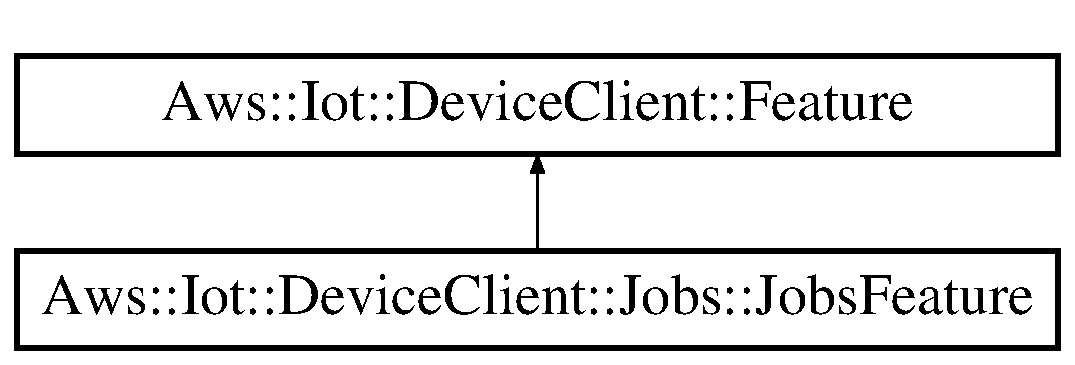
\includegraphics[height=2.000000cm]{class_aws_1_1_iot_1_1_device_client_1_1_jobs_1_1_jobs_feature}
\end{center}
\end{figure}
\doxysubsection*{Classes}
\begin{DoxyCompactItemize}
\item 
struct \mbox{\hyperlink{struct_aws_1_1_iot_1_1_device_client_1_1_jobs_1_1_jobs_feature_1_1_job_execution_status_info}{Job\+Execution\+Status\+Info}}
\begin{DoxyCompactList}\small\item\em Wrapper struct to aggregate \mbox{\hyperlink{class_aws_1_1_iot_1_1_device_client_1_1_jobs_1_1_job_engine}{Job\+Engine}} output for updating a job execution status. \end{DoxyCompactList}\end{DoxyCompactItemize}
\doxysubsection*{Public Member Functions}
\begin{DoxyCompactItemize}
\item 
virtual std\+::string \mbox{\hyperlink{class_aws_1_1_iot_1_1_device_client_1_1_jobs_1_1_jobs_feature_a88bff915e713b132ce5a49a3d60ba294}{get\+Name}} ()
\begin{DoxyCompactList}\small\item\em For a given feature, returns its name. \end{DoxyCompactList}\item 
virtual int \mbox{\hyperlink{class_aws_1_1_iot_1_1_device_client_1_1_jobs_1_1_jobs_feature_ae5ed8ac46280309eb3918b1d19ec1c54}{init}} (std\+::shared\+\_\+ptr$<$ \mbox{\hyperlink{class_aws_1_1_iot_1_1_device_client_1_1_shared_crt_resource_manager}{Shared\+Crt\+Resource\+Manager}} $>$ manager, std\+::shared\+\_\+ptr$<$ \mbox{\hyperlink{class_aws_1_1_iot_1_1_device_client_1_1_client_base_notifier}{Client\+Base\+Notifier}} $>$ notifier, const \mbox{\hyperlink{struct_aws_1_1_iot_1_1_device_client_1_1_plain_config}{Plain\+Config}} \&config)
\begin{DoxyCompactList}\small\item\em Initializes the Jobs feature with all the required setup information, event handlers, and the shared Mqtt\+Connection. \end{DoxyCompactList}\item 
virtual int \mbox{\hyperlink{class_aws_1_1_iot_1_1_device_client_1_1_jobs_1_1_jobs_feature_a6369b1914ce964ca98c9474a38e3214f}{start}} ()
\begin{DoxyCompactList}\small\item\em Start the feature. \end{DoxyCompactList}\item 
virtual int \mbox{\hyperlink{class_aws_1_1_iot_1_1_device_client_1_1_jobs_1_1_jobs_feature_aeec6332d60872b2a4471f6494f93b1c4}{stop}} ()
\begin{DoxyCompactList}\small\item\em Stop the feature. \end{DoxyCompactList}\end{DoxyCompactItemize}
\doxysubsection*{Private Member Functions}
\begin{DoxyCompactItemize}
\item 
void \mbox{\hyperlink{class_aws_1_1_iot_1_1_device_client_1_1_jobs_1_1_jobs_feature_a4031ad851a1bb42ced1392fb32090e46}{ack\+Subscribe\+To\+Next\+Job\+Changed}} (int io\+Error)
\begin{DoxyCompactList}\small\item\em Acknowledgement that IoT Core has received our request for subscription to Next\+Job\+Changed. \end{DoxyCompactList}\item 
void \mbox{\hyperlink{class_aws_1_1_iot_1_1_device_client_1_1_jobs_1_1_jobs_feature_a61eaca0e8195d1805b1ea94b39d04474}{ack\+Subscribe\+To\+Start\+Next\+Job\+Accepted}} (int io\+Error)
\begin{DoxyCompactList}\small\item\em Acknowledgement that IoT Core has received our request for subscription to Start\+Next\+Job\+Accepted. \end{DoxyCompactList}\item 
void \mbox{\hyperlink{class_aws_1_1_iot_1_1_device_client_1_1_jobs_1_1_jobs_feature_ae34fa1e7a48d09d81b7007c991a1719f}{ack\+Subscribe\+To\+Start\+Next\+Job\+Rejected}} (int io\+Error)
\begin{DoxyCompactList}\small\item\em Acknowledgement that IoT Core has received our request for subscription to Start\+Next\+Job\+Rejected. \end{DoxyCompactList}\item 
void \mbox{\hyperlink{class_aws_1_1_iot_1_1_device_client_1_1_jobs_1_1_jobs_feature_a63306a1777aae7bb64a3e80bc1285d72}{ack\+Start\+Next\+Pending\+Job\+Pub}} (int io\+Error)
\begin{DoxyCompactList}\small\item\em Acknowledgement that IoT Core has received our Start\+Next\+Pending\+Job message. \end{DoxyCompactList}\item 
void \mbox{\hyperlink{class_aws_1_1_iot_1_1_device_client_1_1_jobs_1_1_jobs_feature_abfca3cadf2210cea1b6fcc82bbb21725}{ack\+Update\+Job\+Execution\+Status}} (int io\+Error)
\begin{DoxyCompactList}\small\item\em Acknowledgement that IoT Core has received our Update\+Job\+Execution\+Status message. \end{DoxyCompactList}\item 
\mbox{\Hypertarget{class_aws_1_1_iot_1_1_device_client_1_1_jobs_1_1_jobs_feature_a881265a4086c4c66345d34f563f12280}\label{class_aws_1_1_iot_1_1_device_client_1_1_jobs_1_1_jobs_feature_a881265a4086c4c66345d34f563f12280}} 
void {\bfseries ack\+Subscribe\+To\+Update\+Job\+Execution\+Accepted} (int io\+Error)
\item 
\mbox{\Hypertarget{class_aws_1_1_iot_1_1_device_client_1_1_jobs_1_1_jobs_feature_aad6b16ad9e5bffe134be6ba660ad5fea}\label{class_aws_1_1_iot_1_1_device_client_1_1_jobs_1_1_jobs_feature_aad6b16ad9e5bffe134be6ba660ad5fea}} 
void {\bfseries ack\+Subscribe\+To\+Update\+Job\+Execution\+Rejected} (int io\+Error)
\item 
void \mbox{\hyperlink{class_aws_1_1_iot_1_1_device_client_1_1_jobs_1_1_jobs_feature_a546393fde6216c790c95d6a7a6903ddc}{publish\+Start\+Next\+Pending\+Job\+Execution\+Request}} ()
\begin{DoxyCompactList}\small\item\em Publishes a request to start\+Next\+Pending\+Job\+Execution. \end{DoxyCompactList}\item 
void \mbox{\hyperlink{class_aws_1_1_iot_1_1_device_client_1_1_jobs_1_1_jobs_feature_af56753139f5926916926fc15d1b43f58}{publish\+Update\+Job\+Execution\+Status}} (Aws\+::\+Iotjobs\+::\+Job\+Execution\+Data data, \mbox{\hyperlink{struct_aws_1_1_iot_1_1_device_client_1_1_jobs_1_1_jobs_feature_1_1_job_execution_status_info}{Job\+Execution\+Status\+Info}} status\+Info)
\begin{DoxyCompactList}\small\item\em Attempts to update a job execution to the provided status. \end{DoxyCompactList}\item 
void \mbox{\hyperlink{class_aws_1_1_iot_1_1_device_client_1_1_jobs_1_1_jobs_feature_ab76653347635a003fda9e3748ee8d053}{subscribe\+To\+Start\+Next\+Pending\+Job\+Execution}} ()
\begin{DoxyCompactList}\small\item\em Creates a subscription to the start\+Next\+Pending\+Job\+Execution topic. \end{DoxyCompactList}\item 
void \mbox{\hyperlink{class_aws_1_1_iot_1_1_device_client_1_1_jobs_1_1_jobs_feature_a38337467d49ff8804886cb4cd5aa61d0}{subscribe\+To\+Next\+Job\+Changed\+Events}} ()
\begin{DoxyCompactList}\small\item\em Creates a subscription to Next\+Job\+Changed\+Events. \end{DoxyCompactList}\item 
void \mbox{\hyperlink{class_aws_1_1_iot_1_1_device_client_1_1_jobs_1_1_jobs_feature_a15e9508e5eac303329646830223ce927}{subscribe\+To\+Update\+Job\+Execution\+Status\+Accepted}} (std\+::string job\+Id)
\begin{DoxyCompactList}\small\item\em Enables the Jobs feature to receive response information from the IoT Jobs service when an update is accepted. \end{DoxyCompactList}\item 
void \mbox{\hyperlink{class_aws_1_1_iot_1_1_device_client_1_1_jobs_1_1_jobs_feature_a2769b90aae519400c54300cca7d0719c}{subscribe\+To\+Update\+Job\+Execution\+Status\+Rejected}} (std\+::string job\+Id)
\begin{DoxyCompactList}\small\item\em Enables the Jobs feature to receive response information from the IoT Jobs service when an update is rejected. \end{DoxyCompactList}\item 
void \mbox{\hyperlink{class_aws_1_1_iot_1_1_device_client_1_1_jobs_1_1_jobs_feature_a4a976be8e597b38a1eeaaadc6d048739}{start\+Next\+Pending\+Job\+Received\+Handler}} (Iotjobs\+::\+Start\+Next\+Job\+Execution\+Response $\ast$response, int io\+Error)
\begin{DoxyCompactList}\small\item\em Executed upon receiving a response to our request to Start\+Next\+Pending\+Job. \end{DoxyCompactList}\item 
void \mbox{\hyperlink{class_aws_1_1_iot_1_1_device_client_1_1_jobs_1_1_jobs_feature_a974eb6561346d4612c975a9df28ad516}{start\+Next\+Pending\+Job\+Rejected\+Handler}} (Iotjobs\+::\+Rejected\+Error $\ast$rejected\+Error, int io\+Error)
\begin{DoxyCompactList}\small\item\em Executed if our request to Start\+Next\+Pending\+Job is rejected. \end{DoxyCompactList}\item 
void \mbox{\hyperlink{class_aws_1_1_iot_1_1_device_client_1_1_jobs_1_1_jobs_feature_a699398d2cdb6ad04950408f957d57cf0}{next\+Job\+Changed\+Handler}} (Iotjobs\+::\+Next\+Job\+Execution\+Changed\+Event $\ast$event, int io\+Err)
\begin{DoxyCompactList}\small\item\em Executed when the next job for this thing to execute has changed. \end{DoxyCompactList}\item 
void \mbox{\hyperlink{class_aws_1_1_iot_1_1_device_client_1_1_jobs_1_1_jobs_feature_a5c763db4b185acc3beb7f292cab09f77}{update\+Job\+Execution\+Status\+Accepted\+Handler}} (Iotjobs\+::\+Update\+Job\+Execution\+Response $\ast$response, int io\+Error)
\item 
void \mbox{\hyperlink{class_aws_1_1_iot_1_1_device_client_1_1_jobs_1_1_jobs_feature_a15ac84770cecf46cd377c2f16d5994fa}{update\+Job\+Execution\+Status\+Rejected\+Handler}} (Iotjobs\+::\+Rejected\+Error $\ast$rejected\+Error, int io\+Error)
\item 
void \mbox{\hyperlink{class_aws_1_1_iot_1_1_device_client_1_1_jobs_1_1_jobs_feature_a021bbb91acaf6ef46ef41fb55ebff69e}{execute\+Job}} (Iotjobs\+::\+Job\+Execution\+Data job)
\begin{DoxyCompactList}\small\item\em Called to begin the execution of a job on the device. \end{DoxyCompactList}\item 
bool \mbox{\hyperlink{class_aws_1_1_iot_1_1_device_client_1_1_jobs_1_1_jobs_feature_a43ec792550c419ef608352d276f415c8}{is\+Duplicate\+Notification}} (Iotjobs\+::\+Job\+Execution\+Data job)
\begin{DoxyCompactList}\small\item\em Given a job notification, determines whether it\textquotesingle{}s a duplicate message. \end{DoxyCompactList}\item 
void \mbox{\hyperlink{class_aws_1_1_iot_1_1_device_client_1_1_jobs_1_1_jobs_feature_a9f121d4d293369a876b300d899f5867b}{copy\+Jobs\+Notification}} (Iotjobs\+::\+Job\+Execution\+Data job)
\begin{DoxyCompactList}\small\item\em Stores information about a job notification. \end{DoxyCompactList}\item 
\mbox{\Hypertarget{class_aws_1_1_iot_1_1_device_client_1_1_jobs_1_1_jobs_feature_ae42ed26b1a4bb83fe4f408f45729246f}\label{class_aws_1_1_iot_1_1_device_client_1_1_jobs_1_1_jobs_feature_ae42ed26b1a4bb83fe4f408f45729246f}} 
void \mbox{\hyperlink{class_aws_1_1_iot_1_1_device_client_1_1_jobs_1_1_jobs_feature_ae42ed26b1a4bb83fe4f408f45729246f}{run\+Jobs}} ()
\begin{DoxyCompactList}\small\item\em Begins running the Jobs feature. \end{DoxyCompactList}\end{DoxyCompactItemize}
\doxysubsection*{Private Attributes}
\begin{DoxyCompactItemize}
\item 
\mbox{\Hypertarget{class_aws_1_1_iot_1_1_device_client_1_1_jobs_1_1_jobs_feature_ac6fcbba9b37a075c82a8be74e0ef5941}\label{class_aws_1_1_iot_1_1_device_client_1_1_jobs_1_1_jobs_feature_ac6fcbba9b37a075c82a8be74e0ef5941}} 
const char $\ast$ \mbox{\hyperlink{class_aws_1_1_iot_1_1_device_client_1_1_jobs_1_1_jobs_feature_ac6fcbba9b37a075c82a8be74e0ef5941}{T\+AG}} = \char`\"{}Jobs\+Feature.\+cpp\char`\"{}
\begin{DoxyCompactList}\small\item\em Used by the logger to specify that log messages are coming from the Jobs feature. \end{DoxyCompactList}\item 
\mbox{\Hypertarget{class_aws_1_1_iot_1_1_device_client_1_1_jobs_1_1_jobs_feature_abc5ede80a369d78034b4a3b7e1700d09}\label{class_aws_1_1_iot_1_1_device_client_1_1_jobs_1_1_jobs_feature_abc5ede80a369d78034b4a3b7e1700d09}} 
const char $\ast$ \mbox{\hyperlink{class_aws_1_1_iot_1_1_device_client_1_1_jobs_1_1_jobs_feature_abc5ede80a369d78034b4a3b7e1700d09}{J\+O\+B\+\_\+\+A\+T\+T\+R\+\_\+\+OP}} = \char`\"{}operation\char`\"{}
\begin{DoxyCompactList}\small\item\em A field within a Job document that the Jobs feature uses to determine which job to run. \end{DoxyCompactList}\item 
\mbox{\Hypertarget{class_aws_1_1_iot_1_1_device_client_1_1_jobs_1_1_jobs_feature_ab4c8f275b27255bea9f67c2301ec1dfd}\label{class_aws_1_1_iot_1_1_device_client_1_1_jobs_1_1_jobs_feature_ab4c8f275b27255bea9f67c2301ec1dfd}} 
const char $\ast$ \mbox{\hyperlink{class_aws_1_1_iot_1_1_device_client_1_1_jobs_1_1_jobs_feature_ab4c8f275b27255bea9f67c2301ec1dfd}{J\+O\+B\+\_\+\+A\+T\+T\+R\+\_\+\+A\+R\+GS}} = \char`\"{}args\char`\"{}
\begin{DoxyCompactList}\small\item\em A field within a Job document that the Jobs feature uses to determine which arguments to pass to the operation being run. \end{DoxyCompactList}\item 
\mbox{\Hypertarget{class_aws_1_1_iot_1_1_device_client_1_1_jobs_1_1_jobs_feature_afd50429795fa66c3986132ca98f3d209}\label{class_aws_1_1_iot_1_1_device_client_1_1_jobs_1_1_jobs_feature_afd50429795fa66c3986132ca98f3d209}} 
const char $\ast$ \mbox{\hyperlink{class_aws_1_1_iot_1_1_device_client_1_1_jobs_1_1_jobs_feature_afd50429795fa66c3986132ca98f3d209}{J\+O\+B\+\_\+\+A\+T\+T\+R\+\_\+\+A\+L\+L\+O\+W\+\_\+\+S\+T\+D\+E\+RR}} = \char`\"{}allow\+Std\+Err\char`\"{}
\begin{DoxyCompactList}\small\item\em A field within a Job document that the Jobs feature uses to determine whether S\+T\+D\+E\+RR output issued by the child process should be marked as a job failure in IoT Core. \end{DoxyCompactList}\item 
\mbox{\Hypertarget{class_aws_1_1_iot_1_1_device_client_1_1_jobs_1_1_jobs_feature_af3faf0824c3b40e078452642ae53ff0e}\label{class_aws_1_1_iot_1_1_device_client_1_1_jobs_1_1_jobs_feature_af3faf0824c3b40e078452642ae53ff0e}} 
const char $\ast$ \mbox{\hyperlink{class_aws_1_1_iot_1_1_device_client_1_1_jobs_1_1_jobs_feature_af3faf0824c3b40e078452642ae53ff0e}{J\+O\+B\+\_\+\+A\+T\+T\+R\+\_\+\+I\+N\+C\+L\+U\+D\+E\+\_\+\+S\+T\+D\+O\+UT}} = \char`\"{}include\+Std\+Out\char`\"{}
\begin{DoxyCompactList}\small\item\em A field within a job document that the Jobs feature uses to determine whether S\+T\+D\+O\+UT issued by the child process should be published when updating the job execution status. \end{DoxyCompactList}\item 
const char $\ast$ \mbox{\hyperlink{class_aws_1_1_iot_1_1_device_client_1_1_jobs_1_1_jobs_feature_a7cb8aaf7a89223ff69bfa6752f35d7b3}{J\+O\+B\+\_\+\+A\+T\+T\+R\+\_\+\+P\+A\+TH}} = \char`\"{}path\char`\"{}
\begin{DoxyCompactList}\small\item\em A field within a Job document that the Jobs feature uses to determine the location of the executable that should be run to handle this job. \end{DoxyCompactList}\item 
\mbox{\Hypertarget{class_aws_1_1_iot_1_1_device_client_1_1_jobs_1_1_jobs_feature_ac840150bd4fe9cfe959ce742a15c2b15}\label{class_aws_1_1_iot_1_1_device_client_1_1_jobs_1_1_jobs_feature_ac840150bd4fe9cfe959ce742a15c2b15}} 
const char $\ast$ \mbox{\hyperlink{class_aws_1_1_iot_1_1_device_client_1_1_jobs_1_1_jobs_feature_ac840150bd4fe9cfe959ce742a15c2b15}{D\+E\+F\+A\+U\+L\+T\+\_\+\+P\+A\+T\+H\+\_\+\+K\+E\+Y\+W\+O\+RD}} = \char`\"{}default\char`\"{}
\begin{DoxyCompactList}\small\item\em A keyword that can be specified as the \char`\"{}path\char`\"{} in a job doc to tell the Jobs feature to use the configured handler directory when looking for an executable matching the specified operation. \end{DoxyCompactList}\item 
const size\+\_\+t \mbox{\hyperlink{class_aws_1_1_iot_1_1_device_client_1_1_jobs_1_1_jobs_feature_a3f0629514f8a97930ded3e64aae5f952}{M\+A\+X\+\_\+\+S\+T\+A\+T\+U\+S\+\_\+\+D\+E\+T\+A\+I\+L\+\_\+\+L\+E\+N\+G\+TH}} = 1024
\begin{DoxyCompactList}\small\item\em The default directory that the Jobs feature will use to find executables matching an incoming job document\textquotesingle{}s operation attribute. \end{DoxyCompactList}\item 
\mbox{\Hypertarget{class_aws_1_1_iot_1_1_device_client_1_1_jobs_1_1_jobs_feature_a2a626ee75dcbf527b70ea572b2bcfa82}\label{class_aws_1_1_iot_1_1_device_client_1_1_jobs_1_1_jobs_feature_a2a626ee75dcbf527b70ea572b2bcfa82}} 
const int {\bfseries U\+P\+D\+A\+T\+E\+\_\+\+J\+O\+B\+\_\+\+E\+X\+E\+C\+U\+T\+I\+O\+N\+\_\+\+R\+E\+J\+E\+C\+T\+E\+D\+\_\+\+C\+O\+DE} = -\/1
\item 
\mbox{\Hypertarget{class_aws_1_1_iot_1_1_device_client_1_1_jobs_1_1_jobs_feature_a22e3bd36ee066ec60907ddb725a6c643}\label{class_aws_1_1_iot_1_1_device_client_1_1_jobs_1_1_jobs_feature_a22e3bd36ee066ec60907ddb725a6c643}} 
const std\+::string {\bfseries D\+E\+F\+A\+U\+L\+T\+\_\+\+J\+O\+B\+S\+\_\+\+H\+A\+N\+D\+L\+E\+R\+\_\+\+D\+IR} = \char`\"{}$\sim$/.aws-\/iot-\/device-\/client/jobs/\char`\"{}
\item 
\mbox{\Hypertarget{class_aws_1_1_iot_1_1_device_client_1_1_jobs_1_1_jobs_feature_accbc5327b89ebfb18643bf9f6fd9d04c}\label{class_aws_1_1_iot_1_1_device_client_1_1_jobs_1_1_jobs_feature_accbc5327b89ebfb18643bf9f6fd9d04c}} 
bool \mbox{\hyperlink{class_aws_1_1_iot_1_1_device_client_1_1_jobs_1_1_jobs_feature_accbc5327b89ebfb18643bf9f6fd9d04c}{need\+Stop}} = false
\begin{DoxyCompactList}\small\item\em Whether the Device\+Client base has requested this feature to stop. \end{DoxyCompactList}\item 
\mbox{\Hypertarget{class_aws_1_1_iot_1_1_device_client_1_1_jobs_1_1_jobs_feature_a2e4e736a9fb9a2ade61c0aad2c1e3ff6}\label{class_aws_1_1_iot_1_1_device_client_1_1_jobs_1_1_jobs_feature_a2e4e736a9fb9a2ade61c0aad2c1e3ff6}} 
bool \mbox{\hyperlink{class_aws_1_1_iot_1_1_device_client_1_1_jobs_1_1_jobs_feature_a2e4e736a9fb9a2ade61c0aad2c1e3ff6}{handling\+Job}} = false
\begin{DoxyCompactList}\small\item\em Whether the jobs feature is currently executing a job. \end{DoxyCompactList}\item 
\mbox{\Hypertarget{class_aws_1_1_iot_1_1_device_client_1_1_jobs_1_1_jobs_feature_ae6a85898893eeec33ca229846157a500}\label{class_aws_1_1_iot_1_1_device_client_1_1_jobs_1_1_jobs_feature_ae6a85898893eeec33ca229846157a500}} 
std\+::mutex \mbox{\hyperlink{class_aws_1_1_iot_1_1_device_client_1_1_jobs_1_1_jobs_feature_ae6a85898893eeec33ca229846157a500}{can\+Stop\+Lock}}
\begin{DoxyCompactList}\small\item\em A mutex used to control access to the stop and handling job flags. \end{DoxyCompactList}\item 
\mbox{\Hypertarget{class_aws_1_1_iot_1_1_device_client_1_1_jobs_1_1_jobs_feature_ab4449de08e2cc376ff0c6942f56f15db}\label{class_aws_1_1_iot_1_1_device_client_1_1_jobs_1_1_jobs_feature_ab4449de08e2cc376ff0c6942f56f15db}} 
std\+::mutex \mbox{\hyperlink{class_aws_1_1_iot_1_1_device_client_1_1_jobs_1_1_jobs_feature_ab4449de08e2cc376ff0c6942f56f15db}{update\+Job\+Execution\+Promises\+Lock}}
\begin{DoxyCompactList}\small\item\em A lock used to control access to the map of \mbox{\hyperlink{class_aws_1_1_iot_1_1_device_client_1_1_jobs_1_1_ephemeral_promise}{Ephemeral\+Promise}}. \end{DoxyCompactList}\item 
\mbox{\Hypertarget{class_aws_1_1_iot_1_1_device_client_1_1_jobs_1_1_jobs_feature_afb82743d214fa7dce63125b5809fd97e}\label{class_aws_1_1_iot_1_1_device_client_1_1_jobs_1_1_jobs_feature_afb82743d214fa7dce63125b5809fd97e}} 
Aws\+::\+Crt\+::\+Map$<$ Aws\+::\+Crt\+::\+String, \mbox{\hyperlink{class_aws_1_1_iot_1_1_device_client_1_1_jobs_1_1_ephemeral_promise}{Aws\+::\+Iot\+::\+Device\+Client\+::\+Jobs\+::\+Ephemeral\+Promise}}$<$ int $>$ $>$ \mbox{\hyperlink{class_aws_1_1_iot_1_1_device_client_1_1_jobs_1_1_jobs_feature_afb82743d214fa7dce63125b5809fd97e}{update\+Job\+Execution\+Promises}}
\begin{DoxyCompactList}\small\item\em Allows us to map Update\+Job\+Execution responses back to their original request. \end{DoxyCompactList}\item 
\mbox{\Hypertarget{class_aws_1_1_iot_1_1_device_client_1_1_jobs_1_1_jobs_feature_ac836a3bd8d835654076ea56bc7a57745}\label{class_aws_1_1_iot_1_1_device_client_1_1_jobs_1_1_jobs_feature_ac836a3bd8d835654076ea56bc7a57745}} 
std\+::mutex {\bfseries latest\+Jobs\+Notification\+Lock}
\item 
\mbox{\Hypertarget{class_aws_1_1_iot_1_1_device_client_1_1_jobs_1_1_jobs_feature_a96f7c2f34ed5fefb690f51fbc94f00e5}\label{class_aws_1_1_iot_1_1_device_client_1_1_jobs_1_1_jobs_feature_a96f7c2f34ed5fefb690f51fbc94f00e5}} 
Aws\+::\+Iotjobs\+::\+Job\+Execution\+Data {\bfseries latest\+Jobs\+Notification}
\item 
\mbox{\Hypertarget{class_aws_1_1_iot_1_1_device_client_1_1_jobs_1_1_jobs_feature_ab798b4c4f1f9790ff6b92002bf13533f}\label{class_aws_1_1_iot_1_1_device_client_1_1_jobs_1_1_jobs_feature_ab798b4c4f1f9790ff6b92002bf13533f}} 
std\+::shared\+\_\+ptr$<$ \mbox{\hyperlink{class_aws_1_1_iot_1_1_device_client_1_1_shared_crt_resource_manager}{Shared\+Crt\+Resource\+Manager}} $>$ \mbox{\hyperlink{class_aws_1_1_iot_1_1_device_client_1_1_jobs_1_1_jobs_feature_ab798b4c4f1f9790ff6b92002bf13533f}{resource\+Manager}}
\begin{DoxyCompactList}\small\item\em The resource manager used to manage C\+RT resources. \end{DoxyCompactList}\item 
\mbox{\Hypertarget{class_aws_1_1_iot_1_1_device_client_1_1_jobs_1_1_jobs_feature_a2f7ddca3946641f18591475b0072044d}\label{class_aws_1_1_iot_1_1_device_client_1_1_jobs_1_1_jobs_feature_a2f7ddca3946641f18591475b0072044d}} 
std\+::shared\+\_\+ptr$<$ \mbox{\hyperlink{class_aws_1_1_iot_1_1_device_client_1_1_client_base_notifier}{Client\+Base\+Notifier}} $>$ \mbox{\hyperlink{class_aws_1_1_iot_1_1_device_client_1_1_jobs_1_1_jobs_feature_a2f7ddca3946641f18591475b0072044d}{base\+Notifier}}
\begin{DoxyCompactList}\small\item\em An interface used to notify the Client base if there is an event that requires its attention. \end{DoxyCompactList}\item 
\mbox{\Hypertarget{class_aws_1_1_iot_1_1_device_client_1_1_jobs_1_1_jobs_feature_a3e1943f1c6c221953e2d6dd884adcb0d}\label{class_aws_1_1_iot_1_1_device_client_1_1_jobs_1_1_jobs_feature_a3e1943f1c6c221953e2d6dd884adcb0d}} 
std\+::unique\+\_\+ptr$<$ Aws\+::\+Iotjobs\+::\+Iot\+Jobs\+Client $>$ \mbox{\hyperlink{class_aws_1_1_iot_1_1_device_client_1_1_jobs_1_1_jobs_feature_a3e1943f1c6c221953e2d6dd884adcb0d}{jobs\+Client}}
\begin{DoxyCompactList}\small\item\em an Iot\+Jobs\+Client used to make calls to the A\+WS IoT Jobs service \end{DoxyCompactList}\item 
\mbox{\Hypertarget{class_aws_1_1_iot_1_1_device_client_1_1_jobs_1_1_jobs_feature_a10d7baa43855fc9d73404ddfc03eb347}\label{class_aws_1_1_iot_1_1_device_client_1_1_jobs_1_1_jobs_feature_a10d7baa43855fc9d73404ddfc03eb347}} 
std\+::string \mbox{\hyperlink{class_aws_1_1_iot_1_1_device_client_1_1_jobs_1_1_jobs_feature_a10d7baa43855fc9d73404ddfc03eb347}{thing\+Name}}
\begin{DoxyCompactList}\small\item\em the Thing\+Name to use \end{DoxyCompactList}\item 
\mbox{\Hypertarget{class_aws_1_1_iot_1_1_device_client_1_1_jobs_1_1_jobs_feature_a37030f5e63e8d42448dab3a0dd70d7b2}\label{class_aws_1_1_iot_1_1_device_client_1_1_jobs_1_1_jobs_feature_a37030f5e63e8d42448dab3a0dd70d7b2}} 
std\+::string \mbox{\hyperlink{class_aws_1_1_iot_1_1_device_client_1_1_jobs_1_1_jobs_feature_a37030f5e63e8d42448dab3a0dd70d7b2}{job\+Handler\+Dir}} = D\+E\+F\+A\+U\+L\+T\+\_\+\+J\+O\+B\+S\+\_\+\+H\+A\+N\+D\+L\+E\+R\+\_\+\+D\+IR
\begin{DoxyCompactList}\small\item\em User provided handler directory passed either through command-\/line arguments or through the Json configuration file. \end{DoxyCompactList}\end{DoxyCompactItemize}


\doxysubsection{Detailed Description}
Provides IoT Jobs related functionality within the Device Client. 

\doxysubsection{Member Function Documentation}
\mbox{\Hypertarget{class_aws_1_1_iot_1_1_device_client_1_1_jobs_1_1_jobs_feature_a63306a1777aae7bb64a3e80bc1285d72}\label{class_aws_1_1_iot_1_1_device_client_1_1_jobs_1_1_jobs_feature_a63306a1777aae7bb64a3e80bc1285d72}} 
\index{Aws::Iot::DeviceClient::Jobs::JobsFeature@{Aws::Iot::DeviceClient::Jobs::JobsFeature}!ackStartNextPendingJobPub@{ackStartNextPendingJobPub}}
\index{ackStartNextPendingJobPub@{ackStartNextPendingJobPub}!Aws::Iot::DeviceClient::Jobs::JobsFeature@{Aws::Iot::DeviceClient::Jobs::JobsFeature}}
\doxysubsubsection{\texorpdfstring{ackStartNextPendingJobPub()}{ackStartNextPendingJobPub()}}
{\footnotesize\ttfamily void Jobs\+Feature\+::ack\+Start\+Next\+Pending\+Job\+Pub (\begin{DoxyParamCaption}\item[{int}]{io\+Error }\end{DoxyParamCaption})\hspace{0.3cm}{\ttfamily [private]}}



Acknowledgement that IoT Core has received our Start\+Next\+Pending\+Job message. 


\begin{DoxyParams}{Parameters}
{\em io\+Error} & a non-\/zero code here indicates a problem. Turn on logging in IoT Core and check Cloud\+Watch for more insights on errors \\
\hline
\end{DoxyParams}
\mbox{\Hypertarget{class_aws_1_1_iot_1_1_device_client_1_1_jobs_1_1_jobs_feature_a4031ad851a1bb42ced1392fb32090e46}\label{class_aws_1_1_iot_1_1_device_client_1_1_jobs_1_1_jobs_feature_a4031ad851a1bb42ced1392fb32090e46}} 
\index{Aws::Iot::DeviceClient::Jobs::JobsFeature@{Aws::Iot::DeviceClient::Jobs::JobsFeature}!ackSubscribeToNextJobChanged@{ackSubscribeToNextJobChanged}}
\index{ackSubscribeToNextJobChanged@{ackSubscribeToNextJobChanged}!Aws::Iot::DeviceClient::Jobs::JobsFeature@{Aws::Iot::DeviceClient::Jobs::JobsFeature}}
\doxysubsubsection{\texorpdfstring{ackSubscribeToNextJobChanged()}{ackSubscribeToNextJobChanged()}}
{\footnotesize\ttfamily void Jobs\+Feature\+::ack\+Subscribe\+To\+Next\+Job\+Changed (\begin{DoxyParamCaption}\item[{int}]{io\+Error }\end{DoxyParamCaption})\hspace{0.3cm}{\ttfamily [private]}}



Acknowledgement that IoT Core has received our request for subscription to Next\+Job\+Changed. 


\begin{DoxyParams}{Parameters}
{\em io\+Error} & a non-\/zero code here indicates a problem. Turn on logging in IoT Core and check Cloud\+Watch for more insights on errors \\
\hline
\end{DoxyParams}
\mbox{\Hypertarget{class_aws_1_1_iot_1_1_device_client_1_1_jobs_1_1_jobs_feature_a61eaca0e8195d1805b1ea94b39d04474}\label{class_aws_1_1_iot_1_1_device_client_1_1_jobs_1_1_jobs_feature_a61eaca0e8195d1805b1ea94b39d04474}} 
\index{Aws::Iot::DeviceClient::Jobs::JobsFeature@{Aws::Iot::DeviceClient::Jobs::JobsFeature}!ackSubscribeToStartNextJobAccepted@{ackSubscribeToStartNextJobAccepted}}
\index{ackSubscribeToStartNextJobAccepted@{ackSubscribeToStartNextJobAccepted}!Aws::Iot::DeviceClient::Jobs::JobsFeature@{Aws::Iot::DeviceClient::Jobs::JobsFeature}}
\doxysubsubsection{\texorpdfstring{ackSubscribeToStartNextJobAccepted()}{ackSubscribeToStartNextJobAccepted()}}
{\footnotesize\ttfamily void Jobs\+Feature\+::ack\+Subscribe\+To\+Start\+Next\+Job\+Accepted (\begin{DoxyParamCaption}\item[{int}]{io\+Error }\end{DoxyParamCaption})\hspace{0.3cm}{\ttfamily [private]}}



Acknowledgement that IoT Core has received our request for subscription to Start\+Next\+Job\+Accepted. 


\begin{DoxyParams}{Parameters}
{\em io\+Error} & a non-\/zero code here indicates a problem. Turn on logging in IoT Core and check Cloud\+Watch for more insights on errors \\
\hline
\end{DoxyParams}
\mbox{\Hypertarget{class_aws_1_1_iot_1_1_device_client_1_1_jobs_1_1_jobs_feature_ae34fa1e7a48d09d81b7007c991a1719f}\label{class_aws_1_1_iot_1_1_device_client_1_1_jobs_1_1_jobs_feature_ae34fa1e7a48d09d81b7007c991a1719f}} 
\index{Aws::Iot::DeviceClient::Jobs::JobsFeature@{Aws::Iot::DeviceClient::Jobs::JobsFeature}!ackSubscribeToStartNextJobRejected@{ackSubscribeToStartNextJobRejected}}
\index{ackSubscribeToStartNextJobRejected@{ackSubscribeToStartNextJobRejected}!Aws::Iot::DeviceClient::Jobs::JobsFeature@{Aws::Iot::DeviceClient::Jobs::JobsFeature}}
\doxysubsubsection{\texorpdfstring{ackSubscribeToStartNextJobRejected()}{ackSubscribeToStartNextJobRejected()}}
{\footnotesize\ttfamily void Jobs\+Feature\+::ack\+Subscribe\+To\+Start\+Next\+Job\+Rejected (\begin{DoxyParamCaption}\item[{int}]{io\+Error }\end{DoxyParamCaption})\hspace{0.3cm}{\ttfamily [private]}}



Acknowledgement that IoT Core has received our request for subscription to Start\+Next\+Job\+Rejected. 


\begin{DoxyParams}{Parameters}
{\em io\+Error} & a non-\/zero code here indicates a problem. Turn on logging in IoT Core and check Cloud\+Watch for more insights on errors \\
\hline
\end{DoxyParams}
\mbox{\Hypertarget{class_aws_1_1_iot_1_1_device_client_1_1_jobs_1_1_jobs_feature_abfca3cadf2210cea1b6fcc82bbb21725}\label{class_aws_1_1_iot_1_1_device_client_1_1_jobs_1_1_jobs_feature_abfca3cadf2210cea1b6fcc82bbb21725}} 
\index{Aws::Iot::DeviceClient::Jobs::JobsFeature@{Aws::Iot::DeviceClient::Jobs::JobsFeature}!ackUpdateJobExecutionStatus@{ackUpdateJobExecutionStatus}}
\index{ackUpdateJobExecutionStatus@{ackUpdateJobExecutionStatus}!Aws::Iot::DeviceClient::Jobs::JobsFeature@{Aws::Iot::DeviceClient::Jobs::JobsFeature}}
\doxysubsubsection{\texorpdfstring{ackUpdateJobExecutionStatus()}{ackUpdateJobExecutionStatus()}}
{\footnotesize\ttfamily void Jobs\+Feature\+::ack\+Update\+Job\+Execution\+Status (\begin{DoxyParamCaption}\item[{int}]{io\+Error }\end{DoxyParamCaption})\hspace{0.3cm}{\ttfamily [private]}}



Acknowledgement that IoT Core has received our Update\+Job\+Execution\+Status message. 


\begin{DoxyParams}{Parameters}
{\em io\+Error} & a non-\/zero code here indicates a problem. Turn on logging in IoT Core and check Cloud\+Watch for more insights on errors \\
\hline
\end{DoxyParams}
\mbox{\Hypertarget{class_aws_1_1_iot_1_1_device_client_1_1_jobs_1_1_jobs_feature_a9f121d4d293369a876b300d899f5867b}\label{class_aws_1_1_iot_1_1_device_client_1_1_jobs_1_1_jobs_feature_a9f121d4d293369a876b300d899f5867b}} 
\index{Aws::Iot::DeviceClient::Jobs::JobsFeature@{Aws::Iot::DeviceClient::Jobs::JobsFeature}!copyJobsNotification@{copyJobsNotification}}
\index{copyJobsNotification@{copyJobsNotification}!Aws::Iot::DeviceClient::Jobs::JobsFeature@{Aws::Iot::DeviceClient::Jobs::JobsFeature}}
\doxysubsubsection{\texorpdfstring{copyJobsNotification()}{copyJobsNotification()}}
{\footnotesize\ttfamily void Jobs\+Feature\+::copy\+Jobs\+Notification (\begin{DoxyParamCaption}\item[{Iotjobs\+::\+Job\+Execution\+Data}]{job }\end{DoxyParamCaption})\hspace{0.3cm}{\ttfamily [private]}}



Stores information about a job notification. 


\begin{DoxyParams}{Parameters}
{\em job} & \\
\hline
\end{DoxyParams}
\mbox{\Hypertarget{class_aws_1_1_iot_1_1_device_client_1_1_jobs_1_1_jobs_feature_a021bbb91acaf6ef46ef41fb55ebff69e}\label{class_aws_1_1_iot_1_1_device_client_1_1_jobs_1_1_jobs_feature_a021bbb91acaf6ef46ef41fb55ebff69e}} 
\index{Aws::Iot::DeviceClient::Jobs::JobsFeature@{Aws::Iot::DeviceClient::Jobs::JobsFeature}!executeJob@{executeJob}}
\index{executeJob@{executeJob}!Aws::Iot::DeviceClient::Jobs::JobsFeature@{Aws::Iot::DeviceClient::Jobs::JobsFeature}}
\doxysubsubsection{\texorpdfstring{executeJob()}{executeJob()}}
{\footnotesize\ttfamily void Jobs\+Feature\+::execute\+Job (\begin{DoxyParamCaption}\item[{Iotjobs\+::\+Job\+Execution\+Data}]{job }\end{DoxyParamCaption})\hspace{0.3cm}{\ttfamily [private]}}



Called to begin the execution of a job on the device. 


\begin{DoxyParams}{Parameters}
{\em job} & the job to execute \\
\hline
\end{DoxyParams}
\mbox{\Hypertarget{class_aws_1_1_iot_1_1_device_client_1_1_jobs_1_1_jobs_feature_a88bff915e713b132ce5a49a3d60ba294}\label{class_aws_1_1_iot_1_1_device_client_1_1_jobs_1_1_jobs_feature_a88bff915e713b132ce5a49a3d60ba294}} 
\index{Aws::Iot::DeviceClient::Jobs::JobsFeature@{Aws::Iot::DeviceClient::Jobs::JobsFeature}!getName@{getName}}
\index{getName@{getName}!Aws::Iot::DeviceClient::Jobs::JobsFeature@{Aws::Iot::DeviceClient::Jobs::JobsFeature}}
\doxysubsubsection{\texorpdfstring{getName()}{getName()}}
{\footnotesize\ttfamily string Jobs\+Feature\+::get\+Name (\begin{DoxyParamCaption}{ }\end{DoxyParamCaption})\hspace{0.3cm}{\ttfamily [virtual]}}



For a given feature, returns its name. 

\begin{DoxyReturn}{Returns}
a string value representing the feature\textquotesingle{}s name 
\end{DoxyReturn}


Implements \mbox{\hyperlink{class_aws_1_1_iot_1_1_device_client_1_1_feature_a7f56b81457898d67ddc1942e57e3c0d5}{Aws\+::\+Iot\+::\+Device\+Client\+::\+Feature}}.

\mbox{\Hypertarget{class_aws_1_1_iot_1_1_device_client_1_1_jobs_1_1_jobs_feature_ae5ed8ac46280309eb3918b1d19ec1c54}\label{class_aws_1_1_iot_1_1_device_client_1_1_jobs_1_1_jobs_feature_ae5ed8ac46280309eb3918b1d19ec1c54}} 
\index{Aws::Iot::DeviceClient::Jobs::JobsFeature@{Aws::Iot::DeviceClient::Jobs::JobsFeature}!init@{init}}
\index{init@{init}!Aws::Iot::DeviceClient::Jobs::JobsFeature@{Aws::Iot::DeviceClient::Jobs::JobsFeature}}
\doxysubsubsection{\texorpdfstring{init()}{init()}}
{\footnotesize\ttfamily int Jobs\+Feature\+::init (\begin{DoxyParamCaption}\item[{std\+::shared\+\_\+ptr$<$ \mbox{\hyperlink{class_aws_1_1_iot_1_1_device_client_1_1_shared_crt_resource_manager}{Shared\+Crt\+Resource\+Manager}} $>$}]{manager,  }\item[{std\+::shared\+\_\+ptr$<$ \mbox{\hyperlink{class_aws_1_1_iot_1_1_device_client_1_1_client_base_notifier}{Client\+Base\+Notifier}} $>$}]{notifier,  }\item[{const \mbox{\hyperlink{struct_aws_1_1_iot_1_1_device_client_1_1_plain_config}{Plain\+Config}} \&}]{config }\end{DoxyParamCaption})\hspace{0.3cm}{\ttfamily [virtual]}}



Initializes the Jobs feature with all the required setup information, event handlers, and the shared Mqtt\+Connection. 


\begin{DoxyParams}{Parameters}
{\em manager} & the shared Mqtt\+Connection\+Manager \\
\hline
{\em notifier} & an \mbox{\hyperlink{class_aws_1_1_iot_1_1_device_client_1_1_client_base_notifier}{Client\+Base\+Notifier}} used for notifying the client base of events or errors \\
\hline
{\em config} & configuration information passed in by the user via either the command line or configuration file \\
\hline
\end{DoxyParams}
\begin{DoxyReturn}{Returns}
a non-\/zero return code indicates a problem. The logs can be checked for more info 
\end{DoxyReturn}
\mbox{\Hypertarget{class_aws_1_1_iot_1_1_device_client_1_1_jobs_1_1_jobs_feature_a43ec792550c419ef608352d276f415c8}\label{class_aws_1_1_iot_1_1_device_client_1_1_jobs_1_1_jobs_feature_a43ec792550c419ef608352d276f415c8}} 
\index{Aws::Iot::DeviceClient::Jobs::JobsFeature@{Aws::Iot::DeviceClient::Jobs::JobsFeature}!isDuplicateNotification@{isDuplicateNotification}}
\index{isDuplicateNotification@{isDuplicateNotification}!Aws::Iot::DeviceClient::Jobs::JobsFeature@{Aws::Iot::DeviceClient::Jobs::JobsFeature}}
\doxysubsubsection{\texorpdfstring{isDuplicateNotification()}{isDuplicateNotification()}}
{\footnotesize\ttfamily bool Jobs\+Feature\+::is\+Duplicate\+Notification (\begin{DoxyParamCaption}\item[{Iotjobs\+::\+Job\+Execution\+Data}]{job }\end{DoxyParamCaption})\hspace{0.3cm}{\ttfamily [private]}}



Given a job notification, determines whether it\textquotesingle{}s a duplicate message. 

This method was originally intended to handle scenarios such as network instability or loss where the jobs feature may receive multiple instances of the same message. This allows us to eliminate duplicates that would otherwise cause the Jobs feature to run the same job more than once. 
\begin{DoxyParams}{Parameters}
{\em job} & \\
\hline
\end{DoxyParams}
\begin{DoxyReturn}{Returns}
true if it\textquotesingle{}s a duplicate, false otherwise 
\end{DoxyReturn}
\mbox{\Hypertarget{class_aws_1_1_iot_1_1_device_client_1_1_jobs_1_1_jobs_feature_a699398d2cdb6ad04950408f957d57cf0}\label{class_aws_1_1_iot_1_1_device_client_1_1_jobs_1_1_jobs_feature_a699398d2cdb6ad04950408f957d57cf0}} 
\index{Aws::Iot::DeviceClient::Jobs::JobsFeature@{Aws::Iot::DeviceClient::Jobs::JobsFeature}!nextJobChangedHandler@{nextJobChangedHandler}}
\index{nextJobChangedHandler@{nextJobChangedHandler}!Aws::Iot::DeviceClient::Jobs::JobsFeature@{Aws::Iot::DeviceClient::Jobs::JobsFeature}}
\doxysubsubsection{\texorpdfstring{nextJobChangedHandler()}{nextJobChangedHandler()}}
{\footnotesize\ttfamily void Jobs\+Feature\+::next\+Job\+Changed\+Handler (\begin{DoxyParamCaption}\item[{Iotjobs\+::\+Next\+Job\+Execution\+Changed\+Event $\ast$}]{event,  }\item[{int}]{io\+Err }\end{DoxyParamCaption})\hspace{0.3cm}{\ttfamily [private]}}



Executed when the next job for this thing to execute has changed. 

This typically happens after updating a job execution and the Jobs A\+PI is notifying the Device Client that we have a new job to execute 
\begin{DoxyParams}{Parameters}
{\em event} & information about the next job \\
\hline
{\em io\+Err} & a non-\/zero error code indicates a problem \\
\hline
\end{DoxyParams}
\mbox{\Hypertarget{class_aws_1_1_iot_1_1_device_client_1_1_jobs_1_1_jobs_feature_a546393fde6216c790c95d6a7a6903ddc}\label{class_aws_1_1_iot_1_1_device_client_1_1_jobs_1_1_jobs_feature_a546393fde6216c790c95d6a7a6903ddc}} 
\index{Aws::Iot::DeviceClient::Jobs::JobsFeature@{Aws::Iot::DeviceClient::Jobs::JobsFeature}!publishStartNextPendingJobExecutionRequest@{publishStartNextPendingJobExecutionRequest}}
\index{publishStartNextPendingJobExecutionRequest@{publishStartNextPendingJobExecutionRequest}!Aws::Iot::DeviceClient::Jobs::JobsFeature@{Aws::Iot::DeviceClient::Jobs::JobsFeature}}
\doxysubsubsection{\texorpdfstring{publishStartNextPendingJobExecutionRequest()}{publishStartNextPendingJobExecutionRequest()}}
{\footnotesize\ttfamily void Jobs\+Feature\+::publish\+Start\+Next\+Pending\+Job\+Execution\+Request (\begin{DoxyParamCaption}{ }\end{DoxyParamCaption})\hspace{0.3cm}{\ttfamily [private]}}



Publishes a request to start\+Next\+Pending\+Job\+Execution. 

Publishes a request to start the next pending job. In order to receive the response message, subscribe\+To\+Get\+Pending\+Jobs() must have been called successfully before this. \mbox{\Hypertarget{class_aws_1_1_iot_1_1_device_client_1_1_jobs_1_1_jobs_feature_af56753139f5926916926fc15d1b43f58}\label{class_aws_1_1_iot_1_1_device_client_1_1_jobs_1_1_jobs_feature_af56753139f5926916926fc15d1b43f58}} 
\index{Aws::Iot::DeviceClient::Jobs::JobsFeature@{Aws::Iot::DeviceClient::Jobs::JobsFeature}!publishUpdateJobExecutionStatus@{publishUpdateJobExecutionStatus}}
\index{publishUpdateJobExecutionStatus@{publishUpdateJobExecutionStatus}!Aws::Iot::DeviceClient::Jobs::JobsFeature@{Aws::Iot::DeviceClient::Jobs::JobsFeature}}
\doxysubsubsection{\texorpdfstring{publishUpdateJobExecutionStatus()}{publishUpdateJobExecutionStatus()}}
{\footnotesize\ttfamily void Jobs\+Feature\+::publish\+Update\+Job\+Execution\+Status (\begin{DoxyParamCaption}\item[{Aws\+::\+Iotjobs\+::\+Job\+Execution\+Data}]{data,  }\item[{\mbox{\hyperlink{struct_aws_1_1_iot_1_1_device_client_1_1_jobs_1_1_jobs_feature_1_1_job_execution_status_info}{Job\+Execution\+Status\+Info}}}]{status\+Info }\end{DoxyParamCaption})\hspace{0.3cm}{\ttfamily [private]}}



Attempts to update a job execution to the provided status. 


\begin{DoxyParams}{Parameters}
{\em data} & Job\+Execution\+Data containing information about the job \\
\hline
{\em status\+Info} & status information including the Job status, as well as S\+T\+D\+O\+UT and S\+T\+D\+E\+RR from the child process \\
\hline
\end{DoxyParams}
When we update the job execution status, we need to perform an exponential backoff in case our request gets throttled. Otherwise, if we never properly update the job execution status, we\textquotesingle{}ll never receive the next job

no increment here\mbox{\Hypertarget{class_aws_1_1_iot_1_1_device_client_1_1_jobs_1_1_jobs_feature_a6369b1914ce964ca98c9474a38e3214f}\label{class_aws_1_1_iot_1_1_device_client_1_1_jobs_1_1_jobs_feature_a6369b1914ce964ca98c9474a38e3214f}} 
\index{Aws::Iot::DeviceClient::Jobs::JobsFeature@{Aws::Iot::DeviceClient::Jobs::JobsFeature}!start@{start}}
\index{start@{start}!Aws::Iot::DeviceClient::Jobs::JobsFeature@{Aws::Iot::DeviceClient::Jobs::JobsFeature}}
\doxysubsubsection{\texorpdfstring{start()}{start()}}
{\footnotesize\ttfamily int Jobs\+Feature\+::start (\begin{DoxyParamCaption}{ }\end{DoxyParamCaption})\hspace{0.3cm}{\ttfamily [virtual]}}



Start the feature. 

\begin{DoxyReturn}{Returns}
an integer representing the S\+U\+C\+C\+E\+SS or F\+A\+I\+L\+U\+RE of the \mbox{\hyperlink{class_aws_1_1_iot_1_1_device_client_1_1_jobs_1_1_jobs_feature_a6369b1914ce964ca98c9474a38e3214f}{start()}} operation on the feature 
\end{DoxyReturn}


Implements \mbox{\hyperlink{class_aws_1_1_iot_1_1_device_client_1_1_feature_ac9a936ebd88f7e35914a6aac99badf7d}{Aws\+::\+Iot\+::\+Device\+Client\+::\+Feature}}.

\mbox{\Hypertarget{class_aws_1_1_iot_1_1_device_client_1_1_jobs_1_1_jobs_feature_a4a976be8e597b38a1eeaaadc6d048739}\label{class_aws_1_1_iot_1_1_device_client_1_1_jobs_1_1_jobs_feature_a4a976be8e597b38a1eeaaadc6d048739}} 
\index{Aws::Iot::DeviceClient::Jobs::JobsFeature@{Aws::Iot::DeviceClient::Jobs::JobsFeature}!startNextPendingJobReceivedHandler@{startNextPendingJobReceivedHandler}}
\index{startNextPendingJobReceivedHandler@{startNextPendingJobReceivedHandler}!Aws::Iot::DeviceClient::Jobs::JobsFeature@{Aws::Iot::DeviceClient::Jobs::JobsFeature}}
\doxysubsubsection{\texorpdfstring{startNextPendingJobReceivedHandler()}{startNextPendingJobReceivedHandler()}}
{\footnotesize\ttfamily void Jobs\+Feature\+::start\+Next\+Pending\+Job\+Received\+Handler (\begin{DoxyParamCaption}\item[{Iotjobs\+::\+Start\+Next\+Job\+Execution\+Response $\ast$}]{response,  }\item[{int}]{io\+Error }\end{DoxyParamCaption})\hspace{0.3cm}{\ttfamily [private]}}



Executed upon receiving a response to our request to Start\+Next\+Pending\+Job. 


\begin{DoxyParams}{Parameters}
{\em response} & the response from Iot Core \\
\hline
{\em io\+Error} & a non-\/zero error code indicates a problem\\
\hline
\end{DoxyParams}
Upon receipt of the Pending\+Jobs message, this handler method will attempt to add the first available job to the Event\+Queue. \mbox{\Hypertarget{class_aws_1_1_iot_1_1_device_client_1_1_jobs_1_1_jobs_feature_a974eb6561346d4612c975a9df28ad516}\label{class_aws_1_1_iot_1_1_device_client_1_1_jobs_1_1_jobs_feature_a974eb6561346d4612c975a9df28ad516}} 
\index{Aws::Iot::DeviceClient::Jobs::JobsFeature@{Aws::Iot::DeviceClient::Jobs::JobsFeature}!startNextPendingJobRejectedHandler@{startNextPendingJobRejectedHandler}}
\index{startNextPendingJobRejectedHandler@{startNextPendingJobRejectedHandler}!Aws::Iot::DeviceClient::Jobs::JobsFeature@{Aws::Iot::DeviceClient::Jobs::JobsFeature}}
\doxysubsubsection{\texorpdfstring{startNextPendingJobRejectedHandler()}{startNextPendingJobRejectedHandler()}}
{\footnotesize\ttfamily void Jobs\+Feature\+::start\+Next\+Pending\+Job\+Rejected\+Handler (\begin{DoxyParamCaption}\item[{Iotjobs\+::\+Rejected\+Error $\ast$}]{rejected\+Error,  }\item[{int}]{io\+Error }\end{DoxyParamCaption})\hspace{0.3cm}{\ttfamily [private]}}



Executed if our request to Start\+Next\+Pending\+Job is rejected. 


\begin{DoxyParams}{Parameters}
{\em rejected\+Error} & information about the rejection \\
\hline
{\em io\+Error} & a non-\/zero error code indicates a problem \\
\hline
\end{DoxyParams}
\mbox{\Hypertarget{class_aws_1_1_iot_1_1_device_client_1_1_jobs_1_1_jobs_feature_aeec6332d60872b2a4471f6494f93b1c4}\label{class_aws_1_1_iot_1_1_device_client_1_1_jobs_1_1_jobs_feature_aeec6332d60872b2a4471f6494f93b1c4}} 
\index{Aws::Iot::DeviceClient::Jobs::JobsFeature@{Aws::Iot::DeviceClient::Jobs::JobsFeature}!stop@{stop}}
\index{stop@{stop}!Aws::Iot::DeviceClient::Jobs::JobsFeature@{Aws::Iot::DeviceClient::Jobs::JobsFeature}}
\doxysubsubsection{\texorpdfstring{stop()}{stop()}}
{\footnotesize\ttfamily int Jobs\+Feature\+::stop (\begin{DoxyParamCaption}{ }\end{DoxyParamCaption})\hspace{0.3cm}{\ttfamily [virtual]}}



Stop the feature. 

\begin{DoxyReturn}{Returns}
an integer representing the S\+U\+C\+C\+E\+SS or F\+A\+I\+L\+U\+RE of the \mbox{\hyperlink{class_aws_1_1_iot_1_1_device_client_1_1_jobs_1_1_jobs_feature_aeec6332d60872b2a4471f6494f93b1c4}{stop()}} operation on the feature 
\end{DoxyReturn}


Implements \mbox{\hyperlink{class_aws_1_1_iot_1_1_device_client_1_1_feature_a5b672f7b1403512cad9104ba923fc73d}{Aws\+::\+Iot\+::\+Device\+Client\+::\+Feature}}.

\mbox{\Hypertarget{class_aws_1_1_iot_1_1_device_client_1_1_jobs_1_1_jobs_feature_a38337467d49ff8804886cb4cd5aa61d0}\label{class_aws_1_1_iot_1_1_device_client_1_1_jobs_1_1_jobs_feature_a38337467d49ff8804886cb4cd5aa61d0}} 
\index{Aws::Iot::DeviceClient::Jobs::JobsFeature@{Aws::Iot::DeviceClient::Jobs::JobsFeature}!subscribeToNextJobChangedEvents@{subscribeToNextJobChangedEvents}}
\index{subscribeToNextJobChangedEvents@{subscribeToNextJobChangedEvents}!Aws::Iot::DeviceClient::Jobs::JobsFeature@{Aws::Iot::DeviceClient::Jobs::JobsFeature}}
\doxysubsubsection{\texorpdfstring{subscribeToNextJobChangedEvents()}{subscribeToNextJobChangedEvents()}}
{\footnotesize\ttfamily void Jobs\+Feature\+::subscribe\+To\+Next\+Job\+Changed\+Events (\begin{DoxyParamCaption}{ }\end{DoxyParamCaption})\hspace{0.3cm}{\ttfamily [private]}}



Creates a subscription to Next\+Job\+Changed\+Events. 

As the Jobs feature executes incoming jobs, the next pending job for this thing will change. By subscribing to the topic associated with the Next\+Job\+Execution\+Changed, we no longer need to poll for new jobs and instead can be notified that there is new work to do. \mbox{\Hypertarget{class_aws_1_1_iot_1_1_device_client_1_1_jobs_1_1_jobs_feature_ab76653347635a003fda9e3748ee8d053}\label{class_aws_1_1_iot_1_1_device_client_1_1_jobs_1_1_jobs_feature_ab76653347635a003fda9e3748ee8d053}} 
\index{Aws::Iot::DeviceClient::Jobs::JobsFeature@{Aws::Iot::DeviceClient::Jobs::JobsFeature}!subscribeToStartNextPendingJobExecution@{subscribeToStartNextPendingJobExecution}}
\index{subscribeToStartNextPendingJobExecution@{subscribeToStartNextPendingJobExecution}!Aws::Iot::DeviceClient::Jobs::JobsFeature@{Aws::Iot::DeviceClient::Jobs::JobsFeature}}
\doxysubsubsection{\texorpdfstring{subscribeToStartNextPendingJobExecution()}{subscribeToStartNextPendingJobExecution()}}
{\footnotesize\ttfamily void Jobs\+Feature\+::subscribe\+To\+Start\+Next\+Pending\+Job\+Execution (\begin{DoxyParamCaption}{ }\end{DoxyParamCaption})\hspace{0.3cm}{\ttfamily [private]}}



Creates a subscription to the start\+Next\+Pending\+Job\+Execution topic. 

Creates the required topic subscriptions to enable delivery of the response message associated with publishing a request to Start the next pending job execution \mbox{\Hypertarget{class_aws_1_1_iot_1_1_device_client_1_1_jobs_1_1_jobs_feature_a15e9508e5eac303329646830223ce927}\label{class_aws_1_1_iot_1_1_device_client_1_1_jobs_1_1_jobs_feature_a15e9508e5eac303329646830223ce927}} 
\index{Aws::Iot::DeviceClient::Jobs::JobsFeature@{Aws::Iot::DeviceClient::Jobs::JobsFeature}!subscribeToUpdateJobExecutionStatusAccepted@{subscribeToUpdateJobExecutionStatusAccepted}}
\index{subscribeToUpdateJobExecutionStatusAccepted@{subscribeToUpdateJobExecutionStatusAccepted}!Aws::Iot::DeviceClient::Jobs::JobsFeature@{Aws::Iot::DeviceClient::Jobs::JobsFeature}}
\doxysubsubsection{\texorpdfstring{subscribeToUpdateJobExecutionStatusAccepted()}{subscribeToUpdateJobExecutionStatusAccepted()}}
{\footnotesize\ttfamily void Jobs\+Feature\+::subscribe\+To\+Update\+Job\+Execution\+Status\+Accepted (\begin{DoxyParamCaption}\item[{std\+::string}]{job\+Id }\end{DoxyParamCaption})\hspace{0.3cm}{\ttfamily [private]}}



Enables the Jobs feature to receive response information from the IoT Jobs service when an update is accepted. 


\begin{DoxyParams}{Parameters}
{\em job\+Id} & the job ID to listen for. Use \char`\"{}+\char`\"{} to subscribe for all job executions for this thing. \\
\hline
\end{DoxyParams}
\mbox{\Hypertarget{class_aws_1_1_iot_1_1_device_client_1_1_jobs_1_1_jobs_feature_a2769b90aae519400c54300cca7d0719c}\label{class_aws_1_1_iot_1_1_device_client_1_1_jobs_1_1_jobs_feature_a2769b90aae519400c54300cca7d0719c}} 
\index{Aws::Iot::DeviceClient::Jobs::JobsFeature@{Aws::Iot::DeviceClient::Jobs::JobsFeature}!subscribeToUpdateJobExecutionStatusRejected@{subscribeToUpdateJobExecutionStatusRejected}}
\index{subscribeToUpdateJobExecutionStatusRejected@{subscribeToUpdateJobExecutionStatusRejected}!Aws::Iot::DeviceClient::Jobs::JobsFeature@{Aws::Iot::DeviceClient::Jobs::JobsFeature}}
\doxysubsubsection{\texorpdfstring{subscribeToUpdateJobExecutionStatusRejected()}{subscribeToUpdateJobExecutionStatusRejected()}}
{\footnotesize\ttfamily void Jobs\+Feature\+::subscribe\+To\+Update\+Job\+Execution\+Status\+Rejected (\begin{DoxyParamCaption}\item[{std\+::string}]{job\+Id }\end{DoxyParamCaption})\hspace{0.3cm}{\ttfamily [private]}}



Enables the Jobs feature to receive response information from the IoT Jobs service when an update is rejected. 


\begin{DoxyParams}{Parameters}
{\em job\+Id} & the job ID to listen for. Use \char`\"{}+\char`\"{} to subscribe for all job executions for this thing. \\
\hline
\end{DoxyParams}
\mbox{\Hypertarget{class_aws_1_1_iot_1_1_device_client_1_1_jobs_1_1_jobs_feature_a5c763db4b185acc3beb7f292cab09f77}\label{class_aws_1_1_iot_1_1_device_client_1_1_jobs_1_1_jobs_feature_a5c763db4b185acc3beb7f292cab09f77}} 
\index{Aws::Iot::DeviceClient::Jobs::JobsFeature@{Aws::Iot::DeviceClient::Jobs::JobsFeature}!updateJobExecutionStatusAcceptedHandler@{updateJobExecutionStatusAcceptedHandler}}
\index{updateJobExecutionStatusAcceptedHandler@{updateJobExecutionStatusAcceptedHandler}!Aws::Iot::DeviceClient::Jobs::JobsFeature@{Aws::Iot::DeviceClient::Jobs::JobsFeature}}
\doxysubsubsection{\texorpdfstring{updateJobExecutionStatusAcceptedHandler()}{updateJobExecutionStatusAcceptedHandler()}}
{\footnotesize\ttfamily void Jobs\+Feature\+::update\+Job\+Execution\+Status\+Accepted\+Handler (\begin{DoxyParamCaption}\item[{Iotjobs\+::\+Update\+Job\+Execution\+Response $\ast$}]{response,  }\item[{int}]{io\+Error }\end{DoxyParamCaption})\hspace{0.3cm}{\ttfamily [private]}}

A handler function called by the C\+RT S\+DK when we receive a response to our request to update a job execution status 
\begin{DoxyParams}{Parameters}
{\em response} & information used to determine which job execution was updated \\
\hline
{\em io\+Error} & a non-\/zero error code indicates a problem \\
\hline
\end{DoxyParams}
\mbox{\Hypertarget{class_aws_1_1_iot_1_1_device_client_1_1_jobs_1_1_jobs_feature_a15ac84770cecf46cd377c2f16d5994fa}\label{class_aws_1_1_iot_1_1_device_client_1_1_jobs_1_1_jobs_feature_a15ac84770cecf46cd377c2f16d5994fa}} 
\index{Aws::Iot::DeviceClient::Jobs::JobsFeature@{Aws::Iot::DeviceClient::Jobs::JobsFeature}!updateJobExecutionStatusRejectedHandler@{updateJobExecutionStatusRejectedHandler}}
\index{updateJobExecutionStatusRejectedHandler@{updateJobExecutionStatusRejectedHandler}!Aws::Iot::DeviceClient::Jobs::JobsFeature@{Aws::Iot::DeviceClient::Jobs::JobsFeature}}
\doxysubsubsection{\texorpdfstring{updateJobExecutionStatusRejectedHandler()}{updateJobExecutionStatusRejectedHandler()}}
{\footnotesize\ttfamily void Jobs\+Feature\+::update\+Job\+Execution\+Status\+Rejected\+Handler (\begin{DoxyParamCaption}\item[{Iotjobs\+::\+Rejected\+Error $\ast$}]{rejected\+Error,  }\item[{int}]{io\+Error }\end{DoxyParamCaption})\hspace{0.3cm}{\ttfamily [private]}}

A handler function called by the C\+RT S\+DK when our request to update a job execution status is rejected 
\begin{DoxyParams}{Parameters}
{\em response} & information used to determine which job execution was updated \\
\hline
{\em io\+Error} & a non-\/zero error code indicates a problem \\
\hline
\end{DoxyParams}


\doxysubsection{Member Data Documentation}
\mbox{\Hypertarget{class_aws_1_1_iot_1_1_device_client_1_1_jobs_1_1_jobs_feature_a7cb8aaf7a89223ff69bfa6752f35d7b3}\label{class_aws_1_1_iot_1_1_device_client_1_1_jobs_1_1_jobs_feature_a7cb8aaf7a89223ff69bfa6752f35d7b3}} 
\index{Aws::Iot::DeviceClient::Jobs::JobsFeature@{Aws::Iot::DeviceClient::Jobs::JobsFeature}!JOB\_ATTR\_PATH@{JOB\_ATTR\_PATH}}
\index{JOB\_ATTR\_PATH@{JOB\_ATTR\_PATH}!Aws::Iot::DeviceClient::Jobs::JobsFeature@{Aws::Iot::DeviceClient::Jobs::JobsFeature}}
\doxysubsubsection{\texorpdfstring{JOB\_ATTR\_PATH}{JOB\_ATTR\_PATH}}
{\footnotesize\ttfamily const char$\ast$ Aws\+::\+Iot\+::\+Device\+Client\+::\+Jobs\+::\+Jobs\+Feature\+::\+J\+O\+B\+\_\+\+A\+T\+T\+R\+\_\+\+P\+A\+TH = \char`\"{}path\char`\"{}\hspace{0.3cm}{\ttfamily [private]}}



A field within a Job document that the Jobs feature uses to determine the location of the executable that should be run to handle this job. 

If the path attribute is specified as \char`\"{}default\char`\"{}, the Jobs feature will attempt to find the executable in the path configured via the configuration file or command line arguments. Otherwise, the Jobs feature will assume that the \$\+P\+A\+TH contains the executable \mbox{\Hypertarget{class_aws_1_1_iot_1_1_device_client_1_1_jobs_1_1_jobs_feature_a3f0629514f8a97930ded3e64aae5f952}\label{class_aws_1_1_iot_1_1_device_client_1_1_jobs_1_1_jobs_feature_a3f0629514f8a97930ded3e64aae5f952}} 
\index{Aws::Iot::DeviceClient::Jobs::JobsFeature@{Aws::Iot::DeviceClient::Jobs::JobsFeature}!MAX\_STATUS\_DETAIL\_LENGTH@{MAX\_STATUS\_DETAIL\_LENGTH}}
\index{MAX\_STATUS\_DETAIL\_LENGTH@{MAX\_STATUS\_DETAIL\_LENGTH}!Aws::Iot::DeviceClient::Jobs::JobsFeature@{Aws::Iot::DeviceClient::Jobs::JobsFeature}}
\doxysubsubsection{\texorpdfstring{MAX\_STATUS\_DETAIL\_LENGTH}{MAX\_STATUS\_DETAIL\_LENGTH}}
{\footnotesize\ttfamily const size\+\_\+t Aws\+::\+Iot\+::\+Device\+Client\+::\+Jobs\+::\+Jobs\+Feature\+::\+M\+A\+X\+\_\+\+S\+T\+A\+T\+U\+S\+\_\+\+D\+E\+T\+A\+I\+L\+\_\+\+L\+E\+N\+G\+TH = 1024\hspace{0.3cm}{\ttfamily [private]}}



The default directory that the Jobs feature will use to find executables matching an incoming job document\textquotesingle{}s operation attribute. 

A limit enforced by the A\+WS IoT Jobs A\+PI on the maximum number of characters allowed to be provided in a Status\+Detail entry when calling the Update\+Job\+Execution A\+PI 

The documentation for this class was generated from the following files\+:\begin{DoxyCompactItemize}
\item 
/home/runner/work/aws-\/iot-\/device-\/client/aws-\/iot-\/device-\/client/source/jobs/Jobs\+Feature.\+h\item 
/home/runner/work/aws-\/iot-\/device-\/client/aws-\/iot-\/device-\/client/source/jobs/Jobs\+Feature.\+cpp\end{DoxyCompactItemize}

\hypertarget{class_aws_1_1_iot_1_1_device_client_1_1_jobs_1_1_limited_stream_buffer}{}\doxysection{Aws\+::Iot\+::Device\+Client\+::Jobs\+::Limited\+Stream\+Buffer Class Reference}
\label{class_aws_1_1_iot_1_1_device_client_1_1_jobs_1_1_limited_stream_buffer}\index{Aws::Iot::DeviceClient::Jobs::LimitedStreamBuffer@{Aws::Iot::DeviceClient::Jobs::LimitedStreamBuffer}}


Used to buffer output from S\+T\+D\+O\+UT or S\+T\+D\+E\+RR of the child process for placement in the status details when updating a job execution.  




{\ttfamily \#include $<$Limited\+Stream\+Buffer.\+h$>$}

\doxysubsection*{Public Member Functions}
\begin{DoxyCompactItemize}
\item 
\mbox{\hyperlink{class_aws_1_1_iot_1_1_device_client_1_1_jobs_1_1_limited_stream_buffer_a3896a40c3e126a15f627b2d5eb3f5a5f}{Limited\+Stream\+Buffer}} (size\+\_\+t size\+Limit)
\begin{DoxyCompactList}\small\item\em We provide an additional constructor with a configurable size\+Limit for testing. \end{DoxyCompactList}\item 
void \mbox{\hyperlink{class_aws_1_1_iot_1_1_device_client_1_1_jobs_1_1_limited_stream_buffer_ab3388037fd612b094635a2fccdd3727e}{add\+String}} (std\+::string value)
\begin{DoxyCompactList}\small\item\em Add the given string to the \mbox{\hyperlink{class_aws_1_1_iot_1_1_device_client_1_1_jobs_1_1_limited_stream_buffer}{Limited\+Stream\+Buffer}}. \end{DoxyCompactList}\item 
std\+::string \mbox{\hyperlink{class_aws_1_1_iot_1_1_device_client_1_1_jobs_1_1_limited_stream_buffer_a99396226499c5aee2bc55c903d23c48e}{to\+String}} ()
\begin{DoxyCompactList}\small\item\em Generates a string value from the contents of the buffer. \end{DoxyCompactList}\end{DoxyCompactItemize}
\doxysubsection*{Private Attributes}
\begin{DoxyCompactItemize}
\item 
\mbox{\Hypertarget{class_aws_1_1_iot_1_1_device_client_1_1_jobs_1_1_limited_stream_buffer_a2ef7054bf63c3809a9c85af48418ca53}\label{class_aws_1_1_iot_1_1_device_client_1_1_jobs_1_1_limited_stream_buffer_a2ef7054bf63c3809a9c85af48418ca53}} 
std\+::mutex \mbox{\hyperlink{class_aws_1_1_iot_1_1_device_client_1_1_jobs_1_1_limited_stream_buffer_a2ef7054bf63c3809a9c85af48418ca53}{buffer\+Lock}}
\begin{DoxyCompactList}\small\item\em Used to improve the thread safety of this class by preventing concurrent reads and writes. \end{DoxyCompactList}\item 
\mbox{\Hypertarget{class_aws_1_1_iot_1_1_device_client_1_1_jobs_1_1_limited_stream_buffer_acbbbbe06bc7b9bf293a3fd6710a94d1a}\label{class_aws_1_1_iot_1_1_device_client_1_1_jobs_1_1_limited_stream_buffer_acbbbbe06bc7b9bf293a3fd6710a94d1a}} 
size\+\_\+t \mbox{\hyperlink{class_aws_1_1_iot_1_1_device_client_1_1_jobs_1_1_limited_stream_buffer_acbbbbe06bc7b9bf293a3fd6710a94d1a}{contents\+Size}} = 0
\begin{DoxyCompactList}\small\item\em The current size of the buffer. \end{DoxyCompactList}\item 
\mbox{\Hypertarget{class_aws_1_1_iot_1_1_device_client_1_1_jobs_1_1_limited_stream_buffer_abe31825292542ae742ce4ba8b8b29a4f}\label{class_aws_1_1_iot_1_1_device_client_1_1_jobs_1_1_limited_stream_buffer_abe31825292542ae742ce4ba8b8b29a4f}} 
size\+\_\+t \mbox{\hyperlink{class_aws_1_1_iot_1_1_device_client_1_1_jobs_1_1_limited_stream_buffer_abe31825292542ae742ce4ba8b8b29a4f}{contents\+Size\+Limit}}
\begin{DoxyCompactList}\small\item\em The maximum allowable size of this buffer. \end{DoxyCompactList}\item 
\mbox{\Hypertarget{class_aws_1_1_iot_1_1_device_client_1_1_jobs_1_1_limited_stream_buffer_af0b1176b7d46b34764fdcf77f35d2b7c}\label{class_aws_1_1_iot_1_1_device_client_1_1_jobs_1_1_limited_stream_buffer_af0b1176b7d46b34764fdcf77f35d2b7c}} 
std\+::deque$<$ std\+::string $>$ \mbox{\hyperlink{class_aws_1_1_iot_1_1_device_client_1_1_jobs_1_1_limited_stream_buffer_af0b1176b7d46b34764fdcf77f35d2b7c}{buffer}}
\begin{DoxyCompactList}\small\item\em The underlying deque implementation used to buffer words. \end{DoxyCompactList}\end{DoxyCompactItemize}


\doxysubsection{Detailed Description}
Used to buffer output from S\+T\+D\+O\+UT or S\+T\+D\+E\+RR of the child process for placement in the status details when updating a job execution. 

\doxysubsection{Constructor \& Destructor Documentation}
\mbox{\Hypertarget{class_aws_1_1_iot_1_1_device_client_1_1_jobs_1_1_limited_stream_buffer_a3896a40c3e126a15f627b2d5eb3f5a5f}\label{class_aws_1_1_iot_1_1_device_client_1_1_jobs_1_1_limited_stream_buffer_a3896a40c3e126a15f627b2d5eb3f5a5f}} 
\index{Aws::Iot::DeviceClient::Jobs::LimitedStreamBuffer@{Aws::Iot::DeviceClient::Jobs::LimitedStreamBuffer}!LimitedStreamBuffer@{LimitedStreamBuffer}}
\index{LimitedStreamBuffer@{LimitedStreamBuffer}!Aws::Iot::DeviceClient::Jobs::LimitedStreamBuffer@{Aws::Iot::DeviceClient::Jobs::LimitedStreamBuffer}}
\doxysubsubsection{\texorpdfstring{LimitedStreamBuffer()}{LimitedStreamBuffer()}}
{\footnotesize\ttfamily Aws\+::\+Iot\+::\+Device\+Client\+::\+Jobs\+::\+Limited\+Stream\+Buffer\+::\+Limited\+Stream\+Buffer (\begin{DoxyParamCaption}\item[{size\+\_\+t}]{size\+Limit }\end{DoxyParamCaption})\hspace{0.3cm}{\ttfamily [inline]}}



We provide an additional constructor with a configurable size\+Limit for testing. 


\begin{DoxyParams}{Parameters}
{\em size\+Limit} & the maximum size of the \mbox{\hyperlink{class_aws_1_1_iot_1_1_device_client_1_1_jobs_1_1_limited_stream_buffer}{Limited\+Stream\+Buffer}} \\
\hline
\end{DoxyParams}


\doxysubsection{Member Function Documentation}
\mbox{\Hypertarget{class_aws_1_1_iot_1_1_device_client_1_1_jobs_1_1_limited_stream_buffer_ab3388037fd612b094635a2fccdd3727e}\label{class_aws_1_1_iot_1_1_device_client_1_1_jobs_1_1_limited_stream_buffer_ab3388037fd612b094635a2fccdd3727e}} 
\index{Aws::Iot::DeviceClient::Jobs::LimitedStreamBuffer@{Aws::Iot::DeviceClient::Jobs::LimitedStreamBuffer}!addString@{addString}}
\index{addString@{addString}!Aws::Iot::DeviceClient::Jobs::LimitedStreamBuffer@{Aws::Iot::DeviceClient::Jobs::LimitedStreamBuffer}}
\doxysubsubsection{\texorpdfstring{addString()}{addString()}}
{\footnotesize\ttfamily void Limited\+Stream\+Buffer\+::add\+String (\begin{DoxyParamCaption}\item[{std\+::string}]{value }\end{DoxyParamCaption})}



Add the given string to the \mbox{\hyperlink{class_aws_1_1_iot_1_1_device_client_1_1_jobs_1_1_limited_stream_buffer}{Limited\+Stream\+Buffer}}. 


\begin{DoxyParams}{Parameters}
{\em value} & the value to add \\
\hline
\end{DoxyParams}
\mbox{\Hypertarget{class_aws_1_1_iot_1_1_device_client_1_1_jobs_1_1_limited_stream_buffer_a99396226499c5aee2bc55c903d23c48e}\label{class_aws_1_1_iot_1_1_device_client_1_1_jobs_1_1_limited_stream_buffer_a99396226499c5aee2bc55c903d23c48e}} 
\index{Aws::Iot::DeviceClient::Jobs::LimitedStreamBuffer@{Aws::Iot::DeviceClient::Jobs::LimitedStreamBuffer}!toString@{toString}}
\index{toString@{toString}!Aws::Iot::DeviceClient::Jobs::LimitedStreamBuffer@{Aws::Iot::DeviceClient::Jobs::LimitedStreamBuffer}}
\doxysubsubsection{\texorpdfstring{toString()}{toString()}}
{\footnotesize\ttfamily string Limited\+Stream\+Buffer\+::to\+String (\begin{DoxyParamCaption}{ }\end{DoxyParamCaption})}



Generates a string value from the contents of the buffer. 

\begin{DoxyReturn}{Returns}
a string representing the combined contents of the \mbox{\hyperlink{class_aws_1_1_iot_1_1_device_client_1_1_jobs_1_1_limited_stream_buffer}{Limited\+Stream\+Buffer}} 
\end{DoxyReturn}


The documentation for this class was generated from the following files\+:\begin{DoxyCompactItemize}
\item 
/home/runner/work/aws-\/iot-\/device-\/client/aws-\/iot-\/device-\/client/source/jobs/Limited\+Stream\+Buffer.\+h\item 
/home/runner/work/aws-\/iot-\/device-\/client/aws-\/iot-\/device-\/client/source/jobs/Limited\+Stream\+Buffer.\+cpp\end{DoxyCompactItemize}

\hypertarget{class_aws_1_1_iot_1_1_device_client_1_1_loadable_from_json_and_cli_and_environment}{}\section{Aws\+:\+:Iot\+:\+:Device\+Client\+:\+:Loadable\+From\+Json\+And\+Cli\+And\+Environment Class Reference}
\label{class_aws_1_1_iot_1_1_device_client_1_1_loadable_from_json_and_cli_and_environment}\index{Aws\+::\+Iot\+::\+Device\+Client\+::\+Loadable\+From\+Json\+And\+Cli\+And\+Environment@{Aws\+::\+Iot\+::\+Device\+Client\+::\+Loadable\+From\+Json\+And\+Cli\+And\+Environment}}
Inheritance diagram for Aws\+:\+:Iot\+:\+:Device\+Client\+:\+:Loadable\+From\+Json\+And\+Cli\+And\+Environment\+:\begin{figure}[H]
\begin{center}
\leavevmode
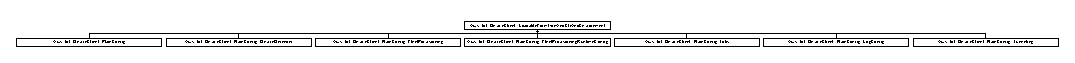
\includegraphics[height=0.403023cm]{class_aws_1_1_iot_1_1_device_client_1_1_loadable_from_json_and_cli_and_environment}
\end{center}
\end{figure}
\subsection*{Public Member Functions}
\begin{DoxyCompactItemize}
\item 
\mbox{\Hypertarget{class_aws_1_1_iot_1_1_device_client_1_1_loadable_from_json_and_cli_and_environment_adaa0942506f6322df4b46bb7cf79cdcf}\label{class_aws_1_1_iot_1_1_device_client_1_1_loadable_from_json_and_cli_and_environment_adaa0942506f6322df4b46bb7cf79cdcf}} 
virtual bool {\bfseries Load\+From\+Json} (const Crt\+::\+Json\+View \&json)=0
\item 
\mbox{\Hypertarget{class_aws_1_1_iot_1_1_device_client_1_1_loadable_from_json_and_cli_and_environment_abbf0e30b0d353c5a89c021ee3e89d8d2}\label{class_aws_1_1_iot_1_1_device_client_1_1_loadable_from_json_and_cli_and_environment_abbf0e30b0d353c5a89c021ee3e89d8d2}} 
virtual bool {\bfseries Load\+From\+Cli\+Args} (const Cli\+Args \&cli\+Args)=0
\item 
\mbox{\Hypertarget{class_aws_1_1_iot_1_1_device_client_1_1_loadable_from_json_and_cli_and_environment_ab5ea0846ea91b7ceb472a48c7f4b49ad}\label{class_aws_1_1_iot_1_1_device_client_1_1_loadable_from_json_and_cli_and_environment_ab5ea0846ea91b7ceb472a48c7f4b49ad}} 
virtual bool {\bfseries Load\+From\+Environment} ()=0
\item 
\mbox{\Hypertarget{class_aws_1_1_iot_1_1_device_client_1_1_loadable_from_json_and_cli_and_environment_a260957ac4b9f9ec3be06876b6a75f129}\label{class_aws_1_1_iot_1_1_device_client_1_1_loadable_from_json_and_cli_and_environment_a260957ac4b9f9ec3be06876b6a75f129}} 
virtual bool {\bfseries Validate} () const =0
\end{DoxyCompactItemize}


The documentation for this class was generated from the following file\+:\begin{DoxyCompactItemize}
\item 
/home/\+A\+N\+T.\+A\+M\+A\+Z\+O\+N.\+C\+O\+M/lwwilkov/\+Workspace/aws-\/iot-\/device-\/client/source/config/Config.\+h\end{DoxyCompactItemize}

\hypertarget{struct_aws_1_1_iot_1_1_device_client_1_1_plain_config_1_1_log_config}{}\section{Aws\+:\+:Iot\+:\+:Device\+Client\+:\+:Plain\+Config\+:\+:Log\+Config Struct Reference}
\label{struct_aws_1_1_iot_1_1_device_client_1_1_plain_config_1_1_log_config}\index{Aws\+::\+Iot\+::\+Device\+Client\+::\+Plain\+Config\+::\+Log\+Config@{Aws\+::\+Iot\+::\+Device\+Client\+::\+Plain\+Config\+::\+Log\+Config}}
Inheritance diagram for Aws\+:\+:Iot\+:\+:Device\+Client\+:\+:Plain\+Config\+:\+:Log\+Config\+:\begin{figure}[H]
\begin{center}
\leavevmode
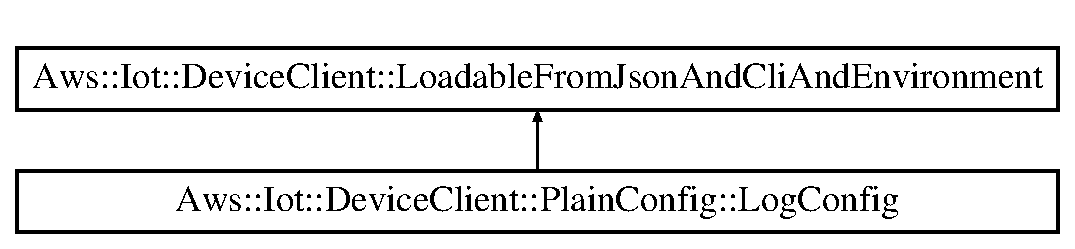
\includegraphics[height=2.000000cm]{struct_aws_1_1_iot_1_1_device_client_1_1_plain_config_1_1_log_config}
\end{center}
\end{figure}
\subsection*{Public Member Functions}
\begin{DoxyCompactItemize}
\item 
\mbox{\Hypertarget{struct_aws_1_1_iot_1_1_device_client_1_1_plain_config_1_1_log_config_ae76718f6339d1de9afe44dfcd6d19ff6}\label{struct_aws_1_1_iot_1_1_device_client_1_1_plain_config_1_1_log_config_ae76718f6339d1de9afe44dfcd6d19ff6}} 
bool {\bfseries Load\+From\+Json} (const Crt\+::\+Json\+View \&json) override
\item 
\mbox{\Hypertarget{struct_aws_1_1_iot_1_1_device_client_1_1_plain_config_1_1_log_config_a685b769bc9a58a8c0be0f02f90665e2e}\label{struct_aws_1_1_iot_1_1_device_client_1_1_plain_config_1_1_log_config_a685b769bc9a58a8c0be0f02f90665e2e}} 
bool {\bfseries Load\+From\+Cli\+Args} (const Cli\+Args \&cli\+Args) override
\item 
\mbox{\Hypertarget{struct_aws_1_1_iot_1_1_device_client_1_1_plain_config_1_1_log_config_a9918cd66a6d2366af86aa2a2f013a439}\label{struct_aws_1_1_iot_1_1_device_client_1_1_plain_config_1_1_log_config_a9918cd66a6d2366af86aa2a2f013a439}} 
bool {\bfseries Load\+From\+Environment} () override
\item 
\mbox{\Hypertarget{struct_aws_1_1_iot_1_1_device_client_1_1_plain_config_1_1_log_config_a1f63d80d33fd430212aff3564c60cd4f}\label{struct_aws_1_1_iot_1_1_device_client_1_1_plain_config_1_1_log_config_a1f63d80d33fd430212aff3564c60cd4f}} 
bool {\bfseries Validate} () const override
\item 
\mbox{\Hypertarget{struct_aws_1_1_iot_1_1_device_client_1_1_plain_config_1_1_log_config_aa4a4cd2a51c05c0ddebb7b8c73bd7ac3}\label{struct_aws_1_1_iot_1_1_device_client_1_1_plain_config_1_1_log_config_aa4a4cd2a51c05c0ddebb7b8c73bd7ac3}} 
int {\bfseries Parse\+Log\+Level} (std\+::string value)
\item 
\mbox{\Hypertarget{struct_aws_1_1_iot_1_1_device_client_1_1_plain_config_1_1_log_config_a08f9ef8c34c6d7a2b3d035cc8ab53e90}\label{struct_aws_1_1_iot_1_1_device_client_1_1_plain_config_1_1_log_config_a08f9ef8c34c6d7a2b3d035cc8ab53e90}} 
std\+::string {\bfseries Parse\+Log\+Type} (std\+::string value)
\end{DoxyCompactItemize}
\subsection*{Public Attributes}
\begin{DoxyCompactItemize}
\item 
\mbox{\Hypertarget{struct_aws_1_1_iot_1_1_device_client_1_1_plain_config_1_1_log_config_a0f7f802c9ae17476b862dca64f47ca7f}\label{struct_aws_1_1_iot_1_1_device_client_1_1_plain_config_1_1_log_config_a0f7f802c9ae17476b862dca64f47ca7f}} 
int {\bfseries log\+Level} \{3\}
\item 
\mbox{\Hypertarget{struct_aws_1_1_iot_1_1_device_client_1_1_plain_config_1_1_log_config_a44d68763fc7271528b1d23311e046a92}\label{struct_aws_1_1_iot_1_1_device_client_1_1_plain_config_1_1_log_config_a44d68763fc7271528b1d23311e046a92}} 
std\+::string {\bfseries type}
\item 
\mbox{\Hypertarget{struct_aws_1_1_iot_1_1_device_client_1_1_plain_config_1_1_log_config_a4c8ef3ccc3ef8ad6adf29305751a921b}\label{struct_aws_1_1_iot_1_1_device_client_1_1_plain_config_1_1_log_config_a4c8ef3ccc3ef8ad6adf29305751a921b}} 
std\+::string {\bfseries file}
\end{DoxyCompactItemize}
\subsection*{Static Public Attributes}
\begin{DoxyCompactItemize}
\item 
\mbox{\Hypertarget{struct_aws_1_1_iot_1_1_device_client_1_1_plain_config_1_1_log_config_a5542234e678e868c4125ad205926a4f7}\label{struct_aws_1_1_iot_1_1_device_client_1_1_plain_config_1_1_log_config_a5542234e678e868c4125ad205926a4f7}} 
static constexpr char {\bfseries L\+O\+G\+\_\+\+T\+Y\+P\+E\+\_\+\+F\+I\+LE} \mbox{[}$\,$\mbox{]} = \char`\"{}file\char`\"{}
\item 
\mbox{\Hypertarget{struct_aws_1_1_iot_1_1_device_client_1_1_plain_config_1_1_log_config_a6da5b0c5098e396d2f99168196b14084}\label{struct_aws_1_1_iot_1_1_device_client_1_1_plain_config_1_1_log_config_a6da5b0c5098e396d2f99168196b14084}} 
static constexpr char {\bfseries L\+O\+G\+\_\+\+T\+Y\+P\+E\+\_\+\+S\+T\+D\+O\+UT} \mbox{[}$\,$\mbox{]} = \char`\"{}stdout\char`\"{}
\item 
\mbox{\Hypertarget{struct_aws_1_1_iot_1_1_device_client_1_1_plain_config_1_1_log_config_ad690ba98c24c6a0f72b3afd0eb8201b3}\label{struct_aws_1_1_iot_1_1_device_client_1_1_plain_config_1_1_log_config_ad690ba98c24c6a0f72b3afd0eb8201b3}} 
static constexpr char {\bfseries C\+L\+I\+\_\+\+L\+O\+G\+\_\+\+L\+E\+V\+EL} \mbox{[}$\,$\mbox{]} = \char`\"{}-\/-\/log-\/level\char`\"{}
\item 
\mbox{\Hypertarget{struct_aws_1_1_iot_1_1_device_client_1_1_plain_config_1_1_log_config_a68113a412eb49cb9821fa81bc3fd1c1f}\label{struct_aws_1_1_iot_1_1_device_client_1_1_plain_config_1_1_log_config_a68113a412eb49cb9821fa81bc3fd1c1f}} 
static constexpr char {\bfseries C\+L\+I\+\_\+\+L\+O\+G\+\_\+\+T\+Y\+PE} \mbox{[}$\,$\mbox{]} = \char`\"{}-\/-\/log-\/type\char`\"{}
\item 
\mbox{\Hypertarget{struct_aws_1_1_iot_1_1_device_client_1_1_plain_config_1_1_log_config_a2b40b5839d3ff036eec1588b33600389}\label{struct_aws_1_1_iot_1_1_device_client_1_1_plain_config_1_1_log_config_a2b40b5839d3ff036eec1588b33600389}} 
static constexpr char {\bfseries C\+L\+I\+\_\+\+L\+O\+G\+\_\+\+F\+I\+LE} \mbox{[}$\,$\mbox{]} = \char`\"{}-\/-\/log-\/file\char`\"{}
\item 
\mbox{\Hypertarget{struct_aws_1_1_iot_1_1_device_client_1_1_plain_config_1_1_log_config_a161f4ed4d521bad2e0bae1ec0c7a59a0}\label{struct_aws_1_1_iot_1_1_device_client_1_1_plain_config_1_1_log_config_a161f4ed4d521bad2e0bae1ec0c7a59a0}} 
static constexpr char {\bfseries J\+S\+O\+N\+\_\+\+K\+E\+Y\+\_\+\+L\+O\+G\+\_\+\+L\+E\+V\+EL} \mbox{[}$\,$\mbox{]} = \char`\"{}level\char`\"{}
\item 
\mbox{\Hypertarget{struct_aws_1_1_iot_1_1_device_client_1_1_plain_config_1_1_log_config_a79a5c1c62a2f129fcfe1be00f71fba7d}\label{struct_aws_1_1_iot_1_1_device_client_1_1_plain_config_1_1_log_config_a79a5c1c62a2f129fcfe1be00f71fba7d}} 
static constexpr char {\bfseries J\+S\+O\+N\+\_\+\+K\+E\+Y\+\_\+\+L\+O\+G\+\_\+\+T\+Y\+PE} \mbox{[}$\,$\mbox{]} = \char`\"{}type\char`\"{}
\item 
\mbox{\Hypertarget{struct_aws_1_1_iot_1_1_device_client_1_1_plain_config_1_1_log_config_ab6a4e5f12c8858fa2c39941edabb7fc6}\label{struct_aws_1_1_iot_1_1_device_client_1_1_plain_config_1_1_log_config_ab6a4e5f12c8858fa2c39941edabb7fc6}} 
static constexpr char {\bfseries J\+S\+O\+N\+\_\+\+K\+E\+Y\+\_\+\+L\+O\+G\+\_\+\+F\+I\+LE} \mbox{[}$\,$\mbox{]} = \char`\"{}file\char`\"{}
\end{DoxyCompactItemize}


The documentation for this struct was generated from the following files\+:\begin{DoxyCompactItemize}
\item 
/home/\+A\+N\+T.\+A\+M\+A\+Z\+O\+N.\+C\+O\+M/lwwilkov/\+Workspace/aws-\/iot-\/device-\/client/source/config/Config.\+h\item 
/home/\+A\+N\+T.\+A\+M\+A\+Z\+O\+N.\+C\+O\+M/lwwilkov/\+Workspace/aws-\/iot-\/device-\/client/source/config/Config.\+cpp\end{DoxyCompactItemize}

\hypertarget{class_aws_1_1_iot_1_1_device_client_1_1_logging_1_1_logger}{}\section{Aws\+:\+:Iot\+:\+:Device\+Client\+:\+:Logging\+:\+:Logger Class Reference}
\label{class_aws_1_1_iot_1_1_device_client_1_1_logging_1_1_logger}\index{Aws\+::\+Iot\+::\+Device\+Client\+::\+Logging\+::\+Logger@{Aws\+::\+Iot\+::\+Device\+Client\+::\+Logging\+::\+Logger}}


Interface representing essential methods that must provided by any underlying Log generating implementation.  




{\ttfamily \#include $<$Logger.\+h$>$}

Inheritance diagram for Aws\+:\+:Iot\+:\+:Device\+Client\+:\+:Logging\+:\+:Logger\+:\begin{figure}[H]
\begin{center}
\leavevmode
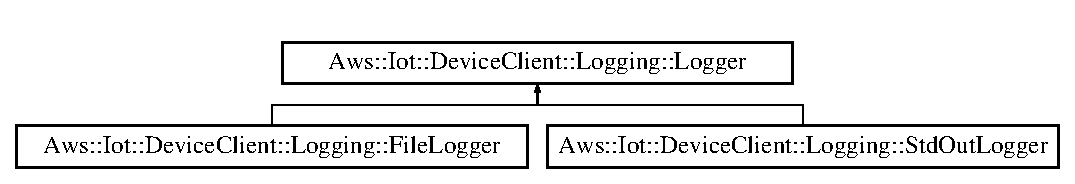
\includegraphics[height=2.000000cm]{class_aws_1_1_iot_1_1_device_client_1_1_logging_1_1_logger}
\end{center}
\end{figure}
\subsection*{Public Member Functions}
\begin{DoxyCompactItemize}
\item 
virtual void \hyperlink{class_aws_1_1_iot_1_1_device_client_1_1_logging_1_1_logger_aee99f5d53316cb0dba7f517475f01443}{vlog} (Log\+Level level, const char $\ast$tag, std\+::chrono\+::time\+\_\+point$<$ std\+::chrono\+::system\+\_\+clock $>$ t, const char $\ast$message, va\+\_\+list args)
\begin{DoxyCompactList}\small\item\em Formats the provided log message against variadic arguments and then passes the message to the underlying logger implementation for processing. \end{DoxyCompactList}\item 
void \hyperlink{class_aws_1_1_iot_1_1_device_client_1_1_logging_1_1_logger_a2100929095644e9f5de260aca46f6142}{error} (const char $\ast$tag, std\+::chrono\+::time\+\_\+point$<$ std\+::chrono\+::system\+\_\+clock $>$ t, const char $\ast$message,...)
\begin{DoxyCompactList}\small\item\em Log the message at the E\+R\+R\+OR level. If the current logging level is less than E\+R\+R\+OR, then this is a N\+O\+OP. \end{DoxyCompactList}\item 
void \hyperlink{class_aws_1_1_iot_1_1_device_client_1_1_logging_1_1_logger_af7bb64146051fcd5b801ee2ed4e619d8}{warn} (const char $\ast$tag, std\+::chrono\+::time\+\_\+point$<$ std\+::chrono\+::system\+\_\+clock $>$ t, const char $\ast$message,...)
\begin{DoxyCompactList}\small\item\em Log the message at the W\+A\+RN level. If the current logging level is less than W\+A\+RN, then this is a N\+O\+OP. \end{DoxyCompactList}\item 
void \hyperlink{class_aws_1_1_iot_1_1_device_client_1_1_logging_1_1_logger_a9ac04311763fcffa096eb062ba479897}{info} (const char $\ast$tag, std\+::chrono\+::time\+\_\+point$<$ std\+::chrono\+::system\+\_\+clock $>$ t, const char $\ast$message,...)
\begin{DoxyCompactList}\small\item\em Log the message at the I\+N\+FO level. If the current logging level is less than I\+N\+FO, then this is a N\+O\+OP. \end{DoxyCompactList}\item 
void \hyperlink{class_aws_1_1_iot_1_1_device_client_1_1_logging_1_1_logger_ad64e2decc9c73a45717f1d87bb3d404a}{debug} (const char $\ast$tag, std\+::chrono\+::time\+\_\+point$<$ std\+::chrono\+::system\+\_\+clock $>$ t, const char $\ast$message,...)
\begin{DoxyCompactList}\small\item\em Log the message at the D\+E\+B\+UG level. If the current logging level is less than D\+E\+B\+UG, then this is a N\+O\+OP. \end{DoxyCompactList}\item 
virtual bool \hyperlink{class_aws_1_1_iot_1_1_device_client_1_1_logging_1_1_logger_ad42e38afcd7402f5dc1213b2f0b96961}{start} (const \hyperlink{struct_aws_1_1_iot_1_1_device_client_1_1_plain_config}{Plain\+Config} \&config)=0
\begin{DoxyCompactList}\small\item\em Starts the underlying logger implementation\textquotesingle{}s logging behavior. \end{DoxyCompactList}\item 
\mbox{\Hypertarget{class_aws_1_1_iot_1_1_device_client_1_1_logging_1_1_logger_a1bfa1932649b6189dc685a9ba943fef8}\label{class_aws_1_1_iot_1_1_device_client_1_1_logging_1_1_logger_a1bfa1932649b6189dc685a9ba943fef8}} 
virtual void \hyperlink{class_aws_1_1_iot_1_1_device_client_1_1_logging_1_1_logger_a1bfa1932649b6189dc685a9ba943fef8}{stop} ()=0
\begin{DoxyCompactList}\small\item\em Attempts to stop the \hyperlink{class_aws_1_1_iot_1_1_device_client_1_1_logging_1_1_logger}{Logger} implementation from writing any additional log messages, likely to switch to a different logger implementation. \end{DoxyCompactList}\item 
\mbox{\Hypertarget{class_aws_1_1_iot_1_1_device_client_1_1_logging_1_1_logger_a0531d2c3daf665bb5751f2f219d3ca6e}\label{class_aws_1_1_iot_1_1_device_client_1_1_logging_1_1_logger_a0531d2c3daf665bb5751f2f219d3ca6e}} 
virtual void \hyperlink{class_aws_1_1_iot_1_1_device_client_1_1_logging_1_1_logger_a0531d2c3daf665bb5751f2f219d3ca6e}{shutdown} ()=0
\begin{DoxyCompactList}\small\item\em Notifies the \hyperlink{class_aws_1_1_iot_1_1_device_client_1_1_logging_1_1_logger}{Logger} implementation that any queued logs should be dumped to output and the logger should shut itself down. \end{DoxyCompactList}\item 
virtual std\+::unique\+\_\+ptr$<$ \hyperlink{class_aws_1_1_iot_1_1_device_client_1_1_logging_1_1_log_queue}{Log\+Queue} $>$ \hyperlink{class_aws_1_1_iot_1_1_device_client_1_1_logging_1_1_logger_a39f3326be17f9ed4b1385f057134774d}{take\+Log\+Queue} ()=0
\begin{DoxyCompactList}\small\item\em Removes the \hyperlink{class_aws_1_1_iot_1_1_device_client_1_1_logging_1_1_log_queue}{Log\+Queue} from the logger implementation so it can be passed to another logger implementation for processing. \end{DoxyCompactList}\item 
virtual void \hyperlink{class_aws_1_1_iot_1_1_device_client_1_1_logging_1_1_logger_a6b80ca4200fbc58bb2994ef4319ea822}{set\+Log\+Queue} (std\+::unique\+\_\+ptr$<$ \hyperlink{class_aws_1_1_iot_1_1_device_client_1_1_logging_1_1_log_queue}{Log\+Queue} $>$ log\+Queue)=0
\begin{DoxyCompactList}\small\item\em Passes a \hyperlink{class_aws_1_1_iot_1_1_device_client_1_1_logging_1_1_log_queue}{Log\+Queue} to the logger implementation. Typically used if the logger implementation is being changed. \end{DoxyCompactList}\item 
virtual void \hyperlink{class_aws_1_1_iot_1_1_device_client_1_1_logging_1_1_logger_a4743383e9c69bec10ba970dc4394781e}{flush} ()=0
\begin{DoxyCompactList}\small\item\em Flush the log output from the queue synchronously. \end{DoxyCompactList}\end{DoxyCompactItemize}
\subsection*{Protected Member Functions}
\begin{DoxyCompactItemize}
\item 
virtual void \hyperlink{class_aws_1_1_iot_1_1_device_client_1_1_logging_1_1_logger_a75acdae576e13ddd84bccb70d8fb1fef}{queue\+Log} (Log\+Level level, const char $\ast$tag, std\+::chrono\+::time\+\_\+point$<$ std\+::chrono\+::system\+\_\+clock $>$ t, std\+::string message)=0
\begin{DoxyCompactList}\small\item\em Implemented by the underlying logger implementation to pass responsibility for managing the log message from the \hyperlink{class_aws_1_1_iot_1_1_device_client_1_1_logging_1_1_logger}{Logger} interface to the logger implementation. \end{DoxyCompactList}\item 
void \hyperlink{class_aws_1_1_iot_1_1_device_client_1_1_logging_1_1_logger_a01b35eb1221e3bdcf744da4954f11cb2}{set\+Log\+Level} (int level)
\begin{DoxyCompactList}\small\item\em Sets the level of the \hyperlink{class_aws_1_1_iot_1_1_device_client_1_1_logging_1_1_logger}{Logger} implementation (D\+E\+B\+UG, I\+N\+FO, W\+A\+RN, E\+R\+R\+OR) \end{DoxyCompactList}\end{DoxyCompactItemize}
\subsection*{Protected Attributes}
\begin{DoxyCompactItemize}
\item 
\mbox{\Hypertarget{class_aws_1_1_iot_1_1_device_client_1_1_logging_1_1_logger_a742d59a36a966d1c593f5091e4ab6ed7}\label{class_aws_1_1_iot_1_1_device_client_1_1_logging_1_1_logger_a742d59a36a966d1c593f5091e4ab6ed7}} 
const char $\ast$ {\bfseries L\+O\+G\+G\+E\+R\+\_\+\+T\+AG} = \char`\"{}A\+WS IoT Device Client \hyperlink{class_aws_1_1_iot_1_1_device_client_1_1_logging_1_1_logger}{Logger}\char`\"{}
\item 
\mbox{\Hypertarget{class_aws_1_1_iot_1_1_device_client_1_1_logging_1_1_logger_ada1785780bfd79d789b9edaa798cf4b5}\label{class_aws_1_1_iot_1_1_device_client_1_1_logging_1_1_logger_ada1785780bfd79d789b9edaa798cf4b5}} 
int \hyperlink{class_aws_1_1_iot_1_1_device_client_1_1_logging_1_1_logger_ada1785780bfd79d789b9edaa798cf4b5}{log\+Level} = (int)Log\+Level\+::\+D\+E\+B\+UG
\begin{DoxyCompactList}\small\item\em The runtime log level for the IoT Device Client. \end{DoxyCompactList}\end{DoxyCompactItemize}


\subsection{Detailed Description}
Interface representing essential methods that must provided by any underlying Log generating implementation. 

The \hyperlink{class_aws_1_1_iot_1_1_device_client_1_1_logging_1_1_logger}{Logger} class represents an interface by which the Device Client may generate logs and write them to some desired output. The class itself provides some top level methods that handle logging levels and formatting log messages with variadic arguments. The underlying logger implementation handles actual log output generating through use of the queue\+Log method, which assumes the implementation will swiftly queue the log message and then handle output accordingly. 

\subsection{Member Function Documentation}
\mbox{\Hypertarget{class_aws_1_1_iot_1_1_device_client_1_1_logging_1_1_logger_ad64e2decc9c73a45717f1d87bb3d404a}\label{class_aws_1_1_iot_1_1_device_client_1_1_logging_1_1_logger_ad64e2decc9c73a45717f1d87bb3d404a}} 
\index{Aws\+::\+Iot\+::\+Device\+Client\+::\+Logging\+::\+Logger@{Aws\+::\+Iot\+::\+Device\+Client\+::\+Logging\+::\+Logger}!debug@{debug}}
\index{debug@{debug}!Aws\+::\+Iot\+::\+Device\+Client\+::\+Logging\+::\+Logger@{Aws\+::\+Iot\+::\+Device\+Client\+::\+Logging\+::\+Logger}}
\subsubsection{\texorpdfstring{debug()}{debug()}}
{\footnotesize\ttfamily void Aws\+::\+Iot\+::\+Device\+Client\+::\+Logging\+::\+Logger\+::debug (\begin{DoxyParamCaption}\item[{const char $\ast$}]{tag,  }\item[{std\+::chrono\+::time\+\_\+point$<$ std\+::chrono\+::system\+\_\+clock $>$}]{t,  }\item[{const char $\ast$}]{message,  }\item[{}]{... }\end{DoxyParamCaption})\hspace{0.3cm}{\ttfamily [inline]}}



Log the message at the D\+E\+B\+UG level. If the current logging level is less than D\+E\+B\+UG, then this is a N\+O\+OP. 


\begin{DoxyTemplParams}{Template Parameters}
{\em Args} & variadic number of arguments that may be passed in for formatting against the log message \\
\hline
\end{DoxyTemplParams}

\begin{DoxyParams}{Parameters}
{\em tag} & a tag indicating where in the source code the log message is coming from \\
\hline
{\em t} & a timestamp representing the time this message was created \\
\hline
{\em message} & the log message \\
\hline
{\em args} & variadic number of arguments that may be passed in for formatting against the log message \\
\hline
\end{DoxyParams}
\mbox{\Hypertarget{class_aws_1_1_iot_1_1_device_client_1_1_logging_1_1_logger_a2100929095644e9f5de260aca46f6142}\label{class_aws_1_1_iot_1_1_device_client_1_1_logging_1_1_logger_a2100929095644e9f5de260aca46f6142}} 
\index{Aws\+::\+Iot\+::\+Device\+Client\+::\+Logging\+::\+Logger@{Aws\+::\+Iot\+::\+Device\+Client\+::\+Logging\+::\+Logger}!error@{error}}
\index{error@{error}!Aws\+::\+Iot\+::\+Device\+Client\+::\+Logging\+::\+Logger@{Aws\+::\+Iot\+::\+Device\+Client\+::\+Logging\+::\+Logger}}
\subsubsection{\texorpdfstring{error()}{error()}}
{\footnotesize\ttfamily void Aws\+::\+Iot\+::\+Device\+Client\+::\+Logging\+::\+Logger\+::error (\begin{DoxyParamCaption}\item[{const char $\ast$}]{tag,  }\item[{std\+::chrono\+::time\+\_\+point$<$ std\+::chrono\+::system\+\_\+clock $>$}]{t,  }\item[{const char $\ast$}]{message,  }\item[{}]{... }\end{DoxyParamCaption})\hspace{0.3cm}{\ttfamily [inline]}}



Log the message at the E\+R\+R\+OR level. If the current logging level is less than E\+R\+R\+OR, then this is a N\+O\+OP. 


\begin{DoxyTemplParams}{Template Parameters}
{\em Args} & variadic number of arguments that may be passed in for formatting against the log message \\
\hline
\end{DoxyTemplParams}

\begin{DoxyParams}{Parameters}
{\em tag} & a tag indicating where in the source code the log message is coming from \\
\hline
{\em t} & a timestamp representing the time this message was created \\
\hline
{\em message} & the log message \\
\hline
{\em args} & variadic number of arguments that may be passed in for formatting against the log message \\
\hline
\end{DoxyParams}
\mbox{\Hypertarget{class_aws_1_1_iot_1_1_device_client_1_1_logging_1_1_logger_a4743383e9c69bec10ba970dc4394781e}\label{class_aws_1_1_iot_1_1_device_client_1_1_logging_1_1_logger_a4743383e9c69bec10ba970dc4394781e}} 
\index{Aws\+::\+Iot\+::\+Device\+Client\+::\+Logging\+::\+Logger@{Aws\+::\+Iot\+::\+Device\+Client\+::\+Logging\+::\+Logger}!flush@{flush}}
\index{flush@{flush}!Aws\+::\+Iot\+::\+Device\+Client\+::\+Logging\+::\+Logger@{Aws\+::\+Iot\+::\+Device\+Client\+::\+Logging\+::\+Logger}}
\subsubsection{\texorpdfstring{flush()}{flush()}}
{\footnotesize\ttfamily virtual void Aws\+::\+Iot\+::\+Device\+Client\+::\+Logging\+::\+Logger\+::flush (\begin{DoxyParamCaption}{ }\end{DoxyParamCaption})\hspace{0.3cm}{\ttfamily [pure virtual]}}



Flush the log output from the queue synchronously. 

This is helpful for scenarios where you need to ensure that the logs are written to disk before any other activity takes place. Note that this will not block other threads, only the thread that this is called from 

Implemented in \hyperlink{class_aws_1_1_iot_1_1_device_client_1_1_logging_1_1_file_logger_a507513cb4aca226a5ed6da292bfd915a}{Aws\+::\+Iot\+::\+Device\+Client\+::\+Logging\+::\+File\+Logger}, and \hyperlink{class_aws_1_1_iot_1_1_device_client_1_1_logging_1_1_std_out_logger_a27610c8adc232399266ef8c8f09eb46b}{Aws\+::\+Iot\+::\+Device\+Client\+::\+Logging\+::\+Std\+Out\+Logger}.

\mbox{\Hypertarget{class_aws_1_1_iot_1_1_device_client_1_1_logging_1_1_logger_a9ac04311763fcffa096eb062ba479897}\label{class_aws_1_1_iot_1_1_device_client_1_1_logging_1_1_logger_a9ac04311763fcffa096eb062ba479897}} 
\index{Aws\+::\+Iot\+::\+Device\+Client\+::\+Logging\+::\+Logger@{Aws\+::\+Iot\+::\+Device\+Client\+::\+Logging\+::\+Logger}!info@{info}}
\index{info@{info}!Aws\+::\+Iot\+::\+Device\+Client\+::\+Logging\+::\+Logger@{Aws\+::\+Iot\+::\+Device\+Client\+::\+Logging\+::\+Logger}}
\subsubsection{\texorpdfstring{info()}{info()}}
{\footnotesize\ttfamily void Aws\+::\+Iot\+::\+Device\+Client\+::\+Logging\+::\+Logger\+::info (\begin{DoxyParamCaption}\item[{const char $\ast$}]{tag,  }\item[{std\+::chrono\+::time\+\_\+point$<$ std\+::chrono\+::system\+\_\+clock $>$}]{t,  }\item[{const char $\ast$}]{message,  }\item[{}]{... }\end{DoxyParamCaption})\hspace{0.3cm}{\ttfamily [inline]}}



Log the message at the I\+N\+FO level. If the current logging level is less than I\+N\+FO, then this is a N\+O\+OP. 


\begin{DoxyTemplParams}{Template Parameters}
{\em Args} & variadic number of arguments that may be passed in for formatting against the log message \\
\hline
\end{DoxyTemplParams}

\begin{DoxyParams}{Parameters}
{\em tag} & a tag indicating where in the source code the log message is coming from \\
\hline
{\em t} & a timestamp representing the time this message was created \\
\hline
{\em message} & the log message \\
\hline
{\em args} & variadic number of arguments that may be passed in for formatting against the log message \\
\hline
\end{DoxyParams}
\mbox{\Hypertarget{class_aws_1_1_iot_1_1_device_client_1_1_logging_1_1_logger_a75acdae576e13ddd84bccb70d8fb1fef}\label{class_aws_1_1_iot_1_1_device_client_1_1_logging_1_1_logger_a75acdae576e13ddd84bccb70d8fb1fef}} 
\index{Aws\+::\+Iot\+::\+Device\+Client\+::\+Logging\+::\+Logger@{Aws\+::\+Iot\+::\+Device\+Client\+::\+Logging\+::\+Logger}!queue\+Log@{queue\+Log}}
\index{queue\+Log@{queue\+Log}!Aws\+::\+Iot\+::\+Device\+Client\+::\+Logging\+::\+Logger@{Aws\+::\+Iot\+::\+Device\+Client\+::\+Logging\+::\+Logger}}
\subsubsection{\texorpdfstring{queue\+Log()}{queueLog()}}
{\footnotesize\ttfamily virtual void Aws\+::\+Iot\+::\+Device\+Client\+::\+Logging\+::\+Logger\+::queue\+Log (\begin{DoxyParamCaption}\item[{Log\+Level}]{level,  }\item[{const char $\ast$}]{tag,  }\item[{std\+::chrono\+::time\+\_\+point$<$ std\+::chrono\+::system\+\_\+clock $>$}]{t,  }\item[{std\+::string}]{message }\end{DoxyParamCaption})\hspace{0.3cm}{\ttfamily [protected]}, {\ttfamily [pure virtual]}}



Implemented by the underlying logger implementation to pass responsibility for managing the log message from the \hyperlink{class_aws_1_1_iot_1_1_device_client_1_1_logging_1_1_logger}{Logger} interface to the logger implementation. 

This virtual method should be implemented by the underlying logger implementation to actually accept and eventually process the incoming log message. To reduce complications induced by multithreading, the underlying logger implementation should queue the message for processing by another thread if possible. 
\begin{DoxyParams}{Parameters}
{\em level} & the log level \\
\hline
{\em tag} & a tag that indicates where the log message is coming from \\
\hline
{\em t} & a timestamp representing the time the message was created \\
\hline
{\em message} & the message to log \\
\hline
\end{DoxyParams}


Implemented in \hyperlink{class_aws_1_1_iot_1_1_device_client_1_1_logging_1_1_file_logger_a549cf9783ce070e514c0f68340ae5d1c}{Aws\+::\+Iot\+::\+Device\+Client\+::\+Logging\+::\+File\+Logger}, and \hyperlink{class_aws_1_1_iot_1_1_device_client_1_1_logging_1_1_std_out_logger_a829dd9d573157d3cbc6865b38572dd85}{Aws\+::\+Iot\+::\+Device\+Client\+::\+Logging\+::\+Std\+Out\+Logger}.

\mbox{\Hypertarget{class_aws_1_1_iot_1_1_device_client_1_1_logging_1_1_logger_a01b35eb1221e3bdcf744da4954f11cb2}\label{class_aws_1_1_iot_1_1_device_client_1_1_logging_1_1_logger_a01b35eb1221e3bdcf744da4954f11cb2}} 
\index{Aws\+::\+Iot\+::\+Device\+Client\+::\+Logging\+::\+Logger@{Aws\+::\+Iot\+::\+Device\+Client\+::\+Logging\+::\+Logger}!set\+Log\+Level@{set\+Log\+Level}}
\index{set\+Log\+Level@{set\+Log\+Level}!Aws\+::\+Iot\+::\+Device\+Client\+::\+Logging\+::\+Logger@{Aws\+::\+Iot\+::\+Device\+Client\+::\+Logging\+::\+Logger}}
\subsubsection{\texorpdfstring{set\+Log\+Level()}{setLogLevel()}}
{\footnotesize\ttfamily void Aws\+::\+Iot\+::\+Device\+Client\+::\+Logging\+::\+Logger\+::set\+Log\+Level (\begin{DoxyParamCaption}\item[{int}]{level }\end{DoxyParamCaption})\hspace{0.3cm}{\ttfamily [inline]}, {\ttfamily [protected]}}



Sets the level of the \hyperlink{class_aws_1_1_iot_1_1_device_client_1_1_logging_1_1_logger}{Logger} implementation (D\+E\+B\+UG, I\+N\+FO, W\+A\+RN, E\+R\+R\+OR) 


\begin{DoxyParams}{Parameters}
{\em level} & the level to set the logger to \\
\hline
\end{DoxyParams}
\mbox{\Hypertarget{class_aws_1_1_iot_1_1_device_client_1_1_logging_1_1_logger_a6b80ca4200fbc58bb2994ef4319ea822}\label{class_aws_1_1_iot_1_1_device_client_1_1_logging_1_1_logger_a6b80ca4200fbc58bb2994ef4319ea822}} 
\index{Aws\+::\+Iot\+::\+Device\+Client\+::\+Logging\+::\+Logger@{Aws\+::\+Iot\+::\+Device\+Client\+::\+Logging\+::\+Logger}!set\+Log\+Queue@{set\+Log\+Queue}}
\index{set\+Log\+Queue@{set\+Log\+Queue}!Aws\+::\+Iot\+::\+Device\+Client\+::\+Logging\+::\+Logger@{Aws\+::\+Iot\+::\+Device\+Client\+::\+Logging\+::\+Logger}}
\subsubsection{\texorpdfstring{set\+Log\+Queue()}{setLogQueue()}}
{\footnotesize\ttfamily virtual void Aws\+::\+Iot\+::\+Device\+Client\+::\+Logging\+::\+Logger\+::set\+Log\+Queue (\begin{DoxyParamCaption}\item[{std\+::unique\+\_\+ptr$<$ \hyperlink{class_aws_1_1_iot_1_1_device_client_1_1_logging_1_1_log_queue}{Log\+Queue} $>$}]{log\+Queue }\end{DoxyParamCaption})\hspace{0.3cm}{\ttfamily [pure virtual]}}



Passes a \hyperlink{class_aws_1_1_iot_1_1_device_client_1_1_logging_1_1_log_queue}{Log\+Queue} to the logger implementation. Typically used if the logger implementation is being changed. 


\begin{DoxyParams}{Parameters}
{\em log\+Queue} & \\
\hline
\end{DoxyParams}


Implemented in \hyperlink{class_aws_1_1_iot_1_1_device_client_1_1_logging_1_1_file_logger_a42b047d2f2379638add126414690d65d}{Aws\+::\+Iot\+::\+Device\+Client\+::\+Logging\+::\+File\+Logger}, and \hyperlink{class_aws_1_1_iot_1_1_device_client_1_1_logging_1_1_std_out_logger_aa35c525dc9aa3fef0f1f244781d304ea}{Aws\+::\+Iot\+::\+Device\+Client\+::\+Logging\+::\+Std\+Out\+Logger}.

\mbox{\Hypertarget{class_aws_1_1_iot_1_1_device_client_1_1_logging_1_1_logger_ad42e38afcd7402f5dc1213b2f0b96961}\label{class_aws_1_1_iot_1_1_device_client_1_1_logging_1_1_logger_ad42e38afcd7402f5dc1213b2f0b96961}} 
\index{Aws\+::\+Iot\+::\+Device\+Client\+::\+Logging\+::\+Logger@{Aws\+::\+Iot\+::\+Device\+Client\+::\+Logging\+::\+Logger}!start@{start}}
\index{start@{start}!Aws\+::\+Iot\+::\+Device\+Client\+::\+Logging\+::\+Logger@{Aws\+::\+Iot\+::\+Device\+Client\+::\+Logging\+::\+Logger}}
\subsubsection{\texorpdfstring{start()}{start()}}
{\footnotesize\ttfamily virtual bool Aws\+::\+Iot\+::\+Device\+Client\+::\+Logging\+::\+Logger\+::start (\begin{DoxyParamCaption}\item[{const \hyperlink{struct_aws_1_1_iot_1_1_device_client_1_1_plain_config}{Plain\+Config} \&}]{config }\end{DoxyParamCaption})\hspace{0.3cm}{\ttfamily [pure virtual]}}



Starts the underlying logger implementation\textquotesingle{}s logging behavior. 


\begin{DoxyParams}{Parameters}
{\em config} & the config data passed in from the C\+LI and J\+S\+ON \\
\hline
\end{DoxyParams}
\begin{DoxyReturn}{Returns}
true if it is able to start successfully, false otherwise 
\end{DoxyReturn}


Implemented in \hyperlink{class_aws_1_1_iot_1_1_device_client_1_1_logging_1_1_file_logger_ac9373269d6d5c7a5ee1ba896182c97ff}{Aws\+::\+Iot\+::\+Device\+Client\+::\+Logging\+::\+File\+Logger}, and \hyperlink{class_aws_1_1_iot_1_1_device_client_1_1_logging_1_1_std_out_logger_aa27086cd009717d85b957ef1740b14e9}{Aws\+::\+Iot\+::\+Device\+Client\+::\+Logging\+::\+Std\+Out\+Logger}.

\mbox{\Hypertarget{class_aws_1_1_iot_1_1_device_client_1_1_logging_1_1_logger_a39f3326be17f9ed4b1385f057134774d}\label{class_aws_1_1_iot_1_1_device_client_1_1_logging_1_1_logger_a39f3326be17f9ed4b1385f057134774d}} 
\index{Aws\+::\+Iot\+::\+Device\+Client\+::\+Logging\+::\+Logger@{Aws\+::\+Iot\+::\+Device\+Client\+::\+Logging\+::\+Logger}!take\+Log\+Queue@{take\+Log\+Queue}}
\index{take\+Log\+Queue@{take\+Log\+Queue}!Aws\+::\+Iot\+::\+Device\+Client\+::\+Logging\+::\+Logger@{Aws\+::\+Iot\+::\+Device\+Client\+::\+Logging\+::\+Logger}}
\subsubsection{\texorpdfstring{take\+Log\+Queue()}{takeLogQueue()}}
{\footnotesize\ttfamily virtual std\+::unique\+\_\+ptr$<$\hyperlink{class_aws_1_1_iot_1_1_device_client_1_1_logging_1_1_log_queue}{Log\+Queue}$>$ Aws\+::\+Iot\+::\+Device\+Client\+::\+Logging\+::\+Logger\+::take\+Log\+Queue (\begin{DoxyParamCaption}{ }\end{DoxyParamCaption})\hspace{0.3cm}{\ttfamily [pure virtual]}}



Removes the \hyperlink{class_aws_1_1_iot_1_1_device_client_1_1_logging_1_1_log_queue}{Log\+Queue} from the logger implementation so it can be passed to another logger implementation for processing. 

\begin{DoxyReturn}{Returns}
a unique\+\_\+ptr$<$\+Log\+Queue$>$ 
\end{DoxyReturn}


Implemented in \hyperlink{class_aws_1_1_iot_1_1_device_client_1_1_logging_1_1_file_logger_a5c55467d8f46332d6ef2acde379df2f7}{Aws\+::\+Iot\+::\+Device\+Client\+::\+Logging\+::\+File\+Logger}, and \hyperlink{class_aws_1_1_iot_1_1_device_client_1_1_logging_1_1_std_out_logger_acff57144a637686b21f27aa0da9628a2}{Aws\+::\+Iot\+::\+Device\+Client\+::\+Logging\+::\+Std\+Out\+Logger}.

\mbox{\Hypertarget{class_aws_1_1_iot_1_1_device_client_1_1_logging_1_1_logger_aee99f5d53316cb0dba7f517475f01443}\label{class_aws_1_1_iot_1_1_device_client_1_1_logging_1_1_logger_aee99f5d53316cb0dba7f517475f01443}} 
\index{Aws\+::\+Iot\+::\+Device\+Client\+::\+Logging\+::\+Logger@{Aws\+::\+Iot\+::\+Device\+Client\+::\+Logging\+::\+Logger}!vlog@{vlog}}
\index{vlog@{vlog}!Aws\+::\+Iot\+::\+Device\+Client\+::\+Logging\+::\+Logger@{Aws\+::\+Iot\+::\+Device\+Client\+::\+Logging\+::\+Logger}}
\subsubsection{\texorpdfstring{vlog()}{vlog()}}
{\footnotesize\ttfamily virtual void Aws\+::\+Iot\+::\+Device\+Client\+::\+Logging\+::\+Logger\+::vlog (\begin{DoxyParamCaption}\item[{Log\+Level}]{level,  }\item[{const char $\ast$}]{tag,  }\item[{std\+::chrono\+::time\+\_\+point$<$ std\+::chrono\+::system\+\_\+clock $>$}]{t,  }\item[{const char $\ast$}]{message,  }\item[{va\+\_\+list}]{args }\end{DoxyParamCaption})\hspace{0.3cm}{\ttfamily [inline]}, {\ttfamily [virtual]}}



Formats the provided log message against variadic arguments and then passes the message to the underlying logger implementation for processing. 


\begin{DoxyParams}{Parameters}
{\em level} & the log level \\
\hline
{\em tag} & a tag that indicates where the log message is coming from \\
\hline
{\em t} & a timestamp representing the time the message was created \\
\hline
{\em message} & the message to log \\
\hline
{\em ...} & a variadic number of arguments that will be formatted against the log message \\
\hline
\end{DoxyParams}
\mbox{\Hypertarget{class_aws_1_1_iot_1_1_device_client_1_1_logging_1_1_logger_af7bb64146051fcd5b801ee2ed4e619d8}\label{class_aws_1_1_iot_1_1_device_client_1_1_logging_1_1_logger_af7bb64146051fcd5b801ee2ed4e619d8}} 
\index{Aws\+::\+Iot\+::\+Device\+Client\+::\+Logging\+::\+Logger@{Aws\+::\+Iot\+::\+Device\+Client\+::\+Logging\+::\+Logger}!warn@{warn}}
\index{warn@{warn}!Aws\+::\+Iot\+::\+Device\+Client\+::\+Logging\+::\+Logger@{Aws\+::\+Iot\+::\+Device\+Client\+::\+Logging\+::\+Logger}}
\subsubsection{\texorpdfstring{warn()}{warn()}}
{\footnotesize\ttfamily void Aws\+::\+Iot\+::\+Device\+Client\+::\+Logging\+::\+Logger\+::warn (\begin{DoxyParamCaption}\item[{const char $\ast$}]{tag,  }\item[{std\+::chrono\+::time\+\_\+point$<$ std\+::chrono\+::system\+\_\+clock $>$}]{t,  }\item[{const char $\ast$}]{message,  }\item[{}]{... }\end{DoxyParamCaption})\hspace{0.3cm}{\ttfamily [inline]}}



Log the message at the W\+A\+RN level. If the current logging level is less than W\+A\+RN, then this is a N\+O\+OP. 


\begin{DoxyTemplParams}{Template Parameters}
{\em Args} & variadic number of arguments that may be passed in for formatting against the log message \\
\hline
\end{DoxyTemplParams}

\begin{DoxyParams}{Parameters}
{\em tag} & a tag indicating where in the source code the log message is coming from \\
\hline
{\em t} & a timestamp representing the time this message was created \\
\hline
{\em message} & the log message \\
\hline
{\em args} & variadic number of arguments that may be passed in for formatting against the log message \\
\hline
\end{DoxyParams}


The documentation for this class was generated from the following file\+:\begin{DoxyCompactItemize}
\item 
/home/\+A\+N\+T.\+A\+M\+A\+Z\+O\+N.\+C\+O\+M/lwwilkov/\+Workspace/aws-\/iot-\/device-\/client/source/logging/Logger.\+h\end{DoxyCompactItemize}

\hypertarget{class_aws_1_1_iot_1_1_device_client_1_1_logging_1_1_logger_factory}{}\doxysection{Aws\+::Iot\+::Device\+Client\+::Logging\+::Logger\+Factory Class Reference}
\label{class_aws_1_1_iot_1_1_device_client_1_1_logging_1_1_logger_factory}\index{Aws::Iot::DeviceClient::Logging::LoggerFactory@{Aws::Iot::DeviceClient::Logging::LoggerFactory}}


Factory-\/style class used for instantiation of the logger implementation and access to logging features.  




{\ttfamily \#include $<$Logger\+Factory.\+h$>$}

\doxysubsection*{Static Public Member Functions}
\begin{DoxyCompactItemize}
\item 
static std\+::shared\+\_\+ptr$<$ \mbox{\hyperlink{class_aws_1_1_iot_1_1_device_client_1_1_logging_1_1_logger}{Logger}} $>$ \mbox{\hyperlink{class_aws_1_1_iot_1_1_device_client_1_1_logging_1_1_logger_factory_aa3aeb2ab09afe3977d3a4b273a1406ae}{get\+Logger\+Instance}} ()
\begin{DoxyCompactList}\small\item\em Returns the active logger instance. \end{DoxyCompactList}\item 
static bool \mbox{\hyperlink{class_aws_1_1_iot_1_1_device_client_1_1_logging_1_1_logger_factory_aa653d2356cf9852d3dd07a3f1017393f}{reconfigure}} (const \mbox{\hyperlink{struct_aws_1_1_iot_1_1_device_client_1_1_plain_config}{Plain\+Config}} \&config)
\begin{DoxyCompactList}\small\item\em Reconfigure the logger to use a new set of settings. This may include changing the log level or switching between logger implementations. \end{DoxyCompactList}\end{DoxyCompactItemize}
\doxysubsection*{Static Private Attributes}
\begin{DoxyCompactItemize}
\item 
\mbox{\Hypertarget{class_aws_1_1_iot_1_1_device_client_1_1_logging_1_1_logger_factory_ab1a8c22c64747cdc96dd69d889557f49}\label{class_aws_1_1_iot_1_1_device_client_1_1_logging_1_1_logger_factory_ab1a8c22c64747cdc96dd69d889557f49}} 
static constexpr char {\bfseries T\+AG} \mbox{[}$\,$\mbox{]} = \char`\"{}Logger\+Factory.\+cpp\char`\"{}
\item 
\mbox{\Hypertarget{class_aws_1_1_iot_1_1_device_client_1_1_logging_1_1_logger_factory_a2e578976f1980624ab0c79c42bb3af5f}\label{class_aws_1_1_iot_1_1_device_client_1_1_logging_1_1_logger_factory_a2e578976f1980624ab0c79c42bb3af5f}} 
static std\+::shared\+\_\+ptr$<$ \mbox{\hyperlink{class_aws_1_1_iot_1_1_device_client_1_1_logging_1_1_logger}{Logger}} $>$ \mbox{\hyperlink{class_aws_1_1_iot_1_1_device_client_1_1_logging_1_1_logger_factory_a2e578976f1980624ab0c79c42bb3af5f}{logger}} = shared\+\_\+ptr$<$\mbox{\hyperlink{class_aws_1_1_iot_1_1_device_client_1_1_logging_1_1_logger}{Logger}}$>$(new \mbox{\hyperlink{class_aws_1_1_iot_1_1_device_client_1_1_logging_1_1_std_out_logger}{Std\+Out\+Logger}}())
\begin{DoxyCompactList}\small\item\em The logger implementation. \end{DoxyCompactList}\end{DoxyCompactItemize}


\doxysubsection{Detailed Description}
Factory-\/style class used for instantiation of the logger implementation and access to logging features. 

This class is intended to provide a layer of abstraction between the Device Client and the actual logger implementation. 

\doxysubsection{Member Function Documentation}
\mbox{\Hypertarget{class_aws_1_1_iot_1_1_device_client_1_1_logging_1_1_logger_factory_aa3aeb2ab09afe3977d3a4b273a1406ae}\label{class_aws_1_1_iot_1_1_device_client_1_1_logging_1_1_logger_factory_aa3aeb2ab09afe3977d3a4b273a1406ae}} 
\index{Aws::Iot::DeviceClient::Logging::LoggerFactory@{Aws::Iot::DeviceClient::Logging::LoggerFactory}!getLoggerInstance@{getLoggerInstance}}
\index{getLoggerInstance@{getLoggerInstance}!Aws::Iot::DeviceClient::Logging::LoggerFactory@{Aws::Iot::DeviceClient::Logging::LoggerFactory}}
\doxysubsubsection{\texorpdfstring{getLoggerInstance()}{getLoggerInstance()}}
{\footnotesize\ttfamily shared\+\_\+ptr$<$ \mbox{\hyperlink{class_aws_1_1_iot_1_1_device_client_1_1_logging_1_1_logger}{Logger}} $>$ Logger\+Factory\+::get\+Logger\+Instance (\begin{DoxyParamCaption}{ }\end{DoxyParamCaption})\hspace{0.3cm}{\ttfamily [static]}}



Returns the active logger instance. 

\begin{DoxyReturn}{Returns}
an instance of \mbox{\hyperlink{class_aws_1_1_iot_1_1_device_client_1_1_logging_1_1_logger}{Logger}} 
\end{DoxyReturn}
\mbox{\Hypertarget{class_aws_1_1_iot_1_1_device_client_1_1_logging_1_1_logger_factory_aa653d2356cf9852d3dd07a3f1017393f}\label{class_aws_1_1_iot_1_1_device_client_1_1_logging_1_1_logger_factory_aa653d2356cf9852d3dd07a3f1017393f}} 
\index{Aws::Iot::DeviceClient::Logging::LoggerFactory@{Aws::Iot::DeviceClient::Logging::LoggerFactory}!reconfigure@{reconfigure}}
\index{reconfigure@{reconfigure}!Aws::Iot::DeviceClient::Logging::LoggerFactory@{Aws::Iot::DeviceClient::Logging::LoggerFactory}}
\doxysubsubsection{\texorpdfstring{reconfigure()}{reconfigure()}}
{\footnotesize\ttfamily bool Logger\+Factory\+::reconfigure (\begin{DoxyParamCaption}\item[{const \mbox{\hyperlink{struct_aws_1_1_iot_1_1_device_client_1_1_plain_config}{Plain\+Config}} \&}]{config }\end{DoxyParamCaption})\hspace{0.3cm}{\ttfamily [static]}}



Reconfigure the logger to use a new set of settings. This may include changing the log level or switching between logger implementations. 


\begin{DoxyParams}{Parameters}
{\em config} & \\
\hline
\end{DoxyParams}
\begin{DoxyReturn}{Returns}

\end{DoxyReturn}


The documentation for this class was generated from the following files\+:\begin{DoxyCompactItemize}
\item 
/home/runner/work/aws-\/iot-\/device-\/client/aws-\/iot-\/device-\/client/source/logging/Logger\+Factory.\+h\item 
/home/runner/work/aws-\/iot-\/device-\/client/aws-\/iot-\/device-\/client/source/logging/Logger\+Factory.\+cpp\end{DoxyCompactItemize}

\hypertarget{class_aws_1_1_iot_1_1_device_client_1_1_logging_1_1_log_message}{}\section{Aws\+:\+:Iot\+:\+:Device\+Client\+:\+:Logging\+:\+:Log\+Message Class Reference}
\label{class_aws_1_1_iot_1_1_device_client_1_1_logging_1_1_log_message}\index{Aws\+::\+Iot\+::\+Device\+Client\+::\+Logging\+::\+Log\+Message@{Aws\+::\+Iot\+::\+Device\+Client\+::\+Logging\+::\+Log\+Message}}


Represents all data that a \hyperlink{class_aws_1_1_iot_1_1_device_client_1_1_logging_1_1_logger}{Logger} implementation requires to log data, including a Log\+Level, a tag indicating the source of the log message, a time when the message was generated, and the associated message.  




{\ttfamily \#include $<$Log\+Message.\+h$>$}

\subsection*{Public Member Functions}
\begin{DoxyCompactItemize}
\item 
\mbox{\Hypertarget{class_aws_1_1_iot_1_1_device_client_1_1_logging_1_1_log_message_abdaf457e13704aa4afa4047c5aa55865}\label{class_aws_1_1_iot_1_1_device_client_1_1_logging_1_1_log_message_abdaf457e13704aa4afa4047c5aa55865}} 
{\bfseries Log\+Message} (Log\+Level \hyperlink{class_aws_1_1_iot_1_1_device_client_1_1_logging_1_1_log_message_a088cb79700c2bdaee0f2855963dead08}{level}, std\+::string \hyperlink{class_aws_1_1_iot_1_1_device_client_1_1_logging_1_1_log_message_a751caf3538bd2d0c4c5ba8b2a160699c}{tag}, std\+::chrono\+::time\+\_\+point$<$ std\+::chrono\+::system\+\_\+clock $>$ \hyperlink{class_aws_1_1_iot_1_1_device_client_1_1_logging_1_1_log_message_ac527ebc5e1b1292741d830c1e5096cb9}{time}, std\+::string \hyperlink{class_aws_1_1_iot_1_1_device_client_1_1_logging_1_1_log_message_aef2c076d9c6cdf6890b71a63e4e02fc8}{message})
\item 
Log\+Level \hyperlink{class_aws_1_1_iot_1_1_device_client_1_1_logging_1_1_log_message_aca1e4e5b8ff937fd35745716f7d62bc8}{get\+Level} ()
\begin{DoxyCompactList}\small\item\em Returns the Log\+Level of the message. \end{DoxyCompactList}\item 
std\+::string \hyperlink{class_aws_1_1_iot_1_1_device_client_1_1_logging_1_1_log_message_a32d0716b00cdd136e490e09ac05787a2}{get\+Tag} ()
\begin{DoxyCompactList}\small\item\em Returns the message tag. \end{DoxyCompactList}\item 
std\+::chrono\+::time\+\_\+point$<$ std\+::chrono\+::system\+\_\+clock $>$ \hyperlink{class_aws_1_1_iot_1_1_device_client_1_1_logging_1_1_log_message_adaa5edba4e124584c6fe597ed76f90b1}{get\+Time} ()
\begin{DoxyCompactList}\small\item\em Returns the time that the message was generated. \end{DoxyCompactList}\item 
std\+::string \& \hyperlink{class_aws_1_1_iot_1_1_device_client_1_1_logging_1_1_log_message_af02a48506f5eb6e4023666d2d6f8a280}{get\+Message} ()
\begin{DoxyCompactList}\small\item\em Returns the log message. \end{DoxyCompactList}\end{DoxyCompactItemize}
\subsection*{Private Attributes}
\begin{DoxyCompactItemize}
\item 
\mbox{\Hypertarget{class_aws_1_1_iot_1_1_device_client_1_1_logging_1_1_log_message_a088cb79700c2bdaee0f2855963dead08}\label{class_aws_1_1_iot_1_1_device_client_1_1_logging_1_1_log_message_a088cb79700c2bdaee0f2855963dead08}} 
Log\+Level \hyperlink{class_aws_1_1_iot_1_1_device_client_1_1_logging_1_1_log_message_a088cb79700c2bdaee0f2855963dead08}{level}
\begin{DoxyCompactList}\small\item\em The Log\+Level \mbox{[}D\+E\+B\+UG, I\+N\+FO, W\+A\+RN, E\+R\+R\+OR\mbox{]}. \end{DoxyCompactList}\item 
\mbox{\Hypertarget{class_aws_1_1_iot_1_1_device_client_1_1_logging_1_1_log_message_a751caf3538bd2d0c4c5ba8b2a160699c}\label{class_aws_1_1_iot_1_1_device_client_1_1_logging_1_1_log_message_a751caf3538bd2d0c4c5ba8b2a160699c}} 
std\+::string \hyperlink{class_aws_1_1_iot_1_1_device_client_1_1_logging_1_1_log_message_a751caf3538bd2d0c4c5ba8b2a160699c}{tag}
\begin{DoxyCompactList}\small\item\em A tag used to indicate the source of the log message. \end{DoxyCompactList}\item 
\mbox{\Hypertarget{class_aws_1_1_iot_1_1_device_client_1_1_logging_1_1_log_message_ac527ebc5e1b1292741d830c1e5096cb9}\label{class_aws_1_1_iot_1_1_device_client_1_1_logging_1_1_log_message_ac527ebc5e1b1292741d830c1e5096cb9}} 
std\+::chrono\+::time\+\_\+point$<$ std\+::chrono\+::system\+\_\+clock $>$ \hyperlink{class_aws_1_1_iot_1_1_device_client_1_1_logging_1_1_log_message_ac527ebc5e1b1292741d830c1e5096cb9}{time}
\begin{DoxyCompactList}\small\item\em The time that the message was logged. \end{DoxyCompactList}\item 
\mbox{\Hypertarget{class_aws_1_1_iot_1_1_device_client_1_1_logging_1_1_log_message_aef2c076d9c6cdf6890b71a63e4e02fc8}\label{class_aws_1_1_iot_1_1_device_client_1_1_logging_1_1_log_message_aef2c076d9c6cdf6890b71a63e4e02fc8}} 
std\+::string \hyperlink{class_aws_1_1_iot_1_1_device_client_1_1_logging_1_1_log_message_aef2c076d9c6cdf6890b71a63e4e02fc8}{message}
\begin{DoxyCompactList}\small\item\em The message to be logged. \end{DoxyCompactList}\end{DoxyCompactItemize}


\subsection{Detailed Description}
Represents all data that a \hyperlink{class_aws_1_1_iot_1_1_device_client_1_1_logging_1_1_logger}{Logger} implementation requires to log data, including a Log\+Level, a tag indicating the source of the log message, a time when the message was generated, and the associated message. 

\subsection{Member Function Documentation}
\mbox{\Hypertarget{class_aws_1_1_iot_1_1_device_client_1_1_logging_1_1_log_message_aca1e4e5b8ff937fd35745716f7d62bc8}\label{class_aws_1_1_iot_1_1_device_client_1_1_logging_1_1_log_message_aca1e4e5b8ff937fd35745716f7d62bc8}} 
\index{Aws\+::\+Iot\+::\+Device\+Client\+::\+Logging\+::\+Log\+Message@{Aws\+::\+Iot\+::\+Device\+Client\+::\+Logging\+::\+Log\+Message}!get\+Level@{get\+Level}}
\index{get\+Level@{get\+Level}!Aws\+::\+Iot\+::\+Device\+Client\+::\+Logging\+::\+Log\+Message@{Aws\+::\+Iot\+::\+Device\+Client\+::\+Logging\+::\+Log\+Message}}
\subsubsection{\texorpdfstring{get\+Level()}{getLevel()}}
{\footnotesize\ttfamily Log\+Level Aws\+::\+Iot\+::\+Device\+Client\+::\+Logging\+::\+Log\+Message\+::get\+Level (\begin{DoxyParamCaption}{ }\end{DoxyParamCaption})\hspace{0.3cm}{\ttfamily [inline]}}



Returns the Log\+Level of the message. 

\begin{DoxyReturn}{Returns}
the desired Log\+Level o fthe message 
\end{DoxyReturn}
\mbox{\Hypertarget{class_aws_1_1_iot_1_1_device_client_1_1_logging_1_1_log_message_af02a48506f5eb6e4023666d2d6f8a280}\label{class_aws_1_1_iot_1_1_device_client_1_1_logging_1_1_log_message_af02a48506f5eb6e4023666d2d6f8a280}} 
\index{Aws\+::\+Iot\+::\+Device\+Client\+::\+Logging\+::\+Log\+Message@{Aws\+::\+Iot\+::\+Device\+Client\+::\+Logging\+::\+Log\+Message}!get\+Message@{get\+Message}}
\index{get\+Message@{get\+Message}!Aws\+::\+Iot\+::\+Device\+Client\+::\+Logging\+::\+Log\+Message@{Aws\+::\+Iot\+::\+Device\+Client\+::\+Logging\+::\+Log\+Message}}
\subsubsection{\texorpdfstring{get\+Message()}{getMessage()}}
{\footnotesize\ttfamily std\+::string\& Aws\+::\+Iot\+::\+Device\+Client\+::\+Logging\+::\+Log\+Message\+::get\+Message (\begin{DoxyParamCaption}{ }\end{DoxyParamCaption})\hspace{0.3cm}{\ttfamily [inline]}}



Returns the log message. 

\begin{DoxyReturn}{Returns}
the log message 
\end{DoxyReturn}
\mbox{\Hypertarget{class_aws_1_1_iot_1_1_device_client_1_1_logging_1_1_log_message_a32d0716b00cdd136e490e09ac05787a2}\label{class_aws_1_1_iot_1_1_device_client_1_1_logging_1_1_log_message_a32d0716b00cdd136e490e09ac05787a2}} 
\index{Aws\+::\+Iot\+::\+Device\+Client\+::\+Logging\+::\+Log\+Message@{Aws\+::\+Iot\+::\+Device\+Client\+::\+Logging\+::\+Log\+Message}!get\+Tag@{get\+Tag}}
\index{get\+Tag@{get\+Tag}!Aws\+::\+Iot\+::\+Device\+Client\+::\+Logging\+::\+Log\+Message@{Aws\+::\+Iot\+::\+Device\+Client\+::\+Logging\+::\+Log\+Message}}
\subsubsection{\texorpdfstring{get\+Tag()}{getTag()}}
{\footnotesize\ttfamily std\+::string Aws\+::\+Iot\+::\+Device\+Client\+::\+Logging\+::\+Log\+Message\+::get\+Tag (\begin{DoxyParamCaption}{ }\end{DoxyParamCaption})\hspace{0.3cm}{\ttfamily [inline]}}



Returns the message tag. 

\begin{DoxyReturn}{Returns}
the message tag 
\end{DoxyReturn}
\mbox{\Hypertarget{class_aws_1_1_iot_1_1_device_client_1_1_logging_1_1_log_message_adaa5edba4e124584c6fe597ed76f90b1}\label{class_aws_1_1_iot_1_1_device_client_1_1_logging_1_1_log_message_adaa5edba4e124584c6fe597ed76f90b1}} 
\index{Aws\+::\+Iot\+::\+Device\+Client\+::\+Logging\+::\+Log\+Message@{Aws\+::\+Iot\+::\+Device\+Client\+::\+Logging\+::\+Log\+Message}!get\+Time@{get\+Time}}
\index{get\+Time@{get\+Time}!Aws\+::\+Iot\+::\+Device\+Client\+::\+Logging\+::\+Log\+Message@{Aws\+::\+Iot\+::\+Device\+Client\+::\+Logging\+::\+Log\+Message}}
\subsubsection{\texorpdfstring{get\+Time()}{getTime()}}
{\footnotesize\ttfamily std\+::chrono\+::time\+\_\+point$<$std\+::chrono\+::system\+\_\+clock$>$ Aws\+::\+Iot\+::\+Device\+Client\+::\+Logging\+::\+Log\+Message\+::get\+Time (\begin{DoxyParamCaption}{ }\end{DoxyParamCaption})\hspace{0.3cm}{\ttfamily [inline]}}



Returns the time that the message was generated. 

\begin{DoxyReturn}{Returns}
the time that the message was generated 
\end{DoxyReturn}


The documentation for this class was generated from the following file\+:\begin{DoxyCompactItemize}
\item 
/home/\+A\+N\+T.\+A\+M\+A\+Z\+O\+N.\+C\+O\+M/lwwilkov/\+Workspace/aws-\/iot-\/device-\/client/source/logging/Log\+Message.\+h\end{DoxyCompactItemize}

\hypertarget{class_aws_1_1_iot_1_1_device_client_1_1_logging_1_1_log_queue}{}\doxysection{Aws\+::Iot\+::Device\+Client\+::Logging\+::Log\+Queue Class Reference}
\label{class_aws_1_1_iot_1_1_device_client_1_1_logging_1_1_log_queue}\index{Aws::Iot::DeviceClient::Logging::LogQueue@{Aws::Iot::DeviceClient::Logging::LogQueue}}


A thread-\/safe queue used by our \mbox{\hyperlink{class_aws_1_1_iot_1_1_device_client_1_1_logging_1_1_logger}{Logger}} implementations to queue incoming messages from multiple threads and process them in order.  




{\ttfamily \#include $<$Log\+Queue.\+h$>$}

\doxysubsection*{Public Member Functions}
\begin{DoxyCompactItemize}
\item 
void \mbox{\hyperlink{class_aws_1_1_iot_1_1_device_client_1_1_logging_1_1_log_queue_aaa3cf9fd1a81682f9e9a44bbce487308}{add\+Log}} (std\+::unique\+\_\+ptr$<$ \mbox{\hyperlink{class_aws_1_1_iot_1_1_device_client_1_1_logging_1_1_log_message}{Log\+Message}} $>$ log)
\begin{DoxyCompactList}\small\item\em Adds a single log to the \mbox{\hyperlink{class_aws_1_1_iot_1_1_device_client_1_1_logging_1_1_log_queue}{Log\+Queue}}. \end{DoxyCompactList}\item 
std\+::unique\+\_\+ptr$<$ \mbox{\hyperlink{class_aws_1_1_iot_1_1_device_client_1_1_logging_1_1_log_message}{Log\+Message}} $>$ \mbox{\hyperlink{class_aws_1_1_iot_1_1_device_client_1_1_logging_1_1_log_queue_a0db76ccf436b508b17d82fccaff63eb4}{get\+Next\+Log}} ()
\begin{DoxyCompactList}\small\item\em Gets the next log message. \end{DoxyCompactList}\item 
bool \mbox{\hyperlink{class_aws_1_1_iot_1_1_device_client_1_1_logging_1_1_log_queue_a400cd1c4ec72d56c544d32a49be15012}{has\+Next\+Log}} ()
\begin{DoxyCompactList}\small\item\em Determine whether the \mbox{\hyperlink{class_aws_1_1_iot_1_1_device_client_1_1_logging_1_1_log_queue}{Log\+Queue}} has a message available. \end{DoxyCompactList}\item 
void \mbox{\hyperlink{class_aws_1_1_iot_1_1_device_client_1_1_logging_1_1_log_queue_a09549fcdba5c73d9005909e24060affe}{shutdown}} ()
\begin{DoxyCompactList}\small\item\em Force all consumers to stop waiting so that they can flush the queue and end any waiting behavior that might prevent the thread from shutting down. \end{DoxyCompactList}\end{DoxyCompactItemize}
\doxysubsection*{Private Attributes}
\begin{DoxyCompactItemize}
\item 
\mbox{\Hypertarget{class_aws_1_1_iot_1_1_device_client_1_1_logging_1_1_log_queue_a19081d3bfe573cc7c339c94af0191f9b}\label{class_aws_1_1_iot_1_1_device_client_1_1_logging_1_1_log_queue_a19081d3bfe573cc7c339c94af0191f9b}} 
bool \mbox{\hyperlink{class_aws_1_1_iot_1_1_device_client_1_1_logging_1_1_log_queue_a19081d3bfe573cc7c339c94af0191f9b}{is\+Shutdown}} = false
\begin{DoxyCompactList}\small\item\em Whether the \mbox{\hyperlink{class_aws_1_1_iot_1_1_device_client_1_1_logging_1_1_log_queue}{Log\+Queue}} has been shutdown or not. \end{DoxyCompactList}\item 
\mbox{\Hypertarget{class_aws_1_1_iot_1_1_device_client_1_1_logging_1_1_log_queue_a66d900c666ee229611c0d93c14068a54}\label{class_aws_1_1_iot_1_1_device_client_1_1_logging_1_1_log_queue_a66d900c666ee229611c0d93c14068a54}} 
std\+::mutex \mbox{\hyperlink{class_aws_1_1_iot_1_1_device_client_1_1_logging_1_1_log_queue_a66d900c666ee229611c0d93c14068a54}{queue\+Lock}}
\begin{DoxyCompactList}\small\item\em a Mutex used to control multi-\/threaded access to the \mbox{\hyperlink{class_aws_1_1_iot_1_1_device_client_1_1_logging_1_1_log_queue}{Log\+Queue}} \end{DoxyCompactList}\item 
\mbox{\Hypertarget{class_aws_1_1_iot_1_1_device_client_1_1_logging_1_1_log_queue_a6dc1a27976cb58c747c1af33a12c28a4}\label{class_aws_1_1_iot_1_1_device_client_1_1_logging_1_1_log_queue_a6dc1a27976cb58c747c1af33a12c28a4}} 
std\+::condition\+\_\+variable \mbox{\hyperlink{class_aws_1_1_iot_1_1_device_client_1_1_logging_1_1_log_queue_a6dc1a27976cb58c747c1af33a12c28a4}{new\+Log\+Notifier}}
\begin{DoxyCompactList}\small\item\em Used to wake up waiting threads when new data arrives, or when the \mbox{\hyperlink{class_aws_1_1_iot_1_1_device_client_1_1_logging_1_1_log_queue}{Log\+Queue}} has shut down. \end{DoxyCompactList}\item 
\mbox{\Hypertarget{class_aws_1_1_iot_1_1_device_client_1_1_logging_1_1_log_queue_a239a0702bd5e299187454d3c6687b5fa}\label{class_aws_1_1_iot_1_1_device_client_1_1_logging_1_1_log_queue_a239a0702bd5e299187454d3c6687b5fa}} 
std\+::deque$<$ std\+::unique\+\_\+ptr$<$ \mbox{\hyperlink{class_aws_1_1_iot_1_1_device_client_1_1_logging_1_1_log_message}{Log\+Message}} $>$ $>$ \mbox{\hyperlink{class_aws_1_1_iot_1_1_device_client_1_1_logging_1_1_log_queue_a239a0702bd5e299187454d3c6687b5fa}{log\+Queue}}
\begin{DoxyCompactList}\small\item\em Responsible for queuing the Log\+Messages upon arrival for processing. \end{DoxyCompactList}\end{DoxyCompactItemize}


\doxysubsection{Detailed Description}
A thread-\/safe queue used by our \mbox{\hyperlink{class_aws_1_1_iot_1_1_device_client_1_1_logging_1_1_logger}{Logger}} implementations to queue incoming messages from multiple threads and process them in order. 

\doxysubsection{Member Function Documentation}
\mbox{\Hypertarget{class_aws_1_1_iot_1_1_device_client_1_1_logging_1_1_log_queue_aaa3cf9fd1a81682f9e9a44bbce487308}\label{class_aws_1_1_iot_1_1_device_client_1_1_logging_1_1_log_queue_aaa3cf9fd1a81682f9e9a44bbce487308}} 
\index{Aws::Iot::DeviceClient::Logging::LogQueue@{Aws::Iot::DeviceClient::Logging::LogQueue}!addLog@{addLog}}
\index{addLog@{addLog}!Aws::Iot::DeviceClient::Logging::LogQueue@{Aws::Iot::DeviceClient::Logging::LogQueue}}
\doxysubsubsection{\texorpdfstring{addLog()}{addLog()}}
{\footnotesize\ttfamily void Log\+Queue\+::add\+Log (\begin{DoxyParamCaption}\item[{std\+::unique\+\_\+ptr$<$ \mbox{\hyperlink{class_aws_1_1_iot_1_1_device_client_1_1_logging_1_1_log_message}{Log\+Message}} $>$}]{log }\end{DoxyParamCaption})}



Adds a single log to the \mbox{\hyperlink{class_aws_1_1_iot_1_1_device_client_1_1_logging_1_1_log_queue}{Log\+Queue}}. 


\begin{DoxyParams}{Parameters}
{\em log} & the log to add to the \mbox{\hyperlink{class_aws_1_1_iot_1_1_device_client_1_1_logging_1_1_log_queue}{Log\+Queue}} \\
\hline
\end{DoxyParams}
\mbox{\Hypertarget{class_aws_1_1_iot_1_1_device_client_1_1_logging_1_1_log_queue_a0db76ccf436b508b17d82fccaff63eb4}\label{class_aws_1_1_iot_1_1_device_client_1_1_logging_1_1_log_queue_a0db76ccf436b508b17d82fccaff63eb4}} 
\index{Aws::Iot::DeviceClient::Logging::LogQueue@{Aws::Iot::DeviceClient::Logging::LogQueue}!getNextLog@{getNextLog}}
\index{getNextLog@{getNextLog}!Aws::Iot::DeviceClient::Logging::LogQueue@{Aws::Iot::DeviceClient::Logging::LogQueue}}
\doxysubsubsection{\texorpdfstring{getNextLog()}{getNextLog()}}
{\footnotesize\ttfamily std\+::unique\+\_\+ptr$<$ \mbox{\hyperlink{class_aws_1_1_iot_1_1_device_client_1_1_logging_1_1_log_message}{Log\+Message}} $>$ Log\+Queue\+::get\+Next\+Log (\begin{DoxyParamCaption}{ }\end{DoxyParamCaption})}



Gets the next log message. 

\begin{DoxyReturn}{Returns}
the next log message in the \mbox{\hyperlink{class_aws_1_1_iot_1_1_device_client_1_1_logging_1_1_log_queue}{Log\+Queue}} 
\end{DoxyReturn}
\mbox{\Hypertarget{class_aws_1_1_iot_1_1_device_client_1_1_logging_1_1_log_queue_a400cd1c4ec72d56c544d32a49be15012}\label{class_aws_1_1_iot_1_1_device_client_1_1_logging_1_1_log_queue_a400cd1c4ec72d56c544d32a49be15012}} 
\index{Aws::Iot::DeviceClient::Logging::LogQueue@{Aws::Iot::DeviceClient::Logging::LogQueue}!hasNextLog@{hasNextLog}}
\index{hasNextLog@{hasNextLog}!Aws::Iot::DeviceClient::Logging::LogQueue@{Aws::Iot::DeviceClient::Logging::LogQueue}}
\doxysubsubsection{\texorpdfstring{hasNextLog()}{hasNextLog()}}
{\footnotesize\ttfamily bool Log\+Queue\+::has\+Next\+Log (\begin{DoxyParamCaption}{ }\end{DoxyParamCaption})}



Determine whether the \mbox{\hyperlink{class_aws_1_1_iot_1_1_device_client_1_1_logging_1_1_log_queue}{Log\+Queue}} has a message available. 

\begin{DoxyReturn}{Returns}
true if there is a message present, false otherwise 
\end{DoxyReturn}
\mbox{\Hypertarget{class_aws_1_1_iot_1_1_device_client_1_1_logging_1_1_log_queue_a09549fcdba5c73d9005909e24060affe}\label{class_aws_1_1_iot_1_1_device_client_1_1_logging_1_1_log_queue_a09549fcdba5c73d9005909e24060affe}} 
\index{Aws::Iot::DeviceClient::Logging::LogQueue@{Aws::Iot::DeviceClient::Logging::LogQueue}!shutdown@{shutdown}}
\index{shutdown@{shutdown}!Aws::Iot::DeviceClient::Logging::LogQueue@{Aws::Iot::DeviceClient::Logging::LogQueue}}
\doxysubsubsection{\texorpdfstring{shutdown()}{shutdown()}}
{\footnotesize\ttfamily void Log\+Queue\+::shutdown (\begin{DoxyParamCaption}{ }\end{DoxyParamCaption})}



Force all consumers to stop waiting so that they can flush the queue and end any waiting behavior that might prevent the thread from shutting down. 

This function essentially shuts off any of the \textquotesingle{}waiting\textquotesingle{} behavior when it comes to getting the next message in the \mbox{\hyperlink{class_aws_1_1_iot_1_1_device_client_1_1_logging_1_1_log_queue}{Log\+Queue}}. It will force the \mbox{\hyperlink{class_aws_1_1_iot_1_1_device_client_1_1_logging_1_1_log_queue_a0db76ccf436b508b17d82fccaff63eb4}{get\+Next\+Log()}} method to return whether there is a log message or not 

The documentation for this class was generated from the following files\+:\begin{DoxyCompactItemize}
\item 
/home/runner/work/aws-\/iot-\/device-\/client/aws-\/iot-\/device-\/client/source/logging/Log\+Queue.\+h\item 
/home/runner/work/aws-\/iot-\/device-\/client/aws-\/iot-\/device-\/client/source/logging/Log\+Queue.\+cpp\end{DoxyCompactItemize}

\hypertarget{struct_aws_1_1_iot_1_1_device_client_1_1_device_defender_1_1passable_user_data}{}\section{Aws\+:\+:Iot\+:\+:Device\+Client\+:\+:Device\+Defender\+:\+:passable\+User\+Data Struct Reference}
\label{struct_aws_1_1_iot_1_1_device_client_1_1_device_defender_1_1passable_user_data}\index{Aws\+::\+Iot\+::\+Device\+Client\+::\+Device\+Defender\+::passable\+User\+Data@{Aws\+::\+Iot\+::\+Device\+Client\+::\+Device\+Defender\+::passable\+User\+Data}}
\subsection*{Public Attributes}
\begin{DoxyCompactItemize}
\item 
\mbox{\Hypertarget{struct_aws_1_1_iot_1_1_device_client_1_1_device_defender_1_1passable_user_data_aecca4f471f1306340c477fb94817dcf0}\label{struct_aws_1_1_iot_1_1_device_client_1_1_device_defender_1_1passable_user_data_aecca4f471f1306340c477fb94817dcf0}} 
const char $\ast$ {\bfseries tag}
\item 
\mbox{\Hypertarget{struct_aws_1_1_iot_1_1_device_client_1_1_device_defender_1_1passable_user_data_afc91e64c6d2ce0c8ebe3e409a52db30c}\label{struct_aws_1_1_iot_1_1_device_client_1_1_device_defender_1_1passable_user_data_afc91e64c6d2ce0c8ebe3e409a52db30c}} 
string $\ast$ {\bfseries thing\+Name}
\end{DoxyCompactItemize}


The documentation for this struct was generated from the following file\+:\begin{DoxyCompactItemize}
\item 
/home/\+A\+N\+T.\+A\+M\+A\+Z\+O\+N.\+C\+O\+M/lwwilkov/\+Workspace/aws-\/iot-\/device-\/client/source/devicedefender/Device\+Defender\+Feature.\+cpp\end{DoxyCompactItemize}

\hypertarget{struct_aws_1_1_iot_1_1_device_client_1_1_permissions}{}\section{Aws\+:\+:Iot\+:\+:Device\+Client\+:\+:Permissions Struct Reference}
\label{struct_aws_1_1_iot_1_1_device_client_1_1_permissions}\index{Aws\+::\+Iot\+::\+Device\+Client\+::\+Permissions@{Aws\+::\+Iot\+::\+Device\+Client\+::\+Permissions}}


Default permission values.  




{\ttfamily \#include $<$Config.\+h$>$}

\subsection*{Static Public Attributes}
\begin{DoxyCompactItemize}
\item 
static constexpr int \hyperlink{struct_aws_1_1_iot_1_1_device_client_1_1_permissions_a91a4546e90e87d71b3881b792cf33fe1}{K\+E\+Y\+\_\+\+D\+IR} = 700
\item 
\mbox{\Hypertarget{struct_aws_1_1_iot_1_1_device_client_1_1_permissions_a521b3a3621a428cdb42c9c9eeac67366}\label{struct_aws_1_1_iot_1_1_device_client_1_1_permissions_a521b3a3621a428cdb42c9c9eeac67366}} 
static constexpr int {\bfseries R\+O\+O\+T\+\_\+\+C\+A\+\_\+\+D\+IR} = 700
\item 
\mbox{\Hypertarget{struct_aws_1_1_iot_1_1_device_client_1_1_permissions_a402f45d4c62cc72a6c609d80b2902798}\label{struct_aws_1_1_iot_1_1_device_client_1_1_permissions_a402f45d4c62cc72a6c609d80b2902798}} 
static constexpr int {\bfseries C\+E\+R\+T\+\_\+\+D\+IR} = 700
\item 
\mbox{\Hypertarget{struct_aws_1_1_iot_1_1_device_client_1_1_permissions_a930549ea6b4cf4d964fb025e2e737eee}\label{struct_aws_1_1_iot_1_1_device_client_1_1_permissions_a930549ea6b4cf4d964fb025e2e737eee}} 
static constexpr int {\bfseries C\+S\+R\+\_\+\+D\+IR} = 700
\item 
\mbox{\Hypertarget{struct_aws_1_1_iot_1_1_device_client_1_1_permissions_a3c02e6f619f8b9ec191f024b42c4ef53}\label{struct_aws_1_1_iot_1_1_device_client_1_1_permissions_a3c02e6f619f8b9ec191f024b42c4ef53}} 
static constexpr int {\bfseries C\+O\+N\+F\+I\+G\+\_\+\+D\+IR} = 745
\item 
\mbox{\Hypertarget{struct_aws_1_1_iot_1_1_device_client_1_1_permissions_af4d780a2e36d5863e8b067ecaf438631}\label{struct_aws_1_1_iot_1_1_device_client_1_1_permissions_af4d780a2e36d5863e8b067ecaf438631}} 
static constexpr int {\bfseries L\+O\+G\+\_\+\+D\+IR} = 745
\item 
static constexpr int \hyperlink{struct_aws_1_1_iot_1_1_device_client_1_1_permissions_a9ddbfdd526c7cc2643e763215a94cd84}{P\+R\+I\+V\+A\+T\+E\+\_\+\+K\+EY} = 600
\item 
\mbox{\Hypertarget{struct_aws_1_1_iot_1_1_device_client_1_1_permissions_aa80610f6387a3e025f122b9bbcbe2a5f}\label{struct_aws_1_1_iot_1_1_device_client_1_1_permissions_aa80610f6387a3e025f122b9bbcbe2a5f}} 
static constexpr int {\bfseries P\+U\+B\+L\+I\+C\+\_\+\+C\+E\+RT} = 644
\item 
\mbox{\Hypertarget{struct_aws_1_1_iot_1_1_device_client_1_1_permissions_ab5ada6f00a6a42f0cf62c20bf1590a8a}\label{struct_aws_1_1_iot_1_1_device_client_1_1_permissions_ab5ada6f00a6a42f0cf62c20bf1590a8a}} 
static constexpr int {\bfseries R\+O\+O\+T\+\_\+\+CA} = 644
\item 
\mbox{\Hypertarget{struct_aws_1_1_iot_1_1_device_client_1_1_permissions_ab4af3fdedbcd1eb386b9fc9f56456e45}\label{struct_aws_1_1_iot_1_1_device_client_1_1_permissions_ab4af3fdedbcd1eb386b9fc9f56456e45}} 
static constexpr int {\bfseries C\+S\+R\+\_\+\+F\+I\+LE} = 600
\item 
\mbox{\Hypertarget{struct_aws_1_1_iot_1_1_device_client_1_1_permissions_a8b468c6eadedd2fc64ba8f035714d2eb}\label{struct_aws_1_1_iot_1_1_device_client_1_1_permissions_a8b468c6eadedd2fc64ba8f035714d2eb}} 
static constexpr int {\bfseries L\+O\+G\+\_\+\+F\+I\+LE} = 600
\item 
\mbox{\Hypertarget{struct_aws_1_1_iot_1_1_device_client_1_1_permissions_a6396e74ab8da5ece4084e5f6091e8cd8}\label{struct_aws_1_1_iot_1_1_device_client_1_1_permissions_a6396e74ab8da5ece4084e5f6091e8cd8}} 
static constexpr int {\bfseries C\+O\+N\+F\+I\+G\+\_\+\+F\+I\+LE} = 644
\item 
\mbox{\Hypertarget{struct_aws_1_1_iot_1_1_device_client_1_1_permissions_a5cd658463f881a911d48f6e13b59fd49}\label{struct_aws_1_1_iot_1_1_device_client_1_1_permissions_a5cd658463f881a911d48f6e13b59fd49}} 
static constexpr int {\bfseries R\+U\+N\+T\+I\+M\+E\+\_\+\+C\+O\+N\+F\+I\+G\+\_\+\+F\+I\+LE} = 644
\item 
\mbox{\Hypertarget{struct_aws_1_1_iot_1_1_device_client_1_1_permissions_a5158b0e8eec45c611b1a87103cb00e7e}\label{struct_aws_1_1_iot_1_1_device_client_1_1_permissions_a5158b0e8eec45c611b1a87103cb00e7e}} 
static constexpr int {\bfseries J\+O\+B\+\_\+\+H\+A\+N\+D\+L\+ER} = 700
\end{DoxyCompactItemize}


\subsection{Detailed Description}
Default permission values. 

\subsection{Member Data Documentation}
\mbox{\Hypertarget{struct_aws_1_1_iot_1_1_device_client_1_1_permissions_a91a4546e90e87d71b3881b792cf33fe1}\label{struct_aws_1_1_iot_1_1_device_client_1_1_permissions_a91a4546e90e87d71b3881b792cf33fe1}} 
\index{Aws\+::\+Iot\+::\+Device\+Client\+::\+Permissions@{Aws\+::\+Iot\+::\+Device\+Client\+::\+Permissions}!K\+E\+Y\+\_\+\+D\+IR@{K\+E\+Y\+\_\+\+D\+IR}}
\index{K\+E\+Y\+\_\+\+D\+IR@{K\+E\+Y\+\_\+\+D\+IR}!Aws\+::\+Iot\+::\+Device\+Client\+::\+Permissions@{Aws\+::\+Iot\+::\+Device\+Client\+::\+Permissions}}
\subsubsection{\texorpdfstring{K\+E\+Y\+\_\+\+D\+IR}{KEY\_DIR}}
{\footnotesize\ttfamily constexpr int Permissions\+::\+K\+E\+Y\+\_\+\+D\+IR = 700\hspace{0.3cm}{\ttfamily [static]}}

Directories \mbox{\Hypertarget{struct_aws_1_1_iot_1_1_device_client_1_1_permissions_a9ddbfdd526c7cc2643e763215a94cd84}\label{struct_aws_1_1_iot_1_1_device_client_1_1_permissions_a9ddbfdd526c7cc2643e763215a94cd84}} 
\index{Aws\+::\+Iot\+::\+Device\+Client\+::\+Permissions@{Aws\+::\+Iot\+::\+Device\+Client\+::\+Permissions}!P\+R\+I\+V\+A\+T\+E\+\_\+\+K\+EY@{P\+R\+I\+V\+A\+T\+E\+\_\+\+K\+EY}}
\index{P\+R\+I\+V\+A\+T\+E\+\_\+\+K\+EY@{P\+R\+I\+V\+A\+T\+E\+\_\+\+K\+EY}!Aws\+::\+Iot\+::\+Device\+Client\+::\+Permissions@{Aws\+::\+Iot\+::\+Device\+Client\+::\+Permissions}}
\subsubsection{\texorpdfstring{P\+R\+I\+V\+A\+T\+E\+\_\+\+K\+EY}{PRIVATE\_KEY}}
{\footnotesize\ttfamily constexpr int Permissions\+::\+P\+R\+I\+V\+A\+T\+E\+\_\+\+K\+EY = 600\hspace{0.3cm}{\ttfamily [static]}}

Files 

The documentation for this struct was generated from the following files\+:\begin{DoxyCompactItemize}
\item 
/home/\+A\+N\+T.\+A\+M\+A\+Z\+O\+N.\+C\+O\+M/lwwilkov/\+Workspace/aws-\/iot-\/device-\/client/source/config/Config.\+h\item 
/home/\+A\+N\+T.\+A\+M\+A\+Z\+O\+N.\+C\+O\+M/lwwilkov/\+Workspace/aws-\/iot-\/device-\/client/source/config/Config.\+cpp\end{DoxyCompactItemize}

\hypertarget{struct_aws_1_1_iot_1_1_device_client_1_1_plain_config}{}\section{Aws\+:\+:Iot\+:\+:Device\+Client\+:\+:Plain\+Config Struct Reference}
\label{struct_aws_1_1_iot_1_1_device_client_1_1_plain_config}\index{Aws\+::\+Iot\+::\+Device\+Client\+::\+Plain\+Config@{Aws\+::\+Iot\+::\+Device\+Client\+::\+Plain\+Config}}
Inheritance diagram for Aws\+:\+:Iot\+:\+:Device\+Client\+:\+:Plain\+Config\+:\begin{figure}[H]
\begin{center}
\leavevmode
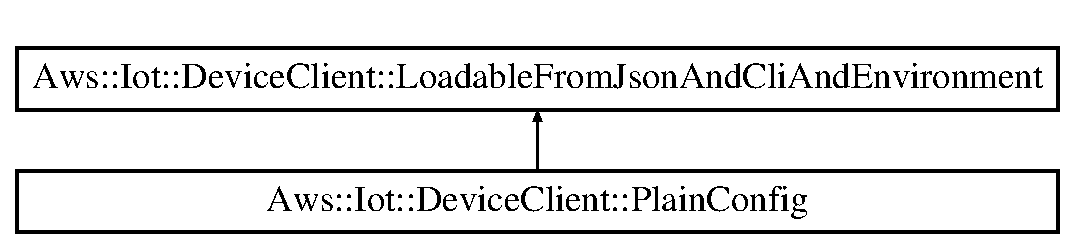
\includegraphics[height=2.000000cm]{struct_aws_1_1_iot_1_1_device_client_1_1_plain_config}
\end{center}
\end{figure}
\subsection*{Classes}
\begin{DoxyCompactItemize}
\item 
struct \hyperlink{struct_aws_1_1_iot_1_1_device_client_1_1_plain_config_1_1_device_defender}{Device\+Defender}
\item 
struct \hyperlink{struct_aws_1_1_iot_1_1_device_client_1_1_plain_config_1_1_fleet_provisioning}{Fleet\+Provisioning}
\item 
struct \hyperlink{struct_aws_1_1_iot_1_1_device_client_1_1_plain_config_1_1_fleet_provisioning_runtime_config}{Fleet\+Provisioning\+Runtime\+Config}
\item 
struct \hyperlink{struct_aws_1_1_iot_1_1_device_client_1_1_plain_config_1_1_jobs}{Jobs}
\item 
struct \hyperlink{struct_aws_1_1_iot_1_1_device_client_1_1_plain_config_1_1_log_config}{Log\+Config}
\item 
struct \hyperlink{struct_aws_1_1_iot_1_1_device_client_1_1_plain_config_1_1_tunneling}{Tunneling}
\end{DoxyCompactItemize}
\subsection*{Public Member Functions}
\begin{DoxyCompactItemize}
\item 
\mbox{\Hypertarget{struct_aws_1_1_iot_1_1_device_client_1_1_plain_config_a2cccd6d88d19ab4d15014fd718cb90fb}\label{struct_aws_1_1_iot_1_1_device_client_1_1_plain_config_a2cccd6d88d19ab4d15014fd718cb90fb}} 
bool {\bfseries Load\+From\+Json} (const Crt\+::\+Json\+View \&json) override
\item 
\mbox{\Hypertarget{struct_aws_1_1_iot_1_1_device_client_1_1_plain_config_aca2e22c920f0474f7be0fcb6bab1b44f}\label{struct_aws_1_1_iot_1_1_device_client_1_1_plain_config_aca2e22c920f0474f7be0fcb6bab1b44f}} 
bool {\bfseries Load\+From\+Cli\+Args} (const Cli\+Args \&cli\+Args) override
\item 
\mbox{\Hypertarget{struct_aws_1_1_iot_1_1_device_client_1_1_plain_config_abf75909bc58d9b0c6a0ca6fdd4ecbf60}\label{struct_aws_1_1_iot_1_1_device_client_1_1_plain_config_abf75909bc58d9b0c6a0ca6fdd4ecbf60}} 
bool {\bfseries Load\+From\+Environment} () override
\item 
\mbox{\Hypertarget{struct_aws_1_1_iot_1_1_device_client_1_1_plain_config_ae460d8fd7839cfb6992a984b6f96f784}\label{struct_aws_1_1_iot_1_1_device_client_1_1_plain_config_ae460d8fd7839cfb6992a984b6f96f784}} 
bool {\bfseries Validate} () const override
\end{DoxyCompactItemize}
\subsection*{Public Attributes}
\begin{DoxyCompactItemize}
\item 
\mbox{\Hypertarget{struct_aws_1_1_iot_1_1_device_client_1_1_plain_config_a8df03f69932e310308d17ba3a5039a6a}\label{struct_aws_1_1_iot_1_1_device_client_1_1_plain_config_a8df03f69932e310308d17ba3a5039a6a}} 
Aws\+::\+Crt\+::\+Optional$<$ std\+::string $>$ {\bfseries endpoint}
\item 
\mbox{\Hypertarget{struct_aws_1_1_iot_1_1_device_client_1_1_plain_config_a4bc8217423b75ca62110da9c3b143ca0}\label{struct_aws_1_1_iot_1_1_device_client_1_1_plain_config_a4bc8217423b75ca62110da9c3b143ca0}} 
Aws\+::\+Crt\+::\+Optional$<$ std\+::string $>$ {\bfseries cert}
\item 
\mbox{\Hypertarget{struct_aws_1_1_iot_1_1_device_client_1_1_plain_config_abfbb20a5277d201b3bfb423452fcd25f}\label{struct_aws_1_1_iot_1_1_device_client_1_1_plain_config_abfbb20a5277d201b3bfb423452fcd25f}} 
Aws\+::\+Crt\+::\+Optional$<$ std\+::string $>$ {\bfseries key}
\item 
\mbox{\Hypertarget{struct_aws_1_1_iot_1_1_device_client_1_1_plain_config_a76c14bcf8e605013362e48c34ded4170}\label{struct_aws_1_1_iot_1_1_device_client_1_1_plain_config_a76c14bcf8e605013362e48c34ded4170}} 
Aws\+::\+Crt\+::\+Optional$<$ std\+::string $>$ {\bfseries root\+Ca}
\item 
\mbox{\Hypertarget{struct_aws_1_1_iot_1_1_device_client_1_1_plain_config_abb8e33acedadfc1d646cc8df09bfda92}\label{struct_aws_1_1_iot_1_1_device_client_1_1_plain_config_abb8e33acedadfc1d646cc8df09bfda92}} 
Aws\+::\+Crt\+::\+Optional$<$ std\+::string $>$ {\bfseries thing\+Name}
\item 
\mbox{\Hypertarget{struct_aws_1_1_iot_1_1_device_client_1_1_plain_config_a11803ad7ce3316b92cd978c3f0ddc4fc}\label{struct_aws_1_1_iot_1_1_device_client_1_1_plain_config_a11803ad7ce3316b92cd978c3f0ddc4fc}} 
\hyperlink{struct_aws_1_1_iot_1_1_device_client_1_1_plain_config_1_1_log_config}{Log\+Config} {\bfseries log\+Config}
\item 
\mbox{\Hypertarget{struct_aws_1_1_iot_1_1_device_client_1_1_plain_config_a54fe51e92b940e3e98702c091c34a975}\label{struct_aws_1_1_iot_1_1_device_client_1_1_plain_config_a54fe51e92b940e3e98702c091c34a975}} 
\hyperlink{struct_aws_1_1_iot_1_1_device_client_1_1_plain_config_1_1_jobs}{Jobs} {\bfseries jobs}
\item 
\mbox{\Hypertarget{struct_aws_1_1_iot_1_1_device_client_1_1_plain_config_a32a8ac182f54498b383ffd2fe943b644}\label{struct_aws_1_1_iot_1_1_device_client_1_1_plain_config_a32a8ac182f54498b383ffd2fe943b644}} 
\hyperlink{struct_aws_1_1_iot_1_1_device_client_1_1_plain_config_1_1_tunneling}{Tunneling} {\bfseries tunneling}
\item 
\mbox{\Hypertarget{struct_aws_1_1_iot_1_1_device_client_1_1_plain_config_abf82b3c2d0e97cef5ab068872b1fd7d8}\label{struct_aws_1_1_iot_1_1_device_client_1_1_plain_config_abf82b3c2d0e97cef5ab068872b1fd7d8}} 
\hyperlink{struct_aws_1_1_iot_1_1_device_client_1_1_plain_config_1_1_device_defender}{Device\+Defender} {\bfseries device\+Defender}
\item 
\mbox{\Hypertarget{struct_aws_1_1_iot_1_1_device_client_1_1_plain_config_a536772112f9aa00380c77e18727debe2}\label{struct_aws_1_1_iot_1_1_device_client_1_1_plain_config_a536772112f9aa00380c77e18727debe2}} 
\hyperlink{struct_aws_1_1_iot_1_1_device_client_1_1_plain_config_1_1_fleet_provisioning}{Fleet\+Provisioning} {\bfseries fleet\+Provisioning}
\item 
\mbox{\Hypertarget{struct_aws_1_1_iot_1_1_device_client_1_1_plain_config_aa88bc09e13adc58d297ec82e1facd8dd}\label{struct_aws_1_1_iot_1_1_device_client_1_1_plain_config_aa88bc09e13adc58d297ec82e1facd8dd}} 
\hyperlink{struct_aws_1_1_iot_1_1_device_client_1_1_plain_config_1_1_fleet_provisioning_runtime_config}{Fleet\+Provisioning\+Runtime\+Config} {\bfseries fleet\+Provisioning\+Runtime\+Config}
\end{DoxyCompactItemize}
\subsection*{Static Public Attributes}
\begin{DoxyCompactItemize}
\item 
\mbox{\Hypertarget{struct_aws_1_1_iot_1_1_device_client_1_1_plain_config_a83c8d156e249b6b76f07c2948471f106}\label{struct_aws_1_1_iot_1_1_device_client_1_1_plain_config_a83c8d156e249b6b76f07c2948471f106}} 
static constexpr char {\bfseries C\+L\+I\+\_\+\+E\+N\+D\+P\+O\+I\+NT} \mbox{[}$\,$\mbox{]} = \char`\"{}-\/-\/endpoint\char`\"{}
\item 
\mbox{\Hypertarget{struct_aws_1_1_iot_1_1_device_client_1_1_plain_config_a39d731432687c04e6a11599cae19ab80}\label{struct_aws_1_1_iot_1_1_device_client_1_1_plain_config_a39d731432687c04e6a11599cae19ab80}} 
static constexpr char {\bfseries C\+L\+I\+\_\+\+C\+E\+RT} \mbox{[}$\,$\mbox{]} = \char`\"{}-\/-\/cert\char`\"{}
\item 
\mbox{\Hypertarget{struct_aws_1_1_iot_1_1_device_client_1_1_plain_config_a09987189e505b253c056c98b1702f772}\label{struct_aws_1_1_iot_1_1_device_client_1_1_plain_config_a09987189e505b253c056c98b1702f772}} 
static constexpr char {\bfseries C\+L\+I\+\_\+\+K\+EY} \mbox{[}$\,$\mbox{]} = \char`\"{}-\/-\/key\char`\"{}
\item 
\mbox{\Hypertarget{struct_aws_1_1_iot_1_1_device_client_1_1_plain_config_abff94c48ef664a9a40e67e0a7aa375fc}\label{struct_aws_1_1_iot_1_1_device_client_1_1_plain_config_abff94c48ef664a9a40e67e0a7aa375fc}} 
static constexpr char {\bfseries C\+L\+I\+\_\+\+R\+O\+O\+T\+\_\+\+CA} \mbox{[}$\,$\mbox{]} = \char`\"{}-\/-\/root-\/ca\char`\"{}
\item 
\mbox{\Hypertarget{struct_aws_1_1_iot_1_1_device_client_1_1_plain_config_a882b28082e2c4cfb8c49de8396a71fc9}\label{struct_aws_1_1_iot_1_1_device_client_1_1_plain_config_a882b28082e2c4cfb8c49de8396a71fc9}} 
static constexpr char {\bfseries C\+L\+I\+\_\+\+T\+H\+I\+N\+G\+\_\+\+N\+A\+ME} \mbox{[}$\,$\mbox{]} = \char`\"{}-\/-\/thing-\/name\char`\"{}
\item 
\mbox{\Hypertarget{struct_aws_1_1_iot_1_1_device_client_1_1_plain_config_ad1a0c4f00c566ae459c6af1bf721d6eb}\label{struct_aws_1_1_iot_1_1_device_client_1_1_plain_config_ad1a0c4f00c566ae459c6af1bf721d6eb}} 
static constexpr char {\bfseries J\+S\+O\+N\+\_\+\+K\+E\+Y\+\_\+\+E\+N\+D\+P\+O\+I\+NT} \mbox{[}$\,$\mbox{]} = \char`\"{}endpoint\char`\"{}
\item 
\mbox{\Hypertarget{struct_aws_1_1_iot_1_1_device_client_1_1_plain_config_a151ec4f604e170e6e544366e085159eb}\label{struct_aws_1_1_iot_1_1_device_client_1_1_plain_config_a151ec4f604e170e6e544366e085159eb}} 
static constexpr char {\bfseries J\+S\+O\+N\+\_\+\+K\+E\+Y\+\_\+\+C\+E\+RT} \mbox{[}$\,$\mbox{]} = \char`\"{}cert\char`\"{}
\item 
\mbox{\Hypertarget{struct_aws_1_1_iot_1_1_device_client_1_1_plain_config_a819fc8b7c4bfb3f508d6bf5d75e9a6c1}\label{struct_aws_1_1_iot_1_1_device_client_1_1_plain_config_a819fc8b7c4bfb3f508d6bf5d75e9a6c1}} 
static constexpr char {\bfseries J\+S\+O\+N\+\_\+\+K\+E\+Y\+\_\+\+K\+EY} \mbox{[}$\,$\mbox{]} = \char`\"{}key\char`\"{}
\item 
\mbox{\Hypertarget{struct_aws_1_1_iot_1_1_device_client_1_1_plain_config_a3295893aa8b4352533218adcc8cf3551}\label{struct_aws_1_1_iot_1_1_device_client_1_1_plain_config_a3295893aa8b4352533218adcc8cf3551}} 
static constexpr char {\bfseries J\+S\+O\+N\+\_\+\+K\+E\+Y\+\_\+\+R\+O\+O\+T\+\_\+\+CA} \mbox{[}$\,$\mbox{]} = \char`\"{}root-\/ca\char`\"{}
\item 
\mbox{\Hypertarget{struct_aws_1_1_iot_1_1_device_client_1_1_plain_config_a4e4874fe442e81ad007f0279b300ca6b}\label{struct_aws_1_1_iot_1_1_device_client_1_1_plain_config_a4e4874fe442e81ad007f0279b300ca6b}} 
static constexpr char {\bfseries J\+S\+O\+N\+\_\+\+K\+E\+Y\+\_\+\+T\+H\+I\+N\+G\+\_\+\+N\+A\+ME} \mbox{[}$\,$\mbox{]} = \char`\"{}thing-\/name\char`\"{}
\item 
\mbox{\Hypertarget{struct_aws_1_1_iot_1_1_device_client_1_1_plain_config_aaf9e46cfbf5aaf6e454ebc327f0dd8cc}\label{struct_aws_1_1_iot_1_1_device_client_1_1_plain_config_aaf9e46cfbf5aaf6e454ebc327f0dd8cc}} 
static constexpr char {\bfseries J\+S\+O\+N\+\_\+\+K\+E\+Y\+\_\+\+J\+O\+BS} \mbox{[}$\,$\mbox{]} = \char`\"{}jobs\char`\"{}
\item 
\mbox{\Hypertarget{struct_aws_1_1_iot_1_1_device_client_1_1_plain_config_a21479da245b17910d6694edede156bdf}\label{struct_aws_1_1_iot_1_1_device_client_1_1_plain_config_a21479da245b17910d6694edede156bdf}} 
static constexpr char {\bfseries J\+S\+O\+N\+\_\+\+K\+E\+Y\+\_\+\+T\+U\+N\+N\+E\+L\+I\+NG} \mbox{[}$\,$\mbox{]} = \char`\"{}tunneling\char`\"{}
\item 
\mbox{\Hypertarget{struct_aws_1_1_iot_1_1_device_client_1_1_plain_config_a788eadb68d1d226d01e38406f747dcd8}\label{struct_aws_1_1_iot_1_1_device_client_1_1_plain_config_a788eadb68d1d226d01e38406f747dcd8}} 
static constexpr char {\bfseries J\+S\+O\+N\+\_\+\+K\+E\+Y\+\_\+\+D\+E\+V\+I\+C\+E\+\_\+\+D\+E\+F\+E\+N\+D\+ER} \mbox{[}$\,$\mbox{]} = \char`\"{}device-\/defender\char`\"{}
\item 
\mbox{\Hypertarget{struct_aws_1_1_iot_1_1_device_client_1_1_plain_config_a23f968f89365ab975f6c846450d52f2d}\label{struct_aws_1_1_iot_1_1_device_client_1_1_plain_config_a23f968f89365ab975f6c846450d52f2d}} 
static constexpr char {\bfseries J\+S\+O\+N\+\_\+\+K\+E\+Y\+\_\+\+F\+L\+E\+E\+T\+\_\+\+P\+R\+O\+V\+I\+S\+I\+O\+N\+I\+NG} \mbox{[}$\,$\mbox{]} = \char`\"{}fleet-\/provisioning\char`\"{}
\item 
\mbox{\Hypertarget{struct_aws_1_1_iot_1_1_device_client_1_1_plain_config_a835132c6f3880fad1b2f5677c0dc7c01}\label{struct_aws_1_1_iot_1_1_device_client_1_1_plain_config_a835132c6f3880fad1b2f5677c0dc7c01}} 
static constexpr char {\bfseries J\+S\+O\+N\+\_\+\+K\+E\+Y\+\_\+\+R\+U\+N\+T\+I\+M\+E\+\_\+\+C\+O\+N\+F\+IG} \mbox{[}$\,$\mbox{]} = \char`\"{}runtime-\/config\char`\"{}
\item 
\mbox{\Hypertarget{struct_aws_1_1_iot_1_1_device_client_1_1_plain_config_adde6d544fcec7cc47356908c751b6d16}\label{struct_aws_1_1_iot_1_1_device_client_1_1_plain_config_adde6d544fcec7cc47356908c751b6d16}} 
static constexpr char {\bfseries J\+S\+O\+N\+\_\+\+K\+E\+Y\+\_\+\+L\+O\+G\+G\+I\+NG} \mbox{[}$\,$\mbox{]} = \char`\"{}logging\char`\"{}
\end{DoxyCompactItemize}


The documentation for this struct was generated from the following files\+:\begin{DoxyCompactItemize}
\item 
/home/\+A\+N\+T.\+A\+M\+A\+Z\+O\+N.\+C\+O\+M/lwwilkov/\+Workspace/aws-\/iot-\/device-\/client/source/config/Config.\+h\item 
/home/\+A\+N\+T.\+A\+M\+A\+Z\+O\+N.\+C\+O\+M/lwwilkov/\+Workspace/aws-\/iot-\/device-\/client/source/config/Config.\+cpp\end{DoxyCompactItemize}

\hypertarget{class_aws_1_1_iot_1_1_device_client_1_1_util_1_1_retry}{}\section{Aws\+:\+:Iot\+:\+:Device\+Client\+:\+:Util\+:\+:Retry Class Reference}
\label{class_aws_1_1_iot_1_1_device_client_1_1_util_1_1_retry}\index{Aws\+::\+Iot\+::\+Device\+Client\+::\+Util\+::\+Retry@{Aws\+::\+Iot\+::\+Device\+Client\+::\+Util\+::\+Retry}}


Provides utility methods for retrying a function.  




{\ttfamily \#include $<$Retry.\+h$>$}

\subsection*{Classes}
\begin{DoxyCompactItemize}
\item 
struct \hyperlink{struct_aws_1_1_iot_1_1_device_client_1_1_util_1_1_retry_1_1_exponential_retry_config}{Exponential\+Retry\+Config}
\begin{DoxyCompactList}\small\item\em Used for passing an exponential retry configuration to the exponential\+Backoff function. \end{DoxyCompactList}\end{DoxyCompactItemize}
\subsection*{Static Public Member Functions}
\begin{DoxyCompactItemize}
\item 
static bool \hyperlink{class_aws_1_1_iot_1_1_device_client_1_1_util_1_1_retry_a6d55342ef0ae5d2a10e40b317e9c51cc}{exponential\+Backoff} (std\+::function$<$ bool()$>$ retryable\+Function, \hyperlink{struct_aws_1_1_iot_1_1_device_client_1_1_util_1_1_retry_1_1_exponential_retry_config}{Exponential\+Retry\+Config} config)
\begin{DoxyCompactList}\small\item\em Performs an exponential backoff of the provided function based on the specified \hyperlink{struct_aws_1_1_iot_1_1_device_client_1_1_util_1_1_retry_1_1_exponential_retry_config}{Exponential\+Retry\+Config}. \end{DoxyCompactList}\end{DoxyCompactItemize}
\subsection*{Static Private Attributes}
\begin{DoxyCompactItemize}
\item 
\mbox{\Hypertarget{class_aws_1_1_iot_1_1_device_client_1_1_util_1_1_retry_a089016a730bb3f65c6173a1fe7f34116}\label{class_aws_1_1_iot_1_1_device_client_1_1_util_1_1_retry_a089016a730bb3f65c6173a1fe7f34116}} 
static const char $\ast$ {\bfseries T\+AG} = \char`\"{}Retry.\+cpp\char`\"{}
\end{DoxyCompactItemize}


\subsection{Detailed Description}
Provides utility methods for retrying a function. 

\subsection{Member Function Documentation}
\mbox{\Hypertarget{class_aws_1_1_iot_1_1_device_client_1_1_util_1_1_retry_a6d55342ef0ae5d2a10e40b317e9c51cc}\label{class_aws_1_1_iot_1_1_device_client_1_1_util_1_1_retry_a6d55342ef0ae5d2a10e40b317e9c51cc}} 
\index{Aws\+::\+Iot\+::\+Device\+Client\+::\+Util\+::\+Retry@{Aws\+::\+Iot\+::\+Device\+Client\+::\+Util\+::\+Retry}!exponential\+Backoff@{exponential\+Backoff}}
\index{exponential\+Backoff@{exponential\+Backoff}!Aws\+::\+Iot\+::\+Device\+Client\+::\+Util\+::\+Retry@{Aws\+::\+Iot\+::\+Device\+Client\+::\+Util\+::\+Retry}}
\subsubsection{\texorpdfstring{exponential\+Backoff()}{exponentialBackoff()}}
{\footnotesize\ttfamily bool Retry\+::exponential\+Backoff (\begin{DoxyParamCaption}\item[{std\+::function$<$ bool()$>$}]{retryable\+Function,  }\item[{\hyperlink{struct_aws_1_1_iot_1_1_device_client_1_1_util_1_1_retry_1_1_exponential_retry_config}{Exponential\+Retry\+Config}}]{config }\end{DoxyParamCaption})\hspace{0.3cm}{\ttfamily [static]}}



Performs an exponential backoff of the provided function based on the specified \hyperlink{struct_aws_1_1_iot_1_1_device_client_1_1_util_1_1_retry_1_1_exponential_retry_config}{Exponential\+Retry\+Config}. 

In the event of throttling by IoT Core A\+P\+Is, such as when we perform Update\+Job\+Execution within the Jobs feature, it is necessary to perform an exponential backoff to improve the chances of receiving a success response. 
\begin{DoxyParams}{Parameters}
{\em retryable\+Function} & the function to retry. This function should return a bool indicating whether it is successful or not, since this indicator is what will determine whether the function is retried or not. \\
\hline
{\em config} & the \hyperlink{struct_aws_1_1_iot_1_1_device_client_1_1_util_1_1_retry_1_1_exponential_retry_config}{Exponential\+Retry\+Config} specifying whether the function should be retried \\
\hline
\end{DoxyParams}
\begin{DoxyReturn}{Returns}
a bool representing whether the retryable\+Function was successful or not 
\end{DoxyReturn}


The documentation for this class was generated from the following files\+:\begin{DoxyCompactItemize}
\item 
/home/\+A\+N\+T.\+A\+M\+A\+Z\+O\+N.\+C\+O\+M/lwwilkov/\+Workspace/aws-\/iot-\/device-\/client/source/util/Retry.\+h\item 
/home/\+A\+N\+T.\+A\+M\+A\+Z\+O\+N.\+C\+O\+M/lwwilkov/\+Workspace/aws-\/iot-\/device-\/client/source/util/Retry.\+cpp\end{DoxyCompactItemize}

\hypertarget{class_aws_1_1_iot_1_1_device_client_1_1_secure_tunneling_1_1_secure_tunneling_context}{}\section{Aws\+:\+:Iot\+:\+:Device\+Client\+:\+:Secure\+Tunneling\+:\+:Secure\+Tunneling\+Context Class Reference}
\label{class_aws_1_1_iot_1_1_device_client_1_1_secure_tunneling_1_1_secure_tunneling_context}\index{Aws\+::\+Iot\+::\+Device\+Client\+::\+Secure\+Tunneling\+::\+Secure\+Tunneling\+Context@{Aws\+::\+Iot\+::\+Device\+Client\+::\+Secure\+Tunneling\+::\+Secure\+Tunneling\+Context}}


A class that represents a secure tunnel and local T\+CP port forward pair. The class also implements all the callbacks required for secure tunneling and local T\+CP port forward.  




{\ttfamily \#include $<$Secure\+Tunneling\+Context.\+h$>$}

\subsection*{Public Member Functions}
\begin{DoxyCompactItemize}
\item 
\hyperlink{class_aws_1_1_iot_1_1_device_client_1_1_secure_tunneling_1_1_secure_tunneling_context_a7619ca8a373c28c33a59615f69d6a2fc}{Secure\+Tunneling\+Context} (std\+::shared\+\_\+ptr$<$ \hyperlink{class_aws_1_1_iot_1_1_device_client_1_1_shared_crt_resource_manager}{Shared\+Crt\+Resource\+Manager} $>$ manager, const std\+::string \&root\+Ca, const std\+::string \&access\+Token, const std\+::string \&endpoint, uint16\+\_\+t port, On\+Connection\+Shutdown\+Fn on\+Connection\+Shutdown)
\begin{DoxyCompactList}\small\item\em Constructor. \end{DoxyCompactList}\item 
\mbox{\Hypertarget{class_aws_1_1_iot_1_1_device_client_1_1_secure_tunneling_1_1_secure_tunneling_context_aa416f61064dda593184cedd86e16acbe}\label{class_aws_1_1_iot_1_1_device_client_1_1_secure_tunneling_1_1_secure_tunneling_context_aa416f61064dda593184cedd86e16acbe}} 
\hyperlink{class_aws_1_1_iot_1_1_device_client_1_1_secure_tunneling_1_1_secure_tunneling_context_aa416f61064dda593184cedd86e16acbe}{$\sim$\+Secure\+Tunneling\+Context} ()
\begin{DoxyCompactList}\small\item\em Destructor. \end{DoxyCompactList}\item 
bool \hyperlink{class_aws_1_1_iot_1_1_device_client_1_1_secure_tunneling_1_1_secure_tunneling_context_a2903abce816d29356985d7a37cde728e}{Is\+Duplicate\+Notification} (const Aws\+::\+Iotsecuretunneling\+::\+Secure\+Tunneling\+Notify\+Response \&response)
\begin{DoxyCompactList}\small\item\em Check to see if we have seen and processed the given M\+Q\+TT notification. \end{DoxyCompactList}\item 
bool \hyperlink{class_aws_1_1_iot_1_1_device_client_1_1_secure_tunneling_1_1_secure_tunneling_context_a521c773c7019dc456922500627d241e8}{Connect\+To\+Secure\+Tunnel} ()
\begin{DoxyCompactList}\small\item\em Connect to a secure tunnel. \end{DoxyCompactList}\end{DoxyCompactItemize}
\subsection*{Private Member Functions}
\begin{DoxyCompactItemize}
\item 
\mbox{\Hypertarget{class_aws_1_1_iot_1_1_device_client_1_1_secure_tunneling_1_1_secure_tunneling_context_a52c98c3f5cb3e81e8dabbc35dbf19f76}\label{class_aws_1_1_iot_1_1_device_client_1_1_secure_tunneling_1_1_secure_tunneling_context_a52c98c3f5cb3e81e8dabbc35dbf19f76}} 
void \hyperlink{class_aws_1_1_iot_1_1_device_client_1_1_secure_tunneling_1_1_secure_tunneling_context_a52c98c3f5cb3e81e8dabbc35dbf19f76}{Connect\+To\+Tcp\+Forward} ()
\begin{DoxyCompactList}\small\item\em Connect to local T\+CP forward. \end{DoxyCompactList}\item 
\mbox{\Hypertarget{class_aws_1_1_iot_1_1_device_client_1_1_secure_tunneling_1_1_secure_tunneling_context_ad97af549a42effe5815a34e95a18ec24}\label{class_aws_1_1_iot_1_1_device_client_1_1_secure_tunneling_1_1_secure_tunneling_context_ad97af549a42effe5815a34e95a18ec24}} 
void \hyperlink{class_aws_1_1_iot_1_1_device_client_1_1_secure_tunneling_1_1_secure_tunneling_context_ad97af549a42effe5815a34e95a18ec24}{Disconnect\+From\+Tcp\+Forward} ()
\begin{DoxyCompactList}\small\item\em Disconnect from local T\+CP forward. \end{DoxyCompactList}\item 
\mbox{\Hypertarget{class_aws_1_1_iot_1_1_device_client_1_1_secure_tunneling_1_1_secure_tunneling_context_a394e303d5f6111f8ad94c040bfd35be9}\label{class_aws_1_1_iot_1_1_device_client_1_1_secure_tunneling_1_1_secure_tunneling_context_a394e303d5f6111f8ad94c040bfd35be9}} 
void \hyperlink{class_aws_1_1_iot_1_1_device_client_1_1_secure_tunneling_1_1_secure_tunneling_context_a394e303d5f6111f8ad94c040bfd35be9}{On\+Connection\+Complete} ()
\begin{DoxyCompactList}\small\item\em Callback when secure tunnel connection is complete. \end{DoxyCompactList}\item 
\mbox{\Hypertarget{class_aws_1_1_iot_1_1_device_client_1_1_secure_tunneling_1_1_secure_tunneling_context_a5b1f07f8a5b26e4f698430589ce4b6c4}\label{class_aws_1_1_iot_1_1_device_client_1_1_secure_tunneling_1_1_secure_tunneling_context_a5b1f07f8a5b26e4f698430589ce4b6c4}} 
void \hyperlink{class_aws_1_1_iot_1_1_device_client_1_1_secure_tunneling_1_1_secure_tunneling_context_a5b1f07f8a5b26e4f698430589ce4b6c4}{On\+Connection\+Shutdown} ()
\begin{DoxyCompactList}\small\item\em Callback when secure tunnel connection is shutdown. \end{DoxyCompactList}\item 
void \hyperlink{class_aws_1_1_iot_1_1_device_client_1_1_secure_tunneling_1_1_secure_tunneling_context_ae65a8bbb27479f1310a708f354c35b9d}{On\+Send\+Data\+Complete} (int error\+Code)
\begin{DoxyCompactList}\small\item\em Callback when data send to secure tunnel is complete. \end{DoxyCompactList}\item 
void \hyperlink{class_aws_1_1_iot_1_1_device_client_1_1_secure_tunneling_1_1_secure_tunneling_context_a778a6fd8e30ec1c14d4b57443acdb5ac}{On\+Data\+Receive} (const Crt\+::\+Byte\+Buf \&data)
\begin{DoxyCompactList}\small\item\em Callback when data is received from secure tunnel. \end{DoxyCompactList}\item 
\mbox{\Hypertarget{class_aws_1_1_iot_1_1_device_client_1_1_secure_tunneling_1_1_secure_tunneling_context_a35943770e783bc406b867dc951c107a2}\label{class_aws_1_1_iot_1_1_device_client_1_1_secure_tunneling_1_1_secure_tunneling_context_a35943770e783bc406b867dc951c107a2}} 
void \hyperlink{class_aws_1_1_iot_1_1_device_client_1_1_secure_tunneling_1_1_secure_tunneling_context_a35943770e783bc406b867dc951c107a2}{On\+Stream\+Start} ()
\begin{DoxyCompactList}\small\item\em Callback when secure tunnel stream\+\_\+start is received. \end{DoxyCompactList}\item 
\mbox{\Hypertarget{class_aws_1_1_iot_1_1_device_client_1_1_secure_tunneling_1_1_secure_tunneling_context_a3900c7ed3eeaa110d440d3b7763c07ac}\label{class_aws_1_1_iot_1_1_device_client_1_1_secure_tunneling_1_1_secure_tunneling_context_a3900c7ed3eeaa110d440d3b7763c07ac}} 
void \hyperlink{class_aws_1_1_iot_1_1_device_client_1_1_secure_tunneling_1_1_secure_tunneling_context_a3900c7ed3eeaa110d440d3b7763c07ac}{On\+Stream\+Reset} ()
\begin{DoxyCompactList}\small\item\em Callback when secure tunnel stream\+\_\+reset is received. \end{DoxyCompactList}\item 
\mbox{\Hypertarget{class_aws_1_1_iot_1_1_device_client_1_1_secure_tunneling_1_1_secure_tunneling_context_a3863d150eee150129127e0639286907d}\label{class_aws_1_1_iot_1_1_device_client_1_1_secure_tunneling_1_1_secure_tunneling_context_a3863d150eee150129127e0639286907d}} 
void \hyperlink{class_aws_1_1_iot_1_1_device_client_1_1_secure_tunneling_1_1_secure_tunneling_context_a3863d150eee150129127e0639286907d}{On\+Session\+Reset} ()
\begin{DoxyCompactList}\small\item\em Callback when secure tunnel session\+\_\+reset is received. \end{DoxyCompactList}\item 
void \hyperlink{class_aws_1_1_iot_1_1_device_client_1_1_secure_tunneling_1_1_secure_tunneling_context_a72d579a67fd19f1462a15cee8033de73}{On\+Tcp\+Forward\+Data\+Receive} (const Crt\+::\+Byte\+Buf \&data)
\begin{DoxyCompactList}\small\item\em Callback when data is received from the local T\+CP port. \end{DoxyCompactList}\end{DoxyCompactItemize}
\subsection*{Private Attributes}
\begin{DoxyCompactItemize}
\item 
\mbox{\Hypertarget{class_aws_1_1_iot_1_1_device_client_1_1_secure_tunneling_1_1_secure_tunneling_context_a7b2b3ec32fadb243eefdf40f55c9dcbf}\label{class_aws_1_1_iot_1_1_device_client_1_1_secure_tunneling_1_1_secure_tunneling_context_a7b2b3ec32fadb243eefdf40f55c9dcbf}} 
std\+::shared\+\_\+ptr$<$ \hyperlink{class_aws_1_1_iot_1_1_device_client_1_1_shared_crt_resource_manager}{Shared\+Crt\+Resource\+Manager} $>$ \hyperlink{class_aws_1_1_iot_1_1_device_client_1_1_secure_tunneling_1_1_secure_tunneling_context_a7b2b3ec32fadb243eefdf40f55c9dcbf}{m\+Shared\+Crt\+Resource\+Manager}
\begin{DoxyCompactList}\small\item\em The resource manager used to manage C\+RT resources. \end{DoxyCompactList}\item 
\mbox{\Hypertarget{class_aws_1_1_iot_1_1_device_client_1_1_secure_tunneling_1_1_secure_tunneling_context_abe29a269fb28c92b4703ac2ca7e585af}\label{class_aws_1_1_iot_1_1_device_client_1_1_secure_tunneling_1_1_secure_tunneling_context_abe29a269fb28c92b4703ac2ca7e585af}} 
std\+::string \hyperlink{class_aws_1_1_iot_1_1_device_client_1_1_secure_tunneling_1_1_secure_tunneling_context_abe29a269fb28c92b4703ac2ca7e585af}{m\+Root\+Ca}
\begin{DoxyCompactList}\small\item\em Path to the Amazon root CA. \end{DoxyCompactList}\item 
\mbox{\Hypertarget{class_aws_1_1_iot_1_1_device_client_1_1_secure_tunneling_1_1_secure_tunneling_context_a6fddc24c6add770d088741a75f0ea91f}\label{class_aws_1_1_iot_1_1_device_client_1_1_secure_tunneling_1_1_secure_tunneling_context_a6fddc24c6add770d088741a75f0ea91f}} 
std\+::string \hyperlink{class_aws_1_1_iot_1_1_device_client_1_1_secure_tunneling_1_1_secure_tunneling_context_a6fddc24c6add770d088741a75f0ea91f}{m\+Access\+Token}
\begin{DoxyCompactList}\small\item\em Destination access token. \end{DoxyCompactList}\item 
\mbox{\Hypertarget{class_aws_1_1_iot_1_1_device_client_1_1_secure_tunneling_1_1_secure_tunneling_context_aa07933f466bffedac5718eb90961691a}\label{class_aws_1_1_iot_1_1_device_client_1_1_secure_tunneling_1_1_secure_tunneling_context_aa07933f466bffedac5718eb90961691a}} 
std\+::string \hyperlink{class_aws_1_1_iot_1_1_device_client_1_1_secure_tunneling_1_1_secure_tunneling_context_aa07933f466bffedac5718eb90961691a}{m\+Endpoint}
\begin{DoxyCompactList}\small\item\em Secure Tunneling data plain endpoint. \end{DoxyCompactList}\item 
\mbox{\Hypertarget{class_aws_1_1_iot_1_1_device_client_1_1_secure_tunneling_1_1_secure_tunneling_context_ae87a537fedeb6aef41ba8f7352fc2a86}\label{class_aws_1_1_iot_1_1_device_client_1_1_secure_tunneling_1_1_secure_tunneling_context_ae87a537fedeb6aef41ba8f7352fc2a86}} 
uint16\+\_\+t \hyperlink{class_aws_1_1_iot_1_1_device_client_1_1_secure_tunneling_1_1_secure_tunneling_context_ae87a537fedeb6aef41ba8f7352fc2a86}{m\+Port} \{22\}
\begin{DoxyCompactList}\small\item\em The local T\+CP port to connect to. \end{DoxyCompactList}\item 
\mbox{\Hypertarget{class_aws_1_1_iot_1_1_device_client_1_1_secure_tunneling_1_1_secure_tunneling_context_a6e2f845575d6e01a4dcf11585b79948a}\label{class_aws_1_1_iot_1_1_device_client_1_1_secure_tunneling_1_1_secure_tunneling_context_a6e2f845575d6e01a4dcf11585b79948a}} 
On\+Connection\+Shutdown\+Fn \hyperlink{class_aws_1_1_iot_1_1_device_client_1_1_secure_tunneling_1_1_secure_tunneling_context_a6e2f845575d6e01a4dcf11585b79948a}{m\+On\+Connection\+Shutdown}
\begin{DoxyCompactList}\small\item\em Callback when the secure tunnel is shutdown. \end{DoxyCompactList}\item 
\mbox{\Hypertarget{class_aws_1_1_iot_1_1_device_client_1_1_secure_tunneling_1_1_secure_tunneling_context_a4f4a7c085ff9a1f4d1c4df317e986823}\label{class_aws_1_1_iot_1_1_device_client_1_1_secure_tunneling_1_1_secure_tunneling_context_a4f4a7c085ff9a1f4d1c4df317e986823}} 
std\+::unique\+\_\+ptr$<$ Aws\+::\+Iotsecuretunneling\+::\+Secure\+Tunnel $>$ \hyperlink{class_aws_1_1_iot_1_1_device_client_1_1_secure_tunneling_1_1_secure_tunneling_context_a4f4a7c085ff9a1f4d1c4df317e986823}{m\+Secure\+Tunnel}
\begin{DoxyCompactList}\small\item\em An A\+WS IoT S\+DK Secure Tunnel object. It manages the secure tunnel. \end{DoxyCompactList}\item 
\mbox{\Hypertarget{class_aws_1_1_iot_1_1_device_client_1_1_secure_tunneling_1_1_secure_tunneling_context_a340b87ef9235822ac609a9ff62cd698d}\label{class_aws_1_1_iot_1_1_device_client_1_1_secure_tunneling_1_1_secure_tunneling_context_a340b87ef9235822ac609a9ff62cd698d}} 
std\+::unique\+\_\+ptr$<$ \hyperlink{class_aws_1_1_iot_1_1_device_client_1_1_secure_tunneling_1_1_tcp_forward}{Tcp\+Forward} $>$ \hyperlink{class_aws_1_1_iot_1_1_device_client_1_1_secure_tunneling_1_1_secure_tunneling_context_a340b87ef9235822ac609a9ff62cd698d}{m\+Tcp\+Forward}
\begin{DoxyCompactList}\small\item\em Manages local T\+CP port forward. \end{DoxyCompactList}\item 
\mbox{\Hypertarget{class_aws_1_1_iot_1_1_device_client_1_1_secure_tunneling_1_1_secure_tunneling_context_abb811790d7df9ec7d079f0e99626e912}\label{class_aws_1_1_iot_1_1_device_client_1_1_secure_tunneling_1_1_secure_tunneling_context_abb811790d7df9ec7d079f0e99626e912}} 
Aws\+::\+Crt\+::\+Optional$<$ Aws\+::\+Iotsecuretunneling\+::\+Secure\+Tunneling\+Notify\+Response $>$ \hyperlink{class_aws_1_1_iot_1_1_device_client_1_1_secure_tunneling_1_1_secure_tunneling_context_abb811790d7df9ec7d079f0e99626e912}{m\+Last\+Seen\+Notify\+Response}
\begin{DoxyCompactList}\small\item\em Save the M\+Q\+TT new tunnel notification that results in the creation of this tunnel context. This is used to avoid creating duplicate tunnel contexts as A\+WS M\+Q\+TT Broker may send duplicate notifications. \end{DoxyCompactList}\end{DoxyCompactItemize}
\subsection*{Static Private Attributes}
\begin{DoxyCompactItemize}
\item 
\mbox{\Hypertarget{class_aws_1_1_iot_1_1_device_client_1_1_secure_tunneling_1_1_secure_tunneling_context_a28cc91d533330283781464efe5ce72c8}\label{class_aws_1_1_iot_1_1_device_client_1_1_secure_tunneling_1_1_secure_tunneling_context_a28cc91d533330283781464efe5ce72c8}} 
static constexpr char \hyperlink{class_aws_1_1_iot_1_1_device_client_1_1_secure_tunneling_1_1_secure_tunneling_context_a28cc91d533330283781464efe5ce72c8}{T\+AG} \mbox{[}$\,$\mbox{]} = \char`\"{}Secure\+Tunneling\+Context.\+cpp\char`\"{}
\begin{DoxyCompactList}\small\item\em Used by the logger to specify that log messages are coming from this class. \end{DoxyCompactList}\end{DoxyCompactItemize}


\subsection{Detailed Description}
A class that represents a secure tunnel and local T\+CP port forward pair. The class also implements all the callbacks required for secure tunneling and local T\+CP port forward. 

\subsection{Constructor \& Destructor Documentation}
\mbox{\Hypertarget{class_aws_1_1_iot_1_1_device_client_1_1_secure_tunneling_1_1_secure_tunneling_context_a7619ca8a373c28c33a59615f69d6a2fc}\label{class_aws_1_1_iot_1_1_device_client_1_1_secure_tunneling_1_1_secure_tunneling_context_a7619ca8a373c28c33a59615f69d6a2fc}} 
\index{Aws\+::\+Iot\+::\+Device\+Client\+::\+Secure\+Tunneling\+::\+Secure\+Tunneling\+Context@{Aws\+::\+Iot\+::\+Device\+Client\+::\+Secure\+Tunneling\+::\+Secure\+Tunneling\+Context}!Secure\+Tunneling\+Context@{Secure\+Tunneling\+Context}}
\index{Secure\+Tunneling\+Context@{Secure\+Tunneling\+Context}!Aws\+::\+Iot\+::\+Device\+Client\+::\+Secure\+Tunneling\+::\+Secure\+Tunneling\+Context@{Aws\+::\+Iot\+::\+Device\+Client\+::\+Secure\+Tunneling\+::\+Secure\+Tunneling\+Context}}
\subsubsection{\texorpdfstring{Secure\+Tunneling\+Context()}{SecureTunnelingContext()}}
{\footnotesize\ttfamily Aws\+::\+Iot\+::\+Device\+Client\+::\+Secure\+Tunneling\+::\+Secure\+Tunneling\+Context\+::\+Secure\+Tunneling\+Context (\begin{DoxyParamCaption}\item[{std\+::shared\+\_\+ptr$<$ \hyperlink{class_aws_1_1_iot_1_1_device_client_1_1_shared_crt_resource_manager}{Shared\+Crt\+Resource\+Manager} $>$}]{manager,  }\item[{const std\+::string \&}]{root\+Ca,  }\item[{const std\+::string \&}]{access\+Token,  }\item[{const std\+::string \&}]{endpoint,  }\item[{uint16\+\_\+t}]{port,  }\item[{On\+Connection\+Shutdown\+Fn}]{on\+Connection\+Shutdown }\end{DoxyParamCaption})}



Constructor. 


\begin{DoxyParams}{Parameters}
{\em manager} & the shared resource manager \\
\hline
{\em root\+Ca} & path to the Amazon root CA \\
\hline
{\em access\+Token} & destination access token for connecting to a secure tunnel \\
\hline
{\em endpoint} & secure tunneling data plain endpoint \\
\hline
{\em port} & the local T\+CP port to connect to \\
\hline
{\em on\+Connection\+Shutdown} & callback when the secure tunnel is shutdown \\
\hline
\end{DoxyParams}


\subsection{Member Function Documentation}
\mbox{\Hypertarget{class_aws_1_1_iot_1_1_device_client_1_1_secure_tunneling_1_1_secure_tunneling_context_a521c773c7019dc456922500627d241e8}\label{class_aws_1_1_iot_1_1_device_client_1_1_secure_tunneling_1_1_secure_tunneling_context_a521c773c7019dc456922500627d241e8}} 
\index{Aws\+::\+Iot\+::\+Device\+Client\+::\+Secure\+Tunneling\+::\+Secure\+Tunneling\+Context@{Aws\+::\+Iot\+::\+Device\+Client\+::\+Secure\+Tunneling\+::\+Secure\+Tunneling\+Context}!Connect\+To\+Secure\+Tunnel@{Connect\+To\+Secure\+Tunnel}}
\index{Connect\+To\+Secure\+Tunnel@{Connect\+To\+Secure\+Tunnel}!Aws\+::\+Iot\+::\+Device\+Client\+::\+Secure\+Tunneling\+::\+Secure\+Tunneling\+Context@{Aws\+::\+Iot\+::\+Device\+Client\+::\+Secure\+Tunneling\+::\+Secure\+Tunneling\+Context}}
\subsubsection{\texorpdfstring{Connect\+To\+Secure\+Tunnel()}{ConnectToSecureTunnel()}}
{\footnotesize\ttfamily bool Aws\+::\+Iot\+::\+Device\+Client\+::\+Secure\+Tunneling\+::\+Secure\+Tunneling\+Context\+::\+Connect\+To\+Secure\+Tunnel (\begin{DoxyParamCaption}{ }\end{DoxyParamCaption})}



Connect to a secure tunnel. 

\begin{DoxyReturn}{Returns}
True if successfully connected to the tunnel. False otherwise. 
\end{DoxyReturn}
\mbox{\Hypertarget{class_aws_1_1_iot_1_1_device_client_1_1_secure_tunneling_1_1_secure_tunneling_context_a2903abce816d29356985d7a37cde728e}\label{class_aws_1_1_iot_1_1_device_client_1_1_secure_tunneling_1_1_secure_tunneling_context_a2903abce816d29356985d7a37cde728e}} 
\index{Aws\+::\+Iot\+::\+Device\+Client\+::\+Secure\+Tunneling\+::\+Secure\+Tunneling\+Context@{Aws\+::\+Iot\+::\+Device\+Client\+::\+Secure\+Tunneling\+::\+Secure\+Tunneling\+Context}!Is\+Duplicate\+Notification@{Is\+Duplicate\+Notification}}
\index{Is\+Duplicate\+Notification@{Is\+Duplicate\+Notification}!Aws\+::\+Iot\+::\+Device\+Client\+::\+Secure\+Tunneling\+::\+Secure\+Tunneling\+Context@{Aws\+::\+Iot\+::\+Device\+Client\+::\+Secure\+Tunneling\+::\+Secure\+Tunneling\+Context}}
\subsubsection{\texorpdfstring{Is\+Duplicate\+Notification()}{IsDuplicateNotification()}}
{\footnotesize\ttfamily bool Aws\+::\+Iot\+::\+Device\+Client\+::\+Secure\+Tunneling\+::\+Secure\+Tunneling\+Context\+::\+Is\+Duplicate\+Notification (\begin{DoxyParamCaption}\item[{const Aws\+::\+Iotsecuretunneling\+::\+Secure\+Tunneling\+Notify\+Response \&}]{response }\end{DoxyParamCaption})}



Check to see if we have seen and processed the given M\+Q\+TT notification. 


\begin{DoxyParams}{Parameters}
{\em response} & M\+Q\+TT notification \\
\hline
\end{DoxyParams}
\begin{DoxyReturn}{Returns}
True if the given M\+Q\+TT notification is a duplication. False otherwise. 
\end{DoxyReturn}
\mbox{\Hypertarget{class_aws_1_1_iot_1_1_device_client_1_1_secure_tunneling_1_1_secure_tunneling_context_a778a6fd8e30ec1c14d4b57443acdb5ac}\label{class_aws_1_1_iot_1_1_device_client_1_1_secure_tunneling_1_1_secure_tunneling_context_a778a6fd8e30ec1c14d4b57443acdb5ac}} 
\index{Aws\+::\+Iot\+::\+Device\+Client\+::\+Secure\+Tunneling\+::\+Secure\+Tunneling\+Context@{Aws\+::\+Iot\+::\+Device\+Client\+::\+Secure\+Tunneling\+::\+Secure\+Tunneling\+Context}!On\+Data\+Receive@{On\+Data\+Receive}}
\index{On\+Data\+Receive@{On\+Data\+Receive}!Aws\+::\+Iot\+::\+Device\+Client\+::\+Secure\+Tunneling\+::\+Secure\+Tunneling\+Context@{Aws\+::\+Iot\+::\+Device\+Client\+::\+Secure\+Tunneling\+::\+Secure\+Tunneling\+Context}}
\subsubsection{\texorpdfstring{On\+Data\+Receive()}{OnDataReceive()}}
{\footnotesize\ttfamily void Aws\+::\+Iot\+::\+Device\+Client\+::\+Secure\+Tunneling\+::\+Secure\+Tunneling\+Context\+::\+On\+Data\+Receive (\begin{DoxyParamCaption}\item[{const Crt\+::\+Byte\+Buf \&}]{data }\end{DoxyParamCaption})\hspace{0.3cm}{\ttfamily [private]}}



Callback when data is received from secure tunnel. 


\begin{DoxyParams}{Parameters}
{\em data} & data received from the secure tunnel \\
\hline
\end{DoxyParams}
\mbox{\Hypertarget{class_aws_1_1_iot_1_1_device_client_1_1_secure_tunneling_1_1_secure_tunneling_context_ae65a8bbb27479f1310a708f354c35b9d}\label{class_aws_1_1_iot_1_1_device_client_1_1_secure_tunneling_1_1_secure_tunneling_context_ae65a8bbb27479f1310a708f354c35b9d}} 
\index{Aws\+::\+Iot\+::\+Device\+Client\+::\+Secure\+Tunneling\+::\+Secure\+Tunneling\+Context@{Aws\+::\+Iot\+::\+Device\+Client\+::\+Secure\+Tunneling\+::\+Secure\+Tunneling\+Context}!On\+Send\+Data\+Complete@{On\+Send\+Data\+Complete}}
\index{On\+Send\+Data\+Complete@{On\+Send\+Data\+Complete}!Aws\+::\+Iot\+::\+Device\+Client\+::\+Secure\+Tunneling\+::\+Secure\+Tunneling\+Context@{Aws\+::\+Iot\+::\+Device\+Client\+::\+Secure\+Tunneling\+::\+Secure\+Tunneling\+Context}}
\subsubsection{\texorpdfstring{On\+Send\+Data\+Complete()}{OnSendDataComplete()}}
{\footnotesize\ttfamily void Aws\+::\+Iot\+::\+Device\+Client\+::\+Secure\+Tunneling\+::\+Secure\+Tunneling\+Context\+::\+On\+Send\+Data\+Complete (\begin{DoxyParamCaption}\item[{int}]{error\+Code }\end{DoxyParamCaption})\hspace{0.3cm}{\ttfamily [private]}}



Callback when data send to secure tunnel is complete. 


\begin{DoxyParams}{Parameters}
{\em error\+Code} & error code \\
\hline
\end{DoxyParams}
\mbox{\Hypertarget{class_aws_1_1_iot_1_1_device_client_1_1_secure_tunneling_1_1_secure_tunneling_context_a72d579a67fd19f1462a15cee8033de73}\label{class_aws_1_1_iot_1_1_device_client_1_1_secure_tunneling_1_1_secure_tunneling_context_a72d579a67fd19f1462a15cee8033de73}} 
\index{Aws\+::\+Iot\+::\+Device\+Client\+::\+Secure\+Tunneling\+::\+Secure\+Tunneling\+Context@{Aws\+::\+Iot\+::\+Device\+Client\+::\+Secure\+Tunneling\+::\+Secure\+Tunneling\+Context}!On\+Tcp\+Forward\+Data\+Receive@{On\+Tcp\+Forward\+Data\+Receive}}
\index{On\+Tcp\+Forward\+Data\+Receive@{On\+Tcp\+Forward\+Data\+Receive}!Aws\+::\+Iot\+::\+Device\+Client\+::\+Secure\+Tunneling\+::\+Secure\+Tunneling\+Context@{Aws\+::\+Iot\+::\+Device\+Client\+::\+Secure\+Tunneling\+::\+Secure\+Tunneling\+Context}}
\subsubsection{\texorpdfstring{On\+Tcp\+Forward\+Data\+Receive()}{OnTcpForwardDataReceive()}}
{\footnotesize\ttfamily void Aws\+::\+Iot\+::\+Device\+Client\+::\+Secure\+Tunneling\+::\+Secure\+Tunneling\+Context\+::\+On\+Tcp\+Forward\+Data\+Receive (\begin{DoxyParamCaption}\item[{const Crt\+::\+Byte\+Buf \&}]{data }\end{DoxyParamCaption})\hspace{0.3cm}{\ttfamily [private]}}



Callback when data is received from the local T\+CP port. 


\begin{DoxyParams}{Parameters}
{\em data} & data received from the local T\+CP port \\
\hline
\end{DoxyParams}


The documentation for this class was generated from the following files\+:\begin{DoxyCompactItemize}
\item 
/home/\+A\+N\+T.\+A\+M\+A\+Z\+O\+N.\+C\+O\+M/lwwilkov/\+Workspace/aws-\/iot-\/device-\/client/source/tunneling/Secure\+Tunneling\+Context.\+h\item 
/home/\+A\+N\+T.\+A\+M\+A\+Z\+O\+N.\+C\+O\+M/lwwilkov/\+Workspace/aws-\/iot-\/device-\/client/source/tunneling/Secure\+Tunneling\+Context.\+cpp\end{DoxyCompactItemize}

\hypertarget{class_aws_1_1_iot_1_1_device_client_1_1_secure_tunneling_1_1_secure_tunneling_feature}{}\doxysection{Aws\+::Iot\+::Device\+Client\+::Secure\+Tunneling\+::Secure\+Tunneling\+Feature Class Reference}
\label{class_aws_1_1_iot_1_1_device_client_1_1_secure_tunneling_1_1_secure_tunneling_feature}\index{Aws::Iot::DeviceClient::SecureTunneling::SecureTunnelingFeature@{Aws::Iot::DeviceClient::SecureTunneling::SecureTunnelingFeature}}


Provides IoT Secure Tunneling related functionality within the Device Client.  




{\ttfamily \#include $<$Secure\+Tunneling\+Feature.\+h$>$}

Inheritance diagram for Aws\+::Iot\+::Device\+Client\+::Secure\+Tunneling\+::Secure\+Tunneling\+Feature\+:\begin{figure}[H]
\begin{center}
\leavevmode
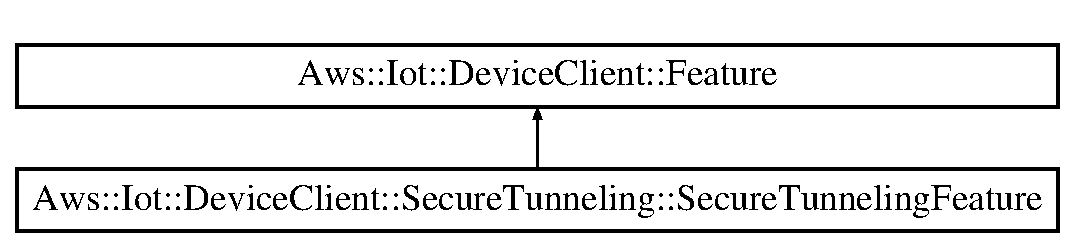
\includegraphics[height=2.000000cm]{class_aws_1_1_iot_1_1_device_client_1_1_secure_tunneling_1_1_secure_tunneling_feature}
\end{center}
\end{figure}
\doxysubsection*{Public Member Functions}
\begin{DoxyCompactItemize}
\item 
\mbox{\Hypertarget{class_aws_1_1_iot_1_1_device_client_1_1_secure_tunneling_1_1_secure_tunneling_feature_a91ae57f57ac24b8da585356f47981d94}\label{class_aws_1_1_iot_1_1_device_client_1_1_secure_tunneling_1_1_secure_tunneling_feature_a91ae57f57ac24b8da585356f47981d94}} 
\mbox{\hyperlink{class_aws_1_1_iot_1_1_device_client_1_1_secure_tunneling_1_1_secure_tunneling_feature_a91ae57f57ac24b8da585356f47981d94}{Secure\+Tunneling\+Feature}} ()
\begin{DoxyCompactList}\small\item\em Constructor. \end{DoxyCompactList}\item 
\mbox{\Hypertarget{class_aws_1_1_iot_1_1_device_client_1_1_secure_tunneling_1_1_secure_tunneling_feature_a90c1083b18d61d7dc8a7018e54494e09}\label{class_aws_1_1_iot_1_1_device_client_1_1_secure_tunneling_1_1_secure_tunneling_feature_a90c1083b18d61d7dc8a7018e54494e09}} 
\mbox{\hyperlink{class_aws_1_1_iot_1_1_device_client_1_1_secure_tunneling_1_1_secure_tunneling_feature_a90c1083b18d61d7dc8a7018e54494e09}{$\sim$\+Secure\+Tunneling\+Feature}} () override
\begin{DoxyCompactList}\small\item\em Destructor. \end{DoxyCompactList}\item 
int \mbox{\hyperlink{class_aws_1_1_iot_1_1_device_client_1_1_secure_tunneling_1_1_secure_tunneling_feature_ae8600a395ea715e35ccd12a8f79be34c}{init}} (std\+::shared\+\_\+ptr$<$ \mbox{\hyperlink{class_aws_1_1_iot_1_1_device_client_1_1_shared_crt_resource_manager}{Shared\+Crt\+Resource\+Manager}} $>$ manager, std\+::shared\+\_\+ptr$<$ \mbox{\hyperlink{class_aws_1_1_iot_1_1_device_client_1_1_client_base_notifier}{Client\+Base\+Notifier}} $>$ notifier, const \mbox{\hyperlink{struct_aws_1_1_iot_1_1_device_client_1_1_plain_config}{Plain\+Config}} \&config)
\begin{DoxyCompactList}\small\item\em Initializes the Secure Tunneling feature with all the required setup information, event handlers, and the shared Mqtt\+Connection. \end{DoxyCompactList}\item 
std\+::string \mbox{\hyperlink{class_aws_1_1_iot_1_1_device_client_1_1_secure_tunneling_1_1_secure_tunneling_feature_accc93db855be85847c3472754439594f}{get\+Name}} () override
\begin{DoxyCompactList}\small\item\em For a given feature, returns its name. \end{DoxyCompactList}\item 
int \mbox{\hyperlink{class_aws_1_1_iot_1_1_device_client_1_1_secure_tunneling_1_1_secure_tunneling_feature_a9e33fc786883e519e587f7d89f2a9086}{start}} () override
\begin{DoxyCompactList}\small\item\em Start the feature. \end{DoxyCompactList}\item 
int \mbox{\hyperlink{class_aws_1_1_iot_1_1_device_client_1_1_secure_tunneling_1_1_secure_tunneling_feature_a9cd3840b50bd1f62537df3354c7d2fbf}{stop}} () override
\begin{DoxyCompactList}\small\item\em Stop the feature. \end{DoxyCompactList}\end{DoxyCompactItemize}
\doxysubsection*{Static Public Member Functions}
\begin{DoxyCompactItemize}
\item 
static uint16\+\_\+t \mbox{\hyperlink{class_aws_1_1_iot_1_1_device_client_1_1_secure_tunneling_1_1_secure_tunneling_feature_af9e304cd7e3eb06cd2358b3e9fe838c0}{Get\+Port\+From\+Service}} (const std\+::string \&service)
\begin{DoxyCompactList}\small\item\em Returns the port number of the given service. \end{DoxyCompactList}\item 
static bool \mbox{\hyperlink{class_aws_1_1_iot_1_1_device_client_1_1_secure_tunneling_1_1_secure_tunneling_feature_a40e54cf67d52c08f73d8b5486e846bac}{Is\+Valid\+Port}} (int port)
\begin{DoxyCompactList}\small\item\em Check if the given port is within the valid range. \end{DoxyCompactList}\end{DoxyCompactItemize}
\doxysubsection*{Private Member Functions}
\begin{DoxyCompactItemize}
\item 
void \mbox{\hyperlink{class_aws_1_1_iot_1_1_device_client_1_1_secure_tunneling_1_1_secure_tunneling_feature_a72e0cfcb7782c86dc8e7595cac703009}{Load\+From\+Config}} (const \mbox{\hyperlink{struct_aws_1_1_iot_1_1_device_client_1_1_plain_config}{Plain\+Config}} \&config)
\begin{DoxyCompactList}\small\item\em Load configuration data from the config object. \end{DoxyCompactList}\item 
\mbox{\Hypertarget{class_aws_1_1_iot_1_1_device_client_1_1_secure_tunneling_1_1_secure_tunneling_feature_a5c65f96aad2c5018af0633f590d4af0c}\label{class_aws_1_1_iot_1_1_device_client_1_1_secure_tunneling_1_1_secure_tunneling_feature_a5c65f96aad2c5018af0633f590d4af0c}} 
void \mbox{\hyperlink{class_aws_1_1_iot_1_1_device_client_1_1_secure_tunneling_1_1_secure_tunneling_feature_a5c65f96aad2c5018af0633f590d4af0c}{Run\+Secure\+Tunneling}} ()
\begin{DoxyCompactList}\small\item\em Run the Secure Tunneling feature. \end{DoxyCompactList}\item 
void \mbox{\hyperlink{class_aws_1_1_iot_1_1_device_client_1_1_secure_tunneling_1_1_secure_tunneling_feature_ac865de9e5b5a8ae64911d9fcfc83750b}{On\+Subscribe\+To\+Tunnels\+Notify\+Response}} (Aws\+::\+Iotsecuretunneling\+::\+Secure\+Tunneling\+Notify\+Response $\ast$response, int io\+Err)
\begin{DoxyCompactList}\small\item\em Callback when a M\+Q\+TT new tunnel notification is received. \end{DoxyCompactList}\item 
void \mbox{\hyperlink{class_aws_1_1_iot_1_1_device_client_1_1_secure_tunneling_1_1_secure_tunneling_feature_ac883c84d52e745b2e58b039c60416d09}{On\+Subscribe\+Complete}} (int io\+Err)
\begin{DoxyCompactList}\small\item\em Callback when subscribe to M\+Q\+TT new tunnel notification is complete. \end{DoxyCompactList}\item 
std\+::string \mbox{\hyperlink{class_aws_1_1_iot_1_1_device_client_1_1_secure_tunneling_1_1_secure_tunneling_feature_a930dcd5d280ecc9ae591f6f9a8cf3c0a}{Get\+Endpoint}} (const std\+::string \&region)
\begin{DoxyCompactList}\small\item\em Get the secure tunneling data plain endpoint given an A\+WS region. \end{DoxyCompactList}\item 
void \mbox{\hyperlink{class_aws_1_1_iot_1_1_device_client_1_1_secure_tunneling_1_1_secure_tunneling_feature_afb34e3a40f628b963992e5187b8fc596}{On\+Connection\+Shutdown}} (\mbox{\hyperlink{class_aws_1_1_iot_1_1_device_client_1_1_secure_tunneling_1_1_secure_tunneling_context}{Secure\+Tunneling\+Context}} $\ast$context\+To\+Remove)
\begin{DoxyCompactList}\small\item\em Callback when a secure tunnel is shutdown. \end{DoxyCompactList}\end{DoxyCompactItemize}
\doxysubsection*{Private Attributes}
\begin{DoxyCompactItemize}
\item 
\mbox{\Hypertarget{class_aws_1_1_iot_1_1_device_client_1_1_secure_tunneling_1_1_secure_tunneling_feature_ab7c083e3e44ccc4c68230103b3052d84}\label{class_aws_1_1_iot_1_1_device_client_1_1_secure_tunneling_1_1_secure_tunneling_feature_ab7c083e3e44ccc4c68230103b3052d84}} 
std\+::shared\+\_\+ptr$<$ \mbox{\hyperlink{class_aws_1_1_iot_1_1_device_client_1_1_shared_crt_resource_manager}{Shared\+Crt\+Resource\+Manager}} $>$ \mbox{\hyperlink{class_aws_1_1_iot_1_1_device_client_1_1_secure_tunneling_1_1_secure_tunneling_feature_ab7c083e3e44ccc4c68230103b3052d84}{m\+Shared\+Crt\+Resource\+Manager}}
\begin{DoxyCompactList}\small\item\em The resource manager used to manage C\+RT resources. \end{DoxyCompactList}\item 
\mbox{\Hypertarget{class_aws_1_1_iot_1_1_device_client_1_1_secure_tunneling_1_1_secure_tunneling_feature_a2bad62761f33272e901f3c9046ba4e20}\label{class_aws_1_1_iot_1_1_device_client_1_1_secure_tunneling_1_1_secure_tunneling_feature_a2bad62761f33272e901f3c9046ba4e20}} 
std\+::unique\+\_\+ptr$<$ Aws\+::\+Iotdevicecommon\+::\+Device\+Api\+Handle $>$ \mbox{\hyperlink{class_aws_1_1_iot_1_1_device_client_1_1_secure_tunneling_1_1_secure_tunneling_feature_a2bad62761f33272e901f3c9046ba4e20}{m\+Device\+Api\+Handle}}
\begin{DoxyCompactList}\small\item\em A resource required to initialize the IoT S\+DK. \end{DoxyCompactList}\item 
\mbox{\Hypertarget{class_aws_1_1_iot_1_1_device_client_1_1_secure_tunneling_1_1_secure_tunneling_feature_a3bec48f8bae11a8b070409a1c6d5a5b4}\label{class_aws_1_1_iot_1_1_device_client_1_1_secure_tunneling_1_1_secure_tunneling_feature_a3bec48f8bae11a8b070409a1c6d5a5b4}} 
std\+::shared\+\_\+ptr$<$ \mbox{\hyperlink{class_aws_1_1_iot_1_1_device_client_1_1_client_base_notifier}{Client\+Base\+Notifier}} $>$ \mbox{\hyperlink{class_aws_1_1_iot_1_1_device_client_1_1_secure_tunneling_1_1_secure_tunneling_feature_a3bec48f8bae11a8b070409a1c6d5a5b4}{m\+Client\+Base\+Notifier}}
\begin{DoxyCompactList}\small\item\em An object used to notify the Client base if there is an event that requires its attention. \end{DoxyCompactList}\item 
\mbox{\Hypertarget{class_aws_1_1_iot_1_1_device_client_1_1_secure_tunneling_1_1_secure_tunneling_feature_af374641c2f33bc8985af08b26d0fb6d1}\label{class_aws_1_1_iot_1_1_device_client_1_1_secure_tunneling_1_1_secure_tunneling_feature_af374641c2f33bc8985af08b26d0fb6d1}} 
std\+::string \mbox{\hyperlink{class_aws_1_1_iot_1_1_device_client_1_1_secure_tunneling_1_1_secure_tunneling_feature_af374641c2f33bc8985af08b26d0fb6d1}{m\+Thing\+Name}}
\begin{DoxyCompactList}\small\item\em The Thing\+Name to use. \end{DoxyCompactList}\item 
\mbox{\Hypertarget{class_aws_1_1_iot_1_1_device_client_1_1_secure_tunneling_1_1_secure_tunneling_feature_a1b59b829f560cebd8b58189bc0479f95}\label{class_aws_1_1_iot_1_1_device_client_1_1_secure_tunneling_1_1_secure_tunneling_feature_a1b59b829f560cebd8b58189bc0479f95}} 
std\+::string \mbox{\hyperlink{class_aws_1_1_iot_1_1_device_client_1_1_secure_tunneling_1_1_secure_tunneling_feature_a1b59b829f560cebd8b58189bc0479f95}{m\+Root\+Ca}}
\begin{DoxyCompactList}\small\item\em Path to the Amazon root CA. \end{DoxyCompactList}\item 
\mbox{\Hypertarget{class_aws_1_1_iot_1_1_device_client_1_1_secure_tunneling_1_1_secure_tunneling_feature_a85ec525712376af69f99ae024a28fb55}\label{class_aws_1_1_iot_1_1_device_client_1_1_secure_tunneling_1_1_secure_tunneling_feature_a85ec525712376af69f99ae024a28fb55}} 
bool \mbox{\hyperlink{class_aws_1_1_iot_1_1_device_client_1_1_secure_tunneling_1_1_secure_tunneling_feature_a85ec525712376af69f99ae024a28fb55}{m\+Subscribe\+Notification}} \{true\}
\begin{DoxyCompactList}\small\item\em Should the Secure Tunneling feature subscribe to M\+Q\+TT new tunnel notification? \end{DoxyCompactList}\item 
\mbox{\Hypertarget{class_aws_1_1_iot_1_1_device_client_1_1_secure_tunneling_1_1_secure_tunneling_feature_a214e9168c8d239bd8d33c4bfe33fce95}\label{class_aws_1_1_iot_1_1_device_client_1_1_secure_tunneling_1_1_secure_tunneling_feature_a214e9168c8d239bd8d33c4bfe33fce95}} 
Aws\+::\+Crt\+::\+Optional$<$ std\+::string $>$ \mbox{\hyperlink{class_aws_1_1_iot_1_1_device_client_1_1_secure_tunneling_1_1_secure_tunneling_feature_a214e9168c8d239bd8d33c4bfe33fce95}{m\+Endpoint}}
\begin{DoxyCompactList}\small\item\em Endpoint override. Normally the endpoint is determined by {\ttfamily region} only. This is only used to override the normal endpoint such as when testing against the gamma stage. \end{DoxyCompactList}\item 
\mbox{\Hypertarget{class_aws_1_1_iot_1_1_device_client_1_1_secure_tunneling_1_1_secure_tunneling_feature_a4e2431941bc9e6e9f30415122bfdb610}\label{class_aws_1_1_iot_1_1_device_client_1_1_secure_tunneling_1_1_secure_tunneling_feature_a4e2431941bc9e6e9f30415122bfdb610}} 
std\+::vector$<$ std\+::unique\+\_\+ptr$<$ \mbox{\hyperlink{class_aws_1_1_iot_1_1_device_client_1_1_secure_tunneling_1_1_secure_tunneling_context}{Secure\+Tunneling\+Context}} $>$ $>$ \mbox{\hyperlink{class_aws_1_1_iot_1_1_device_client_1_1_secure_tunneling_1_1_secure_tunneling_feature_a4e2431941bc9e6e9f30415122bfdb610}{m\+Contexts}}
\begin{DoxyCompactList}\small\item\em A vector of \mbox{\hyperlink{class_aws_1_1_iot_1_1_device_client_1_1_secure_tunneling_1_1_secure_tunneling_context}{Secure\+Tunneling\+Context}}. Each context represents an active secure tunneling session. \end{DoxyCompactList}\end{DoxyCompactItemize}
\doxysubsection*{Static Private Attributes}
\begin{DoxyCompactItemize}
\item 
\mbox{\Hypertarget{class_aws_1_1_iot_1_1_device_client_1_1_secure_tunneling_1_1_secure_tunneling_feature_a7d700b7591d51240c6aca5b579ab810e}\label{class_aws_1_1_iot_1_1_device_client_1_1_secure_tunneling_1_1_secure_tunneling_feature_a7d700b7591d51240c6aca5b579ab810e}} 
static constexpr char \mbox{\hyperlink{class_aws_1_1_iot_1_1_device_client_1_1_secure_tunneling_1_1_secure_tunneling_feature_a7d700b7591d51240c6aca5b579ab810e}{T\+AG}} \mbox{[}$\,$\mbox{]} = \char`\"{}Secure\+Tunneling.\+cpp\char`\"{}
\begin{DoxyCompactList}\small\item\em Used by the logger to specify that log messages are coming from the Secure Tunneling feature. \end{DoxyCompactList}\item 
\mbox{\Hypertarget{class_aws_1_1_iot_1_1_device_client_1_1_secure_tunneling_1_1_secure_tunneling_feature_a8834fc640c69a3ed47fc57e3b59a8923}\label{class_aws_1_1_iot_1_1_device_client_1_1_secure_tunneling_1_1_secure_tunneling_feature_a8834fc640c69a3ed47fc57e3b59a8923}} 
static constexpr char \mbox{\hyperlink{class_aws_1_1_iot_1_1_device_client_1_1_secure_tunneling_1_1_secure_tunneling_feature_a8834fc640c69a3ed47fc57e3b59a8923}{D\+E\+F\+A\+U\+L\+T\+\_\+\+P\+R\+O\+X\+Y\+\_\+\+E\+N\+D\+P\+O\+I\+N\+T\+\_\+\+H\+O\+S\+T\+\_\+\+F\+O\+R\+M\+AT}} \mbox{[}$\,$\mbox{]} = \char`\"{}data.\+tunneling.\+iot.\%s.\+amazonaws.\+com\char`\"{}
\begin{DoxyCompactList}\small\item\em Format string for forming the secure tunneling data plain endpoint. \end{DoxyCompactList}\item 
\mbox{\Hypertarget{class_aws_1_1_iot_1_1_device_client_1_1_secure_tunneling_1_1_secure_tunneling_feature_aeaafb01665e10b726f93f5247767193e}\label{class_aws_1_1_iot_1_1_device_client_1_1_secure_tunneling_1_1_secure_tunneling_feature_aeaafb01665e10b726f93f5247767193e}} 
static std\+::map$<$ std\+::string, uint16\+\_\+t $>$ \mbox{\hyperlink{class_aws_1_1_iot_1_1_device_client_1_1_secure_tunneling_1_1_secure_tunneling_feature_aeaafb01665e10b726f93f5247767193e}{m\+Service\+To\+Port\+Map}}
\begin{DoxyCompactList}\small\item\em A map for converting supported services to their port numbers. \end{DoxyCompactList}\end{DoxyCompactItemize}


\doxysubsection{Detailed Description}
Provides IoT Secure Tunneling related functionality within the Device Client. 

\doxysubsection{Member Function Documentation}
\mbox{\Hypertarget{class_aws_1_1_iot_1_1_device_client_1_1_secure_tunneling_1_1_secure_tunneling_feature_a930dcd5d280ecc9ae591f6f9a8cf3c0a}\label{class_aws_1_1_iot_1_1_device_client_1_1_secure_tunneling_1_1_secure_tunneling_feature_a930dcd5d280ecc9ae591f6f9a8cf3c0a}} 
\index{Aws::Iot::DeviceClient::SecureTunneling::SecureTunnelingFeature@{Aws::Iot::DeviceClient::SecureTunneling::SecureTunnelingFeature}!GetEndpoint@{GetEndpoint}}
\index{GetEndpoint@{GetEndpoint}!Aws::Iot::DeviceClient::SecureTunneling::SecureTunnelingFeature@{Aws::Iot::DeviceClient::SecureTunneling::SecureTunnelingFeature}}
\doxysubsubsection{\texorpdfstring{GetEndpoint()}{GetEndpoint()}}
{\footnotesize\ttfamily string Aws\+::\+Iot\+::\+Device\+Client\+::\+Secure\+Tunneling\+::\+Secure\+Tunneling\+Feature\+::\+Get\+Endpoint (\begin{DoxyParamCaption}\item[{const std\+::string \&}]{region }\end{DoxyParamCaption})\hspace{0.3cm}{\ttfamily [private]}}



Get the secure tunneling data plain endpoint given an A\+WS region. 


\begin{DoxyParams}{Parameters}
{\em region} & A\+WS region \\
\hline
\end{DoxyParams}
\begin{DoxyReturn}{Returns}
Secure Tunneling data plain endpoint 
\end{DoxyReturn}
\mbox{\Hypertarget{class_aws_1_1_iot_1_1_device_client_1_1_secure_tunneling_1_1_secure_tunneling_feature_accc93db855be85847c3472754439594f}\label{class_aws_1_1_iot_1_1_device_client_1_1_secure_tunneling_1_1_secure_tunneling_feature_accc93db855be85847c3472754439594f}} 
\index{Aws::Iot::DeviceClient::SecureTunneling::SecureTunnelingFeature@{Aws::Iot::DeviceClient::SecureTunneling::SecureTunnelingFeature}!getName@{getName}}
\index{getName@{getName}!Aws::Iot::DeviceClient::SecureTunneling::SecureTunnelingFeature@{Aws::Iot::DeviceClient::SecureTunneling::SecureTunnelingFeature}}
\doxysubsubsection{\texorpdfstring{getName()}{getName()}}
{\footnotesize\ttfamily string Aws\+::\+Iot\+::\+Device\+Client\+::\+Secure\+Tunneling\+::\+Secure\+Tunneling\+Feature\+::get\+Name (\begin{DoxyParamCaption}{ }\end{DoxyParamCaption})\hspace{0.3cm}{\ttfamily [override]}, {\ttfamily [virtual]}}



For a given feature, returns its name. 

\begin{DoxyReturn}{Returns}
a string value representing the feature\textquotesingle{}s name 
\end{DoxyReturn}


Implements \mbox{\hyperlink{class_aws_1_1_iot_1_1_device_client_1_1_feature_a7f56b81457898d67ddc1942e57e3c0d5}{Aws\+::\+Iot\+::\+Device\+Client\+::\+Feature}}.

\mbox{\Hypertarget{class_aws_1_1_iot_1_1_device_client_1_1_secure_tunneling_1_1_secure_tunneling_feature_af9e304cd7e3eb06cd2358b3e9fe838c0}\label{class_aws_1_1_iot_1_1_device_client_1_1_secure_tunneling_1_1_secure_tunneling_feature_af9e304cd7e3eb06cd2358b3e9fe838c0}} 
\index{Aws::Iot::DeviceClient::SecureTunneling::SecureTunnelingFeature@{Aws::Iot::DeviceClient::SecureTunneling::SecureTunnelingFeature}!GetPortFromService@{GetPortFromService}}
\index{GetPortFromService@{GetPortFromService}!Aws::Iot::DeviceClient::SecureTunneling::SecureTunnelingFeature@{Aws::Iot::DeviceClient::SecureTunneling::SecureTunnelingFeature}}
\doxysubsubsection{\texorpdfstring{GetPortFromService()}{GetPortFromService()}}
{\footnotesize\ttfamily uint16\+\_\+t Aws\+::\+Iot\+::\+Device\+Client\+::\+Secure\+Tunneling\+::\+Secure\+Tunneling\+Feature\+::\+Get\+Port\+From\+Service (\begin{DoxyParamCaption}\item[{const std\+::string \&}]{service }\end{DoxyParamCaption})\hspace{0.3cm}{\ttfamily [static]}}



Returns the port number of the given service. 


\begin{DoxyParams}{Parameters}
{\em service} & the name of the service \\
\hline
\end{DoxyParams}
\begin{DoxyReturn}{Returns}
the port number 
\end{DoxyReturn}
\mbox{\Hypertarget{class_aws_1_1_iot_1_1_device_client_1_1_secure_tunneling_1_1_secure_tunneling_feature_ae8600a395ea715e35ccd12a8f79be34c}\label{class_aws_1_1_iot_1_1_device_client_1_1_secure_tunneling_1_1_secure_tunneling_feature_ae8600a395ea715e35ccd12a8f79be34c}} 
\index{Aws::Iot::DeviceClient::SecureTunneling::SecureTunnelingFeature@{Aws::Iot::DeviceClient::SecureTunneling::SecureTunnelingFeature}!init@{init}}
\index{init@{init}!Aws::Iot::DeviceClient::SecureTunneling::SecureTunnelingFeature@{Aws::Iot::DeviceClient::SecureTunneling::SecureTunnelingFeature}}
\doxysubsubsection{\texorpdfstring{init()}{init()}}
{\footnotesize\ttfamily int Aws\+::\+Iot\+::\+Device\+Client\+::\+Secure\+Tunneling\+::\+Secure\+Tunneling\+Feature\+::init (\begin{DoxyParamCaption}\item[{std\+::shared\+\_\+ptr$<$ \mbox{\hyperlink{class_aws_1_1_iot_1_1_device_client_1_1_shared_crt_resource_manager}{Shared\+Crt\+Resource\+Manager}} $>$}]{manager,  }\item[{std\+::shared\+\_\+ptr$<$ \mbox{\hyperlink{class_aws_1_1_iot_1_1_device_client_1_1_client_base_notifier}{Client\+Base\+Notifier}} $>$}]{notifier,  }\item[{const \mbox{\hyperlink{struct_aws_1_1_iot_1_1_device_client_1_1_plain_config}{Plain\+Config}} \&}]{config }\end{DoxyParamCaption})}



Initializes the Secure Tunneling feature with all the required setup information, event handlers, and the shared Mqtt\+Connection. 


\begin{DoxyParams}{Parameters}
{\em manager} & the shared resource manager \\
\hline
{\em notifier} & an \mbox{\hyperlink{class_aws_1_1_iot_1_1_device_client_1_1_client_base_notifier}{Client\+Base\+Notifier}} used for notifying the client base of events or errors \\
\hline
{\em config} & configuration information passed in by the user via either the command line or configuration file \\
\hline
\end{DoxyParams}
\begin{DoxyReturn}{Returns}
a non-\/zero return code indicates a problem. The logs can be checked for more info 
\end{DoxyReturn}
\mbox{\Hypertarget{class_aws_1_1_iot_1_1_device_client_1_1_secure_tunneling_1_1_secure_tunneling_feature_a40e54cf67d52c08f73d8b5486e846bac}\label{class_aws_1_1_iot_1_1_device_client_1_1_secure_tunneling_1_1_secure_tunneling_feature_a40e54cf67d52c08f73d8b5486e846bac}} 
\index{Aws::Iot::DeviceClient::SecureTunneling::SecureTunnelingFeature@{Aws::Iot::DeviceClient::SecureTunneling::SecureTunnelingFeature}!IsValidPort@{IsValidPort}}
\index{IsValidPort@{IsValidPort}!Aws::Iot::DeviceClient::SecureTunneling::SecureTunnelingFeature@{Aws::Iot::DeviceClient::SecureTunneling::SecureTunnelingFeature}}
\doxysubsubsection{\texorpdfstring{IsValidPort()}{IsValidPort()}}
{\footnotesize\ttfamily bool Aws\+::\+Iot\+::\+Device\+Client\+::\+Secure\+Tunneling\+::\+Secure\+Tunneling\+Feature\+::\+Is\+Valid\+Port (\begin{DoxyParamCaption}\item[{int}]{port }\end{DoxyParamCaption})\hspace{0.3cm}{\ttfamily [static]}}



Check if the given port is within the valid range. 


\begin{DoxyParams}{Parameters}
{\em port} & the port to check \\
\hline
\end{DoxyParams}
\begin{DoxyReturn}{Returns}
True if the port is within the valid range. False otherwise. 
\end{DoxyReturn}
\mbox{\Hypertarget{class_aws_1_1_iot_1_1_device_client_1_1_secure_tunneling_1_1_secure_tunneling_feature_a72e0cfcb7782c86dc8e7595cac703009}\label{class_aws_1_1_iot_1_1_device_client_1_1_secure_tunneling_1_1_secure_tunneling_feature_a72e0cfcb7782c86dc8e7595cac703009}} 
\index{Aws::Iot::DeviceClient::SecureTunneling::SecureTunnelingFeature@{Aws::Iot::DeviceClient::SecureTunneling::SecureTunnelingFeature}!LoadFromConfig@{LoadFromConfig}}
\index{LoadFromConfig@{LoadFromConfig}!Aws::Iot::DeviceClient::SecureTunneling::SecureTunnelingFeature@{Aws::Iot::DeviceClient::SecureTunneling::SecureTunnelingFeature}}
\doxysubsubsection{\texorpdfstring{LoadFromConfig()}{LoadFromConfig()}}
{\footnotesize\ttfamily void Aws\+::\+Iot\+::\+Device\+Client\+::\+Secure\+Tunneling\+::\+Secure\+Tunneling\+Feature\+::\+Load\+From\+Config (\begin{DoxyParamCaption}\item[{const \mbox{\hyperlink{struct_aws_1_1_iot_1_1_device_client_1_1_plain_config}{Plain\+Config}} \&}]{config }\end{DoxyParamCaption})\hspace{0.3cm}{\ttfamily [private]}}



Load configuration data from the config object. 


\begin{DoxyParams}{Parameters}
{\em config} & the configuration object to load from \\
\hline
\end{DoxyParams}
\mbox{\Hypertarget{class_aws_1_1_iot_1_1_device_client_1_1_secure_tunneling_1_1_secure_tunneling_feature_afb34e3a40f628b963992e5187b8fc596}\label{class_aws_1_1_iot_1_1_device_client_1_1_secure_tunneling_1_1_secure_tunneling_feature_afb34e3a40f628b963992e5187b8fc596}} 
\index{Aws::Iot::DeviceClient::SecureTunneling::SecureTunnelingFeature@{Aws::Iot::DeviceClient::SecureTunneling::SecureTunnelingFeature}!OnConnectionShutdown@{OnConnectionShutdown}}
\index{OnConnectionShutdown@{OnConnectionShutdown}!Aws::Iot::DeviceClient::SecureTunneling::SecureTunnelingFeature@{Aws::Iot::DeviceClient::SecureTunneling::SecureTunnelingFeature}}
\doxysubsubsection{\texorpdfstring{OnConnectionShutdown()}{OnConnectionShutdown()}}
{\footnotesize\ttfamily void Aws\+::\+Iot\+::\+Device\+Client\+::\+Secure\+Tunneling\+::\+Secure\+Tunneling\+Feature\+::\+On\+Connection\+Shutdown (\begin{DoxyParamCaption}\item[{\mbox{\hyperlink{class_aws_1_1_iot_1_1_device_client_1_1_secure_tunneling_1_1_secure_tunneling_context}{Secure\+Tunneling\+Context}} $\ast$}]{context\+To\+Remove }\end{DoxyParamCaption})\hspace{0.3cm}{\ttfamily [private]}}



Callback when a secure tunnel is shutdown. 


\begin{DoxyParams}{Parameters}
{\em context\+To\+Remove} & a \mbox{\hyperlink{class_aws_1_1_iot_1_1_device_client_1_1_secure_tunneling_1_1_secure_tunneling_context}{Secure\+Tunneling\+Context}} that represents the secure tunnel that was shutdown \\
\hline
\end{DoxyParams}
\mbox{\Hypertarget{class_aws_1_1_iot_1_1_device_client_1_1_secure_tunneling_1_1_secure_tunneling_feature_ac883c84d52e745b2e58b039c60416d09}\label{class_aws_1_1_iot_1_1_device_client_1_1_secure_tunneling_1_1_secure_tunneling_feature_ac883c84d52e745b2e58b039c60416d09}} 
\index{Aws::Iot::DeviceClient::SecureTunneling::SecureTunnelingFeature@{Aws::Iot::DeviceClient::SecureTunneling::SecureTunnelingFeature}!OnSubscribeComplete@{OnSubscribeComplete}}
\index{OnSubscribeComplete@{OnSubscribeComplete}!Aws::Iot::DeviceClient::SecureTunneling::SecureTunnelingFeature@{Aws::Iot::DeviceClient::SecureTunneling::SecureTunnelingFeature}}
\doxysubsubsection{\texorpdfstring{OnSubscribeComplete()}{OnSubscribeComplete()}}
{\footnotesize\ttfamily void Aws\+::\+Iot\+::\+Device\+Client\+::\+Secure\+Tunneling\+::\+Secure\+Tunneling\+Feature\+::\+On\+Subscribe\+Complete (\begin{DoxyParamCaption}\item[{int}]{io\+Err }\end{DoxyParamCaption})\hspace{0.3cm}{\ttfamily [private]}}



Callback when subscribe to M\+Q\+TT new tunnel notification is complete. 


\begin{DoxyParams}{Parameters}
{\em io\+Err} & error code \\
\hline
\end{DoxyParams}
\mbox{\Hypertarget{class_aws_1_1_iot_1_1_device_client_1_1_secure_tunneling_1_1_secure_tunneling_feature_ac865de9e5b5a8ae64911d9fcfc83750b}\label{class_aws_1_1_iot_1_1_device_client_1_1_secure_tunneling_1_1_secure_tunneling_feature_ac865de9e5b5a8ae64911d9fcfc83750b}} 
\index{Aws::Iot::DeviceClient::SecureTunneling::SecureTunnelingFeature@{Aws::Iot::DeviceClient::SecureTunneling::SecureTunnelingFeature}!OnSubscribeToTunnelsNotifyResponse@{OnSubscribeToTunnelsNotifyResponse}}
\index{OnSubscribeToTunnelsNotifyResponse@{OnSubscribeToTunnelsNotifyResponse}!Aws::Iot::DeviceClient::SecureTunneling::SecureTunnelingFeature@{Aws::Iot::DeviceClient::SecureTunneling::SecureTunnelingFeature}}
\doxysubsubsection{\texorpdfstring{OnSubscribeToTunnelsNotifyResponse()}{OnSubscribeToTunnelsNotifyResponse()}}
{\footnotesize\ttfamily void Aws\+::\+Iot\+::\+Device\+Client\+::\+Secure\+Tunneling\+::\+Secure\+Tunneling\+Feature\+::\+On\+Subscribe\+To\+Tunnels\+Notify\+Response (\begin{DoxyParamCaption}\item[{Aws\+::\+Iotsecuretunneling\+::\+Secure\+Tunneling\+Notify\+Response $\ast$}]{response,  }\item[{int}]{io\+Err }\end{DoxyParamCaption})\hspace{0.3cm}{\ttfamily [private]}}



Callback when a M\+Q\+TT new tunnel notification is received. 


\begin{DoxyParams}{Parameters}
{\em response} & M\+Q\+TT new tunnel notification \\
\hline
{\em io\+Err} & error code \\
\hline
\end{DoxyParams}
\mbox{\Hypertarget{class_aws_1_1_iot_1_1_device_client_1_1_secure_tunneling_1_1_secure_tunneling_feature_a9e33fc786883e519e587f7d89f2a9086}\label{class_aws_1_1_iot_1_1_device_client_1_1_secure_tunneling_1_1_secure_tunneling_feature_a9e33fc786883e519e587f7d89f2a9086}} 
\index{Aws::Iot::DeviceClient::SecureTunneling::SecureTunnelingFeature@{Aws::Iot::DeviceClient::SecureTunneling::SecureTunnelingFeature}!start@{start}}
\index{start@{start}!Aws::Iot::DeviceClient::SecureTunneling::SecureTunnelingFeature@{Aws::Iot::DeviceClient::SecureTunneling::SecureTunnelingFeature}}
\doxysubsubsection{\texorpdfstring{start()}{start()}}
{\footnotesize\ttfamily int Aws\+::\+Iot\+::\+Device\+Client\+::\+Secure\+Tunneling\+::\+Secure\+Tunneling\+Feature\+::start (\begin{DoxyParamCaption}{ }\end{DoxyParamCaption})\hspace{0.3cm}{\ttfamily [override]}, {\ttfamily [virtual]}}



Start the feature. 

\begin{DoxyReturn}{Returns}
an integer representing the S\+U\+C\+C\+E\+SS or F\+A\+I\+L\+U\+RE of the \mbox{\hyperlink{class_aws_1_1_iot_1_1_device_client_1_1_secure_tunneling_1_1_secure_tunneling_feature_a9e33fc786883e519e587f7d89f2a9086}{start()}} operation on the feature 
\end{DoxyReturn}


Implements \mbox{\hyperlink{class_aws_1_1_iot_1_1_device_client_1_1_feature_ac9a936ebd88f7e35914a6aac99badf7d}{Aws\+::\+Iot\+::\+Device\+Client\+::\+Feature}}.

\mbox{\Hypertarget{class_aws_1_1_iot_1_1_device_client_1_1_secure_tunneling_1_1_secure_tunneling_feature_a9cd3840b50bd1f62537df3354c7d2fbf}\label{class_aws_1_1_iot_1_1_device_client_1_1_secure_tunneling_1_1_secure_tunneling_feature_a9cd3840b50bd1f62537df3354c7d2fbf}} 
\index{Aws::Iot::DeviceClient::SecureTunneling::SecureTunnelingFeature@{Aws::Iot::DeviceClient::SecureTunneling::SecureTunnelingFeature}!stop@{stop}}
\index{stop@{stop}!Aws::Iot::DeviceClient::SecureTunneling::SecureTunnelingFeature@{Aws::Iot::DeviceClient::SecureTunneling::SecureTunnelingFeature}}
\doxysubsubsection{\texorpdfstring{stop()}{stop()}}
{\footnotesize\ttfamily int Aws\+::\+Iot\+::\+Device\+Client\+::\+Secure\+Tunneling\+::\+Secure\+Tunneling\+Feature\+::stop (\begin{DoxyParamCaption}{ }\end{DoxyParamCaption})\hspace{0.3cm}{\ttfamily [override]}, {\ttfamily [virtual]}}



Stop the feature. 

\begin{DoxyReturn}{Returns}
an integer representing the S\+U\+C\+C\+E\+SS or F\+A\+I\+L\+U\+RE of the \mbox{\hyperlink{class_aws_1_1_iot_1_1_device_client_1_1_secure_tunneling_1_1_secure_tunneling_feature_a9cd3840b50bd1f62537df3354c7d2fbf}{stop()}} operation on the feature 
\end{DoxyReturn}


Implements \mbox{\hyperlink{class_aws_1_1_iot_1_1_device_client_1_1_feature_a5b672f7b1403512cad9104ba923fc73d}{Aws\+::\+Iot\+::\+Device\+Client\+::\+Feature}}.



The documentation for this class was generated from the following files\+:\begin{DoxyCompactItemize}
\item 
/home/runner/work/aws-\/iot-\/device-\/client/aws-\/iot-\/device-\/client/source/tunneling/Secure\+Tunneling\+Feature.\+h\item 
/home/runner/work/aws-\/iot-\/device-\/client/aws-\/iot-\/device-\/client/source/tunneling/Secure\+Tunneling\+Feature.\+cpp\end{DoxyCompactItemize}

\hypertarget{class_aws_1_1_iot_1_1_device_client_1_1_shared_crt_resource_manager}{}\section{Aws\+:\+:Iot\+:\+:Device\+Client\+:\+:Shared\+Crt\+Resource\+Manager Class Reference}
\label{class_aws_1_1_iot_1_1_device_client_1_1_shared_crt_resource_manager}\index{Aws\+::\+Iot\+::\+Device\+Client\+::\+Shared\+Crt\+Resource\+Manager@{Aws\+::\+Iot\+::\+Device\+Client\+::\+Shared\+Crt\+Resource\+Manager}}


Utility class for managing the C\+RT S\+DK Resources.  




{\ttfamily \#include $<$Shared\+Crt\+Resource\+Manager.\+h$>$}

\subsection*{Public Member Functions}
\begin{DoxyCompactItemize}
\item 
\mbox{\Hypertarget{class_aws_1_1_iot_1_1_device_client_1_1_shared_crt_resource_manager_a8b8fc30a3b2e7b6ea9ebe1ad226959c6}\label{class_aws_1_1_iot_1_1_device_client_1_1_shared_crt_resource_manager_a8b8fc30a3b2e7b6ea9ebe1ad226959c6}} 
bool {\bfseries initialize} (const \hyperlink{struct_aws_1_1_iot_1_1_device_client_1_1_plain_config}{Plain\+Config} \&config)
\item 
\mbox{\Hypertarget{class_aws_1_1_iot_1_1_device_client_1_1_shared_crt_resource_manager_a38842906410bb0c7a1681eb6c97ccbca}\label{class_aws_1_1_iot_1_1_device_client_1_1_shared_crt_resource_manager_a38842906410bb0c7a1681eb6c97ccbca}} 
int {\bfseries establish\+Connection} (const \hyperlink{struct_aws_1_1_iot_1_1_device_client_1_1_plain_config}{Plain\+Config} \&config)
\item 
\mbox{\Hypertarget{class_aws_1_1_iot_1_1_device_client_1_1_shared_crt_resource_manager_a81cf347ae807249bd355c561dca95657}\label{class_aws_1_1_iot_1_1_device_client_1_1_shared_crt_resource_manager_a81cf347ae807249bd355c561dca95657}} 
std\+::shared\+\_\+ptr$<$ Crt\+::\+Mqtt\+::\+Mqtt\+Connection $>$ {\bfseries get\+Connection} ()
\item 
\mbox{\Hypertarget{class_aws_1_1_iot_1_1_device_client_1_1_shared_crt_resource_manager_a008f3a7fe2d537b4786bf56aa7fe6e0c}\label{class_aws_1_1_iot_1_1_device_client_1_1_shared_crt_resource_manager_a008f3a7fe2d537b4786bf56aa7fe6e0c}} 
Aws\+::\+Crt\+::\+Io\+::\+Event\+Loop\+Group $\ast$ {\bfseries get\+Event\+Loop\+Group} ()
\item 
\mbox{\Hypertarget{class_aws_1_1_iot_1_1_device_client_1_1_shared_crt_resource_manager_ab869efd973c78d6d30e9df7ba97e8a2e}\label{class_aws_1_1_iot_1_1_device_client_1_1_shared_crt_resource_manager_ab869efd973c78d6d30e9df7ba97e8a2e}} 
struct aws\+\_\+allocator $\ast$ {\bfseries get\+Allocator} ()
\item 
\mbox{\Hypertarget{class_aws_1_1_iot_1_1_device_client_1_1_shared_crt_resource_manager_ad758bebb8b5675cf08da79c60d4511b1}\label{class_aws_1_1_iot_1_1_device_client_1_1_shared_crt_resource_manager_ad758bebb8b5675cf08da79c60d4511b1}} 
Aws\+::\+Crt\+::\+Io\+::\+Client\+Bootstrap $\ast$ {\bfseries get\+Client\+Bootstrap} ()
\item 
\mbox{\Hypertarget{class_aws_1_1_iot_1_1_device_client_1_1_shared_crt_resource_manager_a2a1b26bc57897e2d81ddfa12bd080f0e}\label{class_aws_1_1_iot_1_1_device_client_1_1_shared_crt_resource_manager_a2a1b26bc57897e2d81ddfa12bd080f0e}} 
void {\bfseries disconnect} ()
\end{DoxyCompactItemize}
\subsection*{Static Public Attributes}
\begin{DoxyCompactItemize}
\item 
\mbox{\Hypertarget{class_aws_1_1_iot_1_1_device_client_1_1_shared_crt_resource_manager_ae853200444418700fe8c6c2384d1a981}\label{class_aws_1_1_iot_1_1_device_client_1_1_shared_crt_resource_manager_ae853200444418700fe8c6c2384d1a981}} 
static const int {\bfseries S\+U\+C\+C\+E\+SS} = 0
\item 
\mbox{\Hypertarget{class_aws_1_1_iot_1_1_device_client_1_1_shared_crt_resource_manager_a4ea6b778c387b63abeaee2d0099f6044}\label{class_aws_1_1_iot_1_1_device_client_1_1_shared_crt_resource_manager_a4ea6b778c387b63abeaee2d0099f6044}} 
static const int {\bfseries R\+E\+T\+RY} = 1
\item 
\mbox{\Hypertarget{class_aws_1_1_iot_1_1_device_client_1_1_shared_crt_resource_manager_a60e67742ab42176a7a1b3c9a4100779e}\label{class_aws_1_1_iot_1_1_device_client_1_1_shared_crt_resource_manager_a60e67742ab42176a7a1b3c9a4100779e}} 
static const int {\bfseries A\+B\+O\+RT} = 2
\end{DoxyCompactItemize}
\subsection*{Private Member Functions}
\begin{DoxyCompactItemize}
\item 
\mbox{\Hypertarget{class_aws_1_1_iot_1_1_device_client_1_1_shared_crt_resource_manager_a754e8d34e2ace5c551753c581653c254}\label{class_aws_1_1_iot_1_1_device_client_1_1_shared_crt_resource_manager_a754e8d34e2ace5c551753c581653c254}} 
bool {\bfseries locate\+Credentials} (const \hyperlink{struct_aws_1_1_iot_1_1_device_client_1_1_plain_config}{Plain\+Config} \&config)
\item 
\mbox{\Hypertarget{class_aws_1_1_iot_1_1_device_client_1_1_shared_crt_resource_manager_a4547bba8601c2dfce969476224e19061}\label{class_aws_1_1_iot_1_1_device_client_1_1_shared_crt_resource_manager_a4547bba8601c2dfce969476224e19061}} 
int {\bfseries build\+Client} ()
\item 
\mbox{\Hypertarget{class_aws_1_1_iot_1_1_device_client_1_1_shared_crt_resource_manager_a505c7645153752b656ec02614671e5f0}\label{class_aws_1_1_iot_1_1_device_client_1_1_shared_crt_resource_manager_a505c7645153752b656ec02614671e5f0}} 
void {\bfseries initialize\+Allocator} ()
\end{DoxyCompactItemize}
\subsection*{Private Attributes}
\begin{DoxyCompactItemize}
\item 
\mbox{\Hypertarget{class_aws_1_1_iot_1_1_device_client_1_1_shared_crt_resource_manager_a511ea1b492b39a073e486894ed3f0506}\label{class_aws_1_1_iot_1_1_device_client_1_1_shared_crt_resource_manager_a511ea1b492b39a073e486894ed3f0506}} 
const char $\ast$ {\bfseries T\+AG} = \char`\"{}Shared\+Crt\+Resource\+Manager.\+cpp\char`\"{}
\item 
\mbox{\Hypertarget{class_aws_1_1_iot_1_1_device_client_1_1_shared_crt_resource_manager_a1a2e7fffece11a2c67f9080bc0ac5bc8}\label{class_aws_1_1_iot_1_1_device_client_1_1_shared_crt_resource_manager_a1a2e7fffece11a2c67f9080bc0ac5bc8}} 
bool {\bfseries initialized} = false
\item 
\mbox{\Hypertarget{class_aws_1_1_iot_1_1_device_client_1_1_shared_crt_resource_manager_a57a29a339f8b7e9232c44a52bdd1e360}\label{class_aws_1_1_iot_1_1_device_client_1_1_shared_crt_resource_manager_a57a29a339f8b7e9232c44a52bdd1e360}} 
std\+::promise$<$ void $>$ {\bfseries connection\+Closed\+Promise}
\item 
\mbox{\Hypertarget{class_aws_1_1_iot_1_1_device_client_1_1_shared_crt_resource_manager_a77f6a022b928d747cf95e43a75f851ff}\label{class_aws_1_1_iot_1_1_device_client_1_1_shared_crt_resource_manager_a77f6a022b928d747cf95e43a75f851ff}} 
std\+::unique\+\_\+ptr$<$ Aws\+::\+Crt\+::\+Api\+Handle $>$ {\bfseries api\+Handle}
\item 
\mbox{\Hypertarget{class_aws_1_1_iot_1_1_device_client_1_1_shared_crt_resource_manager_af10d2d513b04cb58abc62641fbf3ff05}\label{class_aws_1_1_iot_1_1_device_client_1_1_shared_crt_resource_manager_af10d2d513b04cb58abc62641fbf3ff05}} 
std\+::unique\+\_\+ptr$<$ Aws\+::\+Crt\+::\+Io\+::\+Event\+Loop\+Group $>$ {\bfseries event\+Loop\+Group}
\item 
\mbox{\Hypertarget{class_aws_1_1_iot_1_1_device_client_1_1_shared_crt_resource_manager_a9d7eba2a8ce701d6bce6db4050ccad76}\label{class_aws_1_1_iot_1_1_device_client_1_1_shared_crt_resource_manager_a9d7eba2a8ce701d6bce6db4050ccad76}} 
std\+::unique\+\_\+ptr$<$ Aws\+::\+Crt\+::\+Io\+::\+Default\+Host\+Resolver $>$ {\bfseries default\+Host\+Resolver}
\item 
\mbox{\Hypertarget{class_aws_1_1_iot_1_1_device_client_1_1_shared_crt_resource_manager_ad36c486449d6ca3592e11172fb8be07b}\label{class_aws_1_1_iot_1_1_device_client_1_1_shared_crt_resource_manager_ad36c486449d6ca3592e11172fb8be07b}} 
std\+::unique\+\_\+ptr$<$ Aws\+::\+Crt\+::\+Io\+::\+Client\+Bootstrap $>$ {\bfseries client\+Bootstrap}
\item 
\mbox{\Hypertarget{class_aws_1_1_iot_1_1_device_client_1_1_shared_crt_resource_manager_a3512db3a09f0f863d095786309a0e974}\label{class_aws_1_1_iot_1_1_device_client_1_1_shared_crt_resource_manager_a3512db3a09f0f863d095786309a0e974}} 
std\+::unique\+\_\+ptr$<$ Aws\+::\+Iot\+::\+Mqtt\+Client $>$ {\bfseries mqtt\+Client}
\item 
\mbox{\Hypertarget{class_aws_1_1_iot_1_1_device_client_1_1_shared_crt_resource_manager_ae0429ab9e338dfcf99d90f3192875e0d}\label{class_aws_1_1_iot_1_1_device_client_1_1_shared_crt_resource_manager_ae0429ab9e338dfcf99d90f3192875e0d}} 
std\+::shared\+\_\+ptr$<$ Crt\+::\+Mqtt\+::\+Mqtt\+Connection $>$ {\bfseries connection}
\item 
\mbox{\Hypertarget{class_aws_1_1_iot_1_1_device_client_1_1_shared_crt_resource_manager_aad4e62d3eee4c2388b25558444d03f40}\label{class_aws_1_1_iot_1_1_device_client_1_1_shared_crt_resource_manager_aad4e62d3eee4c2388b25558444d03f40}} 
struct aws\+\_\+allocator $\ast$ {\bfseries allocator}
\end{DoxyCompactItemize}
\subsection*{Static Private Attributes}
\begin{DoxyCompactItemize}
\item 
\mbox{\Hypertarget{class_aws_1_1_iot_1_1_device_client_1_1_shared_crt_resource_manager_a6a577cf49b11ae1ca725655e85389672}\label{class_aws_1_1_iot_1_1_device_client_1_1_shared_crt_resource_manager_a6a577cf49b11ae1ca725655e85389672}} 
static constexpr int {\bfseries D\+E\+F\+A\+U\+L\+T\+\_\+\+W\+A\+I\+T\+\_\+\+T\+I\+M\+E\+\_\+\+S\+E\+C\+O\+N\+DS} = 10
\end{DoxyCompactItemize}


\subsection{Detailed Description}
Utility class for managing the C\+RT S\+DK Resources. 

The \hyperlink{class_aws_1_1_iot_1_1_device_client_1_1_shared_crt_resource_manager}{Shared\+Crt\+Resource\+Manager} wraps around the handle to the M\+Q\+TT connection and other C\+RT resources and handles both initialization and maintenance of the connection. 

The documentation for this class was generated from the following files\+:\begin{DoxyCompactItemize}
\item 
/home/\+A\+N\+T.\+A\+M\+A\+Z\+O\+N.\+C\+O\+M/lwwilkov/\+Workspace/aws-\/iot-\/device-\/client/source/Shared\+Crt\+Resource\+Manager.\+h\item 
/home/\+A\+N\+T.\+A\+M\+A\+Z\+O\+N.\+C\+O\+M/lwwilkov/\+Workspace/aws-\/iot-\/device-\/client/source/Shared\+Crt\+Resource\+Manager.\+cpp\end{DoxyCompactItemize}

\hypertarget{class_aws_1_1_iot_1_1_device_client_1_1_logging_1_1_std_out_logger}{}\section{Aws\+:\+:Iot\+:\+:Device\+Client\+:\+:Logging\+:\+:Std\+Out\+Logger Class Reference}
\label{class_aws_1_1_iot_1_1_device_client_1_1_logging_1_1_std_out_logger}\index{Aws\+::\+Iot\+::\+Device\+Client\+::\+Logging\+::\+Std\+Out\+Logger@{Aws\+::\+Iot\+::\+Device\+Client\+::\+Logging\+::\+Std\+Out\+Logger}}


Logging implementation that writes log messages directly to S\+T\+D\+O\+UT.  




{\ttfamily \#include $<$Std\+Out\+Logger.\+h$>$}

Inheritance diagram for Aws\+:\+:Iot\+:\+:Device\+Client\+:\+:Logging\+:\+:Std\+Out\+Logger\+:\begin{figure}[H]
\begin{center}
\leavevmode
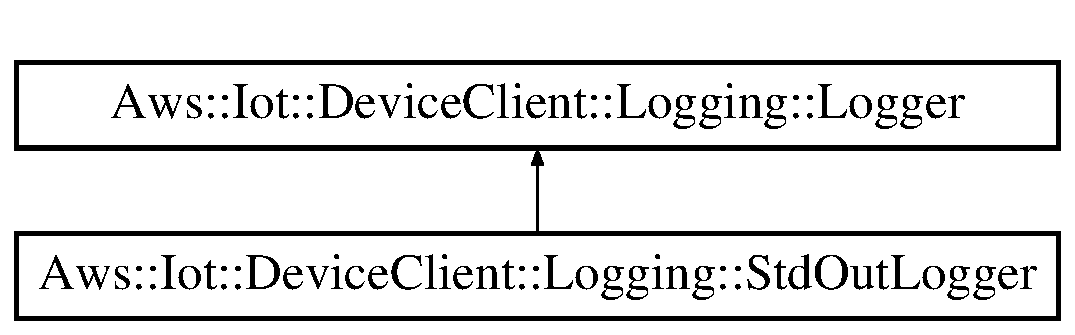
\includegraphics[height=2.000000cm]{class_aws_1_1_iot_1_1_device_client_1_1_logging_1_1_std_out_logger}
\end{center}
\end{figure}
\subsection*{Public Member Functions}
\begin{DoxyCompactItemize}
\item 
virtual bool \hyperlink{class_aws_1_1_iot_1_1_device_client_1_1_logging_1_1_std_out_logger_aa27086cd009717d85b957ef1740b14e9}{start} (const \hyperlink{struct_aws_1_1_iot_1_1_device_client_1_1_plain_config}{Plain\+Config} \&config) override
\begin{DoxyCompactList}\small\item\em Starts the underlying logger implementation\textquotesingle{}s logging behavior. \end{DoxyCompactList}\item 
\mbox{\Hypertarget{class_aws_1_1_iot_1_1_device_client_1_1_logging_1_1_std_out_logger_a1bf5765608b8109129488fe2bfa8616c}\label{class_aws_1_1_iot_1_1_device_client_1_1_logging_1_1_std_out_logger_a1bf5765608b8109129488fe2bfa8616c}} 
virtual void \hyperlink{class_aws_1_1_iot_1_1_device_client_1_1_logging_1_1_std_out_logger_a1bf5765608b8109129488fe2bfa8616c}{stop} () override
\begin{DoxyCompactList}\small\item\em Attempts to stop the \hyperlink{class_aws_1_1_iot_1_1_device_client_1_1_logging_1_1_logger}{Logger} implementation from writing any additional log messages, likely to switch to a different logger implementation. \end{DoxyCompactList}\item 
\mbox{\Hypertarget{class_aws_1_1_iot_1_1_device_client_1_1_logging_1_1_std_out_logger_ae0e55f2d2a1ce818ddb4ed14c293051f}\label{class_aws_1_1_iot_1_1_device_client_1_1_logging_1_1_std_out_logger_ae0e55f2d2a1ce818ddb4ed14c293051f}} 
virtual void \hyperlink{class_aws_1_1_iot_1_1_device_client_1_1_logging_1_1_std_out_logger_ae0e55f2d2a1ce818ddb4ed14c293051f}{shutdown} () override
\begin{DoxyCompactList}\small\item\em Notifies the \hyperlink{class_aws_1_1_iot_1_1_device_client_1_1_logging_1_1_logger}{Logger} implementation that any queued logs should be dumped to output and the logger should shut itself down. \end{DoxyCompactList}\item 
virtual std\+::unique\+\_\+ptr$<$ \hyperlink{class_aws_1_1_iot_1_1_device_client_1_1_logging_1_1_log_queue}{Log\+Queue} $>$ \hyperlink{class_aws_1_1_iot_1_1_device_client_1_1_logging_1_1_std_out_logger_acff57144a637686b21f27aa0da9628a2}{take\+Log\+Queue} () override
\begin{DoxyCompactList}\small\item\em Removes the \hyperlink{class_aws_1_1_iot_1_1_device_client_1_1_logging_1_1_log_queue}{Log\+Queue} from the logger implementation so it can be passed to another logger implementation for processing. \end{DoxyCompactList}\item 
virtual void \hyperlink{class_aws_1_1_iot_1_1_device_client_1_1_logging_1_1_std_out_logger_aa35c525dc9aa3fef0f1f244781d304ea}{set\+Log\+Queue} (std\+::unique\+\_\+ptr$<$ \hyperlink{class_aws_1_1_iot_1_1_device_client_1_1_logging_1_1_log_queue}{Log\+Queue} $>$ \hyperlink{class_aws_1_1_iot_1_1_device_client_1_1_logging_1_1_std_out_logger_a0c39b3bc0fa3164c5efc793fa54c58eb}{log\+Queue}) override
\begin{DoxyCompactList}\small\item\em Passes a \hyperlink{class_aws_1_1_iot_1_1_device_client_1_1_logging_1_1_log_queue}{Log\+Queue} to the logger implementation. Typically used if the logger implementation is being changed. \end{DoxyCompactList}\item 
virtual void \hyperlink{class_aws_1_1_iot_1_1_device_client_1_1_logging_1_1_std_out_logger_a27610c8adc232399266ef8c8f09eb46b}{flush} () override
\begin{DoxyCompactList}\small\item\em Flush the log output from the queue synchronously. \end{DoxyCompactList}\end{DoxyCompactItemize}
\subsection*{Protected Member Functions}
\begin{DoxyCompactItemize}
\item 
virtual void \hyperlink{class_aws_1_1_iot_1_1_device_client_1_1_logging_1_1_std_out_logger_a829dd9d573157d3cbc6865b38572dd85}{queue\+Log} (Log\+Level level, const char $\ast$tag, std\+::chrono\+::time\+\_\+point$<$ std\+::chrono\+::system\+\_\+clock $>$ t, std\+::string message) override
\begin{DoxyCompactList}\small\item\em Implemented by the underlying logger implementation to pass responsibility for managing the log message from the \hyperlink{class_aws_1_1_iot_1_1_device_client_1_1_logging_1_1_logger}{Logger} interface to the logger implementation. \end{DoxyCompactList}\end{DoxyCompactItemize}
\subsection*{Private Member Functions}
\begin{DoxyCompactItemize}
\item 
void \hyperlink{class_aws_1_1_iot_1_1_device_client_1_1_logging_1_1_std_out_logger_a8b7972522f4c1e399f9f8448da5703f5}{run} ()
\begin{DoxyCompactList}\small\item\em Begins processing of log messages in the \hyperlink{class_aws_1_1_iot_1_1_device_client_1_1_logging_1_1_log_queue}{Log\+Queue}. \end{DoxyCompactList}\item 
void \hyperlink{class_aws_1_1_iot_1_1_device_client_1_1_logging_1_1_std_out_logger_a795accad8a751b0f94341bb1b3325121}{write\+Log\+Message} (std\+::unique\+\_\+ptr$<$ \hyperlink{class_aws_1_1_iot_1_1_device_client_1_1_logging_1_1_log_message}{Log\+Message} $>$ message)
\begin{DoxyCompactList}\small\item\em Write the log message to standard output. \end{DoxyCompactList}\end{DoxyCompactItemize}
\subsection*{Private Attributes}
\begin{DoxyCompactItemize}
\item 
\mbox{\Hypertarget{class_aws_1_1_iot_1_1_device_client_1_1_logging_1_1_std_out_logger_a4e526296245920334c21e20e5cad0d75}\label{class_aws_1_1_iot_1_1_device_client_1_1_logging_1_1_std_out_logger_a4e526296245920334c21e20e5cad0d75}} 
bool \hyperlink{class_aws_1_1_iot_1_1_device_client_1_1_logging_1_1_std_out_logger_a4e526296245920334c21e20e5cad0d75}{needs\+Shutdown} = false
\begin{DoxyCompactList}\small\item\em Flag used to notify underlying threads that they should discontinue any processing so that the application can safely shutdown. \end{DoxyCompactList}\item 
\mbox{\Hypertarget{class_aws_1_1_iot_1_1_device_client_1_1_logging_1_1_std_out_logger_a0c39b3bc0fa3164c5efc793fa54c58eb}\label{class_aws_1_1_iot_1_1_device_client_1_1_logging_1_1_std_out_logger_a0c39b3bc0fa3164c5efc793fa54c58eb}} 
std\+::unique\+\_\+ptr$<$ \hyperlink{class_aws_1_1_iot_1_1_device_client_1_1_logging_1_1_log_queue}{Log\+Queue} $>$ \hyperlink{class_aws_1_1_iot_1_1_device_client_1_1_logging_1_1_std_out_logger_a0c39b3bc0fa3164c5efc793fa54c58eb}{log\+Queue} = std\+::unique\+\_\+ptr$<$\hyperlink{class_aws_1_1_iot_1_1_device_client_1_1_logging_1_1_log_queue}{Log\+Queue}$>$(new \hyperlink{class_aws_1_1_iot_1_1_device_client_1_1_logging_1_1_log_queue}{Log\+Queue})
\begin{DoxyCompactList}\small\item\em a \hyperlink{class_aws_1_1_iot_1_1_device_client_1_1_logging_1_1_log_queue}{Log\+Queue} instance used to queue incoming log messages for processing \end{DoxyCompactList}\end{DoxyCompactItemize}
\subsection*{Additional Inherited Members}


\subsection{Detailed Description}
Logging implementation that writes log messages directly to S\+T\+D\+O\+UT. 

\subsection{Member Function Documentation}
\mbox{\Hypertarget{class_aws_1_1_iot_1_1_device_client_1_1_logging_1_1_std_out_logger_a27610c8adc232399266ef8c8f09eb46b}\label{class_aws_1_1_iot_1_1_device_client_1_1_logging_1_1_std_out_logger_a27610c8adc232399266ef8c8f09eb46b}} 
\index{Aws\+::\+Iot\+::\+Device\+Client\+::\+Logging\+::\+Std\+Out\+Logger@{Aws\+::\+Iot\+::\+Device\+Client\+::\+Logging\+::\+Std\+Out\+Logger}!flush@{flush}}
\index{flush@{flush}!Aws\+::\+Iot\+::\+Device\+Client\+::\+Logging\+::\+Std\+Out\+Logger@{Aws\+::\+Iot\+::\+Device\+Client\+::\+Logging\+::\+Std\+Out\+Logger}}
\subsubsection{\texorpdfstring{flush()}{flush()}}
{\footnotesize\ttfamily void Std\+Out\+Logger\+::flush (\begin{DoxyParamCaption}{ }\end{DoxyParamCaption})\hspace{0.3cm}{\ttfamily [override]}, {\ttfamily [virtual]}}



Flush the log output from the queue synchronously. 

This is helpful for scenarios where you need to ensure that the logs are written to disk before any other activity takes place. Note that this will not block other threads, only the thread that this is called from 

Implements \hyperlink{class_aws_1_1_iot_1_1_device_client_1_1_logging_1_1_logger_a4743383e9c69bec10ba970dc4394781e}{Aws\+::\+Iot\+::\+Device\+Client\+::\+Logging\+::\+Logger}.

\mbox{\Hypertarget{class_aws_1_1_iot_1_1_device_client_1_1_logging_1_1_std_out_logger_a829dd9d573157d3cbc6865b38572dd85}\label{class_aws_1_1_iot_1_1_device_client_1_1_logging_1_1_std_out_logger_a829dd9d573157d3cbc6865b38572dd85}} 
\index{Aws\+::\+Iot\+::\+Device\+Client\+::\+Logging\+::\+Std\+Out\+Logger@{Aws\+::\+Iot\+::\+Device\+Client\+::\+Logging\+::\+Std\+Out\+Logger}!queue\+Log@{queue\+Log}}
\index{queue\+Log@{queue\+Log}!Aws\+::\+Iot\+::\+Device\+Client\+::\+Logging\+::\+Std\+Out\+Logger@{Aws\+::\+Iot\+::\+Device\+Client\+::\+Logging\+::\+Std\+Out\+Logger}}
\subsubsection{\texorpdfstring{queue\+Log()}{queueLog()}}
{\footnotesize\ttfamily void Std\+Out\+Logger\+::queue\+Log (\begin{DoxyParamCaption}\item[{Log\+Level}]{level,  }\item[{const char $\ast$}]{tag,  }\item[{std\+::chrono\+::time\+\_\+point$<$ std\+::chrono\+::system\+\_\+clock $>$}]{t,  }\item[{std\+::string}]{message }\end{DoxyParamCaption})\hspace{0.3cm}{\ttfamily [override]}, {\ttfamily [protected]}, {\ttfamily [virtual]}}



Implemented by the underlying logger implementation to pass responsibility for managing the log message from the \hyperlink{class_aws_1_1_iot_1_1_device_client_1_1_logging_1_1_logger}{Logger} interface to the logger implementation. 

This virtual method should be implemented by the underlying logger implementation to actually accept and eventually process the incoming log message. To reduce complications induced by multithreading, the underlying logger implementation should queue the message for processing by another thread if possible. 
\begin{DoxyParams}{Parameters}
{\em level} & the log level \\
\hline
{\em tag} & a tag that indicates where the log message is coming from \\
\hline
{\em t} & a timestamp representing the time the message was created \\
\hline
{\em message} & the message to log \\
\hline
\end{DoxyParams}


Implements \hyperlink{class_aws_1_1_iot_1_1_device_client_1_1_logging_1_1_logger_a75acdae576e13ddd84bccb70d8fb1fef}{Aws\+::\+Iot\+::\+Device\+Client\+::\+Logging\+::\+Logger}.

\mbox{\Hypertarget{class_aws_1_1_iot_1_1_device_client_1_1_logging_1_1_std_out_logger_a8b7972522f4c1e399f9f8448da5703f5}\label{class_aws_1_1_iot_1_1_device_client_1_1_logging_1_1_std_out_logger_a8b7972522f4c1e399f9f8448da5703f5}} 
\index{Aws\+::\+Iot\+::\+Device\+Client\+::\+Logging\+::\+Std\+Out\+Logger@{Aws\+::\+Iot\+::\+Device\+Client\+::\+Logging\+::\+Std\+Out\+Logger}!run@{run}}
\index{run@{run}!Aws\+::\+Iot\+::\+Device\+Client\+::\+Logging\+::\+Std\+Out\+Logger@{Aws\+::\+Iot\+::\+Device\+Client\+::\+Logging\+::\+Std\+Out\+Logger}}
\subsubsection{\texorpdfstring{run()}{run()}}
{\footnotesize\ttfamily void Std\+Out\+Logger\+::run (\begin{DoxyParamCaption}{ }\end{DoxyParamCaption})\hspace{0.3cm}{\ttfamily [private]}}



Begins processing of log messages in the \hyperlink{class_aws_1_1_iot_1_1_device_client_1_1_logging_1_1_log_queue}{Log\+Queue}. 

This method will begin processing of log messages in the \hyperlink{class_aws_1_1_iot_1_1_device_client_1_1_logging_1_1_log_queue}{Log\+Queue}. The thread will process until all of the messages are removed from the queue, and then will wait until new messages arrive in the queue. This method will check to make sure the \hyperlink{class_aws_1_1_iot_1_1_device_client_1_1_logging_1_1_std_out_logger_ae0e55f2d2a1ce818ddb4ed14c293051f}{shutdown()} method has not been called before processing any additional messages in the queue. \mbox{\Hypertarget{class_aws_1_1_iot_1_1_device_client_1_1_logging_1_1_std_out_logger_aa35c525dc9aa3fef0f1f244781d304ea}\label{class_aws_1_1_iot_1_1_device_client_1_1_logging_1_1_std_out_logger_aa35c525dc9aa3fef0f1f244781d304ea}} 
\index{Aws\+::\+Iot\+::\+Device\+Client\+::\+Logging\+::\+Std\+Out\+Logger@{Aws\+::\+Iot\+::\+Device\+Client\+::\+Logging\+::\+Std\+Out\+Logger}!set\+Log\+Queue@{set\+Log\+Queue}}
\index{set\+Log\+Queue@{set\+Log\+Queue}!Aws\+::\+Iot\+::\+Device\+Client\+::\+Logging\+::\+Std\+Out\+Logger@{Aws\+::\+Iot\+::\+Device\+Client\+::\+Logging\+::\+Std\+Out\+Logger}}
\subsubsection{\texorpdfstring{set\+Log\+Queue()}{setLogQueue()}}
{\footnotesize\ttfamily void Std\+Out\+Logger\+::set\+Log\+Queue (\begin{DoxyParamCaption}\item[{std\+::unique\+\_\+ptr$<$ \hyperlink{class_aws_1_1_iot_1_1_device_client_1_1_logging_1_1_log_queue}{Log\+Queue} $>$}]{log\+Queue }\end{DoxyParamCaption})\hspace{0.3cm}{\ttfamily [override]}, {\ttfamily [virtual]}}



Passes a \hyperlink{class_aws_1_1_iot_1_1_device_client_1_1_logging_1_1_log_queue}{Log\+Queue} to the logger implementation. Typically used if the logger implementation is being changed. 


\begin{DoxyParams}{Parameters}
{\em log\+Queue} & \\
\hline
\end{DoxyParams}


Implements \hyperlink{class_aws_1_1_iot_1_1_device_client_1_1_logging_1_1_logger_a6b80ca4200fbc58bb2994ef4319ea822}{Aws\+::\+Iot\+::\+Device\+Client\+::\+Logging\+::\+Logger}.

\mbox{\Hypertarget{class_aws_1_1_iot_1_1_device_client_1_1_logging_1_1_std_out_logger_aa27086cd009717d85b957ef1740b14e9}\label{class_aws_1_1_iot_1_1_device_client_1_1_logging_1_1_std_out_logger_aa27086cd009717d85b957ef1740b14e9}} 
\index{Aws\+::\+Iot\+::\+Device\+Client\+::\+Logging\+::\+Std\+Out\+Logger@{Aws\+::\+Iot\+::\+Device\+Client\+::\+Logging\+::\+Std\+Out\+Logger}!start@{start}}
\index{start@{start}!Aws\+::\+Iot\+::\+Device\+Client\+::\+Logging\+::\+Std\+Out\+Logger@{Aws\+::\+Iot\+::\+Device\+Client\+::\+Logging\+::\+Std\+Out\+Logger}}
\subsubsection{\texorpdfstring{start()}{start()}}
{\footnotesize\ttfamily bool Std\+Out\+Logger\+::start (\begin{DoxyParamCaption}\item[{const \hyperlink{struct_aws_1_1_iot_1_1_device_client_1_1_plain_config}{Plain\+Config} \&}]{config }\end{DoxyParamCaption})\hspace{0.3cm}{\ttfamily [override]}, {\ttfamily [virtual]}}



Starts the underlying logger implementation\textquotesingle{}s logging behavior. 


\begin{DoxyParams}{Parameters}
{\em config} & the config data passed in from the C\+LI and J\+S\+ON \\
\hline
\end{DoxyParams}
\begin{DoxyReturn}{Returns}
true if it is able to start successfully, false otherwise 
\end{DoxyReturn}


Implements \hyperlink{class_aws_1_1_iot_1_1_device_client_1_1_logging_1_1_logger_ad42e38afcd7402f5dc1213b2f0b96961}{Aws\+::\+Iot\+::\+Device\+Client\+::\+Logging\+::\+Logger}.

\mbox{\Hypertarget{class_aws_1_1_iot_1_1_device_client_1_1_logging_1_1_std_out_logger_acff57144a637686b21f27aa0da9628a2}\label{class_aws_1_1_iot_1_1_device_client_1_1_logging_1_1_std_out_logger_acff57144a637686b21f27aa0da9628a2}} 
\index{Aws\+::\+Iot\+::\+Device\+Client\+::\+Logging\+::\+Std\+Out\+Logger@{Aws\+::\+Iot\+::\+Device\+Client\+::\+Logging\+::\+Std\+Out\+Logger}!take\+Log\+Queue@{take\+Log\+Queue}}
\index{take\+Log\+Queue@{take\+Log\+Queue}!Aws\+::\+Iot\+::\+Device\+Client\+::\+Logging\+::\+Std\+Out\+Logger@{Aws\+::\+Iot\+::\+Device\+Client\+::\+Logging\+::\+Std\+Out\+Logger}}
\subsubsection{\texorpdfstring{take\+Log\+Queue()}{takeLogQueue()}}
{\footnotesize\ttfamily unique\+\_\+ptr$<$ \hyperlink{class_aws_1_1_iot_1_1_device_client_1_1_logging_1_1_log_queue}{Log\+Queue} $>$ Std\+Out\+Logger\+::take\+Log\+Queue (\begin{DoxyParamCaption}{ }\end{DoxyParamCaption})\hspace{0.3cm}{\ttfamily [override]}, {\ttfamily [virtual]}}



Removes the \hyperlink{class_aws_1_1_iot_1_1_device_client_1_1_logging_1_1_log_queue}{Log\+Queue} from the logger implementation so it can be passed to another logger implementation for processing. 

\begin{DoxyReturn}{Returns}
a unique\+\_\+ptr$<$\+Log\+Queue$>$ 
\end{DoxyReturn}


Implements \hyperlink{class_aws_1_1_iot_1_1_device_client_1_1_logging_1_1_logger_a39f3326be17f9ed4b1385f057134774d}{Aws\+::\+Iot\+::\+Device\+Client\+::\+Logging\+::\+Logger}.

\mbox{\Hypertarget{class_aws_1_1_iot_1_1_device_client_1_1_logging_1_1_std_out_logger_a795accad8a751b0f94341bb1b3325121}\label{class_aws_1_1_iot_1_1_device_client_1_1_logging_1_1_std_out_logger_a795accad8a751b0f94341bb1b3325121}} 
\index{Aws\+::\+Iot\+::\+Device\+Client\+::\+Logging\+::\+Std\+Out\+Logger@{Aws\+::\+Iot\+::\+Device\+Client\+::\+Logging\+::\+Std\+Out\+Logger}!write\+Log\+Message@{write\+Log\+Message}}
\index{write\+Log\+Message@{write\+Log\+Message}!Aws\+::\+Iot\+::\+Device\+Client\+::\+Logging\+::\+Std\+Out\+Logger@{Aws\+::\+Iot\+::\+Device\+Client\+::\+Logging\+::\+Std\+Out\+Logger}}
\subsubsection{\texorpdfstring{write\+Log\+Message()}{writeLogMessage()}}
{\footnotesize\ttfamily void Std\+Out\+Logger\+::write\+Log\+Message (\begin{DoxyParamCaption}\item[{std\+::unique\+\_\+ptr$<$ \hyperlink{class_aws_1_1_iot_1_1_device_client_1_1_logging_1_1_log_message}{Log\+Message} $>$}]{message }\end{DoxyParamCaption})\hspace{0.3cm}{\ttfamily [private]}}



Write the log message to standard output. 

This method will write the log message to the file specified for logging 
\begin{DoxyParams}{Parameters}
{\em message} & the message to log \\
\hline
\end{DoxyParams}


The documentation for this class was generated from the following files\+:\begin{DoxyCompactItemize}
\item 
/home/\+A\+N\+T.\+A\+M\+A\+Z\+O\+N.\+C\+O\+M/lwwilkov/\+Workspace/aws-\/iot-\/device-\/client/source/logging/Std\+Out\+Logger.\+h\item 
/home/\+A\+N\+T.\+A\+M\+A\+Z\+O\+N.\+C\+O\+M/lwwilkov/\+Workspace/aws-\/iot-\/device-\/client/source/logging/Std\+Out\+Logger.\+cpp\end{DoxyCompactItemize}

\hypertarget{class_aws_1_1_iot_1_1_device_client_1_1_secure_tunneling_1_1_tcp_forward}{}\doxysection{Aws\+::Iot\+::Device\+Client\+::Secure\+Tunneling\+::Tcp\+Forward Class Reference}
\label{class_aws_1_1_iot_1_1_device_client_1_1_secure_tunneling_1_1_tcp_forward}\index{Aws::Iot::DeviceClient::SecureTunneling::TcpForward@{Aws::Iot::DeviceClient::SecureTunneling::TcpForward}}


A class that represents a local T\+CP socket. It implements all callbacks required by using aws\+\_\+socket.  




{\ttfamily \#include $<$Tcp\+Forward.\+h$>$}

\doxysubsection*{Public Member Functions}
\begin{DoxyCompactItemize}
\item 
\mbox{\hyperlink{class_aws_1_1_iot_1_1_device_client_1_1_secure_tunneling_1_1_tcp_forward_ab7c56677f6f28b12223830a238bd9a17}{Tcp\+Forward}} (std\+::shared\+\_\+ptr$<$ \mbox{\hyperlink{class_aws_1_1_iot_1_1_device_client_1_1_shared_crt_resource_manager}{Shared\+Crt\+Resource\+Manager}} $>$ shared\+Crt\+Resource\+Manager, uint16\+\_\+t port, On\+Tcp\+Forward\+Data\+Receive on\+Tcp\+Forward\+Data\+Receive)
\begin{DoxyCompactList}\small\item\em Constructor. \end{DoxyCompactList}\item 
\mbox{\Hypertarget{class_aws_1_1_iot_1_1_device_client_1_1_secure_tunneling_1_1_tcp_forward_a5c893165a638399f815c7889d66096f6}\label{class_aws_1_1_iot_1_1_device_client_1_1_secure_tunneling_1_1_tcp_forward_a5c893165a638399f815c7889d66096f6}} 
\mbox{\hyperlink{class_aws_1_1_iot_1_1_device_client_1_1_secure_tunneling_1_1_tcp_forward_a5c893165a638399f815c7889d66096f6}{$\sim$\+Tcp\+Forward}} ()
\begin{DoxyCompactList}\small\item\em Destructor. \end{DoxyCompactList}\item 
\mbox{\Hypertarget{class_aws_1_1_iot_1_1_device_client_1_1_secure_tunneling_1_1_tcp_forward_a13b963b1009718b84b79e7b2943792a5}\label{class_aws_1_1_iot_1_1_device_client_1_1_secure_tunneling_1_1_tcp_forward_a13b963b1009718b84b79e7b2943792a5}} 
int \mbox{\hyperlink{class_aws_1_1_iot_1_1_device_client_1_1_secure_tunneling_1_1_tcp_forward_a13b963b1009718b84b79e7b2943792a5}{Connect}} ()
\begin{DoxyCompactList}\small\item\em Connect to the local T\+CP socket. \end{DoxyCompactList}\item 
\mbox{\Hypertarget{class_aws_1_1_iot_1_1_device_client_1_1_secure_tunneling_1_1_tcp_forward_af0961f83e2e761252a7560616f927593}\label{class_aws_1_1_iot_1_1_device_client_1_1_secure_tunneling_1_1_tcp_forward_af0961f83e2e761252a7560616f927593}} 
int \mbox{\hyperlink{class_aws_1_1_iot_1_1_device_client_1_1_secure_tunneling_1_1_tcp_forward_af0961f83e2e761252a7560616f927593}{Close}} ()
\begin{DoxyCompactList}\small\item\em Close the local T\+CP socket. \end{DoxyCompactList}\item 
int \mbox{\hyperlink{class_aws_1_1_iot_1_1_device_client_1_1_secure_tunneling_1_1_tcp_forward_aa20aab4ae6ecd3004100da9976b95310}{Send\+Data}} (const Crt\+::\+Byte\+Cursor \&data)
\begin{DoxyCompactList}\small\item\em Send the given payload to the T\+CP socket. \end{DoxyCompactList}\end{DoxyCompactItemize}
\doxysubsection*{Private Member Functions}
\begin{DoxyCompactItemize}
\item 
\mbox{\Hypertarget{class_aws_1_1_iot_1_1_device_client_1_1_secure_tunneling_1_1_tcp_forward_a1c0858f85b387468dd56715ffdf9ee92}\label{class_aws_1_1_iot_1_1_device_client_1_1_secure_tunneling_1_1_tcp_forward_a1c0858f85b387468dd56715ffdf9ee92}} 
void \mbox{\hyperlink{class_aws_1_1_iot_1_1_device_client_1_1_secure_tunneling_1_1_tcp_forward_a1c0858f85b387468dd56715ffdf9ee92}{On\+Connection\+Result}} (struct aws\+\_\+socket $\ast$socket, int error\+\_\+code)
\begin{DoxyCompactList}\small\item\em Callback when connection to a socket is complete. \end{DoxyCompactList}\item 
\mbox{\Hypertarget{class_aws_1_1_iot_1_1_device_client_1_1_secure_tunneling_1_1_tcp_forward_ae2d1c879f7f37bdfe7a965ad6736b7df}\label{class_aws_1_1_iot_1_1_device_client_1_1_secure_tunneling_1_1_tcp_forward_ae2d1c879f7f37bdfe7a965ad6736b7df}} 
void \mbox{\hyperlink{class_aws_1_1_iot_1_1_device_client_1_1_secure_tunneling_1_1_tcp_forward_ae2d1c879f7f37bdfe7a965ad6736b7df}{On\+Write\+Completed}} (struct aws\+\_\+socket $\ast$socket, int error\+\_\+code, size\+\_\+t bytes\+\_\+written)
\begin{DoxyCompactList}\small\item\em Callback when writing to the socket is complete. \end{DoxyCompactList}\item 
\mbox{\Hypertarget{class_aws_1_1_iot_1_1_device_client_1_1_secure_tunneling_1_1_tcp_forward_a60a65f8be68d2008bf5410657e4624ff}\label{class_aws_1_1_iot_1_1_device_client_1_1_secure_tunneling_1_1_tcp_forward_a60a65f8be68d2008bf5410657e4624ff}} 
void \mbox{\hyperlink{class_aws_1_1_iot_1_1_device_client_1_1_secure_tunneling_1_1_tcp_forward_a60a65f8be68d2008bf5410657e4624ff}{On\+Readable}} (struct aws\+\_\+socket $\ast$socket, int error\+\_\+code)
\begin{DoxyCompactList}\small\item\em Callback when the socket has data to read. \end{DoxyCompactList}\item 
\mbox{\Hypertarget{class_aws_1_1_iot_1_1_device_client_1_1_secure_tunneling_1_1_tcp_forward_a702830a3834fd824dc013be4c9f355f9}\label{class_aws_1_1_iot_1_1_device_client_1_1_secure_tunneling_1_1_tcp_forward_a702830a3834fd824dc013be4c9f355f9}} 
void \mbox{\hyperlink{class_aws_1_1_iot_1_1_device_client_1_1_secure_tunneling_1_1_tcp_forward_a702830a3834fd824dc013be4c9f355f9}{Flush\+Send\+Buffer}} ()
\begin{DoxyCompactList}\small\item\em Flush any buffered data (saved before the socket is ready) to the socket. \end{DoxyCompactList}\end{DoxyCompactItemize}
\doxysubsection*{Static Private Member Functions}
\begin{DoxyCompactItemize}
\item 
\mbox{\Hypertarget{class_aws_1_1_iot_1_1_device_client_1_1_secure_tunneling_1_1_tcp_forward_a04d36587c626df9c2392fd2f3ff12122}\label{class_aws_1_1_iot_1_1_device_client_1_1_secure_tunneling_1_1_tcp_forward_a04d36587c626df9c2392fd2f3ff12122}} 
static void \mbox{\hyperlink{class_aws_1_1_iot_1_1_device_client_1_1_secure_tunneling_1_1_tcp_forward_a04d36587c626df9c2392fd2f3ff12122}{s\+On\+Connection\+Result}} (struct aws\+\_\+socket $\ast$socket, int error\+\_\+code, void $\ast$user\+\_\+data)
\begin{DoxyCompactList}\small\item\em Callback when connection to a socket is complete. \end{DoxyCompactList}\item 
\mbox{\Hypertarget{class_aws_1_1_iot_1_1_device_client_1_1_secure_tunneling_1_1_tcp_forward_a4203de375f36fbde339599d435b511b0}\label{class_aws_1_1_iot_1_1_device_client_1_1_secure_tunneling_1_1_tcp_forward_a4203de375f36fbde339599d435b511b0}} 
static void \mbox{\hyperlink{class_aws_1_1_iot_1_1_device_client_1_1_secure_tunneling_1_1_tcp_forward_a4203de375f36fbde339599d435b511b0}{s\+On\+Write\+Completed}} (struct aws\+\_\+socket $\ast$socket, int error\+\_\+code, size\+\_\+t bytes\+\_\+written, void $\ast$user\+\_\+data)
\begin{DoxyCompactList}\small\item\em Callback when writing to the socket is complete. \end{DoxyCompactList}\item 
\mbox{\Hypertarget{class_aws_1_1_iot_1_1_device_client_1_1_secure_tunneling_1_1_tcp_forward_a59535904825ea855774f41f880f0c778}\label{class_aws_1_1_iot_1_1_device_client_1_1_secure_tunneling_1_1_tcp_forward_a59535904825ea855774f41f880f0c778}} 
static void \mbox{\hyperlink{class_aws_1_1_iot_1_1_device_client_1_1_secure_tunneling_1_1_tcp_forward_a59535904825ea855774f41f880f0c778}{s\+On\+Readable}} (struct aws\+\_\+socket $\ast$socket, int error\+\_\+code, void $\ast$user\+\_\+data)
\begin{DoxyCompactList}\small\item\em Callback when the socket has data to read. \end{DoxyCompactList}\end{DoxyCompactItemize}
\doxysubsection*{Private Attributes}
\begin{DoxyCompactItemize}
\item 
\mbox{\Hypertarget{class_aws_1_1_iot_1_1_device_client_1_1_secure_tunneling_1_1_tcp_forward_a6f68f3a182d517fed7376e8874207b7a}\label{class_aws_1_1_iot_1_1_device_client_1_1_secure_tunneling_1_1_tcp_forward_a6f68f3a182d517fed7376e8874207b7a}} 
std\+::shared\+\_\+ptr$<$ \mbox{\hyperlink{class_aws_1_1_iot_1_1_device_client_1_1_shared_crt_resource_manager}{Shared\+Crt\+Resource\+Manager}} $>$ \mbox{\hyperlink{class_aws_1_1_iot_1_1_device_client_1_1_secure_tunneling_1_1_tcp_forward_a6f68f3a182d517fed7376e8874207b7a}{m\+Shared\+Crt\+Resource\+Manager}}
\begin{DoxyCompactList}\small\item\em The resource manager used to manage C\+RT resources. \end{DoxyCompactList}\item 
\mbox{\Hypertarget{class_aws_1_1_iot_1_1_device_client_1_1_secure_tunneling_1_1_tcp_forward_a991b1bb00f6389f3a9e49984c09cfd18}\label{class_aws_1_1_iot_1_1_device_client_1_1_secure_tunneling_1_1_tcp_forward_a991b1bb00f6389f3a9e49984c09cfd18}} 
uint16\+\_\+t \mbox{\hyperlink{class_aws_1_1_iot_1_1_device_client_1_1_secure_tunneling_1_1_tcp_forward_a991b1bb00f6389f3a9e49984c09cfd18}{m\+Port}}
\begin{DoxyCompactList}\small\item\em The local T\+CP port to connect to. \end{DoxyCompactList}\item 
\mbox{\Hypertarget{class_aws_1_1_iot_1_1_device_client_1_1_secure_tunneling_1_1_tcp_forward_a7260f7982d221b29480ab16092505b2e}\label{class_aws_1_1_iot_1_1_device_client_1_1_secure_tunneling_1_1_tcp_forward_a7260f7982d221b29480ab16092505b2e}} 
On\+Tcp\+Forward\+Data\+Receive \mbox{\hyperlink{class_aws_1_1_iot_1_1_device_client_1_1_secure_tunneling_1_1_tcp_forward_a7260f7982d221b29480ab16092505b2e}{m\+On\+Tcp\+Forward\+Data\+Receive}}
\begin{DoxyCompactList}\small\item\em Callback when data is received from the local T\+CP port. \end{DoxyCompactList}\item 
\mbox{\Hypertarget{class_aws_1_1_iot_1_1_device_client_1_1_secure_tunneling_1_1_tcp_forward_a624e8376d97bd12aa650e3cd018efd7a}\label{class_aws_1_1_iot_1_1_device_client_1_1_secure_tunneling_1_1_tcp_forward_a624e8376d97bd12aa650e3cd018efd7a}} 
aws\+\_\+socket \mbox{\hyperlink{class_aws_1_1_iot_1_1_device_client_1_1_secure_tunneling_1_1_tcp_forward_a624e8376d97bd12aa650e3cd018efd7a}{m\+Socket}} \{\}
\begin{DoxyCompactList}\small\item\em An A\+WS S\+DK socket object. It manages the connection to the local T\+CP port. \end{DoxyCompactList}\item 
\mbox{\Hypertarget{class_aws_1_1_iot_1_1_device_client_1_1_secure_tunneling_1_1_tcp_forward_a899ca18e84f5f14bac91ae77b26dc41f}\label{class_aws_1_1_iot_1_1_device_client_1_1_secure_tunneling_1_1_tcp_forward_a899ca18e84f5f14bac91ae77b26dc41f}} 
bool \mbox{\hyperlink{class_aws_1_1_iot_1_1_device_client_1_1_secure_tunneling_1_1_tcp_forward_a899ca18e84f5f14bac91ae77b26dc41f}{m\+Connected}}
\begin{DoxyCompactList}\small\item\em Is the socket connected yet? \end{DoxyCompactList}\item 
\mbox{\Hypertarget{class_aws_1_1_iot_1_1_device_client_1_1_secure_tunneling_1_1_tcp_forward_a6efb4ad2b675389b667621c154cb5b54}\label{class_aws_1_1_iot_1_1_device_client_1_1_secure_tunneling_1_1_tcp_forward_a6efb4ad2b675389b667621c154cb5b54}} 
Aws\+::\+Crt\+::\+Byte\+Buf \mbox{\hyperlink{class_aws_1_1_iot_1_1_device_client_1_1_secure_tunneling_1_1_tcp_forward_a6efb4ad2b675389b667621c154cb5b54}{m\+Send\+Buffer}}
\begin{DoxyCompactList}\small\item\em A buffer to store data from the secure tunnel. This is only used before the socket is connected. \end{DoxyCompactList}\end{DoxyCompactItemize}
\doxysubsection*{Static Private Attributes}
\begin{DoxyCompactItemize}
\item 
\mbox{\Hypertarget{class_aws_1_1_iot_1_1_device_client_1_1_secure_tunneling_1_1_tcp_forward_a2a696885fdeba14f64b09781b2275ab5}\label{class_aws_1_1_iot_1_1_device_client_1_1_secure_tunneling_1_1_tcp_forward_a2a696885fdeba14f64b09781b2275ab5}} 
static constexpr char \mbox{\hyperlink{class_aws_1_1_iot_1_1_device_client_1_1_secure_tunneling_1_1_tcp_forward_a2a696885fdeba14f64b09781b2275ab5}{T\+AG}} \mbox{[}$\,$\mbox{]} = \char`\"{}Tcp\+Forward.\+cpp\char`\"{}
\begin{DoxyCompactList}\small\item\em Used by the logger to specify that log messages are coming from this class. \end{DoxyCompactList}\end{DoxyCompactItemize}


\doxysubsection{Detailed Description}
A class that represents a local T\+CP socket. It implements all callbacks required by using aws\+\_\+socket. 

\doxysubsection{Constructor \& Destructor Documentation}
\mbox{\Hypertarget{class_aws_1_1_iot_1_1_device_client_1_1_secure_tunneling_1_1_tcp_forward_ab7c56677f6f28b12223830a238bd9a17}\label{class_aws_1_1_iot_1_1_device_client_1_1_secure_tunneling_1_1_tcp_forward_ab7c56677f6f28b12223830a238bd9a17}} 
\index{Aws::Iot::DeviceClient::SecureTunneling::TcpForward@{Aws::Iot::DeviceClient::SecureTunneling::TcpForward}!TcpForward@{TcpForward}}
\index{TcpForward@{TcpForward}!Aws::Iot::DeviceClient::SecureTunneling::TcpForward@{Aws::Iot::DeviceClient::SecureTunneling::TcpForward}}
\doxysubsubsection{\texorpdfstring{TcpForward()}{TcpForward()}}
{\footnotesize\ttfamily Aws\+::\+Iot\+::\+Device\+Client\+::\+Secure\+Tunneling\+::\+Tcp\+Forward\+::\+Tcp\+Forward (\begin{DoxyParamCaption}\item[{std\+::shared\+\_\+ptr$<$ \mbox{\hyperlink{class_aws_1_1_iot_1_1_device_client_1_1_shared_crt_resource_manager}{Shared\+Crt\+Resource\+Manager}} $>$}]{shared\+Crt\+Resource\+Manager,  }\item[{uint16\+\_\+t}]{port,  }\item[{On\+Tcp\+Forward\+Data\+Receive}]{on\+Tcp\+Forward\+Data\+Receive }\end{DoxyParamCaption})}



Constructor. 


\begin{DoxyParams}{Parameters}
{\em shared\+Crt\+Resource\+Manager} & the shared resource manager \\
\hline
{\em port} & the local T\+CP port to connect to \\
\hline
{\em on\+Tcp\+Forward\+Data\+Receive} & callback when there is data received from the local T\+CP port \\
\hline
\end{DoxyParams}


\doxysubsection{Member Function Documentation}
\mbox{\Hypertarget{class_aws_1_1_iot_1_1_device_client_1_1_secure_tunneling_1_1_tcp_forward_aa20aab4ae6ecd3004100da9976b95310}\label{class_aws_1_1_iot_1_1_device_client_1_1_secure_tunneling_1_1_tcp_forward_aa20aab4ae6ecd3004100da9976b95310}} 
\index{Aws::Iot::DeviceClient::SecureTunneling::TcpForward@{Aws::Iot::DeviceClient::SecureTunneling::TcpForward}!SendData@{SendData}}
\index{SendData@{SendData}!Aws::Iot::DeviceClient::SecureTunneling::TcpForward@{Aws::Iot::DeviceClient::SecureTunneling::TcpForward}}
\doxysubsubsection{\texorpdfstring{SendData()}{SendData()}}
{\footnotesize\ttfamily int Aws\+::\+Iot\+::\+Device\+Client\+::\+Secure\+Tunneling\+::\+Tcp\+Forward\+::\+Send\+Data (\begin{DoxyParamCaption}\item[{const Crt\+::\+Byte\+Cursor \&}]{data }\end{DoxyParamCaption})}



Send the given payload to the T\+CP socket. 


\begin{DoxyParams}{Parameters}
{\em data} & the payload to send \\
\hline
\end{DoxyParams}


The documentation for this class was generated from the following files\+:\begin{DoxyCompactItemize}
\item 
/home/runner/work/aws-\/iot-\/device-\/client/aws-\/iot-\/device-\/client/source/tunneling/Tcp\+Forward.\+h\item 
/home/runner/work/aws-\/iot-\/device-\/client/aws-\/iot-\/device-\/client/source/tunneling/Tcp\+Forward.\+cpp\end{DoxyCompactItemize}

\hypertarget{struct_aws_1_1_iot_1_1_device_client_1_1_plain_config_1_1_tunneling}{}\section{Aws\+:\+:Iot\+:\+:Device\+Client\+:\+:Plain\+Config\+:\+:Tunneling Struct Reference}
\label{struct_aws_1_1_iot_1_1_device_client_1_1_plain_config_1_1_tunneling}\index{Aws\+::\+Iot\+::\+Device\+Client\+::\+Plain\+Config\+::\+Tunneling@{Aws\+::\+Iot\+::\+Device\+Client\+::\+Plain\+Config\+::\+Tunneling}}
Inheritance diagram for Aws\+:\+:Iot\+:\+:Device\+Client\+:\+:Plain\+Config\+:\+:Tunneling\+:\begin{figure}[H]
\begin{center}
\leavevmode
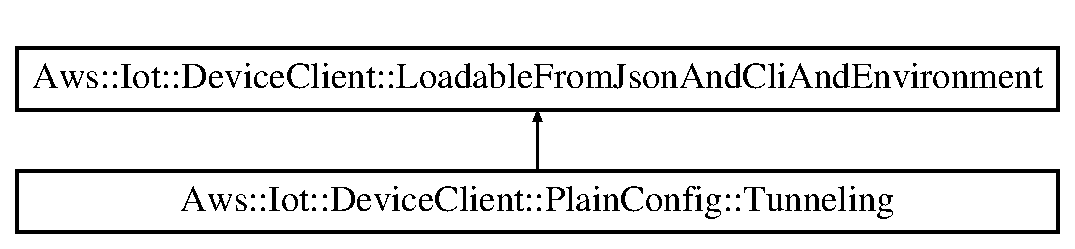
\includegraphics[height=2.000000cm]{struct_aws_1_1_iot_1_1_device_client_1_1_plain_config_1_1_tunneling}
\end{center}
\end{figure}
\subsection*{Public Member Functions}
\begin{DoxyCompactItemize}
\item 
\mbox{\Hypertarget{struct_aws_1_1_iot_1_1_device_client_1_1_plain_config_1_1_tunneling_a561dfb1259926bfe31d8c03bad4eef7d}\label{struct_aws_1_1_iot_1_1_device_client_1_1_plain_config_1_1_tunneling_a561dfb1259926bfe31d8c03bad4eef7d}} 
bool {\bfseries Load\+From\+Json} (const Crt\+::\+Json\+View \&json) override
\item 
\mbox{\Hypertarget{struct_aws_1_1_iot_1_1_device_client_1_1_plain_config_1_1_tunneling_ad5321178f74957eef3c6a91f1b3dbb7b}\label{struct_aws_1_1_iot_1_1_device_client_1_1_plain_config_1_1_tunneling_ad5321178f74957eef3c6a91f1b3dbb7b}} 
bool {\bfseries Load\+From\+Cli\+Args} (const Cli\+Args \&cli\+Args) override
\item 
\mbox{\Hypertarget{struct_aws_1_1_iot_1_1_device_client_1_1_plain_config_1_1_tunneling_aa4b606a5192cba3a72300ea1bc62b791}\label{struct_aws_1_1_iot_1_1_device_client_1_1_plain_config_1_1_tunneling_aa4b606a5192cba3a72300ea1bc62b791}} 
bool {\bfseries Load\+From\+Environment} () override
\item 
\mbox{\Hypertarget{struct_aws_1_1_iot_1_1_device_client_1_1_plain_config_1_1_tunneling_a90ec2cff99ff6fb0bb0e50aaa48bb42b}\label{struct_aws_1_1_iot_1_1_device_client_1_1_plain_config_1_1_tunneling_a90ec2cff99ff6fb0bb0e50aaa48bb42b}} 
bool {\bfseries Validate} () const override
\end{DoxyCompactItemize}
\subsection*{Public Attributes}
\begin{DoxyCompactItemize}
\item 
\mbox{\Hypertarget{struct_aws_1_1_iot_1_1_device_client_1_1_plain_config_1_1_tunneling_a6a6d6e957f99f27309f6fc1e51590bf0}\label{struct_aws_1_1_iot_1_1_device_client_1_1_plain_config_1_1_tunneling_a6a6d6e957f99f27309f6fc1e51590bf0}} 
bool {\bfseries enabled} \{true\}
\item 
\mbox{\Hypertarget{struct_aws_1_1_iot_1_1_device_client_1_1_plain_config_1_1_tunneling_a100273d25fa8b1664367785219f3dbfb}\label{struct_aws_1_1_iot_1_1_device_client_1_1_plain_config_1_1_tunneling_a100273d25fa8b1664367785219f3dbfb}} 
bool {\bfseries subscribe\+Notification} \{true\}
\item 
\mbox{\Hypertarget{struct_aws_1_1_iot_1_1_device_client_1_1_plain_config_1_1_tunneling_a29ab11ae97d402a20660154ba24e8b02}\label{struct_aws_1_1_iot_1_1_device_client_1_1_plain_config_1_1_tunneling_a29ab11ae97d402a20660154ba24e8b02}} 
Aws\+::\+Crt\+::\+Optional$<$ std\+::string $>$ {\bfseries destination\+Access\+Token}
\item 
\mbox{\Hypertarget{struct_aws_1_1_iot_1_1_device_client_1_1_plain_config_1_1_tunneling_a32c9bd2a50d6d2a094e60af9e5a23a53}\label{struct_aws_1_1_iot_1_1_device_client_1_1_plain_config_1_1_tunneling_a32c9bd2a50d6d2a094e60af9e5a23a53}} 
Aws\+::\+Crt\+::\+Optional$<$ std\+::string $>$ {\bfseries region}
\item 
\mbox{\Hypertarget{struct_aws_1_1_iot_1_1_device_client_1_1_plain_config_1_1_tunneling_a2a609db9df83baed8909716cc5513bff}\label{struct_aws_1_1_iot_1_1_device_client_1_1_plain_config_1_1_tunneling_a2a609db9df83baed8909716cc5513bff}} 
Aws\+::\+Crt\+::\+Optional$<$ int $>$ {\bfseries port}
\item 
\mbox{\Hypertarget{struct_aws_1_1_iot_1_1_device_client_1_1_plain_config_1_1_tunneling_a2d2ca5c60e3afcb6bf89a4433f64bf16}\label{struct_aws_1_1_iot_1_1_device_client_1_1_plain_config_1_1_tunneling_a2d2ca5c60e3afcb6bf89a4433f64bf16}} 
Aws\+::\+Crt\+::\+Optional$<$ std\+::string $>$ {\bfseries endpoint}
\end{DoxyCompactItemize}
\subsection*{Static Public Attributes}
\begin{DoxyCompactItemize}
\item 
\mbox{\Hypertarget{struct_aws_1_1_iot_1_1_device_client_1_1_plain_config_1_1_tunneling_a111947cc772f6c960c53f0b3a54f587a}\label{struct_aws_1_1_iot_1_1_device_client_1_1_plain_config_1_1_tunneling_a111947cc772f6c960c53f0b3a54f587a}} 
static constexpr char {\bfseries C\+L\+I\+\_\+\+E\+N\+A\+B\+L\+E\+\_\+\+T\+U\+N\+N\+E\+L\+I\+NG} \mbox{[}$\,$\mbox{]} = \char`\"{}-\/-\/enable-\/tunneling\char`\"{}
\item 
\mbox{\Hypertarget{struct_aws_1_1_iot_1_1_device_client_1_1_plain_config_1_1_tunneling_a5cb4ae9eab6c799328055ede24506a0d}\label{struct_aws_1_1_iot_1_1_device_client_1_1_plain_config_1_1_tunneling_a5cb4ae9eab6c799328055ede24506a0d}} 
static constexpr char {\bfseries C\+L\+I\+\_\+\+T\+U\+N\+N\+E\+L\+I\+N\+G\+\_\+\+D\+I\+S\+A\+B\+L\+E\+\_\+\+N\+O\+T\+I\+F\+I\+C\+A\+T\+I\+ON} \mbox{[}$\,$\mbox{]} = \char`\"{}-\/-\/tunneling-\/disable-\/notification\char`\"{}
\item 
\mbox{\Hypertarget{struct_aws_1_1_iot_1_1_device_client_1_1_plain_config_1_1_tunneling_ab28a37a1b3ee6468ff36bde90cdd1501}\label{struct_aws_1_1_iot_1_1_device_client_1_1_plain_config_1_1_tunneling_ab28a37a1b3ee6468ff36bde90cdd1501}} 
static constexpr char {\bfseries C\+L\+I\+\_\+\+T\+U\+N\+N\+E\+L\+I\+N\+G\+\_\+\+R\+E\+G\+I\+ON} \mbox{[}$\,$\mbox{]} = \char`\"{}-\/-\/tunneling-\/region\char`\"{}
\item 
\mbox{\Hypertarget{struct_aws_1_1_iot_1_1_device_client_1_1_plain_config_1_1_tunneling_ae9ac8bce3995b4af6a26e999e02b21de}\label{struct_aws_1_1_iot_1_1_device_client_1_1_plain_config_1_1_tunneling_ae9ac8bce3995b4af6a26e999e02b21de}} 
static constexpr char {\bfseries C\+L\+I\+\_\+\+T\+U\+N\+N\+E\+L\+I\+N\+G\+\_\+\+S\+E\+R\+V\+I\+CE} \mbox{[}$\,$\mbox{]} = \char`\"{}-\/-\/tunneling-\/service\char`\"{}
\item 
\mbox{\Hypertarget{struct_aws_1_1_iot_1_1_device_client_1_1_plain_config_1_1_tunneling_a41b3631977c827fb44993a5360d936e4}\label{struct_aws_1_1_iot_1_1_device_client_1_1_plain_config_1_1_tunneling_a41b3631977c827fb44993a5360d936e4}} 
static constexpr char {\bfseries J\+S\+O\+N\+\_\+\+K\+E\+Y\+\_\+\+E\+N\+A\+B\+L\+ED} \mbox{[}$\,$\mbox{]} = \char`\"{}enabled\char`\"{}
\item 
\mbox{\Hypertarget{struct_aws_1_1_iot_1_1_device_client_1_1_plain_config_1_1_tunneling_a3b89e821ecfd5907b8350979bb7d8d63}\label{struct_aws_1_1_iot_1_1_device_client_1_1_plain_config_1_1_tunneling_a3b89e821ecfd5907b8350979bb7d8d63}} 
static constexpr char {\bfseries J\+S\+O\+N\+\_\+\+K\+E\+Y\+\_\+\+E\+N\+D\+P\+O\+I\+NT} \mbox{[}$\,$\mbox{]} = \char`\"{}endpoint\char`\"{}
\end{DoxyCompactItemize}


The documentation for this struct was generated from the following files\+:\begin{DoxyCompactItemize}
\item 
/home/\+A\+N\+T.\+A\+M\+A\+Z\+O\+N.\+C\+O\+M/lwwilkov/\+Workspace/aws-\/iot-\/device-\/client/source/config/Config.\+h\item 
/home/\+A\+N\+T.\+A\+M\+A\+Z\+O\+N.\+C\+O\+M/lwwilkov/\+Workspace/aws-\/iot-\/device-\/client/source/config/Config.\+cpp\end{DoxyCompactItemize}

\hypertarget{class_aws_1_1_iot_1_1_device_client_1_1_util_1_1_unique_string}{}\section{Aws\+:\+:Iot\+:\+:Device\+Client\+:\+:Util\+:\+:Unique\+String Class Reference}
\label{class_aws_1_1_iot_1_1_device_client_1_1_util_1_1_unique_string}\index{Aws\+::\+Iot\+::\+Device\+Client\+::\+Util\+::\+Unique\+String@{Aws\+::\+Iot\+::\+Device\+Client\+::\+Util\+::\+Unique\+String}}


Utility class intended to provide a somewhat \textquotesingle{}unique\textquotesingle{} token.  




{\ttfamily \#include $<$Unique\+String.\+h$>$}

\subsection*{Static Public Member Functions}
\begin{DoxyCompactItemize}
\item 
\mbox{\Hypertarget{class_aws_1_1_iot_1_1_device_client_1_1_util_1_1_unique_string_a26db8c5f22628539193d1098d148d820}\label{class_aws_1_1_iot_1_1_device_client_1_1_util_1_1_unique_string_a26db8c5f22628539193d1098d148d820}} 
static std\+::string {\bfseries Get\+Random\+Token} (size\+\_\+t length)
\end{DoxyCompactItemize}
\subsection*{Static Public Attributes}
\begin{DoxyCompactItemize}
\item 
\mbox{\Hypertarget{class_aws_1_1_iot_1_1_device_client_1_1_util_1_1_unique_string_a256fd64d43db7050db5a43594682e931}\label{class_aws_1_1_iot_1_1_device_client_1_1_util_1_1_unique_string_a256fd64d43db7050db5a43594682e931}} 
static const size\+\_\+t {\bfseries M\+A\+X\+\_\+\+C\+L\+I\+E\+N\+T\+\_\+\+T\+O\+K\+E\+N\+\_\+\+S\+I\+ZE} = 64
\end{DoxyCompactItemize}


\subsection{Detailed Description}
Utility class intended to provide a somewhat \textquotesingle{}unique\textquotesingle{} token. 

We do not make any promises about the uniqueness of the generated token, only that it is hopefully unique enough for our purposes. IE we currently use the get\+Random\+Token function to generate a token that can be used to map Update\+Job\+Execution requests back to their responses (in which only a few should be in flight at any given time) but this function would not be ideal for keys across a large store of data. 

The documentation for this class was generated from the following files\+:\begin{DoxyCompactItemize}
\item 
/home/\+A\+N\+T.\+A\+M\+A\+Z\+O\+N.\+C\+O\+M/lwwilkov/\+Workspace/aws-\/iot-\/device-\/client/source/util/Unique\+String.\+h\item 
/home/\+A\+N\+T.\+A\+M\+A\+Z\+O\+N.\+C\+O\+M/lwwilkov/\+Workspace/aws-\/iot-\/device-\/client/source/util/Unique\+String.\+cpp\end{DoxyCompactItemize}

%--- End generated contents ---

% Index
\backmatter
\newpage
\phantomsection
\clearemptydoublepage
\addcontentsline{toc}{chapter}{Index}
\printindex

\end{document}
